\documentclass[a4paper]{book}
\usepackage[czech]{babel}
\usepackage[utf8]{inputenc}
\usepackage{pstricks}
\usepackage{amsmath}
\usepackage{graphicx}
\usepackage{multirow}

\setlength{\unitlength}{1.0mm}
\sloppy

\begin{document}

\title{Analýza fixed-income instrumentů, 2.vydání}
\author{F.J. Fabozzi}
\date{2007}
\maketitle

\tableofcontents

\chapter{Definice}

\section{Úvod}

Fixed-income instrument ve své nejjednodušší formě představuje závazek splacení přesně specifikované finanční částky k dohodnutému datu. Entitu, které vzniká z tohoto titulu závazek a tudíž se nachází v pozici dlužníka, nazýváme emitentem. Investor, který drží fixed-income instrument, vystupuje v roli věřitele. Věřitel má právo nejen na splacení tzv. jistiny daného instrumentu, ale také na výplatu úroků v souladu s podmínkami, za kterých byl daný fixed-income instrument emitován.

Fixed-income instrumenty je možné rozdělit na dluhové cenné papíry a prioritní akcie. Dluhové cenné papíry zahrnují dluhopisy, mortage-back, assest-back cenné papíry a bankovní půjčky. Naproti tomu prioritní akcie představují zejména vlastnický podíl na emitentovi. Majitelé  prioritních akcií mají obvykle rozhodovací pravomoc, je jim přednostně vyplácena dividenda, jejíž výše je na rozdíl od běžných akcií pevně stanovena, a v případě likvidace společnosti mají také přednost před běžnými akcionáři. Ačkoliv se jedná o majetkový cenný papír, má prioritní akcie mnoho charakteristik dluhového cenného papíru.

V následujícím textu budeme používat termín ''dluhopis" zaměnitelně za ''fixed-income instrument". Termín ''dluhopis" tak budeme používat v případech, kdy budeme mít na mysli celou rodinu fixed-income instrumentů.

\section{Smluvní podmínky}

Podmínky, jimiž se musí emitent dluhopisu řídit, jsou specifikovány ve smluvních podmínkách. Vzhledem k tomu, že tyto smluvní podmínky mohou být poměrně komplikované, dohlíží nad jejich dodržováním správce, který zastupuje zájmy držitelů dluhopisů a který je taktéž určen smluvními podmínkami. Součástí podmínek je také taxativní vymezení toho, co emitent smí resp. nesmí provádět. Mezi povinnosti emitenta patří Například včasná úhrada úroků a splátek jistiny a pravidelné zveřejňování auditovaných účetních výkazů. Emitent pak má zpravidla zakázáno zvyšovat svůj dluh, pokud nebudou splněny určité podmínky\footnote{Tyto podmínky mají nejčastěji charakter minimálních hodnot pro vybrané ukazetele finanční analýzy.}, které mají za cíl ochránit stávající věřitele.

\section{Splatnost}

Splatností dluhopisu se zpravidla rozumí počet roků do úplného umoření jistiny. Splatnost je jedním z klíčových údajů uvedených ve smluvních podmínkách. 

Splatnost je jedno z kritérií, podle kterého je možné dělit dluhopisy do skupin. Zpravidla se rozlišují tři skupiny, kde instrumenty se splatností jeden až tři roky označujeme jako krátkodobé, instrumenty se splatností pět až dvanáct let označujeme jako střednědobé a instrumenty se splatností nad dvanáct let označujeme jako dlouhodobé.

Splatnost dluhopisu také výrazně ovlivňuje jeho výnosovou míru. Graf, který vyjadřuje vztah mezi výnosovou mírou dluhopisu a jeho výnosovou mírou, nazýváme výnosovou křivkou. Výnosová křivka je zpravidla rostoucí funkcí doby do splatnosti.

Hodnota dluhopisu instrumentu je dána úrovní úrokových sazeb. Každá změna úrokových sazeb tak vyvolá změnu hodnoty dluhopisu, přičemž míra této změny je tím větší, čím větší je doba do splatnosti.

\section{Par hodnota}

Par hodnota dluhopisu vyjadřuje objem finančních prostředků, které se emitent zavazuje vyplatit držiteli instrumentu v době jeho splatnosti. Cena dluhopisu se nejčastěji vyjadřuje relativně právě k par hodnotě.

Jestliže je aktuální cena dluhopisu nižší než jeho par hodnota, je obchodován s diskontem. Je-li aktuální jeho cena naopak vyšší než par hodnota, je obchodován s prémií.

V následujícím textu budeme namísto pojmu ''par hodnota" často používat zaměnitelný pojem ''nominální hodnota".

\section{Kupónová sazba}

Kupónová sazba je úroková sazba v ročním vyjádření, kterou emitent platí držiteli dluhopisu. Odpovídající úrok pak označujeme jako kupón.
\begin{center}
\textit{kupón = kupónová sazba $\times$ par hodnota fixed-income instrumentu}
\end{center}
Ve Spojených státech amerických je kupón typicky vyplácen na pololetní bázi. V tomto případě je každého půlroku vyplácen kupón ve výši
\begin{equation*}
\textit{kupón = (kupónová sazba)\//2 $\times$ par hodnota fixed-income instrumentu}
\end{equation*}

\subsection{Diskontní dluhopisy}

Dluhopisy, které nevyplácejí kupóny, označujeme jako diskontní. Diskontní dluhopisy jsou vždy obchodovány s diskontem. V průběhu své životnosti generují jediné cash-flow a to par hodnotu v době splatnosti. Investor, který drží diskontní dluhopis do splatnosti, tak realizuje výnos ve formě rozdílu mezi nákupní cenou a par hodnotou.

\subsection{Pohyblivě úročené dluhopisy}

V případě pohyblivě úročených dluhopisů není kupónová sazba po celou dobu životnosti fixní, ale je pravidelně resetována podle referenční sazby navýšené o případný spread.
\begin{center}
\textit{kupónová sazba = referenční sazba + spread}
\end{center}
Referenční sazba má nejčastěji charakter úrokové sazby typu Libor, ale může se jednat také o inflační index nebo index ceny vybrané komodity.

Ve většině případů je kupónová sazba rostoucí funkcí refereční sazby. V případě reverzních pohyblivě úročených dluhopisů je kupónová sazba definována ve tvaru
\begin{center}
\textit{kupónová sazba = K - L $\times$ (referenční sazba)}
\end{center}
Investoři, kteří věří v pokles referenční úrokové sazby, mohou skrze tento typ finančních instrumentů dosáhnout vyšší kupónové sazby. Takto definovaná kupónová sazba může nabývat záporných hodnot, a proto je zpravidla stanovena dolní hranice, pod kterou sazba nemůže klesnout. Protože reverzní pohyblivě úročené dluhopisy mají charakteristiky odlišné od většiny cenných papírů, jsou vhodné pro snížení expozice na úrokové riziko.

\subsection{Naběhlý úrok}

Emitent zpravidla nevyplácí kupón na denní bázi, ale typicky jednou resp. dvakrát ročně. Jestliže držitel prodá dluhopis mezi dvěma výplatami kupónů, získá nový majitel celý kupón, ačkoliv uvažovaný instrument nedržel celé rozhodné období. Při prodeji tedy musí být původní majitel kompenzován za kupón, který naběhl za období od poslední výplaty kupónu do okamžiku prodeje. Tuto poměrnou část kupónu nazýváme naběhlým úrokem.

Vzhledem k tomu, že naběhlý úrok až do okamžiku výplaty kupónu neustále narůstá, je cena dluhopisu kotovaná bez naběhlého úroku. Tuto cenu označujeme jako netto cenu. Skutečná prodejní cena, tzv. brutto cena, je rovna netto ceně navýšené o naběhlý úrok.

Někdy je možné se setkat s pojmem datum ex-kupónu, které je vyjádřeno jako počet kalendářních dní. Jestliže prodej dluhopisu proběhne měně než ex-kupón dní před datem, ke kterému je vyplácen kupón, je kupón vyplacen původnímu majiteli. Ten pak musí kompenzovat novému majiteli úrok, který naběhl ode dne nákupu do výplaty kupónu. V tomto případě je netto cena snížena o poměrnou část kupónu.

Výjimkou k výše uvedenému je situace, kdy emitent dluhopisu zdefaultuje na výplatu kupónu. V tomto případě ke kompenzaci naběhlého úroku nedochází.

\section{Splátky jistiny}

Emitent dluhopisu je zavázán ke splacení jistiny. Nejčastěji dochází k jednorázovému splacení jistiny v době splatnosti. Sekuritizované cenné papíry, jejichž cash-flow je tvořeno splátkami podkladových úvěrů, jsou typické postupným splácením jistiny. V případě vnořených opcí může mít emitent popř. majitel právo jistinu předčasně splatit resp. požadovat její předčasné splacení. Toto předčasné splacení jistiny může být úplné nebo částečné.

\section{Konverze dluhopisu}

Některé dluhopisy mohou být vyměněny za daný počet akcií emitenta, což umožňuje majiteli participovat na případném růstu ceny akcií. Vzhledem k výhodě pro majitele je cena těchto tzv. konvertibilních dluhopisů v porovnání se standardním dluhopisem vyšší.

\section{Měna}

Většina dluhopisů má veškeré cash-flow denominováno v jedné měně. Nicméně existují také dluhopisy, které mají splátku úroků denominovánu v jiné měně než splátku jistiny.

\section{Vnořené opce}

Až do osmdesátých let měla většina emitovaných dluhopisů charakter plain-vanilla instrumentů. V osmdesátých letech došlo k mohutnému rozvoji finančních derivátů. To se projevilo také na poli fixed-income instrumentů, kde se ve stále větším měřítku objevovaly dluhopisy s vnořenými opcemi.

Vnořené opce dávají emitentovi popř. majiteli dluhopisu právo požadovat určitou formu plnění a představují tak výhodu pro jednu ze zúčastněných stran. Strana, která je příjemcem této výhody, musí protistraně poskytnout kompenzaci. V případě, že je příjemcem výhody emitent, je prodejní cena dluhopisu nižší. Skrze nižší cenu tak emitent kompenzuje majiteli skutečnost, že držet instrument s vnořenou opcí je pro něj méně výhodné než držet instrument bez vnořené opce. Naopak je-li příjemcem výhody majitel, je prodejní cena dluhopisu vyšší. 

Ve výše uvedeném textu jsme zmiňovali možnost předčasného splacení dluhopisu a možnost konverze dluhopisu na akcie emitenta. Dalším typem vnořené opce je cap resp. floor, které představují horní resp. dolní hranici kupónové sazby pohyblivě úročených dluhopisů.

Oceňování dluhopisů s vnořenou opcí je s ohledem na nejrůznější možné kombinace komplexním úkolem a je mu věnována samostatná kapitola.

\section{Financování nákupu dluhopisů}

Tato kapitola se okrajově dotýká investičních strategií v souvislosti s nákupem dluhopisu. Cílem každého investora je, aby náklady financování byly nižší než výnosy z investic.

Individuálním investorům zpravidla poskytuje finanční zdroje na nákup finančních instrumentů ve formě úvěru broker, jehož prostřednictvím investor vstupuje na trh. Broker obvykle získává finanční prostředky na poskytování úvěrů klientům od bank. Podíl úvěru na celkové hodnotě nakoupených instrumentů je omezen legislativně popř. rozhodnutím brokera.

Institucionální investoři se typicky refinancují prostřednictvím reverzního repo obchodu. Ten spočívá v poskytnutí bankovního úvěru, který je zajištěn převedením finančních instrumentů v majetku investora na věřitele. Věřitel je tak po dobu trvání úvěru majitelem převáděných finančních instrumentů. V době splatnosti úvěru investor zpětně odkoupí tyto finanční instrumenty za předem dohodnutou cenu. Úrok z úvěru má charakter rozdílu mezi prodejní a nákupní cenou zajišťovacích finančních instrumentů a odpovídající implikovanou úrokovou sazbu nazýváme repo sazbou. V případě, že investor není v době splatnosti schopen dodržet své závazky, propadnou tyto instrumenty ve prospěch věřitele. Výše úvěru a repo sazba se zpravidla odvíjí od kvality zajišťovacích finančních instrumentů. Vzhledem k zajištění formou převedení vlastnictví finančních instrumentů je reverzní repo obchod v porovnání se standardních bankovním úvěrem levnější.

\chapter{Rizika spojená s investováním do dluhopisů}

\section{Úvod}

Na předchozí kapitole, která se zabývala definicí dluhopisů a jejich základními charakteristikami, navážeme kapitolou o rizicích spojených s investováním do dluhopisů. Konkrétně se jedná o následující rizika.
\begin{itemize}
\item úrokové riziko
\item riziko předsplacení
\item riziko výnosové křivky
\item reinvestiční riziko
\item kreditní riziko
\item likviditní riziko
\item měnové riziko
\item riziko volatility
\item riziko inflace
\item riziko nepříznivé události
\item riziko státu
\end{itemize}

\section{Úrokové riziko}

Obecně platí, že růst úrokových sazeb\footnote{V následujícím textu budeme zaměnitelně používat termíny ''úroková sazba" a ''výnosová míra". Rozdíl mezi oběma pojmy, který není pro účel této kapitoly rozhodující, bude vysvětlen později.} vede k poklesu hodnoty dluhopisu a naopak. Úrokové riziko má tedy podobu poklesu hodnoty dluhopisového portfolia při růstu úrokových sazeb.

Uvažujme plain-vanilla dluhopis s kupónovou sazbou 6.0\% a roční výplatou kupónů, par hodnotou 100~USD a zbytkovou splatností dvacet let. Předpokládejme, že výnosová míra požadovaná investory pro daný dluhopis je rovna 6.0\%. Tato výnosová míra implikuje hodnotu dluhopisu ve výši 100~USD. Růst požadované výnosové míry na 6.1\% vede k poklesu hodnoty dluhopisu na 98.862~USD. Nižší cena tak potenciálnímu kupujícímu kompenzuje skutečnost, že kupónová sazba dluhopisu je nižší než požadovaná výnosová míra. Analogicky klesne-li výnosová míra na 5.9\%, vzroste hodnota dluhopisu na 101.156~USD.

\subsection{Faktory ovlivňující míru citlivosti dluhopisu na změnu úrokových sazeb}

\subsubsection{Splatnost dluhopisu}

Nejdůležitějším faktorem, který ovlivňuje míru citlivosti dluhopisu na změnu úrokových sazeb, je jeho zbytková splatnost. Míra citlivosti je tím větší, čím větší je zbytková splatnost dluhopisu. Jestliže bychom zkrátili zbytkovou splatnost výše uvažovaného dluhopisu na deset let, vedl by růst požadované výnosové sazby k poklesu hodnoty na 99.267~USD. Hodnota dluhopisu tak poklesla o 0.733~USD v porovnání s původním poklesem o 1.138~USD. Vzhledem k tomu, že hodnota obou dluhopisů je pro výnosovou míru 6.0\% rovna 100~USD, jsou obě hodnoty vzájemně porovnatelné.

\subsubsection{Kupónová sazba}

Nižší kupónová sazba znamená vyšší citlivost hodnoty dluhopisu na změnu úrokové sazby. Uvažujme diskontní dluhopis s nominální hodnotou 100~USD a zbytkovou splatností dvacet let. Jeho hodnota při výnosové míře 6\% je rovna 31.180~USD. Růst požadované výnosové míry na 6.1\% vede k poklesu ceny na 30.598, tj. o 1.867\%. Hodnota dluhopisu s kupónovou sazbou 6.0\% z úvodní části kapitoly klesla o 1.138~USD, tj. o 1.138\%.

\subsubsection{Úroveň úrokových sazeb}

Citlivost hodnoty dluhopisu na změnu úrokových sazeb je dána také úrovní samotných úrokových sazeb. Platí, že čím vyšší je výnosová míra dluhopisu, tím méně je jeho hodnota citlivá na změnu úrokových sazeb. Hodnota dluhopisu uvažovaného na začátku kapitoly se při růstu výnosové míry z 6.0\% na 6.1\% snížila o 1.138\%. Jestliže však výnosová míra vzroste z 10\% na 10.1\%, sníží se hodnota tohoto dluhopisu pouze o 0.932\%. 

\subsubsection{Pohyblivě vs fixně úročený dluhopis}

Posledním faktorem ovlivňujícím míru citlivosti na změnu úrokových sazeb je skutečnost, zda-li se jedná o fixně nebo pohyblivě úročený dluhopis. V případě pohyblivě úročeného dluhopisu vede růst úrokových sazeb k růstu kupónových plateb, což kompenzuje pokles hodnoty dluhopisu. Citlivost pohyblivě úročeného dluhopisu na změnu úrokových sazeb je tedy nižší než citlivost porovnatelného fixně úročeného dluhopisu.

\subsection{Měření míry citlivosti dluhopisu na změnu úrokových sazeb}

Zjednodušeně lze míru citlivosti dluhopisu na změnu úrokových sazeb odhadnout jako aritmetický průměr změny jeho hodnoty pro růst a pokles úrokových sazeb o stejný počet bazických bodů. Vraťme se k příkladu ze začátku kapitoly. Růst úrokových sazeb z 6.0\% na 6.1\% vyvolal pokles hodnoty dluhopisu o 1.138~USD a pokles úrokových sazeb z 6.0\% na 5.9\% měl za následek růst hodnoty dluhopisu o 1.156~USD. Můžeme tedy říci, že změna úrokové sazby o 10 bazických bodů vede ke změně ceny dluhopisu o přibližně 1.147~USD.
\begin{equation*}
\frac{1.138 + 1.156}{2} = 1.147
\end{equation*}
Míru citlivosti dluhopisu na změnu úrokových sazeb lze vyjádřit také relativně. Protože výchozí hodnota dluhopisu je 100~USD, je odhad relativní změny roven 1.147\%.

\section{Riziko výnosové křivky}

Uvažujme portfolio, které se skládá ze čtyř dluhopisů s rozdílnou splatností.
\begin{center}
\begin{tabular}{c c c c c}
\multirow{2}{*}{\textbf{Dluhopis}} & \textbf{Kupónová} & \textbf{Splatnost} & \textbf{Výnosová} & \textbf{Par hodnota} \\
 & \textbf{sazba} & \textbf{(v letech)} & \textbf{sazba} & \textbf{(v USD)} \\
\hline
A & 5.00\% & 2 & 5.00\% & 5 000 000 \\
B & 5.25\% & 5 & 5.25\% & 5 000 000 \\
C & 5.50\% & 20 & 5.50\% & 5 000 000 \\
D & 5.75\% & 30 & 5.75\% & 5 000 000 \\
\end{tabular}
\end{center}
Protože je výnosová míra požadovaná investory rovna kupónové sazbě, je hodnota všech dluhopisů rovna jejich par hodnotě. Z pohledu do tabulky je patrné, že požadovaná výnosová míra není konstantní, ale roste se splatností dluhopisu. Grafické znázornění vztahu mezi výnosovou mírou dluhopisu a jeho splatností nazýváme výnosovou křivkou. Ačkoliv mají jednotlivé výnosové míry tvořící křivku tendenci se pohybovat stejným směrem, není jejich korelace dokonalá. Výnosová křivka tak může měnit tvar.

Hodnota uvažovaného portfolia je ve výchozím stavu 20 miliónů USD. Jestliže posuneme všechny výnosové míry o 10 bazických bodů, klesne hodnota portfolia o 160 tisíc USD. Jestliže bychom však výnosovou míru prvního dluhopisu ponechali beze změny, výnosovou míru druhého dluhopisu zvýšili o 5 bazických bodů, výnosovou míru třetího zvýšili o 10 bazických bodů a výnosovou míru třetího zvýšili o 25 bazických bodů, klesla by hodnota portfolia o 242 tisíc USD. Změna hodnoty dluhopisového portfolia se tedy různí podle změny tvaru výnosové křivky. Riziko výnosové křivky tak spočívá v takové změně tvaru výnosové křiky, která penalizuje investora za složení dluhopisového portfolia.

\section{Kreditní riziko}

Kreditnímu riziku je vystaven každý věřitel a to včetně majitelů dluhopisu. Rozlišujeme následující tři druhy kreditního rizika
\begin{itemize}
\item riziko defaultu
\item riziko kreditního spreadu
\item riziko snížení kreditního ratingu
\end{itemize}

\subsection{Riziko defaultu}

Riziko defaultu je definováno jako neschopnost dlužníka uhradit své závazky v čas a v plné výši. Pravděpodobnost, že dojde k defaultu vyjadřuje riziko defaultu.

V případě, že nastane default, nemusí věřitel přijít o celou svou pohledávku. Defaultní událost může mít formu od úplné rezignace na splácení závazku až po oddálení splatnosti. Procentní část pohledávky, kterou věřitel získá v případě defaultu zpět, vyjadřuje míra náhrady.

Jestliže známe očekávanou pravděpodobnost defaultu a očekávanou míru náhrady, lze vypočíst očekávanou výši ztráty jako jejich prostý součin.

\subsection{Riziko kreditního spreadu}

V průběhu životnosti dluhopisu může dojít ke změně očekávané pravděpodobnosti defaultu emitenta. S rostoucí očekávanou pravděpodobností defaultu se snižuje ochota investorů držet dluhopis. Ti tak požadují vyšší výnosovou míru, což vede k poklesu jeho ceny. Výnosová míra dluhopisů s rizikem defaultu je tedy vyšší než výnosová míra státních dluhopisů, které jsou obecně považovány za bezrizikové. Rozdíl mezi oběma výnosovými mírami nazýváme kreditním spreadem\footnote{Vedle kreditního spreadu může část rozdílu ve výnosovým mírách tvořit likviditní spread. Likviditní spread odráží skutečnost, že transakční náklady spojené s případným prodejem rizikového dluhopisu jsou v porovnání se státním dluhopisem vyšší. Vedle kompenzace za riziko defaultu tak požadují investoři také kompenzaci za nižší likviditu. Vzhledem k problematické kvantifikaci likviditního spreadu se však v praxi často celý rozdíl připisuje na vrub kreditnímu riziku.}. Z výše uvedeného vyplývá, že majitel dluhopisu je vystaven riziku nárůstu kreditního spreadu, který vede k poklesu jeho hodnoty.

Kreditní spread se nemusí měnit pouze v případě konkrétního emitenta ale také pro trh jako důsledek hospodářské recese, jako tomu bylo Například v krizovém roce 2008.

\subsection{Riziko snížení kreditního ratingu}

Ohodnocením rizika defaultu se zabývají ratingové agentury, které vyjadřují jeho míru pomocí kreditního ratingu. Mezi nejvýznamnější ratingové společnosti patří Standard \& Poor's Corporation, Moody's Investors Servise, Inc. a Fitch Ratings.

Kreditní rating vyjadřuje míru rizika defaultu spojeného s konkrétním dluhopisem popř. emitentem. Tento rating představuje subjektivní ohodnocení schopnosti emitenta dostát svým finančním závazkům z pohledu ratingové agentury.

Kreditní ratingy lze rozdělit na investiční a spekulativní třídu. V případě investiční třídy je riziko defaultu na obecně akceptovatelné úrovni. Pro spekulativní kreditní ratingy je pravděpodobnost defaultu relativně vysoká. Všechny tři výše zmiňované ratingové společnosti označují kreditní ratingy pomocí písmen. Investiční třídu tvoří, sestupně podle jejich kvality, kreditní ratingy AAA, AA, A a BBB. Pod nimi se nachází spekulativní kreditní ratingy BB, B, CCC, CC a C. V případě defaultu je dluhopisu přiřazen rating D. Kromě těchto základních ratingů jsou rozlišovány mezistupně, které jsou označovány znaménky ''+" resp. ''-" nebo pomocí číslovek 1, 2 a 3. Kreditní ratingy shrnuje následující tabulka.
\begin{center}
\begin{tabular}{l l l l}
\textbf{Moody's} & \textbf{S \& P} & \textbf{Fitch} & \textbf{Popis}\\
\hline
\hline
\multicolumn{4}{c}{Investiční stupeň - vysoká kredibilita}\\
\multicolumn{4}{c}{}\\
\hline
Aaa  & AAA  & AAA  & maximální možná kredibilita\\
\hline
Aa1  & AA+  & AA+  & \multirow{3}{*}{velmi vysoká kredibilita}\\
Aa2  & AA   & AA   & \\
Aa3  & AA-  & AA-  & \\
\hline
A1   & A+   & A+   & \multirow{3}{*}{vysoká kredibilita}\\
A2   & A    & A    & \\
A3   & A-   & A-   & \\
\hline
Baa1 & BBB+ & BBB+ & \multirow{3}{*}{přijatelná kredibilita}\\
Baa2 & BBB  & BBB  & \\
Baa3 & BBB- & BBB- & \\
\hline
\hline
\multicolumn{4}{c}{Spekulativní stupeň - nízká kredibilita}\\
\multicolumn{4}{c}{}\\
\hline
Ba1  & BB+  & BB+  & \multirow{3}{*}{nízká kredibilita, spíše spekulativní}\\
Ba2  & BB   & BB   & \\
Ba3  & BB-  & BB-  & \\
\hline
B1   & \multirow{3}{*}{B} & B+   & \multirow{3}{*}{vysoce spekulativní}\\
B2   &      & B    & \\
B3   &      & B-   & \\
\hline
\hline
\multicolumn{4}{c}{Spekulativní stupeň - extrémně nízká kredibilita}\\
\multicolumn{4}{c}{}\\
\hline
\multirow{2}{*}{Caa}   & CCC+ & CCC+ & \multirow{2}{*}{výrazné riziko defaultu}\\
     &  CCC & CCC & \\
\hline
Ca   & CC & CC & velmi spekulativní, již může být v defaultu\\
\hline
C    & C  & C  & extrémně spekulativní\\
\hline
     & CI &    & není vyplácen úrok\\
\hline
\multirow{3}{*}{} & \multirow{3}{*}{D} & DDD & \multirow{3}{*}{default}\\
                  &                    & DD  & \\
                  &                    & D   & \\
\end{tabular}
\end{center}
Ratingové agentury přiřazený kreditní rating průběžně aktualizují. Dluhopis se tak může přesunout do vyšší popř. nižší ratingové skupiny. Snížení kreditního ratingu s sebou přináší snížení ceny dluhopisu. Na základě historických dat sestavují ratingové agentury tzv. přechodovou matici, která vyjadřuje pravděpodobnost změny kreditního ratingu v určitém časovém období. Následující tabulka je příkladem takovéto matice.
\begin{center}
\begin{tabular}{c | r r r r r r r r r}
             & \multicolumn{1}{c}{\textbf{AAA}} & \multicolumn{1}{c}{\textbf{AA}} & \multicolumn{1}{c}{\textbf{A}} & \multicolumn{1}{c}{\textbf{BBB}} & \multicolumn{1}{c}{\textbf{BB}} & \multicolumn{1}{c}{\textbf{B}} & \multicolumn{1}{c}{\textbf{CCC}} & \multicolumn{1}{c}{\textbf{D}} & \multicolumn{1}{c}{\textbf{Celkem}} \\
\hline
\textbf{AAA} & 93.20 &  6.00 &  0.60 &  0.12 &  0.08 &  0.00 &  0.00 &  0.00 & 100.00\\
\textbf{AA}  &  1.60 & 92.75 &  5.07 &  0.36 &  0.11 &  0.07 &  0.03 &  0.01 & 100.00\\
\textbf{A}   &  0.18 &  2.65 & 91.91 &  4.80 &  0.37 &  0.02 &  0.02 &  0.05 & 100.00\\
\textbf{BBB} &  0.04 &  0.30 &  5.20 & 87.70 &  5.70 &  0.70 &  0.16 &  0.20 & 100.00\\
\textbf{BB}  &  0.03 &  0.11 &  0.61 &  6.80 & 81.65 &  7.10 &  2.60 &  1.10 & 100.00\\
\textbf{B}   &  0.01 &  0.09 &  0.55 &  0.88 &  7.90 & 75.67 &  8.70 &  6.20 & 100.00\\
\textbf{CCC} &  0.00 &  0.01 &  0.31 &  0.84 &  2.30 &  8.10 & 62.54 & 25.90 & 100.00\\
\end{tabular}
\end{center}
Kreditní ratingy v prvním sloupci představují výchozí stav. Následující sloupce odpovídají pravděpodobnosti přechodu na příslušný kreditní rating. Pro kreditní rating BBB jako výchozí stav je tak pravděpodobnost zlepšení na rating A rovna 5.20\%, pravděpodobnost zhoršení na rating BB je rovna 5.70\% a pravděpodobnost defaultu je rovna 0.20\%.

\section{Likviditní riziko}

Likviditní riziko představuje možnost ztráty z titulu rozdílu mezi cenou dluhopisu nabízenou na trhu a jeho teoretickou hodnotou v případě prodeje před splatností dluhopisu.  Pokud investor drží dluhopis do splatnosti, není vystaven likviditnímu riziku.

Měřítkem míry likvidity dluhopisu je rozpětí mezi jeho bid a ask cenou, tzv. bid-ask spread. Bid cena je cena, za kterou dluhopis nabízí na trhu brokeři popř. dealeři. Za tuto cenu je tedy možné daný dluhopis na trhu koupit. Analogicky ask cena je cena, za kterou je možné dluhopis na trhu prodat. Teoretická hodnota dluhopisu se pak zpravidla nachází někde v intervalu těchto dvou cen. Je zřejmé, že likviditní riziko je tím větší, čím větší je bid-ask spread.

Bid-ask spread není konstantní, ale mění se v čase a to pro jednotlivé dluhopisy, emitenty popř. na úrovni celého trhu. Změna bid-ask spreadu může být způsobena změnou nálady na trhu, kde zvýšená nejistota vede k nárůstu bid-ask spreadů, nebo tím, že subjekty, které dříve zajišťovaly likviditu, opustily trh.

\section{Měnové riziko}

V případě, že cash-flow generované dluhopisem není denominované ve stejné měně jako je cílová měna investora, je investor vystaven měnovému riziku. Z je způsobeno tím, že cash-flow v cílové měně investora má charakter náhodné veličiny, což může vést ke ztrátě způsobené nepříznivým vývojem měnového kurzu.

\section{Riziko volatility}

Jak již bylo řečeno, některé dluhopisy obsahují vnořenou opci. Obecně platí, že hlavním faktorem ovlivňujícím cenu opce je očekávaná volatilita podkladového aktiva. Pokud volatilita vzroste, vzroste také hodnota opce.

Dluhopisy s vnořenou opcí je možné rozdělit na ty, kde je majitel dluhopisu zároveň majitelem vnořené opce, a na ty, kde je majitelem vnořené opce emitent. V prvním případě má růst očekávané volatility za následek růst hodnoty dluhopisu a v druhém případě naopak pokles hodnoty dluhopisu. Do první skupiny dluhopisů patří konvertibilní dluhopisu resp. dluhopis s právem zpětného prodeje, kde růst očekávané volatility podkladové akcie resp. úrokových sazeb vede k růstu hodnoty dluhopisu. Naopak v případě svolatelného dluhopisu, který patří do druhé skupiny, vede růst volatility úrokových sazeb k poklesu hodnoty dluhopisu.

\section{Riziko inflace}

Riziko inflace je způsobeno poklesem kupní síly peněz, což vede k snížení reálné hodnoty dluhopisu. Uvažujme dluhopis, který investor koupil za cenu odpovídající jeho par hodnotě a který má roční kupónovou sazbu 5\%. Jestliže je roční míra inflace 3\%, nevzroste kupní síla investora o 5\% ale pouze o 2\%.

Investor je před rizikem inflace ochráněný, pokud má krátkou pozici v dluhopisu\footnote{Předpokladem platnosti tohoto tvrzení je neexistence deflace.} popř. pokud má dlouhou pozici v tzv. inflačním dluhopisu, jehož cash-flow se odvíjí od zvoleného inflačního indexu. Částečnou ochranu před rizikem inflace poskytuje také pohyblivě úročený dluhopis, což je důsledek pozitivní korelace mezi vývojem inflace a úrokových sazeb.

\section{Riziko nepříznivé události}

V některých případech může být schopnost emitenta dostát svým závazkům snížena z důvodu realizace nepříznivé události jakou je přírodní pohroma nebo změna legislativního prostředí.

\section{Riziko státu}

Ačkoliv jsou dluhopisy emitované centrální vládou obvykle považovány za bezrizikové, existuje také v jejich případě, že vláda své závazky není schopna popř. ochotna splnit. Nejznámějším případem realizace kreditního rizika v případě státních dluhopisů patří odložení splátek dluhopisů emitovaných Ruskou federací v roce 1998.

\chapter{Přehled dluhopisů}

\section{Úvod}

Následující kapitola je přehledem základních dluhových instrumentů a trhů, na kterých se tyto instrumenty obchodují. Přehled zahrnuje státní dluhopisy, quasi státní dluhopisy, dluhopisy emitované samosprávními celky, korporátní dluhopisy, mortage-backed dluhopisy, assets-backed dluhopisy a kolateralizovanými dluhopisy.

\section{Sektory dluhopisového trhu}

Vzhledem k tomu, že neexistuje všeobecně uznávaný systém klasifikace sektorů dluhopisového trhu, lze dluhopisové trhy dělit podle několika hledisek. Níže představená klasifikace tak představuje pouze jeden z možných způsobů dělení dluhopisových trhů.

\subsection{Národní a mezinárodní dluhopisový trh}

Z pohledu jednotlivých zemí lze rozdělit dluhopisové trhy na národní dluhopisový trh a mezinárodní dluhopisový trh. Národní dluhopisový trh se musí řídit legislativnou dané země. Pro mezinárodní dluhopisový trh omezení jurisdikcí jednoho konkrétního státu neplatí a obchodní podmínky se řídí dohodou zúčastněných stran. Mezinárodní dluhopisový trh je tvořen dluhopisy upsanými nadnárodními syndikáty, které jsou zpravidla tvořeny finančními institucemi a které tyto dluhopisy dále nabízejí svým klientům. Mezinárodní dluhopisy jsou souběžně obchodovány v celé řadě zemí a řídí se legislativou dle výběru emitenta.

\subsection{Trh domácích a zahraničních dluhopisů}

Národní dluhopisový trh je možné dělit na trh domácích a zahraničních dluhopisů. Dělení se odvíjí od toho, zda-li má emitent dluhopisu domicil v příslušné zemi. Trh domácích dluhopisů tvoří dluhopisy emitované lokálními entitami a vládou. Naproti tomu existují také dluhopisy, které emitovali zahraniční entity a které jsou určeny k obchodování na domácím dluhopisovém trhu. Ve Spojených státech se dluhopisům, které emitovaly zahraniční entity v USD, říká ''Yankee bonds". Ve Velké Británii se těmto dluhopisům říká ''Bulldog bonds".

\section{Státní dluhopisy}

Největší část národního dluhopisového trhu zpravidla představují dluhopisy emitované vládou příslušné země. Kromě dluhopisů emitovaných v domácí měně může vláda emitovat dluhopisy denominované v zahraniční měně určené pro dluhopisové trhy. Tyto dluhopisy nazýváme státními dluhopisy.

\subsection{Kreditní riziko}

Každý investor, který drží dluhopisy, je vystaven kreditnímu riziku. Kreditní riziko spojené se státními dluhopisy je obecně považováno za nízké.

Ratingové agentury zveřejňují kreditní rating jednotlivých států v rozdělení na v domácí a zahraniční měnu. Kreditní riziko dluhopisu denominovaného v zahraniční měně je totiž vyšší než kreditní riziko dluhopisu denominovaného v tuzemské měně, což potvrzují také historické statistiky. Důvodem je skutečnost, že v případě domácí měny může vláda zvýšit daňové výnosy. Neschopnosti splácet dluh denominovaný v zahraniční měně zpravidla předchází prudká devalvace domácí měny. Cizí měnu nelze získat zvýšením daňové zátěže, ale je třeba ji získat na trhu. Devalvace domácí měny tak vede k zdražení cizoměnového dluhu, což snižuje schopnost vlády dostát svým smluvním závazkům.

\subsection{Způsob emise státních dluhopisů}

Státní dluhopisy jsou zpravidla emitovány v aukci ohlašované několik dní předem, kterou ve prospěch vlády organizuje centrální banka popř. ministerstvo financí. Rozlišujeme americkou a evropskou aukci. V případě americké aukce jsou objednávky jednotlivých účastníků seřazeny podle nabízené ceny dokud není vyčerpán celý objem emise. Každému úspěšnému účastníkovi aukce jsou nově emitované dluhopisy prodány jím nabízenou cenu. Ta je obvykle kotována ve formě výnosu do splatnosti. V případě evropské aukce je postup analogický. Rozdíl spočívá v tom, že dluhopis je všem prodán za cenu, kterou nabízí poslední úspěšný účastník aukce. V obou případech je zpravidla stanovena minimální cena, kterou je vláda ochotna akceptovat.

Velmi často nemusí být emitován dluhopis s novými charakteristikami, ale může se jednat o emisi již existujícího dluhopisu. Výhodou této ''doemise" je, že se nabídka a poptávka trhu netříští mezi velký počet státních dluhopisů, což zvyšuje likviditu daného dluhopisu.

Mezi státní dluhopisy patří také tzv. stripové dluhopisy. Jedná se o kupónové státní dluhopisy, které byly rozloženy na jednotlivé kupónové platby a splátku jistiny a které nabízí finanční instituce svým klientům. Cash-flow stripového dluhopisu je tak tvořeno jednou konkrétní platbou generovanou podkladovým státním dluhopisem. Stripový dluhopis tak má charakter diskontního dluhopisu.

\section{Quasi státní dluhopisy}

Vláda může založit organizaci, kterou pověří plněním určitého úkolu a která získává finanční prostředky emisí dluhopisů. Tyto dluhopisy, které zpravidla částečně nebo plně garantuje vláda, označujeme jako quasi státní dluhopisy. Nejčastějším úkolem těchto organizací je podpora bydlení, podpora exportu, rozvoj infrastruktury, poskytování studentských půjček a hypotečních úvěrů, podpora zemědělství, provozování poštovních služeb a železniční přepravy atd. Mezi dluhopisy emitované těmito organizacemi patří také mortage-backed and asset-backed instrumenty, jejichž cash-flow je tvořeno splátkami podkladových úvěrů poskytnutých těmito organizacemi. Těmto typům finančních instrumentů je věnována samostatná kapitola.

\section{Dluhopisy emitované samosprávními celky}

Pod pojmem místní samospráva rozumíme municipality, kraje a státy v rámci federace, které mohou za účelem získání finančních prostředků emitovat dluhopisy. Splátky dluhopisů jsou zpravidla kryté daňovými příjmy emitentů. V případě, že dluhopis byl vydán s cílem financovat určitý veřejný projekt, mohou být splátky zajištěné výnosy z tohoto projektu.

Trh dluhopisů emitovaných místními samosprávními celky je nejrozvinutější ve Spojených státech, kde tvoří samostatný segment. V Evropě je tento dluhopisový trh relativně málo rozvinutý a likvidní.

\section{Korporátní dluhopisy}

Jednou z možností pro korporátní společnosti, jak získat finanční prostředky, je emise dluhopisů. Tyto dluhopisy tvoří trh korporátních dluhopisů. Tento trh je nejrozvinutější ve Spojených státech. V Evropě zpravidla emitují dluhopisy pouze větší korporátní společnosti a trh je v porovnání se státními dluhopisy zanedbatelný.

Z hlediska kreditního rizika mají majitelé korporátních dluhopisů přednost před akcionáři, jednotlivé dluhopisy však mohou mít rozdílnou prioritu. V případě, že je dluhopis zajištěn konkrétním majetkem, mají jeho majitelé v případě úpadku společnosti právo na oddělené vypořádání. To znamená, že v případě likvidace společnosti jsou zajištěné pohledávky majitelů dluhopisů uhrazeny z majetku, který slouží k jejich zajištění. Pohledávky z ostatních dluhopisů jsou uhrazeny podle jejich priority ze zbývajícího majetku společnosti a případný zůstatek je rozdělen mezi akcionáře. To znamená, že různé dluhopisy téže společnosti mohou mít různý kreditní rating. Postavení majitelů korporátních dluhopisů lze zlepšit také skrze záruky třetích stran a ochrannými ustanoveními, které emitentovi nařizují, co musí popř. nesmí\footnote{Může se jednat o ustanovení, která emitentovi ukládají povinnost udržovat určitou úroveň pracovního kapitálu nebo mu zakazují přijímat další úvěry, pokud by to vedlo ke zhoršení postavení stávajících dlužníků.}.

\section{Mortage-backed instrumenty}

Mortage-backed instrumenty (MBS - mortage-backed securities) jsou dluhové cenné papíry zajištěné hypotečními úvěry. Proces, kterým z hypotečních úvěrů vzniká MBS, se nazývá sekuritizací. V rámci tohoto procesu jsou poskytnuté hypoteční úvěry rozděleny do několika homogenních skupin. Každá z těchto skupin obsahuje řádově několik tisíc hypotečních úvěrů. Skupiny lze definovat s ohledem na účel poskytnutého úvěru, jeho výši, zbytkovou splatnost, lokaci financované nemovitosti atd. Proti takto vytvořeným balíkům hypotečních úvěrů jsou emitovány dluhové cenné papíry, které jsou spláceny z cash-flow generovaným podkladovými hypotečními úvěry. Cash-flow z hypotečních úvěrů lze rozdělit na úrokové platby, splátky jistiny a předsplacení. Úrokové platby a splátky jistiny jsou dány splátkovým kalendářem v souladu s uzavřenou hypoteční smlouvou. Kromě toho má každý dlužník možnost hypoteční úvěr kdykoliv předsplatit, což značně komplikuje ocenění MBS. Na MBS lze totiž pohlížet jako na po částech svolatelný dluhopis. Obecně platí, že míra předsplacení hypotečních úvěrů je tím vyšší, čím nižší je úroková míra na trhu. Dlužníci mají tendenci stávající úvěr předsplatit a refinancovat se na trhu za nižší úrokovou sazbu. Investor tak není schopen určit přesnou dobu splatnosti MBS a tím pádem ani výši cash-flow, kterou bude po dobu své životnosti generovat.

Výhody MBS ze strany poskytovatele hypotečních úvěrů jsou zřejmé. Sekuritizace hypotečních úvěrů jim umožňuje uvolnit své finanční prostředky pro další investice. Pomocí MBS navíc poskytovatel vyvádí hypoteční úvěry z bilance, čímž se zbavuje kreditního rizika a tím pádem snižuje požadavky na kapitálovou přiměřenost. Po vytvoření MBS poskytovatel zpravidla zajišťuje administrativu spojenou s hypotečními úvěry, což představuje další zdroj příjmů.

Z pohledu investora představuje MBS možnost dosáhnout vyšších výnosů. Výnosová míra z poskytnutých hypotečních úvěrů je zpravidla i po započtení provizí a nákladů na správu podkladového portfolia vyšší než výnosová míra standardních dluhopisů na trhu. Nevýhodou je expozice vůči kreditnímu riziku z hypotečních úvěrů a možnost předsplacení. Vzhledem k tomu, že se podkladové portfolio skládá z velkého počtu hypotečních úvěrů, které mohou být kdykoliv předsplaceny, jsou MBS oceňovány pomocí finančních modelů. Investor je tak vystaven riziku nesprávného oceňovacího modelu a s tím souvisejícímu propadu likvidity v případě zvýšené nervozity na trhu, jak k tomu došlo v letech 2007 a 2008.

\section{Kolateralizované hypoteční dluhopisy}

Kolateralizované hypoteční dluhopisy (CMO - collateralized mortage obligations) jsou specifickou podskupinou MBS. Úkolem CMO je přerozdělit kreditní riziko a riziko předsplacení mezi jednotlivé investory.

Standardně je proti podkladovému portfoliu hypotečních úvěrů emitována pouze jedna třída dluhopisu a veškeré cash-flow je rovnoměrně rozdělováno mezi investory. Naproti tomu v případě CMO je proti portfoliu hypotečních úvěrů emitováno několik tříd dluhopisů s rozdílnou senioritou, tzv. tranší. Jednotlivé tranše se liší expozicí vůči kreditnímu riziku a riziku předsplacení.

Uvažujme podkladové portfolio hypotečních úvěrů v celkové výši 100 milionů USD, které je rozděleno do tří tranší. Tranše označme písmeny A, B a C. Předpokládejme, že tranše A má objem 10 miliónů USD, tranše B má objem 30 miliónů USD a tranše C má objem 60 miliónů USD. Cash-flow generované podkladovými aktivy rozdělme na úrokové platby, splátky jistiny a předsplacení. Dále předpokládejme, že tranše A má v případě splátek jistiny a předsplacení nejvyšší prioritu a tranše C nejnižší prioritu. V nejjednodušším případě jsou veškeré splátky jistiny a předsplacení nejprve směřovány do tranše A. Po splacení tranše A je splátkami jistiny a předsplacením umořována tranše B a nakonec tranše C. Úrokové platby jsou rozdělovány mezi jednotlivé tranše podle výše nesplacené jistiny. Tím dojde k redistribuci kreditního rizika a rizika předsplacení mezi tranše. Tranše A má nejkratší očekávanou dobu splatnosti a nejnižší míru kreditního rizika, zatímco tranše C má nejdelší očekávanou dobu splatnosti a nejvyšší míru kreditního rizika.

Na výše popsané konstrukci je zajímavé, že teoreticky umožňuje synteticky vytvořit cenný papír s kreditním ratingem AAA i z podkladových instrumentů, které mají podřadný kreditní rating.

\section{Asset-backed instrumenty}

Asset-backed instrumenty (ABS - asset-backed securities) jsou velmi podobné MBS s tím rozdílem, že úrokové platby a splátky jistiny nejsou zajištěny hypotečními úvěry, ale úvěry na nákup automobilů, lodí, studenskými půjčkami, spotřebitelskými úvěry, úvěry z kreditních karet apod.

Proces emise ABS začíná tím, že původní vlastník podkladových úvěrů vytvoří speciální entitu, na které tyto úvěry převede. Nově vytvořená entita pak proti úvěrům vydá ABS, které prodá investorů. Protože je entita po právní stránce oddělena od původního vlastníka, jeho případný úpadek neohrozí majitele ABS. Navíc kreditní rating ABS se primárně odvíjí od kvality podkladových úvěrů a nikoliv od kredibility původního majitele. Pokud kreditní rating není dostatečný, je možné jej zvýšit pomocí záruk třetích stran, pojištění nebo vytvořením rezervního fondu. Teoreticky je tak možné vytvořit ABS s kreditním ratingem AAA.

\section{Kolateralizované dluhopisy}

Kolateralizované dluhopisy (CDO - collateralized debt obligation) mají charakter diverzifikovaného dluhového cenného papíru, který se skládá z jedné nebo vícero níže uvedené skupiny dluhových instrumentů
\begin{itemize}
\item korporátní dluhopisy
\item emerging-market dluhopisy
\item bankovní půjčky
\item ABS
\item MBS
\item jiné CDO
\end{itemize}
Finanční prostředky na nákup podkladových aktiv jsou získávány emisí CDO. CDO jsou, stejně jako MBS, rozděleny do několika tranší, z nichž každá má vlastní kreditní rating. Emisní podmínky CDO specifikují pravidla, podle kterých je rozdělovány cash-flow generované podkladovými aktivy mezi jednotlivé tranše. Součástí těchto podmínek je zpravidla ustanovení, že pokud dojde ke zhoršení kreditní kvality podkladových aktiv, je iniciováno přednostní splácení jistiny seniorních tranší.

\section{Primární a sekundární trhy}

Finanční trhy mohou být rozděleny na tzv. primární trhy, kde se obchoduje s nově emitovanými dluhopisy, a na tzv. sekundární trhy, kde se obchoduje s již dříve emitovanými dluhopisy.

\subsection{Primární trh}

Klíčovou úlohou primárního trhu je alokace nově emitovaných dluhopisů mezi investory. V procesu emise dluhopisů hrají  klíčovou úlohu investiční banky kromě samotného uvedení dluhopisů na trh zajišťují technickou stránku emise a poradenskou činnost ve prospěch emitenta\footnote{V případě dluhopisů emitovaných centrální vládou zajišťuje tyto funkce zpravidla ministerstvo financí nebo centrální banka.}.

Při prodeji nově emitovaných dluhopisů může investiční banka plnit roli zprostředkovatele, kdy pro emitenta hledá vhodné investory, nicméně sama se obchodu přímo neúčastní. Další možností odkup dluhopisů za předem dohodnutou cenu od emitenta a jejich následný rozprodej klientům. V tomto případě vystupuje investiční banka v pozici upisovatele emise. Je zřejmé, že zatímco v prvním případě nepodstupuje investiční banka žádná rizika, v druhém případě postupuje všechna rizika plynoucí z vlastnictví dluhopisu.

\subsection{Sekundární trh}

Hlavním úkolem sekundárních trhů je zajištění likvidity a ocenění pro již emitované dluhopisy. Dalším efektem spojeným se sekundárními trhy je snížení transakčních nákladů spojených s nákupem a prodejem dluhopisů. Existence sekundárního trhu také zvyšuje ochotu investorů nakupovat dluhopisy na primárním trhu.

\chapter{Spready ve výnosových mírách}

\section{Úvod}

Výnosová míra dluhopisu se odvíjí od výnosové míry bezrizikových instrumentů a rizik spojených s daným dluhopisem.

Bezrizikovými instrumenty zpravidla rozumíme státní dluhopisy. Od nich odvozené výnosové míry tvoří srovnávací základnu pro výnosové míry ostatních dluhopisů - o bezrizikových výnosových mírách tak hovoříme jako úrovni úrokových sazeb v ekonomice. Úroveň úrokových sazeb je ovlivňována monetární politikou, fiskální politikou a aktuální fází ekonomického cyklu. Rizika spojená s daný dluhopisem jsou dána zejména emitentem, likviditou dluhopisu a jeho charakteristikami.

V následujícím textu se zabýváme faktory, které ovlivňují výši výnosové míry dluhopisů. Pojmy ''úroková sazba" a ''výnosová míra" budeme používat zaměnitelně.

\section{Úroveň úrokových sazeb}

Jak již bylo zmíněno v úvodu, úroveň úrokových sazeb v ekonomice se odvíjí od monetární politiky, fiskální politiky a fáze ekonomického cyklu.

\subsection{Monetární politika}

Nositelem monetární politiky je ve většině případů centrální banka. Regulace úrokových sazeb může v rámci monetární politiky probíhat pomocí vyhlašovaných repo sazeb, nákupu resp. prodeje státních dluhopisů, povinných minimálních rezerv.

Repo sazba je sazba, za kterou mohou banky získat od centrální banky krátkodobý úvěr zajištěný státními cennými papíry. Repo sazba tak představuje náklady na refinancování bank. Mezi repo sazbou a úrovní úrokových sazeb v ekonomice tedy platí přímá úměra.

Dalším nástrojem ovlivňování úrovně úrokových sazeb na nákup resp. prodej státních dluhopisů centrální bankou. Vliv nákupu státních dluhopisů na úroveň úrokových sazeb v ekonomice se dá vysvětlit dvojím způsobem. První způsob je založen na předpokladu, že nákup státních dluhopisů má za následek vyšší poptávku, což se odráží v růstu ceny státních dluhopisů a tím pádem v poklesu úrokových sazeb. Druhý způsob vychází ze skutečnosti, že prodejem státních dluhopisů získají banky dodatečné finanční prostředky, které jsou nuceny investovat, což má za následek pokles úrokových sazeb v ekonomice.

Řízení úrovně úrokových sazeb v ekonomice pomocí povinných minimálních rezerv patří mezi méně používané nástroje. Povinné minimální rezervy představují objem prostředků, které musí banky držet v poměru k vkladům svých klientů. Protože z vkladů klientů poskytují banky úvěry, omezují povinné minimální rezervy multiplikační úvěrový efekt. Nižší objem úvěrů v ekonomice zvyšuje úrokové sazby. Platí tedy, že vyšší povinné minimální rezervy implikují vyšší úrokové sazby v ekonomice.

\subsection{Fiskální politika}

Fiskální politika je realizována prostřednictvím výdajů státního rozpočtu. Vzhledem k tomu, že hospodaření drtivé většiny vyspělých zemí je deficitní, je třeba zvýšené výdaje státního rozpočtu pokrýt emisí státních dluhopisů. Vyšší výdaje státního rozpočtu tak znamenají větší objem státních dluhopisů v oběhu. Vyšší objem státních dluhopisů tlačí jejich cenu směrem dolů, což se odráží ve vyšší úrovni úrokových sazeb v ekonomice.

\subsection{Ekonomický cyklus}

V době ekonomické recese prodávají investoři rizikové korporátní dluhopisy a akcie a takto uvolněné finanční prostředky investují ve větší míře do státních dluhopisů, které považují za bezrizikové (této situaci se říká ''flight-to-quality"). Vyšší poptávka po státních dluhopisech zvedá jejich cenu. Úroveň úrokových sazeb v ekonomice tedy klesá. Analogická úvaha platí pro ekonomickou konjunkturu.

\section{Státní dluhopisy}

\subsection{Rizika spojená se státními dluhopisy}

Státní dluhopisy jsou, z pohledu kreditního rizika, obecně považovány za nejméně rizikové aktivum. V době ekonomické recese přechází investoři od akcií a korporátních dluhopisů ke státním dluhopisům. Ke změně struktury investic nedochází pouze mezi jednotlivými typy finančních instrumentů ale také mezi měnami. V případě nejistoty na trhu jsou investice z exotičtějších měn přesouvány do investic v dominantních měnách jako je USD a EUR. Z tohoto pohledu jsou etalonem aktiva s nulovým kreditním rizikem státní dluhopisy emitované vládou Spojených států amerických. 

Kromě relativně nízkého kreditního rizika jsou majitelé státních dluhopisů vystaveni stejným rizikům jako majitelé korporátních dluhopisů. Konkrétně se jedná o úrokové riziko, riziko změny výnosové křivky, reinvestiční riziko v případě kupónových dluhopisů, likviditní riziko\footnote{Státní dluhopisy zpravidla představují nejlikvidnější segment dluhopisového trhu. Riziko likvidity je tak v porovnání s jinými dluhopisy relativně nízké.}, měnové riziko pro cizoměnové investory, riziko inflace, riziko nečekaných událostí, případně také riziko předčasného splacení a riziko volatility.

\subsection{Výnosová křivka státních dluhopisů}

Vzhledem k tomu, že jsou státní dluhopisy považovány z pohledu kreditního rizika za nejméně rizikové dluhopisy na trhu, slouží jejich výnosová míra jako srovnávací základna pro ostatní dluhopisy. Výnosová míra státních dluhopisů tak představuje minimální úrokovou sazbu, kterou jsou investoři ochotni akceptovat pro korporátní dluhopis se srovnatelnou splatností.

Graf výnosových měr seřazených podle splatnosti státních dluhopisů je nazýván výnosovou křivkou. Protože máme k dispozici státní dluhopisy pouze s určitými splatnostmi, je třeba výnosovou míru interpolovat mezi jednotlivými splatnosti interpolovat. Výnosová křivka je tedy do určité míry aproximací. Dalším významným faktorem, který z teoretického hlediska komplikuje konstrukci výnosové křivky, je skutečnost, že ani státní dluhopisy emitované toutéž vládou nejsou vzájemně dokonale porovnatelné. Odchylky mohou vznikat z titulu rozdílné likvidity nebo expozice vůči úrokovému riziku z titulu kupónové sazby. Důsledkem těchto nesrovnalostí je, že i jinak zdánlivě porovnatelné dluhopisy mohou mít rozdílnou výnosovou míru, která však nepředstavuje arbitrážní příležitost.

\subsubsection{Teorie vysvětlující tvar výnosové křivky}

Výnosová křivka má zpravidla rostoucí profil. V praxi se však můžeme setkat také s klesající křivkou popř. s prohnutou křivkou, která nejprve roste a následně klesá popř. obráceně. Existuje několik teorií, které se snaží vysvětlit nejrůznější tvary výnosových křivek pozorovaných v praxi.

Teorie očekávaní tvrdí, že tvar výnosové křivky odráží očekávání investorů o budoucím vývoji úrokových sazeb. Uvažujme investora s dvouletým investičním horizontem. Investor může nakoupit dvouletý dluhopis a ten držet do splatnosti. Alternativně může nakoupit jednoletý dluhopis a po jeho splacení reinvestovat finanční prostředky do opětovného nákupu jednoletého dluhopisu. Výnosová míra dvouletého státního dluhopisu v souladu s teorií očekávání stanovena tak, aby byl investor mezi oběma alternativami indiferentní. Analogickou úvahu lze aplikovat také pro ostatní splatnosti. Rostoucí výnosová křivka tak indikuje růst budoucích úrokových sazeb, klesající výnosová křivka pak pokles budoucích úrokových sazeb. 

Podle teorie očekávání je investor indiferentní mezi dluhopisem s dlouhou a krátkou splatností. Je však zřejmé, že s rostoucí splatností dluhopisu roste riziko likvidity, kreditní riziko a úrokové riziko. Investor za tyto rizika požaduje kompenzaci. Na této myšlence je založena teorie preference likvidity, podle které investoři preferují krátkodobé dluhopisy před dlouhodobými. V případě, že se rozhodnou držet dlouhodobý dluhopis, požadují kompenzaci za podstupovaná rizika. Tuto kompenzaci nazýváme likviditní prémií a tato prémie je rostoucí funkcí v čase. V případě rostoucí výnosové křivky tedy nejsme schopni říci nic bližšího o očekávané úrokové sazbě. Růst výnosové křivky totiž může být způsoben nejen růstem očekávaných úrokových sazeb ale také růstem likviditní prémie. Vyjdeme-li z téže logiky, implikuje existence rizikové prémie pokles budoucích úrokových sazeb pro plochou a klesající výnosovou křivku.

Poslední obecnou teorií, která se snaží vysvětlit tvar výnosové křivky, je teorie oddělených trhů. Podle této teorie lze výnosovou křivku rozdělit dle splatnosti do několika segmentů, které představují oddělené trhy. Investoři preferují, s ohledem na svůj investiční profil, kratší popř. delší konec výnosové křivky a mezi jednotlivými segmenty jsou ochotni přecházet, jen pokud je jim nabídnuta dostatečná prémie za podstupované reinvestiční riziko. Podle teorie oddělených trhů se tedy výnosová křivka skládá z několika segmentů, které jsou částečně korelované. Proto je s pomocí této teorie trhů možné vysvětlit libovolný tvar výnosové křivky.

\subsection{Vládní stripové dluhopisy}

Vládní stripové dluhopisy jsou diskontní dluhopisy, které vznikly synteticky rozkladem fixních kupónových dluhopisů na jednotlivé kupónové platby a splátku jistiny.

Majitelé vládních stripových dluhopisů, stejně jako všech diskontních dluhopisů, nejsou vystaveni reinvestičnímu riziku. Diskontní dluhopisy jsou však citlivé na změnu úrokových sazeb, a proto je s nimi spojeno relativně vysoké úrokové riziko.

\section{Korporátní dluhopisy}

Jak již bylo řečeno, výnosová křivka státních dluhopisů představuje referenční křivku pro oceňování ostatních dlupisů. Výnosová míra státních dluhopisů tedy představuje minimální výnosovou míru, kterou jsou investoři pro danou splatnost akceptovat. Důvodem je, že korporátní dluhopisy jsou v porovnání se státním dluhopisy považovány za rizikovější a méně likvidní, za což investoři považují výnosovou prémii. Tato prémie má charakter rozdílu mezi výnosovou mírou korporátního dluhopisu a výnosovou mírou státního dluhopisu s obdobnými charakteristikami a nazýváme ji spreadem ve výnosových mírách neboli výnosovým spreadem.

\subsection{Měření výnosového spreadu}

Jestliže porovnáváme korporátní dluhopis s obdobným státním dluhopisem, je výnosový spread zpravidla definován jako
\begin{center}
\textit{výnosový spread = výnosová míra korporátního dluhopisu - výnosová míra státního dluhopisu}
\end{center}
Takto definovaný spread nazýváme absolutním výnosovým spreadem a měříme ho v bps\footnote{Jeden procentní bod skládá z 100 bps.}. Pokud budeme v následujícím textu hovořit o výnosovém spreadu, budeme mít na mysli právě absolutní výnosový spread.

Vedle absolutního výnosového spreadu existuje také relativní výnosový spread.
\begin{center}
\textit{relativní výnosový spread = (výnosová míra korporátního dluhopisu - výnosová míra státního dluhopisu) / výnosová míra státního dluhopisu}
\end{center}
Někdy je možné se setkat také s výnosovým poměrem.
\begin{center}
\textit{výnosový poměr = výnosová míra korporátního dluhopisu / výnosová míra státního dluhopisu}
\end{center}

\subsection{Faktory ovlivňující výnosové spready}

Korporátní dluhopisy jsou nejčastěji děleny na segmenty podle odvětví, kreditního ratingu a země původu emitenta. Je zřejmé, že tyto charakteristiky rozdělují korporátní dluhopisy do skupin podle jejich rizikového profilu. Výnosový spread je pak z větší části tvořen prémií za podstupované kreditní riziko, z části také prémií za nižší likviditu korporátních dluhopisů. Určitý vliv mohou mít také daňové aspekty\footnote{Standardním případem je osvobození kupónových plateb od daně z příjmu. Je zřejmé, že v tomto případě jsou investoři, na které se daňová výjimka vztahuje, ochotni akceptovat nižší výnosovou míru.} a případné vnořené opce\footnote{V případě, že vnořená opce zvýhodňuje emitenta, je výnosová míra vyšší než u shodného dluhopisu bez vnořené opce. V případě, že vnořená opce zvýhodňuje majitele dluhopisu, je tomu naopak.}.

Výnosový spread se liší nejen pro jednotlivé segmenty korporátních dluhopisů, ale mění se také s ekonomickým cyklem. Empirické výzkumu prokázaly, že v době ekonomické konjunktury se výnosové spready zmenšují a v době ekonomické recese pak naopak narůstají. Tento jev souvisí s výše popsanou situací, kdy investoři přesouvají finanční prostředky mezi korporátními a státními dluhopisy.

Výnosový spread může být krátkodobě ovlivněn nerovnováhou mezi nabídkou a poptávkou. Klasickým příkladem je jednorázová velká emise státních dluhopisů, která může krátkodobě zvýšit cenu státních dluhopisů a tím snížit výnosový spread korporátních dluhopisů. Proto někteří investoři sledují emisní kalendáře s cílem profitovat z případných krátkodobých výkyvů výnosových spreadů.

\section{Swapový spread}

Úrokový swap je finančním derivátem, v rámci kterého si dvě strany v pravidelných intervalech vyměňují úrokové platby. Výše směňovaných plateb se odvíjí od nominální hodnoty úrokového swapu, přičemž platby jedné strany jsou dány fixní  úrokovou sazbou a platby druhé strany pohyblivou úrokovou sazbou. Samotná nominální hodnota úrokové swap není předmětem směny. Fixní úrokovou sazbu, z které jsou vypočteny fixní platby, se nazývá swapovou sazbou. Pro pohyblivou úrokovou sazbu je jako reference nejčastěji používána úroková sazba typu Libor.

Uvažujme státní dluhopis s fixní kupónovou platbou a úrokový swap se shodnou splatností. Rozdíl mezi swapovou sazbou a výnosovou mírou státního dluhopisu nazýváme swapovým spreadem. Protože pomocí úrokového swapu je možné převést fixní platby na pohyblivé a naopak, představují swapové spready pojítko mezi fixně a pohyblivě úročenými dluhopisy. Protože referenční sazba pro pohyblivě úročenou platbu má charakter sazby typu Libor, lze swapový spread také chápat jako spread mezi náklady krátkodobého financování a výnosovou mírou státních dluhopisů.

Grafickým znázorněním swapových spreadů seřazených podle splatnosti je tzv. křivku swapových spreadů.

\chapter{Úvod do oceňování dluhopisů}

\section{Úvod}

Oceňování je proces výpočtu současné hodnoty finančního aktiva. V této kapitole si představíme základní principy oceňování ilustrované na příkladech plain-vanilla dluhopisů s fixní kupónovou sazbou a diskontních dluhopisů.

\section{Obecné principy oceňování}

Oceňování libovolného finančního aktiva lze rozdělit do tří kroků.
\begin{itemize}
\item Odhad očekávaného cash-flow generovaného uvažovaných finančním aktivem.
\item Stanovení úrokové sazby resp. sazeb, které budou použity pro diskontování očekávaného cash-flow.
\item Výpočet současné hodnoty očekávaného cash-flow získaného v prvním kroku diskontováním pomocí úrokových sazeb odvozených v druhém kroku.
\end{itemize}

\subsection{Odhad očekávaného cash-flow}

Očekávané cash-flow generované finančním instrumentem je tvořeno všemi platbami, které jeho majitel obdrží v budoucnu.

Jestliže odhlédneme od kreditního rizika, je stanovení očekávaného cash-flow v případě diskontních dluhopisů a dluhopisů s fixní kupónovou sazbou triviální záležitostí.

Komplikace nicméně nastávají v případě pohyblivě úročených dluhopisů a dluhopisů s vnořenou opcí. V prvním případě se budoucí cash-flow odvíjí od očekávané úrokové sazby, která je zpravidla odhadována pomocí forwardových úrokových sazeb. V druhém případě je situace mnohem složitější a pro výpočet hodnoty dluhopisů s vnořenou opcí je třeba použít binomický strom nebo metodu Monte Carlo založenou na simulaci. Uvažujme svolatelný dluhopis popř. dluhopis s právem zpětného prodeje. Díky vnořeným opcím není známa splatnost dluhopisu. Splatnost dluhopisu a tím pádem i jím generované cash-flow se odvíjí od úrovně úrokových sazeb v budoucnu. Úrokové sazby však zároveň představují vstup pro výpočet diskontních faktorů, s jejichž pomocí je vypočtena současná hodnota cash-flow. To má za následek nutnost modelování možného budoucího vývoje úrokových sazeb a ocenění dluhopisu pro různé scénáře vývoje. Výsledná hodnota dluhopisu s vnořenou opcí je pak vypočtena jako vážený součet těchto dílčích hodnot, kde váha má charakter pravděpodobnosti výskytu daného scénáře.

\subsection{Stanovení diskontní úrokové sazby resp. sazeb}

Po té, co je odhadnuto očekávané cash-flow, je třeba stanovit úrokovou sazbu resp. sazby, které budou použity pro diskontování tohoto cash-flow. Stejně jako v předchozích kapitolách budeme i v následujícím textu používat pojmy ''úroková sazba" a ''výnosová míra" zaměnitelně, nebude-li řečeno jinak.

Jak bylo řečeno v předchozí kapitole, představuje výnosová míra státních dluhopisů benchmark pro požadovanou výnosovou míru ostatních dluhopisů. Vzhledem k vyššímu kreditnímu riziku požadují investoři pro tyto dluhopisy vyšší výnos. Rozdíl mezi tímto výnosem a výnosovou mírou porovnatelného státního dluhopisu lze chápat jako rizikovou prémii.

\subsection{Diskontování očekávaného cash-flow}

Předpokládejme, že máme k dispozici odhad očekávaného cash-flow a úrokovou sazbu pro diskontování tohoto cash-flow. Dalším krokem je výpočet současné hodnoty očekávaného cash-flow.

Samotný koncept současné hodnoty je poměrně jednoduchý. Současnou hodnotu lze totiž chápat jako částku, kterou je třeba dnes uložit na účet, tak abych v budoucnu získali hodnotu očekávaného cash-flow. Uvažujme cash-flow $N_t$ se splatností $t$ roků. Předpokládejme, že úroková sazba v ročním vyjádření je rovna $i$. Mezi současnou a budoucí hodnotou očekávaného cash-flow platí tedy vztah
\begin{equation*}
PV (1 + i)^t = N_t
\end{equation*}
Vyjádřením $PV$ získáme obecnou rovnici pro výpočet očekávané hodnoty.
\begin{equation}
PV = \frac{N_t}{(1 + i)^t}
\end{equation}

Jestliže je dluhopis tvořen sérií $n$ dílčích cash-flow, je jeho současnou hodnota rovna prostému součtu současných hodnot těchto cash-flow.
\begin{equation*}
PV = \sum_{i = 1}^n PV_i
\end{equation*}

Z rovnice (5.1) je patrné, že současná hodnota cash-flow bude tím vyšší, čím kratší bude jeho doba splatnosti a čím nižší bude úroková sazba, kterou se toto cash-flow diskontuje. Z rovnice je dále zřejmé, že tento vztah není lineární.

V předešlé kapitole jsme analyzovali vztah mezi kupónovou sazbou a výnosovou mírou požadovanou investory. Argumentovali jsme, že je-li
\begin{itemize}
\item kupónová sazba nižší než požadovaná výnosová míra, je dluhopis prodáván s diskontem, tj. za cenu nižší než par
\item kupónová sazba rovna požadované výnosové míře, je dluhopis prodáván za par
\item kupónová sazba vyšší než požadovaná výnosová míra, je dluhopis prodáván s prémií, tj. za cenu vyšší než par
\end{itemize}

Rovnice (5.1) nám umožňuje toto tvrzení doložit na číslech. Předpokládejme, že požadovaná výnosová míra, kterou použijeme pro diskontování cash-flow, je rovna 8\%. Uvažujme dluhopisy s nominální hodnotou 100~USD, splatností 5 let a roční výplatou kupónu, kde první dluhopis má kupónovou sazbu 6\%, druhý dluhopis kupónovou sazbu 8\% a třetí dluhopis kupónovou sazbu 10\%. Výsledky shrnuje následující tabulka.
\begin{center}
\begin{tabular}{c c c c}
\multirow{2}{*}{\textbf{Rok}} & \multicolumn{3}{c}{\textbf{Kupónová sazba}}\\
                              & \textbf{6\%} & \textbf{8\%} & \textbf{10\%}\\
\hline
1	&  5.556 &   7.407 &   9.259 \\
2	&  5.144 &   6.859 &   8.573 \\
3	&  4.763 &   6.351 &   7.938 \\
4	&  4.410 &   5.880 &   7.350 \\
5	& 72.142 &  73.503 &  74.864 \\
\hline
Celkem	& 92.015 & 100.000 & 107.985 \\

\end{tabular}
\end{center}

Hodnota dluhopisu se mění s tím, jak se s postupem času mění jeho zbytková splatnost. Jestliže v průběhu životnosti dluhopisu požadovaná výnosová míra nemění, přibližuje se hodnota dluhopisu se snižující se zbytkovou splatností jeho par hodnotě. V době splatnosti je pak hodnota dluhopisu rovna par hodnotě. Pro ilustraci uvažujme výše uvedený pětiletý dluhopis s kupónovou sazbou 6\%. Hodnotu dluhopisu v průběhu času zachycuje následující tabulka.
\begin{center}
\begin{tabular}{c c c c c c c}
\multirow{2}{*}{\textbf{Rok}} & \multicolumn{6}{c}{\textbf{Zbytková splatnost}}\\
                              & \textbf{5} & \textbf{4} & \textbf{3} & \textbf{2} & \textbf{1} & \textbf{0}\\
\hline
1	&  5.556 &  5.556 &  5.556 &  5.556 & 98.148 & 100.000 \\
2	&  5.144 &  5.144 &  5.144 & 90.878 &        &         \\
3	&  4.763 &  4.763 & 84.146 &        &        &         \\	
4	&  4.410 & 77.913 &        &        &        &         \\				
5	& 72.142 &        &        &        &        &         \\
Celkem  & 92.015 & 93.376 & 94.846 & 96.433 & 98.148 & 100.000
\end{tabular}
\end{center}
Analogický závěr platí také pro dluhopis, jehož kupónová sazba je vyšší než požadovaná výnosová míra. Hodnota tohoto dluhopisu postupně klesá, až je v době splatnosti rovna jeho par hodnotě. Hodnota dluhopisu, jehož kupónová sazba je po celou dobu životnosti rovna požadované výnosové míře, je v libovolný časový okamžik rovna par hodnotě, a proto na ní nemá zkracující se splatnost vliv.

Jelikož v praxi se úrokové sazby mění každým okamžikem, je předpoklad konstantní požadované výnosové míry po celou dobu živnostnosti dluhopisu značně omezující. Jestliže tento předpoklad opustíme, je vhodné rozlišit změnu hodnoty dluhopisu z titulu změny jeho zbytkové splatnosti a změny požadované výnosové míry. V předchozím příkladě se hodnota dluhopisu z titulu zkrácení zbytkové splatnosti o jeden rok zvýšila z výchozí hodnoty 92.015~USD na hodnotu 93.376~USD. Jestliže by však současně došlo k nárůstu požadované výnosové míry z 8\% na 10\%, klesla by hodnota dluhopisu po uplynutí jednoho roku na 87.321~USD. Hodnota dluhopisu z titulu zkrácení doby splatnosti o jeden rok vzrostla o 1.361~USD.
\begin{equation*}
93.376 - 92.015 = 1.361
\end{equation*}
Zároveň však měl nárůst požadované výnosové míry za následek pokles hodnoty dluhopisu o 6.055~USD.
\begin{equation*}
87.321 - 93.376 = -6.055
\end{equation*}
Součtem obou komponent získáme celkovou změnu hodnoty dluhopisu.
\begin{equation*}
1.361 - 6.055 = 87.321 - 92.015
\end{equation*}

Až dosud jsme předpokládali, že na trhu existuje pouze jedna úroková sazba, kterou jsem diskontovali všechna cash-flow bez ohledu na datum jejich realizace. Teoreticky správnější postup, jak si následně ukážeme, je používat pro rozdílné splatnosti rozdílné úrokové sazby. Předpokládejme, že úrokové sazby pro následujících pět let jsou definovány níže uvedenou tabulkou. Dopad těchto úrokových sazeb na současnou hodnotu modelového pětiletého dluhopisu s kupónovou sazbou 6\% je rovněž zachycen v tabulce.
\begin{center}
\begin{tabular}{c c c}
\textbf{Rok} & \textbf{Úroková sazba} & \textbf{Modelový dluhopis} \\
\hline
1      & 6.5\% &  5.634 \\
2      & 7.2\% &  5.221 \\
3      & 7.6\% &  4.816 \\
4      & 8.0\% &  4.410 \\
5      & 8.3\% & 71.148 \\
Celkem &       & 91.230
\end{tabular}
\end{center}
Cena dluhopisu tak vzrostla z původních 92.015~USD na 91.230~USD.

V předchozích příkladech jsme uvažovali dluhopisy s roční výplatou kupónových plateb. Velmi častá je však také pololetní výplata kupónů. Tato skutečnost vyžaduje úpravu při výpočtu kupónové platby, kdy se roční kupónová sazba a úroková sazba pro diskontovaní cash-flow dělí dvěma\footnote{Přepočet kupónových sazeb dán konvencemi, které se používají při obchodování s dluhopisy. V případě úrokových sazeb, které používáme pro diskontování cash-flow, je situace složitější. Úroková sazba 4\% s pololetním úročením totiž neodpovídá úrokové sazbě 8\% s roční frekvencí úročení. Protože se jedná o konvenci trhu, lze také v tomto případě požadovanou výnosovou míru dělit dvěma.}. Proměnná $t$ v rovnici (5.1) pak namísto roků vyjadřuje počet pololetí. Jako příklad opět uvažujme pětiletý dluhopis s kupónovou sazbou 6\% a požadovanou výnosovou mírou 8\%. Hodnota tohoto dluhopisu je za předpokladu pololetní výplaty kupónů rovna 91.889~USD.
\begin{center}
\begin{tabular}{c c}
\textbf{Pololetí} & \textbf{Modelový dluhopis}\\
\hline
1      &  2.885\\
2      &  2.774\\
3      &  2.667\\
4      &  2.564\\
5      &  2.466\\
6      &  2.371\\
7      &  2.280\\
8      &  2.192\\
9      &  2.108\\
10     & 69.583\\
Celkem & 91.889
\end{tabular}
\end{center}
Hodnota dluhopisu vzrostla z původních 91.015~USD na 91.889~USD, protože polovina kupónových plateb je vyplácena o půlroku dříve. To má za následek vyšší současnou hodnotu kupónových plateb.

V případě, že je úroková míra pro diskontování shodná pro všechna cash-flow, lze pro současnou hodnotu kupónových plateb vypočíst pomocí rovnice pro součet geometrického posloupnosti. Označme nominální hodnotu dluhopisu jako $N$, výši kupónové sazby jako $C$, frekvenci výplat kupónů jako $q$, úrokovou sazbu jako $i$ a splatnost dluhopisu v letech jako $n$. Současná hodnota kupónových plateb je pak dána rovnicí
\begin{equation}
PV_{cupoun} = \frac{\frac{c}{q}N}{1 + \frac{i}{q}} + \frac{\frac{c}{q}N}{\big(1 + \frac{i}{q} \big)^2} + ... + \frac{\frac{c}{q}N}{\big(1 + \frac{i}{q} \big)^{nq - 1}} + \frac{\frac{c}{q}N}{\big(1 + \frac{i}{q} \big)^{nq}} =  \frac{c}{q}N \frac{1 - \frac{1}{(1 + \frac{i}{q})^{nq}}}{\frac{i}{q}}
\end{equation}
Současná hodnota nominálu je rovna
\begin{equation}
PV_{nominal} = \frac{N}{\big( 1 + \frac{i}{q} \big)^{nq}}
\end{equation}
Současná hodnota dluhopisu je pak dána součtem současné hodnoty kupónových sazeb a současné hodnoty nominálu. Aplikací této rovnice na modelový dluhopis s pololetní výplatou kupónů získáváme 91.889~USD, což odpovídá výše vypočtené hodnotě.
\begin{equation*}
PV =  \frac{0.06}{2} \times 100 \times \frac{1 - \frac{1}{(1 + \frac{0.08}{2})^{5 \times 2}}}{\frac{0.08}{2}} + \frac{100}{\big(1 + \frac{0.08}{2}\big)^{5 \times 2}} = 91.889
\end{equation*}

O parametru $q$ v rovnici (5.2) resp. (5.3) hovoříme jako o tzv. bázi. Ve Spojených státech generuje standardní dluhopis kupónovou platbu dvakrát ročně, a proto se obvykle používá půlroční báze. Pro Euro zónu, kde je kupón nejčastěji vyplácen jednou ročně, je zase typická roční báze.

\section{Naběhlý úrok}

\subsection{Definice}

 Až dosud jsme kupónový dluhopis oceňovali k začátku periody, za kterou nabíhá kupónová sazba. V případě ocenění dluhopisu mezi dvěma daty, ke kterým je vyplácena kupónová sazba, je třeba zohlednit tzv. naběhlý úrok.

Uvažujme prodej kupónového dluhopisu k datu, které se nachází mezi datem výplaty posledního a následujícího kupónu. Nejbližší kupón tak lze rozdělit na část, která naběhla po dobu, kdy dluhopis držel prodávající, a na část, která naběhla po dobu, kdy dluhopis držel kupující.
\begin{center}
\begin{pspicture}(0,0)(8,3)
\psline(1.0,0.7)(1.0,1.1)
\psline[arrows=<->](1.0,0.9)(4.0,0.9)
\psline(4.0,0.7)(4.0,1.1)
\psline[arrows=<->](4.0,0.9)(7.0,0.9)
\psline(7.0,0.7)(7.0,1.1)

\rput(1.0,0.5){\tiny{datum výplaty}}
\rput(1.0,0.2){\tiny{posledního kupónu}}
\rput(4.0,0.5){\tiny{datum vypořádání}}
\rput(4.0,0.2){\tiny{obchodu}}
\rput(7.0,0.5){\tiny{datum výplaty}}
\rput(7.0,0.2){\tiny{následujícího kupónu}}

\rput(2.5,1.8){\tiny{část kupónu, která}}
\rput(2.5,1.6){\tiny{naběhla za dobu držení}}
\rput(2.5,1.3){\tiny{dluhopisu prodávajícím}}

\rput(5.5,1.8){\tiny{část kupónu, která}}
\rput(5.5,1.6){\tiny{naběhla za dobu držení}}
\rput(5.5,1.3){\tiny{dluhopisu kupujícím}}
\end{pspicture}
\end{center}
Část kupónové platby, která naběhla od data poslední výplaty kupónu do data vypořádání obchodu nazýváme naběhlým úrokem. Kupující musí prodávajícímu naběhlý úrok kompenzovat, protože sám obdrží celou následující kupónovou platbu.

\subsection{Brutto vs netto cena}

Definujme tzv. brutto cenu dluhopisu jako prostý součet současných hodnotou budoucích cash-flow. Brutto cena již v sobě naběhlý úrok zahrnuje a představuje tak cenu, kterou kupující zaplatí prodávajícímu. Jestliže od brutto ceny odečteme naběhlý úrok, získáme netto cenu.

Na trhu jsou dluhopisy kotované formou netto ceny. Brutto cena totiž mezi výplatou kupónů roste, bezprostředně po výplatě kupónu klesne právě o výši kupónu a následně opět roste až do dalšího data výplaty kupónu. Netto cena tímto ''zkreslením" ceny netrpí, a proto je tato forma kotace preferována.

\subsection{Postup výpočtu}

Pokud chceme ocenit dluhopis, je třeba nejprve vypočíst jeho brutto cenu. Současná hodnota očekávaného cash-flow $N_t$, které investor obdrží $t$ period ode dneška, je dána rovnicí
\begin{equation*}
PV_t = \frac{N_t}{(1 + i)^{t - 1 + w}}
\end{equation*}
kde $w$ je definováno jako
\begin{center}
\textit{w = počet dní mezi datem vypořádání a příští výplatou kupónové platby / počet dní v aktuální kupónové periodě}
\end{center}
Tento postup se nazývá ''street method".

Výpočet brutto ceny ilustrujme na příkladu. Uvažujme dluhopis s roční výplatou kupónů, kupónovou sazbou 5\%, nominální hodnotou 100~USD a zbytkovou splatností 6.75 roku. Pro zjednodušení předpokládejme, že rok má 360 dní. Dále předpokládejme, že požadovaná výnosová míra pro tento dluhopis je 6\% v ročním vyjádřením. Brutto cena tohoto dluhopisu je 95.803~USD. Výsledky shrnuje následující tabulka.
\begin{center}
\begin{tabular}{c c c}
\textbf{Rok} & \textbf{Cash-flow} & \textbf{Současná hodnota} \\
\hline
0.75 &   5 &  4.786\\
1.75 &   5 &  4.515\\
2.75 &   5 &  4.260\\
3.75 &   5 &  4.019\\
4.75 &   5 &  3.791\\
5.75 &   5 &  3.577\\
6.75 & 105 & 70.856\\
Celkem	&  & 95.803
\end{tabular}
\end{center}

Naběhlý úrok lze vypočíst podle vzorce
\begin{equation*}
AI = (1 - w) \frac{c}{q}N
\end{equation*}
kde $\frac{c}{q}N$ je kupónová platba. Pro výše uvedený příklad je tedy naběhlý úrok roven 1.25~USD.
\begin{equation*}
5 \times \big(1 - (0.75 \times 360) / 360 \big) = 1.25
\end{equation*}
Netto cena uvažovaného dluhopisu je pak rovna 94.553~USD.
\begin{equation*}
95.803 - 1.25 = 94.553
\end{equation*}

Nejbližší kupónová platba je v brutto ceně zohledněna formou současné hodnoty. Naběhlý úrok je však pouze poměrnou částí kupónové platby a tudíž nezohledňuje časovou hodnotu peněz. Tento zřejmý rozpor ve výpočtu netto ceny je dán konvencemi dluhopisového trhu, a je třeba jej brát jako ''nelogickou" skutečnost.

\subsubsection{Konvence pro určení počtu dní}

Pro výpočet doby do výplaty nejbližšího kupónu a pro výpočet naběhlého úroku je třeba určit hodnotu parametru $w$. Tento úkol se zdá být na první pohled triviální. Ve finanční praxi se však počet dní v rámci daného časového intervalu vždy neshoduje s počtem kalendářních dní - ve skutečnosti existuje mnoho konvencí, kterými se tento výpočet může řídit. Konvence se liší podle konkrétního typu finančního aktiva a specifik příslušného národního trhu. Použitá konvence tak má dopad na výši brutto ceny, naběhlého úroku a tím pádem také na trhem kotovanou netto cenu.

Nejjednodušší konvencí je actual/actual. Tato konvence je založena na počtu kalendářních dní mezi dvěma daty. Jako příklad uvažujme kupónový dluhopis s půlroční výplatou kupónů, kdy poslední kupón byl vyplacen 1. března. Další kupón tedy bude vyplacen 1. září. Předpokládejme, že tento dluhopis byl koupen 17. července. V tomto případě je jmenovatel parametru $w$ roven 184 dní a čitatel roven 46 dní. Pro účely srovnání s konvencí 30/360 si čitatel rozepišme po měsících.
\begin{center}
\begin{tabular}{c c c}
\textbf{Počáteční datum} & \textbf{Konečné datum} & \textbf{Počet dní}\\
\hline
17. července & 31. července & 14\\
1. srpna & 31. srpna & 31\\
1. září & 1. září & 1\\
Celkem & & 46
\end{tabular}
\end{center}

Naproti tomu konvence 30/360 předpokládá, že měsíc má 30 dní a rok 360 dní. Vraťme se k výše uvažovanému příkladu. Vzhledem k půlroční výplatě kupónů je jmenovatel parametru $w$ je roven 180 dní. V případě čitatele, který je roven 44 dní, situace složitější.
\begin{center}
\begin{tabular}{c c c}
\textbf{Počáteční datum} & \textbf{Konečné datum} & \textbf{Počet dní}\\
\hline
17. července & 31. července & 13\\
1. srpna & 31. srpna & 30\\
1. září & 1. září & 1\\
Celkem & & 44
\end{tabular}
\end{center}
Protože dle této konvence má každý měsíc 30 dní, je pro červenec započteno 13 dní ($30 - 17 = 13$) a pro srpen 30 dní. Počet dní za září zůstává beze změny. Součtem počtu dní pro jednotlivé měsíce získáme délku periody 17. července až 1. září ve dnech, tj. 44 dní.

\section{Oceňování dluhopisu}

\subsection{Tradiční přístup}

Tradiční přístup k oceňování dluhopisů spočívá v diskontování veškerého cash-flow jednou úrokovou sazbou. Touto úrokovou sazbou je výnosová míra srovnatelného státního dluhopisu navýšená o případný spread, který má investorovi kompenzovat podstupovaná rizika. Jedná se tedy o postup, který jsme aplikovali doposud. Výhodou tradičního přístupu je poměrně snadný výpočet hodnoty dluhopisu s využitím rovnic (5.2) a (5.3).

\subsection{Arbitrážní přístup}

Základním nedostatkem tradičního přístupu je, že na dluhopis pohlíží jako na portfolio identických cash-flow. Správně bychom však na dluhopis měli pohlížet jako na portfolio diskontních dluhopisů a pro diskontování každého z nich použít samostatnou úrokovou sazbu. Tento přístup neumožňuje koupit dluhopis, vytvořit z něj stripové dluhopisy a ty následně prodat za vyšší cenu než je původní nákupní cena. Pokud by toto bylo možné, mohl by investor realizovat arbitráž, což je v rozporu s předpokladem ''jedné ceny"\footnote{Uvažujme dvě aktiva, která jsou identická s tím rozdílem, že jedno existuje na trhu a druhé bylo vytvořeno synteticky. Předpoklad ''jedné ceny" říká, že tato dvě aktiva musí mít, po zohlednění nákladů na vytvoření syntetického aktiva, shodnou cenu. Jestliže by tomu tak nebylo, vznikal by prostor pro arbitráž. Této příležitosti by využili investoři, kteří by svými obchody cenový rozdíl odstranili.}.

Abychom mohli implementovat arbitrážní přístup ocenění, potřebujeme spotovou křivku státních dluhopisů. Tato křivka se skládá z výnosových sazeb diskontních státních dluhopisů. Pro srovnání připomeňme, že tradiční výnosová křivka je tvořena výnosovými mírami kupónových státních dluhopisů seřazených podle splatnosti. Konstrukci spotové křivky se budeme věnovat v kapitole 6. Prozatím se spokojíme s tvrzením, že úrokové sazby spotové křivky se v rámci arbitrážního přístupu používají pro diskontování bezrizikového cash-flow.

Pro ilustraci uvažujme dva státní dluhopisy s nominální hodnotou 100~USD, roční výplatou kupónů a zbytkovou splatností 10 let. Předpokládejme, že první dluhopis má kupónovou sazbu 3\% a druhý kupónovou sazbu 5\%. Dále předpokládejme, že požadovaná výnosová míra pro desetiletý státní dluhopis je 4.023\%. Následující tabulka ilustruje výpočet ceny těchto dvou dluhopisů pomocí tradičního přístupu.
\begin{center}
\begin{tabular}{c c c c c c c}
\multirow{2}{*}{\textbf{Rok}} & \textbf{Výnosová} & \textbf{Diskontní} & \multicolumn{2}{c}{\textbf{Kupónová sazba 3\%}} & \multicolumn{2}{c}{\textbf{Kupónová sazba 5\%}}\\
 & \textbf{míra} & \textbf{faktor} & \textbf{Cash-flow} & \textbf{PV} & \textbf{Cash-flow} & \textbf{PV}\\
\hline
1  & 4.023\% & 96.132\% &   3 &  2.884 &   5 &   4.807\\
2  & 4.023\% & 92.414\% &   3 &  2.772 &   5 &   4.621\\
3  & 4.023\% & 88.840\% &   3 &  2.665 &   5 &   4.442\\
4  & 4.023\% & 85.404\% &   3 &  2.562 &   5 &   4.270\\
5  & 4.023\% & 82.101\% &   3 &  2.463 &   5 &   4.105\\
6  & 4.023\% & 78.926\% &   3 &  2.368 &   5 &   3.946\\
7  & 4.023\% & 75.873\% &   3 &  2.276 &   5 &   3.794\\
8  & 4.023\% & 72.939\% &   3 &  2.188 &   5 &   3.647\\
9  & 4.023\% & 70.118\% &   3 &  2.104 &   5 &   3.506\\
10 & 4.023\% & 67.406\% & 103 & 69.428 & 105 &  70.776\\
Celkem &     &          &     & 91.711 &     & 107.914\\
\end{tabular}
\end{center}
Jestliže bychom uvažované dva dluhopisy ocenili pomocí spotové křivky definované v níže uvedené tabulce, získali bychom tyto výsledky
\begin{center}
\begin{tabular}{c c c c c c c}
\multirow{2}{*}{\textbf{Rok}} & \textbf{Úroková} & \textbf{Diskontní} & \multicolumn{2}{c}{\textbf{Kupónová sazba 3\%}} & \multicolumn{2}{c}{\textbf{Kupónová sazba 5\%}}\\
 & \textbf{sazba} & \textbf{faktor} & \textbf{Cash-flow} & \textbf{PV} & \textbf{Cash-flow} & \textbf{PV}\\
\hline
1  & 1.200\% & 98.814\% &   3.000 &  2.964 &   5.000 &   4.941\\
2  & 1.500\% & 97.066\% &   3.000 &  2.912 &   5.000 &   4.853\\
3  & 1.800\% & 94.789\% &   3.000 &  2.844 &   5.000 &   4.739\\
4  & 2.100\% & 92.023\% &   3.000 &  2.761 &   5.000 &   4.601\\
5  & 2.500\% & 88.385\% &   3.000 &  2.652 &   5.000 &   4.419\\
6  & 2.900\% & 84.238\% &   3.000 &  2.527 &   5.000 &   4.212\\
7  & 3.200\% & 80.213\% &   3.000 &  2.406 &   5.000 &   4.011\\
8  & 3.500\% & 75.941\% &   3.000 &  2.278 &   5.000 &   3.797\\
9  & 4.000\% & 70.259\% &   3.000 &  2.108 &   5.000 &   3.513\\
10 & 4.200\% & 66.271\% & 103.000 & 68.259 & 105.000 &  69.584\\
Celkem &     &          &         & 91.711 &         & 108.671
\end{tabular}
\end{center}
Požadovaná výnosová míra 4.023\% je pro první dluhopis kompatibilní s uvažovanou spotovou křivkou. Takovýchto spotových křivek je nekonečně mnoho - k tomuto tvrzení se vrátíme v následující kapitole. Aplikace spotové křivky vedla v případě druhého dluhopisu k růstu jeho ocenění. Pokud by trh oceňoval dluhopis tradiční metodou, investor by tento dluhopis nakoupil, rozložil jej na sérii diskontních dluhopisů a jejich prodejem realizoval bezrizikových zisk 0.757~USD. Pokud by naopak tradiční metoda vedla k vyšší ceně, investor by uvažovaný dluhopisu prodal a pomocí existujících diskontních dluhopisů replikoval dlouhou pozici v tomto dluhopisu. Tímto způsobem by opět dosáhl bezrizikového zisku. V obou případech by investor realizoval arbitráž tak dlouho, dokud by cena kotovaná trhem neodpovídala ceně dle arbitrážního přístupu.

\subsubsection{Kreditní spread}

V případě korporátního dluhopisu je třeba zohlednit kreditní riziko. Kreditní riziko se zohledňuje pomocí tzv. kreditního spreadu, který se připočte ke spotové křivce. Spotová křivka navýšená o kreditní spread se použije pro výpočet hodnoty dluhopisu. Kreditní spread by se měl lišit podle splatnosti sazby podkladové spotové křivky. Na jednotlivá cash-flow generovaná dluhopisem by tak měl být aplikován rozdílný kreditní spread. V praxi se však nejčastěji používá konstantní kreditní spread bez ohledu na to, kdy majitel obdrží jednotlivá cash-flow.

Pro jednotlivé dluhopisy je kreditní spread liší podle jejich splatnosti\footnote{Obecně platí, že kreditní spread je rostoucí funkcí doby do splatnosti.}, kreditního ratingu emitenta\footnote{Z logiky věci vyplývá, že kreditní spread narůstá se zhoršujícím se kreditním ratingem.} a odvětví, ve kterém emitent podniká.

\section{Oceňovací modely}

Oceňovací modely slouží k výpočtu hodnoty dluhopisu. Dosud jsme uvažovali dva oceňovací modely - tradiční a arbitrážní přístup k oceňování plain-vanilla dluhopisů. V případě, že dluhopis obsahuje vnořenou opci, nelze tyto metody aplikovat. Nejběžněji používané modely pro oceňování dluhopisů s vnořenou opcí jsou binomický model a metoda Monte Carlo.

V případě binomického modelu je zkonstruován pravděpodobnostní strom vývoje úrokových sazeb, s jehož pomocí je vypočtena současná očekávaná hodnota cash-flow generovaného dluhopisem.

Metoda Monte Carlo je nejuniverzálnějším oceňovacím modelem. Výchozím bodem této metody je definování stochastických procesů finančních veličin, které vstupují do oceňování dluhopisu. Následně jsou tyto veličiny nasimulovány a výsledky simulace použity pro výpočet hodnoty dluhopisu. Tímto získáme hodnotu dluhopisu pro jeden konkrétní set finančních veličin.  Těchto dílčích simulací je třeba realizovat velký počet\footnote{Počet požadovaných simulací se odvíjí od počtu modelovaných finančních veličin, nicméně platí, že by se měl pohybovat v řádu tisíců.}. Výsledná očekávaná hodnota dluhopisu pak dána váženým průměrem takto získaných hodnot. Tím se metoda Monte Carlo zásadně liší od binomického modelu, pro který je hodnota dluhopisu vypočtena v jednom kroku.

Každý oceňovací model je založený na určitých předpokladech. Uživatel těchto modelů je tak vystaven riziku modelu, které spočívá v možnosti, že tyto předpoklady jsou příliš zjednodušující. Každý testovací model by tak měl být testován z pohledu jeho robustnosti.

\chapter{Výnosová míra, spotová a forwardová sazba}

\section{Úvod}

V praxi jsou velmi často jednotlivá finanční aktiva srovnávána na základě výnosové míry popř. výnosových spreadů. V této kapitole se proto zaměříme na popis nejčastěji používaných typů výnosových měr. Kromě toho si také představíme základní přístup k výpočtu spotových sazeb z kotací státních dluhopisů a koncept forwardových sazeb.

\section{Dekompozice výnosu}

V případě dluhopisu může mít výnos podobu
\begin{itemize}
\item kupónové platby
\item kapitálového zisku resp. ztráty
\item zisk z reinvestovaného cash-flow generovaného dluhopisem do jeho splatnosti
\end{itemize}
Jakékoliv měřítko výnosnosti aktiva musí zohledňovat všechny tyto tři složky.

Nejintuitivnější formou výnosu jsou kupónové platby. Kupónové platby jsou v pravidelných intervalech vypláceny z kupónovým dluhopisem a představují úrok z jeho nominální hodnoty. Diskontní dluhopisy kupónové platby negenerují a úrok má charakter rozdílu mezi nákupní cenou a nominální hodnotou dluhopisu.

Odhlédneme-li od kupónových plateb, může investor získat finanční prostředky prodejem dluhopisu, výplatou par hodnoty v době jeho splatnosti popř. svoláním dluhopisu. V případě, že je takto získaná částka vyšší než nákupní cena, je rozdíl označován jako kapitálový zisk. V opačném případě hovoříme o kapitálové ztrátě. To znamená, že investor, který drží dluhopis nakoupený s diskontem do splatnosti, realizuje kapitálový zisk. Naopak u dluhopisu nakoupeného s prémií drženého do splatnosti, realizuje investor kapitálovou ztrátu.

Jestliže dluhopis po dobu své životnosti generuje cash-flow, je cash-flow zpravidla reinvestováno na trhu. Tento dodatečný výnos nazýváme reinvestičním výnosem. Mezi cash-flow generované dluhopisem po dobu jeho životnosti patří kromě kupónových plateb také částečné splátky jistiny\footnote{Postupné splátky jistiny lze chápat jako částečné svolání dluhopisu. Jedná se o typickou vlastnost MBS a ABS.}.

\section{Tradiční výnosoví ukazatelé}

Mezi tradiční výnosové ukazatele patří okamžitý výnos, výnos do splatnosti, výnos do svolání, stresový výnos a cash-flow výnos, spreadový výnos a výnos z podkladičních poukázek. Tyto ukazatelé mají charakter procentního vyjádření. V následujícím textu si představíme jejich charakteristiku, způsob výpočtu a slabá místa.

\subsection{Okamžitý výnos}

Okamžitý výnos (current yield) je definován jako poměr kupónové platby k aktuální tržní ceně dluhopisu.
\begin{equation*}
\textit{okamžitý výnos = roční kupónová platba / aktuální tržní cena dluhopisu}
\end{equation*}
Z této definice je zřejmé, že okamžitý výnos je vyšší než kupónová sazba pro dluhopis, který je obchodován s diskontem. Naopak pro dluhopis obchodovaný s prémií se okamžitý výnos nižší než kupónová sazba.

Hlavní nevýhodou okamžitého výnosu je, že do jeho výpočtu vstupuje pouze kupónová platba a okamžitá cena dluhopisu. Případné kapitálové zisky / ztráty a reinvestiční výnos jsou ignorovány. Vypovídací hodnota tohoto ukazatele je tak relativně omezená.

\subsection{Výnos do splatnosti}

\subsubsection{Definice}

Nejoblíbenějším z výnosových ukazatelů je výnos do splatnosti (yield to maturity). Výnos do splatnosti představuje úrokovou míru, která, použijeme-li ji pro diskontování, vyrovnává současnou hodnotu cash-flow generovaného dluhopisem do splatnosti a jeho aktuální tržní ceny včetně naběhlého úroku.

Jako příklad uvažujme dluhopis s kupónovou sazbou 5\%, roční výplatou kupónu, zbytkovou splatností tři roky, nominální hodnotu 100~USD a aktuální tržní cenou 98.568~USD. Výnos do splatnosti $i$ = 5.531\% je řešením rovnice
\begin{equation*}
\frac{5}{1 + i} + \frac{5}{(1 + i)^2} + \frac{105}{(1 + i)^3} = 98.568
\end{equation*}
V případě, že by výplata kupónů probíhala na pololetní bázi, byla výnosová míra do splatnosti dána rovnicí
\begin{equation*}
\frac{2.5}{1 + \frac{i}{2}} + \frac{2.5}{\big(1 + \frac{i}{2}\big)^2} + \frac{2.5}{\big(1 + \frac{i}{2}\big)^3} + \frac{2.5}{\big(1 + \frac{i}{2}\big)^4} + \frac{2.5}{\big(1 + \frac{i}{2}\big)^5} + \frac{102.5}{\big(1 + \frac{i}{2}\big)^6}= 98.568
\end{equation*}
Řešením této rovnice je $i$ = 5.525\%. 

Z výše uvedených příkladů je patrné, že koncept výnosu do splatnosti předpokládá, že
\begin{itemize}
\item investor drží dluhopis do splatnosti
\item veškeré cash-flow generované dluhopisem je reinvestováno za úrokovou sazbu odpovídající výnosu do splatnosti
\end{itemize}
Investor tak čelí reinvestičnímu a úrokovému riziku. Reinvestiční riziko spočívá v možném poklesu úrokových sazeb, za kterých je reinvestováno cash-flow generované dluhopisem. Nárůst úrokových sazeb tak má na jedné straně za následek nárůst reinvestičního výnosu, na druhé straně však způsobí pokles ceny dluhopisu. Jestliže by byl investor nucen bezprostředně po nárůstu úrokových sazeb dluhopis prodat, utrpěl by kapitálovou ztrátu. Riziko ztráty z titulu předčasného prodeje dluhopisu nazýváme úrokovým rizikem.

\subsubsection{Výnosové komponenty}

Výnos do splatnosti zohledňuje všechny tři výnosové komponenty. Připomeňme, že v případě reinvestičního výnosu se předpokládá, že veškeré cash-flow vygenerované dluhopisem po dobu jeho životnosti je reinvestováno za úrokovou sazbu odpovídající výnosu do splatnosti.

Uvažujme první ze dvou výše uvedených dluhopisů. Vzhledem k tomu, že výnosová míra do splatnosti je rovna 5.531\%, je konečná hodnota cash-flow, které v době splatnosti dluhopisu získá investor, rovna 115.118~USD.
\begin{equation*}
98.568 \times (1 + 0.05531)^3 = 115.845
\end{equation*}
Nyní tento výsledek rozložíme na jednotlivé výnosové komponenty. Kapitálový výnos definovaný jako rozdíl mezi par hodnotou a aktuální kupní cenou je roven 1.432~USD.
\begin{equation*}
100 - 98.568 = 1.432
\end{equation*}
Kupónový výnos, který je představován prostým součtem obdržených kupónových plateb, je roven 15~USD.
\begin{equation*}
3 \times 5 = 15
\end{equation*}
Reinvestiční výnos je roven 0.845~USD\footnote{V našem konkrétním případě je reinvestiční složka výnosu relativně zanedbatelná. Nicméně v případě dluhopisů s delší dobou splatnosti a vyšší kupónovou sazbou je její podíl na celkových výnosech zásadní.}.
\begin{equation*}
5 \times (1 + 0.0553)^2 + 5 \times (1 + 0.0553) - 10 = 0.845
\end{equation*}
Součtem jednotlivých výnosových komponent a kupní ceny dluhopisu získáváme 115.845~USD.
\begin{equation*}
98.568 + 1.432 + 15 + 0.845 = 115.845
\end{equation*}
Tento výsledek odpovídá konečné hodnotě cash-flow 115.841~USD v době splatnosti dluhopisu.

Výnos do splatnosti vypočtený výše uvedeným způsobem můžeme porovnávat pouze pro dluhopisy se stejnou frekvencí úročení. V opačném případě je třeba výnos do splatnosti přepočíst na shodnou bázi. Obecný vzorec pro přepočet výnosu do splatnosti na roční bázi je
\begin{equation}
y = \Big( 1 + \frac{i}{q}\Big)^q - 1
\end{equation}
kde $q$ představuje frekvenci kupónových plateb.

\subsection{Výnos do svolání a stresový výnos}

V případě svolatelných dluhopisů se kromě výnosu do splatnosti zpravidla uvádí výnos do případného svolání (yield to call). Většina svolatelných dluhopisů může být svolána pouze v určitý den, kdy je dluhopis odkoupen emitentem za předem stanovenou cenu. Pro každý tento den a cenu je vypočten výnos do svolání podle stejné metodiky jako výnos do splatnosti.

Pro každý dluhopis tak získáme sérii výnosových měr. Jejich vzájemné srovnání je však problematické, protože každá je založena na jiné předpokládané době splatnosti. Jako indikace je zpravidla vybrána nejnižší výnosová míra, kterou nazýváme stresovým výnosem (yield to worst).

Hlavním nedostatkem je, stejně jako v případě výnosu do splatnosti, předpoklad reinvestování veškerého cash-flow za úrokovou sazbu odpovídající vypočtenému výnosu do svolání. Toto omezení vyplývá ze shodné metodiky výpočtu.

\subsection{Cash-flow výnos}

Cash-flow výnos je používán pro oceňování MBS a ABS. Připomeňme, že platby generované MBS popř. ABS se odvíjí od cash-flow vypláceného z podkladových úvěrů. Toto cash-flow kromě úrokové složky obsahuje také splátky jistiny. Na MBS a ABS tak lze pohlížet jako na po částech svolatelný dluhopis. Abychom mohli odhadnout budoucí cash-flow, je třeba učinit předpoklady o míře, s jakou budou předsplaceny podkladové půjčky. V případě, že máme odhadnuto rozložení cash-flow v čase, lze přistoupit k výpočtu výnosové míry. Její výpočet je stejný jako v případě výnosu do splatnosti.

Splátky podkladových úvěrů jsou zpravidla požadovány na měsíční bázi. Proto, chceme-li Například porovnat cash-flow výnos MBA popř. ABS s výnosem do splatnosti standardního dluhopisu, je nutné přepočíst obě výnosové míry na společnou bázi dle (6.1).

Hlavní slabinou cash-flow výnosu je nutnost odhadu míry předsplacení podkladových úvěrů. Míra předsplacení výrazně ovlivňuje rozložení cash-flow v čase a tím pádem také samotnou výnosovou míru. Dalším omezujícím faktorem je, stejně jako v případě výnosu do splatnosti, předpoklad reinvestování cash-flow za úrokovou sazbu odpovídající cash-flow výnosu do splatnosti. 

\subsection{Spreadový výnos}

V případě pohyblivě úročených dluhopisů se kupónová sazba periodicky mění podle referenční úrokové sazby. Cash-flow generované dluhopisem má tak charakter náhodné veličiny, a proto nelze standardním způsobem vypočíst výnosovou míru. Namísto toho se používá spreadový výnos, který má charakter spreadu nad referenční křivkou pro výpočet kupónových sazeb dluhopisu. Nejčastěji používanými spreadovými výnosy jsou spread do splatnosti (spread to life, simple margin) a diskontní spread (discount margin).

\subsubsection{Spread do splatnosti}

V případě, že je pohyblivě úročený dluhopis prodáván s diskontem resp. prémií, lze tento diskont resp. prémii považovat za dodatečný výnosový zdroj. Spread do splatnosti, který zohledňuje tento zdroj, je dán rovnicí
\begin{equation*}
i = \Big(\frac{1 - p}{n} + s \Big) \frac{1}{p}
\end{equation*}
kde $p$ trhem kotovaná cena dluhopisu v procentním vyjádření, $n$ je počet roků do splatnosti dluhopisu a $s$ spread, o který se upravuje referenční úroková sazba při tzv. fixaci kupónové sazby. Elementárními úpravami odvodíme, že pomocí spredu do splatnosti lze hodnotu dluhopisu vyjádřit jako
\begin{equation*}
p = \frac{1 + ns}{1 + ni}
\end{equation*}

Hlavní nevýhodou spreadového výnosu je skutečnost, že nezachycuje aktuální stav referenční úrokové sazby a představuje tak pouze část informace nutné pro posouzení dluhopisu.

\subsubsection{Diskontní spread}

Předpokládejme, že úrokové sazby jsou konstantní. S pomocí těchto úrokových sazeb lze odhadnout budoucí očekávané hodnoty referenční úrokové sazby a tím pádem také cash-flow generované pohyblivě úročeným dluhopisem. V dalším kroku používáme úrokové sazby navýšené o spread k diskontování takto odvozeného cash-flow. Cílem je iteračně dopočíst spread, o který je třeba paralelně posunout úrokové sazby tak, aby se současná hodnota očekávaného cash-flow rovnala aktuální brutto ceně dluhopisu. Tento spread nazýváme diskontním spreadem.

Jako příklad uvažujme pětiletý dluhopis s kupónovou sazbou definovanou jako referenční úrokovou sazbu navýšenou o 80 bps. Předpokládejme, že nominální hodnota dluhopisu je 100~USD, kupón je vyplácen jednou ročně a aktuální brutto cena je 100~USD. Níže uvedená tabulka obsahuje přehled úrokových sazeb, z nich odvozené očekávané budoucí referenční sazby a výpočet hodnoty uvažovaného dluhopisu pro různé hodnoty diskontního spreadu.
\begin{center}
\begin{tabular}{c c c c c c c}
\textbf{Rok} & \textbf{Úroková} & \textbf{Referenční} & \textbf{Cash-flow} & \textbf{60 bps} & \textbf{80 bps} & \textbf{100 bps}\\
 & \textbf{sazba} & \textbf{sazba} & & & & \\ 
\hline
1 & 1.250\% & 1.250\% &   2.050 &   2.013 &   2.009 &  2.005 \\
2 & 1.700\% & 2.152\% &   2.952 &   2.821 &   2.810 &  2.799 \\
3 & 2.300\% & 3.511\% &   4.311 &   3.956 &   3.933 &  3.911 \\
4 & 2.800\% & 4.315\% &   5.115 &   4.474 &   4.440 &  4.406 \\
5 & 3.200\% & 4.816\% & 105.616 &  87.648 &  86.808 & 85.978 \\
Celkem  &         &         &	        & 100.912 & 100.000 & 99.099 \\
\end{tabular}
\end{center}
Z našeho ilustračního příkladu je patrné, že v případě, kdy je brutto cena dluhopisu rovna jeho nominální hodnotě, je kreditní spread roven spreadu nad referenční úrokovou sazbou.

Zásadním omezujícím předpokladem diskontního spreadu je neměnnost úrokových sazeb po dobu životnosti dluhopisu. Každá změna úrokových sazeb totiž při konstantní brutto ceně dluhopisu implikuje změnu diskontního spreadu.

\subsection{Výnos z pokladničních poukázek}

Pokladniční poukázka je diskontní státní dluhový cenný papír, který má v době emise splatnost do jednoho roku. Konvencí trhu je vyjadřovat výnos pokladničních poukázek na diskontní bázi ve formě
\begin{equation*}
d = (1 - p)\frac{360}{t}
\end{equation*}
kde $p$ představuje cenu pokladniční poukázky a $t$ je počet kalendářních dní mezi datem vypořádání obchodu a datem splatnosti poukázky. Elementárními úpravami této rovnice lze odvodit cenu pokladniční poukázky jako
\begin{equation*}
p = 1 - d \frac{t}{360}
\end{equation*}

Z výše uvedených rovnic je zřejmé, že výnos pokladničních poukázek nelze přímo srovnávat s výnosem standardních státních dluhopisů. Důvodem je jednak rozdílná roční báze\footnote{Při výpočtu výnosové míry pokladničních poukázek předpokládáme, že rok má 360 dní, kdežto v případě státních dluhopisů se uvažuje skutečný počet kalendářních dní.} ale také rozdílný způsob výpočtu.

Uvažujme státní diskontní dluhopis a pokladniční poukázku obě s nominální hodnotou 100~USD, zbytkovou splatností 150 dní a výnosovou mírou 3\%. V obou případech získá investor, který bude cenný papír držet do splatnosti, po 150 dnech částku 100~USD. V případě státního dluhopisu je cena rovna 98.793~USD
\begin{equation*}
\frac{100}{(1 + 0.03)^{\frac{150}{365}}} = 98.793
\end{equation*}
a v případě pokladniční poukázky 98.750~USD
\begin{equation*}
100 \Big(1 - 0.03 \frac{150}{360}\Big) = 98.750
\end{equation*}
Vzhledem ke shodnému cash-flow a kreditnímu riziku by cena obou finančních instrumentů měla být shodná. Pokud bychom chtěli porovnávat obě výnosové míry, je třeba výnosovou míru pokladniční poukázky přepočíst. Výnosová míra pokladniční poukázky přepočtená dle konvence pro dluhopisový trh je rovna 3.108\%.
\begin{gather*}
\frac{100}{(1 + i)^\frac{150}{365}} = 98.75\\
i = 0.03108
\end{gather*}

\section{Teoretické spotové sazby}

\subsection{Tradiční vs arbitrážní přístup k oceňování dluhopisů}

V předchozí kapitole jsme popisovali rozdíl mezi oceňováním dluhopisu pomocí standardní a arbitrážní metody. V prvním případě jsme dluhopis oceňovali pomocí výnosové míry porovnatelného dluhopisu. V případě arbitrážní metody jsme na dluhopis pohlíželi jako na portfolio diskontních dluhopisů a jednotlivá cash-flow diskontovali výnosovou mírou odpovídajícího diskontního dluhopisu.

Pro ocenění dluhopisu pomocí tradiční metody je zapotřebí výnosové křivky, která se skládá z výnosových sazeb referenčních kupónových dluhopisů seřazených podle jejich zbytkové splatnosti. Konstrukce výnosové křivky spočívá ve výběru referenčních dluhopisů a výpočtu jejich výnosové míry do splatnosti.

K ocenění dluhopisu pomocí arbitrážního přístupu je třeba spotová křivka. Tato křivka není na rozdíl od výnosové křivky zkonstruována na základě kupónových ale diskontních dluhopisů. Jestliže by pro každou požadovanou splatnost existoval likvidní diskontní dluhopis, byla by konstrukce spotové křivky triviální. Tento předpoklad však v praxi není zpravidla naplněn a křivku je třeba konstruovat pomocí tzv. bootstrapingu. Tato medota je popsána v následujícím textu.

\subsection{Bootstraping}

\subsubsection{Úvod}

Metoda bootstrapingu spočívá v postupné konstrukci spotové křivky z referenčních kupónových dluhopisů. Pro výpočet spotové sazby je zapotřebí znalost všech spotových sazeb s nižší splatností. Aplikaci metody ilustrujeme na příkladu.

\subsubsection{Ilustrativní příklad}

Níže uvedená tabulka je seznamem dluhových cenných papírů, které použijeme pro sestrojení spotové křivky. Pro výpočet spotových sazeb se splatností do jednoho roku použijeme pokladniční poukázky. Pro splatnosti nad jeden roku použijeme kupónové dluhopisy s pololetní frekvenci výplaty kupónových plateb.
\begin{center}
\begin{tabular}{c c c c c}
\textbf{Splatnost} & \textbf{Úroková} & \textbf{Typ} & \textbf{Par výnosová} & \textbf{Cena}\\
\textbf{v letech} & \textbf{perioda} & \textbf{dluhopisu} & \textbf{míra} & \textbf{dluhopisu}\\
\hline
0.50 & 1 & pokl.poukázka & 3.00\% & - \\
1.00 & 2 & pokl.poukázka & 3.30\% & - \\
1.50 & 3 & kup.dluhopis  & 3.50\% & 100.000\% \\
2.00 & 4 & kup.dluhopis  & 3.90\% & 100.000\% \\
2.50 & 5 & kup.dluhopis  & 4.40\% & 100.000\% \\		
3.00 & 6 & kup.dluhopis  & 4.70\% & 100.000\% \\
\end{tabular}
\end{center}
Par výnosovou mírou rozumíme výnosovou míru do splatnosti referenčního dluhopisu.  Dluhopis s kupónovou sazbou rovnou par výnosové míře tedy bude obchodován za par. 

V případě pokladničních poukázek je výnos do splatnosti zároveň spotovou sazbou. Pololetní resp. roční spotová sazba je tak rovna 3.00\% resp. 3.30\%.

První z dluhopisů generuje před svou splatností dvě kupónové platby. Pro výpočet jeden a půlroční spotové sazby je tak třeba znát půlroční a roční spotovou sazbu, které jsme odvodili v předchozím kroku. Roční spotová sazba je dána rovnicí
\begin{equation}
\frac{1.75}{\Big(1 + \frac{0.0300}{2}\Big)^1} + \frac{1.75}{\Big(1 + \frac{0.0330}{2}\Big)^2} + \frac{101.75}{\Big(1 + \frac{i}{2} \Big)^3} = 100
\end{equation}
jejímž řešením získáme 3.50531\%. Shodným způsobem lze odvodit dvouletou spotovou sazbu 3.91637\%
\begin{equation*}
\frac{1.95}{\Big(1 + \frac{0.0300}{2}\Big)^1} + \frac{1.95}{\Big(1 + \frac{0.0330}{2}\Big)^2} + \frac{1.95}{\Big(1 + \frac{0.0351}{2}\Big)^3} + \frac{101.95}{\Big(1 + \frac{i}{2} \Big)^4} = 100
\end{equation*}
dvou a půlroční spotovou sazbou 4.43757\%
\begin{equation*}
\frac{2.20}{\Big(1 + \frac{0.0300}{2}\Big)^1} + \frac{2.20}{\Big(1 + \frac{0.0330}{2}\Big)^2} + \frac{2.20}{\Big(1 + \frac{0.0351}{2}\Big)^3} + \frac{2.20}{\Big(1 + \frac{0.0392}{2} \Big)^4} + \frac{102.20}{\Big(1 + \frac{i}{2} \Big)^5} = 100
\end{equation*}
a tříletou spotovou sazbu 4.75202\%
\begin{equation*}
\frac{2.35}{\Big(1 + \frac{0.0300}{2}\Big)^1} + \frac{2.35}{\Big(1 + \frac{0.0330}{2}\Big)^2} + \frac{2.35}{\Big(1 + \frac{0.0351}{2}\Big)^3} + \frac{2.35}{\Big(1 + \frac{0.0392}{2} \Big)^4} +
\end{equation*}
\begin{equation*}
+ \frac{2.35}{\Big(1 + \frac{0.0444}{2} \Big)^5} + \frac{102.35}{\Big(1 + \frac{i}{2} \Big)^6} = 100
\end{equation*}
Zkonstruovanou spotovou křivku zobrazuje graf (\ref{spot_curve}).
\begin{figure}
  \centering
  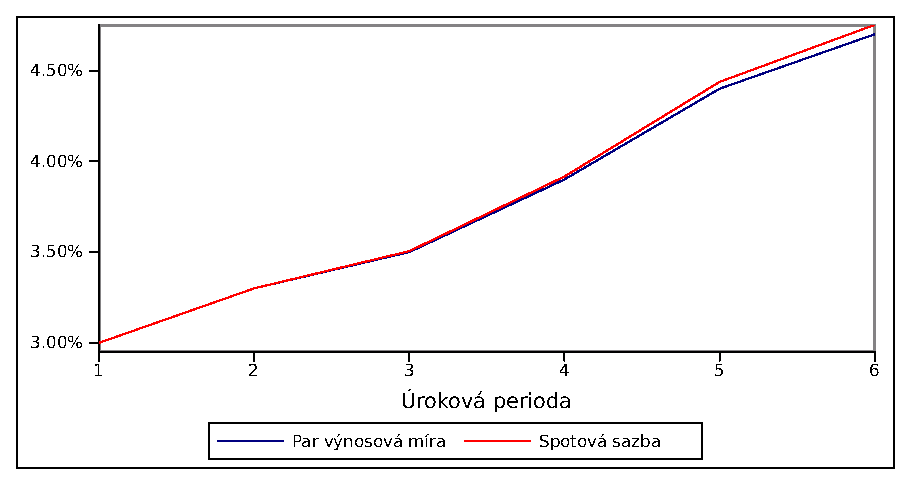
\includegraphics[scale=0.75]{spot_curve.eps}
  \caption{Spotová křivka zkonstruovaná metodou bootstraping}
  \label{spot_curve}
\end{figure}

Před výpočtem spotové křivky je třeba zvolit bázi, která je zpravidla koresponduje frekvencí výplaty kupónů podkladových dluhopisů. Jestliže bychom namísto půlroční báze zvolili roční bázi, museli bychom nejprve přepočíst půlroční par výnosovou sazbu
\begin{gather*}
1 + \frac{0.030}{2} = (1 + i)^{0.5} \\
i = 0.03023
\end{gather*}
a roční par výnosovou sazbu
\begin{gather*}
\Bigg(1 + \frac{0.033}{2}\Bigg)^2 = 1 + i \\
i = 0.03327
\end{gather*}
Rovnice (6.2) by pak přešla do tvaru
\begin{gather*}
\frac{1.75}{(1 + 0.03023)^{0.5}} + \frac{1.75}{(1 + 0.03327)^1} + \frac{101.75}{(1 + i)^{1.5}} = 100 \\
i = 0.03536
\end{gather*}
Analogicky lze dopočíst zbytek spotové křivky.

Ve výše uvedeném příkladě jsme předpokládali, že známe par výnosovou míru pro všechny potřebné splatnosti. Protože na trhu je zpravidla obchodován omezený počet emisí státních dluhopisů, není tento předpoklad v praxi splněn. Například vláda Spojených států, která emituje pokladniční poukázky se splatností tři a šest měsíců a dluhopisy se splatností dva, pět a deset roků. Zbývající par výnosové míry je tak třeba odvodit pomocí interpolace. Nejčastěji je aplikována lineární interpolace, nicméně lze použít také polynomickou nebo exponenciální interpolaci.

Kromě státních dluhopisů je možné pro konstrukci spotové křivky použít také korporátní dluhopisy, které jsou zpravidla definovány kreditním ratingem, zemí původu a sektorem emitenta. Takovéto spotové křivky slouží jako benchmark pro posuzování výnosu korporátních dluhopisů pomocí tzv. z-spreadu, který je popsán níže.

\subsection{Výnosové spready vztažené ke spotové křivce}

Tradiční přístup k výnosovému spreadu korporátního dluhopisu spočívá v poměřování jeho výnosu do splatnosti s výnosem do splatnosti porovnatelného státního dluhopisu. Vraťme se k výše uvedené tabulce. V souladu s touto tabulkou má tříletý státní dluhopis par výnosovou míru 4.70\%. Uvažujme korporátní dluhopis se stejnými charakteristikami\footnote{Jedná se tedy o korporátní dluhopis s kupónovou sazbou 4.70\%, pololetní výplatou kupónových plateb a zbytkovou splatností tři roky.} a cenou 98\%. Výnos do splatnosti tohoto dluhopisu je roven 5.43\%. Rozdíl mezi oběma výnosovými mírami, nazývaný nominální spread, je roven 73 bps. Nevýhodou nominálního spreadu je, že
\begin{itemize}
\item nezohledňuje strukturu spotové křivky
\item předpokládá neměnnost spotové křivky až do splatnosti dluhopisu, což může vést k zavádějícím výsledkům v případě dluhopisů s vnořenou opcí
\end{itemize}

\subsubsection{Z-spread}

Nominální spread je definován jako rozdíl mezi výnosovou mírou korporátního dluhopisu a výnosovou mírou porovnatelného státního dluhopisu. Naproti tomu z-spread je definován jako spread, o který je paralelně posunout spotovou křivku tak, abychom aplikací arbitrážního přístupu k ocenění získali cenu kotovanou na trhu.

Uvažujme spotovou křivku, kterou jsem odvodili v přechozí kapitole a výše zmiňovaný korporátní dluhopis. Z-spread pro tento dluhopis je definován rovnicí
\begin{equation*}
\frac{2.35}{\Big(1 + \frac{0.0300 + s}{2}\Big)^1} + \frac{2.35 + s}{\Big(1 + \frac{0.0330 + s}{2}\Big)^2} + \frac{2.35}{\Big(1 + \frac{0.0351 + s}{2}\Big)^3} + \frac{2.35}{\Big(1 + \frac{0.0392 + s}{2} \Big)^4} +
\end{equation*}
\begin{equation*}
+ \frac{2.35}{\Big(1 + \frac{0.0444 + s}{2} \Big)^5} + \frac{102.35}{\Big(1 + \frac{0.0475 + s}{2} \Big)^6} = 98
\end{equation*}   
Řešením této rovnice pro $s$ získáme 73.2 bps. V našem konkrétním případě je rozdíl mezi nominálním spreadem a z-spreadem zanedbatelný. Tento rozdíl je dán tvarem spotové křivky a charakteristikou dluhopisu. Pro spotovou křivku platí, že čím strmější křivka, tím větší je rozdíl mezi nominální spreadem a z-spreadem. Co se typu dluhopisu týče, v případě MBS popř. ABS, které jsou typické průběžným splácením nominální hodnoty, je rozdíl mezi nominálním spreadem a z-spreadem výraznější než v případě standardního kupónového dluhopisu.

Vedle spotové křivky zkonstruované ze státních dluhopisů je možné použít jako benchmark také spotové křivky zkonstruované z vybraných korporátních dluhopisů. Velmi často je z-spread vztahován také k tzv. swapové křivce\footnote{Základním stavebních kamenem swapové křivky jsou tzv. swapové sazby. Swapové sazby jsou, podobně jako ceny dluhopisů, kótovány trhem a představují cenu úrokového swapu. Úrokovými swapy a dalšími úrokovými deriváty se zabývají kapitoly 13 a 14.}.

\subsubsection{OAS spread}

Z-spread je založen na předpokladu konstatní spotové křivky. V případě dluhopisů s vnořenou úrokovou opcí je však tento předpoklad příliš svazující. Změna úrokových sazeb má totiž za následek nejen změnu současné hodnoty budoucího cash-flow ale také změnu cash-flow samotného. Jako příklad uvažujme svolatelný dluhopis, který může být emitentem svolán v případě poklesu úrokových sazeb. Toto omezení se snaží obejít OAS spread.

V případě konstantních úrokových sazeb by hodnota vnořené opce byla rovněž konstantní. Skutečný výnosový spread realizovaný investorem oproti spotové křivce by tak odpovídal z-spreadu. V reálném svetě, kde připouštíme pohyb úrokových sazeb, se hodnota vnořené opce a tím pádem také hodnota dluhopisu mění. Protože hodnota dluhopisu je klíčovým vstupem pro výpočet z-spreadu, zahrnuje tento spread také hodnotu vnořené opce. Připomeňme, že OAS spread je výnosový spread vztažený ke spotové křivce, který je upraven o případný vliv vnořené opce. Platí tedy
\begin{center}
\textit{z-spread = OAS spread + hodnota opce}
\end{center}
Pro danou míru kreditního rizika preferuje investor dluhopisy s vyšším spreadem. V případě dluhopisů s vnořenou opcí je však z-spread zkreslený o hodnotu vnořené opce. Proto by se měl investor v jejich případě spíše zaměřit na OAS spread.

Konkrétní postup výpočtu OAS spreadu se odvíjí od modelu pro ocenění dluhopisu s vnořenou opcí. Jako příklad uvažujme oceňovací model založený na binomickém úrokovém stromu. OAS spread má v tomto případě charakter paralelního posunu celého binomického stromu tak, aby se modelová cena dluhopisu rovnala jeho tržní ceně. K této problematice se vrátíme v kapitole 9.

\subsection{Forwardové úrokové sazby}

V předchozí kapitole jsem použili výnosovou křivku ke konstrukci spotové křivky. Ze spotové křivky pak lze vypočíst forwardové sazby, které mají charakter očekávaných budoucích úrokových sazeb.

\subsubsection{Výpočet forwardových úrokových sazeb}

Uvažujme investora s investičním horizontem jeden rok. První možností je nákup roční pokladniční poukázky a její držení do splatnosti. Alternativu představují dva po sobě jdoucí nákupy půlroční pokladniční poukázky. Protože jsou obě investice z pohledu podstupovaných rizik shodné, musí generovat shodný výnos. Podle pravidla jedné ceny a za předpokladu půlroční báze podkladové křivky tak musí platit
\begin{equation}
\Big(1 + \frac{i_{1Y}}{2} \Big)^2 = \Bigg(1 + \frac{i_{6M}}{2} \Bigg) \Bigg(1 + \frac{f_{6M,1Y}}{2} \Bigg) 
\end{equation}
kde $f_{6M, 1Y}$ je forwardovou úrokovou sazbou platnou za půl roku po dobu půl roku. V kontextu čísel příkladu z předchozí kapitoly by forwardová úroková sazba byla rovna
\begin{gather*}
\Bigg(1 + \frac{0.033}{2} \Bigg)^2 = \Big(1 + \frac{0.030}{2} \Big) \Big(1 + \frac{f_{6M,1Y}}{2} \Big)\\
f_{6M,1Y} = 0.360044
\end{gather*}
Analogicky lze odvodit forwardové úrokové sazby pro následující časové periody.
\begin{center}
\begin{tabular}{c c c c}
\textbf{Splatnost} & \textbf{Úroková} & \textbf{Spotová} & \textbf{6M forwardová}\\
\textbf{v letech} & \textbf{perioda} & \textbf{sazba} & \textbf{sazba}\\
\hline
0.50 & 1 & 3.00000\% &          \\
1.00 & 2 & 3.30000\% & 3.60044\% \\
1.50 & 3 & 3.50531\% & 3.91656\% \\
2.00 & 4 & 3.91637\% & 5.15453\% \\
2.50 & 5 & 4.43757\% & 6.53575\% \\		
3.00 & 6 & 4.75202\% & 6.33151\%
\end{tabular}
\end{center}
\begin{figure}
  \centering
  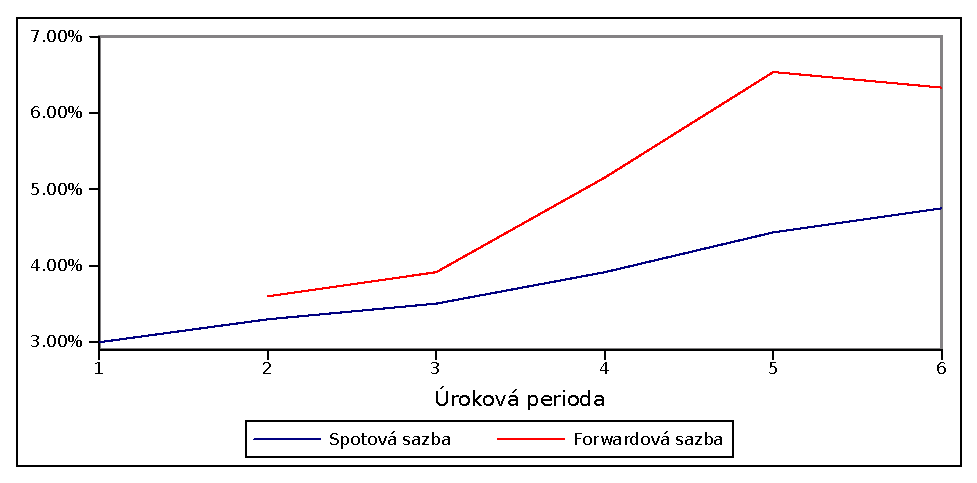
\includegraphics[scale=0.75]{forward_curve.eps}
  \caption{Křivka šestiměsíčních forwardových úrokových sazeb}
  \label{spot_curve}
\end{figure}
Pokud bychom namísto spotové křivky s půlroční bází uvažovali spotovou křivku s roční bází, přešla by rovnice (6.3) do tvaru
\begin{equation*}
1 + i_{1Y} = (1 + i_{6M})^{0.5} (1 + f_{6M,1Y})^{0.5} 
\end{equation*}
a forwardová úroková sazba $f_{6M,1Y}$ je rovna 3.632\%.
\begin{gather*}
1 + 0.03327 = (1 + 0.03023)^{0.5} (1 + f_{6M,1Y})^{0.5}\\
f_{6M,1Y} = 0.03632
\end{gather*}

\subsubsection{Oceňování pomocí forwardových úrokových sazeb}

Protože na spotové sazby lze pohlížet jako na soubor forwardových úrokových sazeb\footnote{Toto tvrzení je přímým důsledkem způsobu výpočtu forwardových úrokových sazeb.}, je lhostejné, zda-li budoucí cash-flow diskontujeme pomocí spotové sazby nebo odpovídajících forwardových úrokových sazeb.

Uvažujme spotovou křivku s půlroční bází z ní odvozené šestiměsíční forwarodové sazby. Vztah mezi spotovou sazbou a forwardovými úrokovými sazbami je dán rovnicí
\begin{equation*}
\Bigg(1 + \frac{i_{tY}}{2} \Bigg)^{2t} = \prod_{k = 0}^{2t-1} \Bigg(1 + \frac{f_{6M, \frac{1}{2}kY}}{2} \Bigg)
\end{equation*}
kde $i_{tY}$ je spotová sazba se splatností v čase $t$, $f_{6M,\frac{1}{2}kY}$ je šestiměsíční forwardová úroková sazba platná časovou peridu $\frac{1}{2}kY$ až $\frac{1}{2}(k + 1)Y$ a $f_{6M,0Y} = i_{{1}{2}Y}$. Současná hodnota částky 1~USD splatné v roce $t$ je
\begin{equation*}
\frac{1}{\Big(1 + \frac{i_{tY}}{2} \Big)^{2t}}
\end{equation*}
resp. s využitím výše uvedeného vztahu
\begin{equation}
\frac{1}{\prod_{k = 0}^{2t-1} \big(1 + \frac{f_{6M, \frac{1}{2}kY}}{2} \big)}
\end{equation}
Diskontní faktor (6.3) lze také vyjádřit ve tvaru
\begin{equation*}
\prod_{k = 0}^{2t-1} \frac{1}{\big(1 + \frac{f_{6M, \frac{1}{2}kY}}{2} \big)}
\end{equation*}
kde
\begin{equation*}
\frac{1}{\big(1 + \frac{f_{6M, \frac{1}{2}kY}}{2} \big)}
\end{equation*}
lze chápat jako forwardový diskontní faktor, který vyjadřuje hodnotu částky 1~USD v čase $\frac{1}{2}k$ za předpokladu, že investor tuto částku obdrží v čase $\frac{1}{2}(k+1)$.

\chapter{Úvod do měření úrokového rizika}

\section{Úvod}

V kapitole 2 jsme diskutovali úrokové riziko spojené s dluhopisy. Víme, že hodnota dluhopisu je negativně korelovaná s pohybem úrokových sazeb - růst úrokových sazeb implikuje pokles hodnoty dluhopisu a naopak. V této kapitole si ukážeme, jak toto úrokové riziko kvantifikovat.

\section{Metoda přecenění dluhopisu}

První metodou, která nás v souvislosti s kvantifikací úrokové rizika pravděpodobně napadne, je ocenění dluhopisu pro výchozí úroveň úrokových sazeb, posunutí úrokových sazeb a následné přecenění dluhopisu. Rozdíl mezi oběma oceněními pak představuje úrokové riziko v dolarovém vyjádření.

V případě, že máme správný oceňovací model, je tento přístup nejlepším možným. Jeho výhodou je velká flexibilita, která umožňuje implementovat nejrůznější scénáře vývoje úrokových sazeb a přesná kvatifikace dopadu změny úrokových sazeb do ocenění dluhopisu. Tento přístup lze nejen na plain-vanilla dluhopisy ale také na dluhopisy s vnořenou opcí. Nevýhodou metody přecenění dluhopisu je jeho relativně značná výpočetní náročnost. Tento nedostatek odstraňuje alternativní metoda kvatifikace úrokového rizika - tzv. durace a konvexita dluhopisu.

\section{Durace a konvexita dluhopisu}

Durace je aproximace změny hodnoty dluhopisu v závislosti na změně jeho výnosové míry do splatnosti. Tuto aproximaci lze dále zpřesnit pomocí zohledněním tzv. konvexity dluhopisu.

\subsection{Vztah mezi hodnotou dluhopisu a výnosovou mírou do splatnosti}

V následujícím textu se budeme zabývat vztahem mezi hodnotou dluhopisu a výnosovou mírou do splatnosti. Tento vztah budeme demonstrovat na příkladě plain-vanilla fixního dluhopisu, svolatelného dluhopisu a dluhopisu s právem zpětného prodeje.

\subsubsection{Plain-vanilla fixní dluhopis}
Jestliže bychom vypočetli hodnotu plain-vanilla fixního dluhopisu pro různé výnosové míry do splatnosti a výsledky vynesli do grafu, získali bychom graf (\ref{bond_yield}). Z tohoto grafu je patrné, že pro plain-vanilla fixní dluhopis platí následující pravidla
\begin{itemize}
\item hodnota dluhopisu je klesající funkcí výnosové míry do splatnosti
\item tato funkce je konvexní funkcí pro všechny výnosové míry do splatnosti
\item v důsledku konvexity funkce je růst hodnoty dluhopisu v případě poklesu výnosové míry do splatnosti výraznější než pokles hodnoty dluhopisu v případě růstu výnosové míry do splatnosti 
\end{itemize}
\begin{center}
\begin{figure}
\begin{pspicture}(0,0)(7.0,9.0)
\psline[arrows=->](1.0,1.0)(8.5,1.0)
\psline[arrows=->](1.0,1.0)(1.0,6.5)

\pscurve(1.0,6.0)(3.5,3.5)(8.5,2.0)

\psline[linestyle=dotted](3.5,3.5)(3.5,0.9)

\rput(8.0,0.7){výnos do splatnosti}
\rput(2.0,6.8){hodnota dluhopisu}

\rput(8.5,2.2){\tiny{$a$}}
\rput(1.2,6.2){\tiny{$a'$}}

\rput(3.5,0.7){\tiny{$i$}}

\rput(6.5,5.0){\tiny{$a'a$ - plain-vanilla fixní dluhopis}}

\end{pspicture}
\caption{Vztah mezi výnosovou mírou do splatnosti a hodnotou plain-vanilla fixního dluhopisu}
\label{bond_yield}
\end{figure}
\end{center}
Třetí tvrzení lze také formulovat následovně. Uvažujme plain-vanilla fixní dluhopis s výchozí úrovní výnosové míry do splatnosti $i$ a jí odpovídající hodnotě $P$. Dále uvažujme výnosové míry $i_l$ a $i_h$ a jim odpovídající hodnoty dluhopisu $P_l$ a $P_h$ takové, že $i_l < i < i_h$ a $i - i_l = i_h - i$. Pro hodnoty dluhopisů pak platí $P_l < P < P_h$ a $P - P_l < P_h - P$. Tvrzení ilustruje obrázek (\ref{bond_yield_relationship_convex}).
\begin{center}
\begin{figure}
\begin{pspicture}(0,0)(7.0,9.0)
\psline[arrows=->](1.0,1.0)(8.5,1.0)
\psline[arrows=->](1.0,1.0)(1.0,6.5)
\pscurve(1.0,6.0)(3.5,3.5)(8.5,2.0)

\psline[linestyle=dashed](0.9,3.5)(3.5,3.5)
\psline[linestyle=dashed](3.5,0.9)(3.5,3.5)

\psline[linestyle=dotted](5.5,0.9)(5.5,2.7)
\psline[linestyle=dotted](0.9,2.7)(5.5,2.7)

\psline[linestyle=dotted](1.5,0.9)(1.5,5.4)
\psline[linestyle=dotted](0.9,5.4)(1.5,5.4)

\rput(1.5,0.7){\tiny{$i_l$}}
\rput(3.5,0.7){\tiny{$i$}}
\rput(5.5,0.7){\tiny{$i_h$}}

\rput(0.7,2.7){\tiny{$P_l$}}
\rput(0.7,3.5){\tiny{$P$}}
\rput(0.7,5.4){\tiny{$P_h$}}

\rput(6.0,4.0){\tiny{$i - i_l = i_h - i$}}
\rput(6.0,3.5){\tiny{$P - P_l < P_h - P$}}

\rput(8.0,0.7){výnos do splatnosti}
\rput(2.0,6.8){hodnota dluhopisu}

\end{pspicture}
\caption{Konvexní funkce hodnoty dluhopisu - vztah mezi hodnotou a výnosovou mírou do splatnosti}
\label{bond_yield_relationship_convex}
\end{figure}
\end{center}

\subsubsection{Dluhopis s vnořenou opcí}

V případě dluhopisu s vnořenou opcí neodpovídá tvar funkce hodnoty dluhopisu obrázku (\ref{bond_yield}).

Uvažujme svolatelný dluhopis, který lze rozložit na podkladový plain-vanilla fixní dluhopis a úrokovou opci. Při poklesu tržních výnosových měr na jedné straně vzroste cena podkladového dluhopisu, na druhé straně také vzroste hodnota vnořené úrokové opce, která umožňuje investorovi dluhopis předčasně svolat a refinancovat se za výhodnějších podmínek. Předpokládejme, že hodnota této opce je až do výnosové míry $i$  nulová. Pro výnosovou míru do splatnosti vyšší nebo rovnu $i$ se tak hodnota svolatelného dluhopisu shoduje s hodnotou plain-vanilla dluhopisu. Pro výnosovou míru do splatnosti vyšší než $i$ je hodnota vnořené opce kladná, a proto je hodnota svolatelného dluhopisu nižší než je hodnota podkladového plain-vanilla fixního dluhopisu. Hodnotu svolatelného dluhopisu v závislosti na výnosové míře do splatnosti ilustruje obrázek (\ref{callable_bond_yield}).
\begin{center}
\begin{figure}
\begin{pspicture}(0,0)(7.0,9.0)
\psline[arrows=->](1.0,1.0)(8.5,1.0)
\psline[arrows=->](1.0,1.0)(1.0,6.5)

\pscurve(1.0,6.0)(3.5,3.5)(8.5,2.0)
\pscurve[linestyle=dashed](1.0,4.7)(2.2,4.3)(3.5,3.5)

\psline[linestyle=dotted](3.5,3.5)(3.5,0.9)

\rput(8.0,0.7){výnos do splatnosti}
\rput(2.0,6.8){hodnota dluhopisu}

\rput(8.5,2.2){\tiny{$a$}}
\rput(1.2,6.2){\tiny{$a'$}}

\rput(3.5,3.8){\tiny{$b'$}}
\rput(1.2,4.9){\tiny{$b$}}

\rput(3.5,0.7){\tiny{$i$}}

\rput(6.5,5.0){\tiny{$a'a$ - podkladový plain-vanilla fixní dluhopis}}
\rput(6.5,5.3){\tiny{$ba$ - svolatelný dluhopis}}

\end{pspicture}
\caption{Vztah mezi výnosovou mírou do splatnosti a hodnotou svolatelného dluhopisu}
\label{callable_bond_yield}
\end{figure}
\end{center}
Pro konkávní část funkce hodnoty svolatelného dluhopisu\footnote{Konkávní část funkce hodnoty svolatelného dluhopisu je v ilustračním obrázku (\ref{callable_bond_yield}) označena jako $bb'$.} je růst hodnoty dluhopisu z titulu poklesu výnosové míry menší než pokles hodnoty dluhopisu z titulu růstu výnosové míry. V souvislosti s touto vlastností svolatelných dluhopisů hovoříme jako o negativní konvexitě. Tvrzení ilustruje obrázek (\ref{bond_yield_relationship_concave}). Připomeňme, že hodnota plain-vanilla fixního dluhopisu je konvexní, a proto pro ni platí opačné tvrzení.
\begin{center}
\begin{figure}
\begin{pspicture}(0,0)(7.0,9.0)

\psline[arrows=->](1.0,1.0)(8.5,1.0)
\psline[arrows=->](1.0,1.0)(1.0,6.5)
\pscurve(1.0,6.0)(4.5,5.5)(8.5,2.0)

\psline[linestyle=dashed](0.9,5.5)(4.5,5.5)
\psline[linestyle=dashed](4.5,0.9)(4.5,5.5)

\psline[linestyle=dotted](0.9,4.9)(5.5,4.9)
\psline[linestyle=dotted](5.5,0.9)(5.5,4.9)

\psline[linestyle=dotted](0.9,5.8)(3.5,5.8)
\psline[linestyle=dotted](3.5,0.9)(3.5,5.8)

\rput(3.5,0.7){\tiny{$i_l$}}
\rput(4.5,0.7){\tiny{$i$}}
\rput(5.5,0.7){\tiny{$i_h$}}

\rput(0.7,4.9){\tiny{$P_l$}}
\rput(0.7,5.5){\tiny{$P$}}
\rput(0.7,5.8){\tiny{$P_h$}}

\rput(7.5,5.0){\tiny{$i - i_l = i_h - i$}}
\rput(7.5,4.7){\tiny{$P - P_l > P_h - P$}}

\rput(8.0,0.7){výnos do splatnosti}
\rput(2.0,6.8){hodnota dluhopisu}

\end{pspicture}
\caption{Vztah mezi výnosovou mírou do splatnosti a hodnotou svolatelného dluhopisu pro konkávní část funkce}
\label{bond_yield_relationship_concave}
\end{figure}
\end{center}

Uvažujme dluhopis se zpětným právem prodeje který lze rozložit na podkladový plain-vanilla fixní dluhopis a vnořenou úrokovou opci, která umožňuje majiteli zpětně prodat dluhopis emitentovi za předem dohodnutou cenu. Je zřejmé, že hodnota této opce roste s rostoucí tržní výnosovou mírou, protože umožňuje majiteli dluhopisu reinvestovat finanční prostředky za výhodnějších podmínek na trhu. Předpokládejme, že pro výnosovou míru menší nebo rovnu $i$, je hodnota vnořené opce nulová. Na tomto intervalu je tedy hodnota dluhopisu s právem zpětného prodeje stejná jako hodnota podkladového plain-vanilla fixního dluhopisu. Pro výnosovou míru do splatnosti vyšší než $i$, je hodnota vnořené opce kladná, a proto je hodnota dluhopisu s právem zpětného prodeje vyšší než hodnota podkladového plain-vanilla fixního dluhopisu. Situaci ilustruje obrázek (\ref{putable_bond_yield}).
\begin{center}
\begin{figure}
\begin{pspicture}(0,0)(7.0,9.0)
\psline[arrows=->](1.0,1.0)(8.5,1.0)
\psline[arrows=->](1.0,1.0)(1.0,6.5)





















\pscurve(1.0,6.0)(3.5,3.5)(8.5,2.0)
\pscurve[linestyle=dashed](3.5,3.5)(5.0,3.2)(8.5,3.0)

\psline[linestyle=dotted](3.5,3.5)(3.5,0.9)

\rput(8.0,0.7){výnos do splatnosti}
\rput(2.0,6.8){hodnota dluhopisu}

\rput(8.5,2.2){\tiny{$a$}}
\rput(1.2,6.2){\tiny{$a'$}}

\rput(3.5,3.8){\tiny{$b'$}}
\rput(8.5,3.2){\tiny{$b$}}

\rput(3.5,0.7){\tiny{$i$}}

\rput(6.5,5.0){\tiny{$a'a$ - podkladový plain-vanilla fixní dluhopis}}
\rput(6.5,5.3){\tiny{$a'b$ - dluhopis s právem zpětného prodeje}}

\end{pspicture}
\caption{Vztah mezi výnosovou mírou do splatnosti a hodnotou dluhopisu}
\label{putable_bond_yield}
\end{figure}
\end{center}

\subsection{Matematické odvození durace a konvexity}

Uvažujme fixně úročený dluhopis s roční výplatou kupónů. Jeho hodnotu lze chápat jako funkci
\begin{equation*}
f(i) = \sum_{t = 1}^T \frac{CF_t}{(1 + i)^t}
\end{equation*}
kde $i$ představuje výnosovou míru do splatnosti, $T$ splatnost dluhopisu v letech a $CF_t$ je cash-flow generované dluhopisem na konci roku $t$. Protože je $f(i)$ hladnou funkcí podle $i$, lze s pomocí Taylorova rozvoje výjádřit změnu hodnoty dluhopisu pro výnosovou míru do splatnosti $i + \Delta i$ jako
\begin{equation*}
f(i) - f(i + \Delta i) = \sum_{k=1}^{\infty}\frac{1}{k!} \frac{\partial^k f(i)}{\partial i^k} \big( \Delta i \big)^k
\end{equation*}
V případě, že se omezíme pouze na prvních $l$ členů rozvoje, platí přibližně
\begin{equation*}
f(i) - f(i + \Delta i) \approx \sum_{k=1}^{l}\frac{1}{k!} \frac{\partial^k f(i)}{\partial i^k} \big( \Delta i \big)^k
\end{equation*}
V praxi se pro odhad změny hodnoty dluhopisu používá nejčastěji první a druhý člen aproximace. Člen
\begin{equation}
\frac{\partial f(i)}{\partial i} = \sum_{t = 1}^T -t \frac{CF_t}{(1+i)^{t+1}}
\end{equation}
nazýváme durací a člen
\begin{equation}
\frac{\partial^2 f(i)}{\partial i^2} = \sum_{t = 1}^T t (t+1) \frac{CF_t}{(1+i)^{t+2}}
\end{equation}
nazýváme konvexitou. Pomocí durace lze změnu hodnoty dluhopisu v okolí výnosové míry do splatnosti $i$ aproximovat jako
\begin{equation*}
f(i) - f(i + \Delta i) \approx \sum_{t = 1}^T -t \frac{CF_t}{(1+i)^{t+1}} \Delta i
\end{equation*}
popř. zpřesnit pomocí konvexity
\begin{equation*}
f(i) - f(i + \Delta i) \approx \sum_{t = 1}^T \Bigg(- t \frac{CF_t}{(1+i)^{t+1}} \Delta i + \frac{1}{2} t (t+1) \frac{CF_t}{(1+i)^{t+2}} \big( \Delta i \big)^2 \Bigg)
\end{equation*}
Aproximaci hodnoty dluhopisu pomocí durace a konvexity v okolí výnosové míry do splatnosti $i$ ilustruje obrázek (\ref{duration_convexity}).

\begin{center}
\begin{figure}
  \centering
  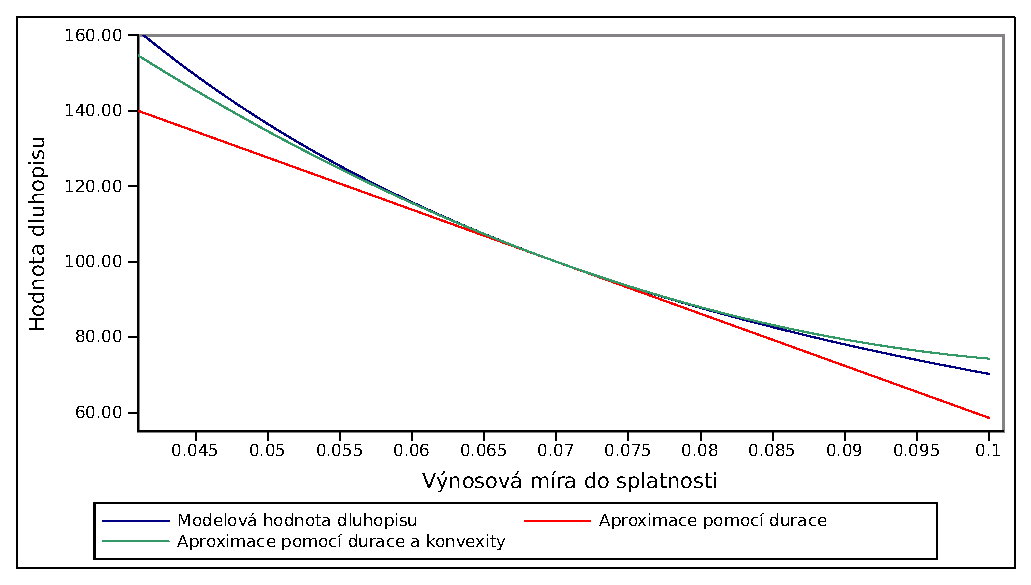
\includegraphics[scale=0.75]{duration_convexity.eps}
  \caption{Aproximace hodnoty dluhopisu pomocí durace a konvexity}
  \label{duration_convexity}
\end{figure}
\end{center}

\subsection{Numerický výpočet durace a konvexity}

Rovnice (7.1) a (7.2) pro výpočet durace a konvexity lze použít pouze pro plain-vanilla fixní dluhopisy. V případě dluhopisů s vnořenou opcí nemusí existovat uzavřené varianty těchto rovnic. Nicméně pro dluhopisy s vnořenou opcí lze vypočíst duraci a konvexitu numericky.

\subsubsection{Durace}

Durace vyjadřuje citlivost hodnoty dluhopisu na změnu výnosové míry do splatnosti. Duraci lze numericky vyjádřit jako
\begin{equation}
D = \frac{V^{+} - V^{-}}{2 \Delta i}
\end{equation}
kde $V^{+}$ je hodnota dluhopisu pro úroveň výnosové míry do splatnosti $i + \Delta i$ a $V^{-}$ je hodnota dluhopisu pro úroveň výnosové míry do splatnosti $i - \Delta i$. Takto definovaná durace představuje dolarovou změnu hodnoty dluhopisu při poklesu výnosové míry o jeden procentní bod.

Uvažujme pětiletý dluhopis s roční výplatou kupónu, kupónovou sazbou 5\% a nominální hodnotou 100~USD. Předpokládejme, že výchozí úroveň výnosové míry do splatnosti je 5\% - hodnota dluhopisu je tak rovna jeho nominální hodnotě. Pro změnu výnosové míry o 5 bazických bodů je hodnota dluhopisu $H^{-}$ rovna 100.217~USD a hodnota dluhopisu $H^{+}$ rovna 99.784~USD. Durace vypočtená dle (7.3) je tak rovna -433.
\begin{equation*}
\frac{99.784 - 100.217}{2 \times 0.0005} = -433
\end{equation*}
Pro modelový dluhopis a nárůst výnosové míry o 5 bazických bodů lze s pomocí durace odhadnout pokles hodnoty dluhopisu na 0.2165~USD.
\begin{equation*}
-433 \times 0.0005 = -0.2165
\end{equation*}
Hodnota dluhopisu tak klesne z výchozí úrovně 100.000~USD na 99.784~USD, což odpovídá skutečné změně hodnoty dluhopisu.

\subsubsection{Konvexita}

Pokud bychom chtěli kvantifikovat změnu hodnotu dluhopisu pro změnu výnosové míry v řádu stovek bazických bodů, je odhad pomocí durace méně přesný. Uvažujme situaci, kdy výnosová míra do splatnosti vzroste o 250 bazických bodů. Jestliže bychom pro odhad poklesu hodnoty dluhopisu použili pouze duraci, získali bychom výsledek 10.825~USD
\begin{equation*}
-433 \times 0.025 = -10.825
\end{equation*}
však ve skutečnosti se cena dluhopisu sníží o 10.004~USD. Odhad lze zpřesnit pomocí konvexity, kterou lze vypočíst na základě rovnice
\begin{equation}
C = \frac{V^{-} + V^{+} - 2 V}{\big( \Delta i\big)^2}
\end{equation}
Pro plain-vanilla fixní dluhopis platí, že nárůst hodnoty v důsledku poklesu výnosové míry je vyšší než pokles jeho hodnoty v důsledku růstu výnosové míry. Z tohoto důvodu je konvexita definovaná skrze (7.4) kladná. V případě svolatelného dluhopisu, pro který tento předpoklad splněn není, je konvexita záporná. Tuto vlastnost svolatelného dluhopisu jsme diskutovali ve výše uvedeném textu.

V našem konkrétním případě je konvexita modelového dluhopisu rovna 4000.
\begin{equation*}
\frac{99.784 + 100.217 - 2 \times 100}{2 \times 0.0005^2} = 4000
\end{equation*}
Jestliže pro odhad změny hodnoty dluhopisu vedle durace použijeme také konvexitu, získáme odhad poklesu ve výši 10.200~USD.
\begin{equation*}
-433 \times 0.025 + 0.5 \times 2000 \times 0.025^2 = -10.200
\end{equation*}

\subsubsection{Porovnání analytického a numerického výpočtu durace a konvexity}

V předchozím textu jsme s pomocí numericky vypočtené durace a konvexity odhadli změnu hodnoty modelového dluhopisu při růstu jeho výnosové míry do splatnosti o 250 bps na -10.200~USD.

Změnu hodnoty modelového dluhopisu lze odhadnout také pomocí analyticky odvozené durace a konvexity. Připomeňme, že hodnota modelového dluhopisu je dána rovnicí
\begin{equation*}
f(i) = \sum_{t = 1}^T \frac{CF_t}{(1+i)^t}
\end{equation*}
Aplikací (7.1) na funkci hodnoty dluhopisu získáme duraci
\begin{equation*}
\frac{-1 \times 5}{(1+0.05)^2} +  \frac{-2 \times 5}{(1+0.05)^3} +  \frac{-3 \times 5}{(1+0.05)^4} +  \frac{-4 \times 5}{(1+0.05)^5} +  \frac{-5 \times 5}{(1+0.05)^6} = -432.948
\end{equation*}
a aplikací (7.2) pak konvexitu
\begin{equation*}
\frac{1 \times 2 \times 5}{(1+0.05)^3} + \frac{2 \times 3 \times 5}{(1+0.05)^4} + \frac{3 \times 4 \times 5}{(1+0.05)^5} + \frac{4 \times 5 \times 5}{(1+0.05)^6} + \frac{5 \times 6 \times 105}{(1+0.05)^7} = 2393.599
\end{equation*}
Pokles hodnoty modelového dluhopisu bychom s pomocí výše vypočtené durace a konvexity odhadli na 10.076~USD.
\begin{equation*}
-432.948 \times 0.025 + 0.5 \times 2393.599 \times 0.025^2 = -10.076
\end{equation*}
Ve skutečnosti poklesla hodnota dluhopisu o 10.004~USD.

\subsection{Typy durace}

\subsubsection{Dolarová durace}

Až dosud jsem duraci interpretovali jako změnu hodnoty dluhopisu v závislosti na změně výnosové míry do splatnosti. Duraci, které měří změnu hodnoty dluhopisu v peněžních jednotkách, nazýváme dolarovou durací.

\subsubsection{Modifikovaná durace}

Modifikovaná durace je definovaná jako relativní změna hodnoty dluhopisu v případě, že výnosová míra do splatnosti vzroste o jeden procentní bod. Modifikovaná durace je tak definována jako
\begin{equation*}
D_M = \frac{D_{\$}}{V_0}
\end{equation*}

kde $D_{\$}$ je dolarová durace a $V_0$ je výchozí hodnota dluhopisu. Jestliže chceme výsledek zpřesnit pomocí konvexity, je nutné použít modifikovanou konvexitu
\begin{equation*}
C_M = \frac{C_{\$}}{V_0}
\end{equation*}
kde $C_{\$}$ je dolarová konvexita definovaná v předchozí kapitole.

\subsubsection{Efektivní durace}

Dolarová a modifikovaná durace předpokládají, že změna úrokových sazeb nemá za následek změnu cash-flow generovaného dluhopisem. Tento předpoklad není splněn pro dluhopisy s vnořenou úrokovou opcí - aplikace dolarové popř. modifikované durace by mohlo vést k zavádějícím výsledkům. Pro odhad změny hodnoty těchto dluhopisů je možné použít rovnici (7.3), kde $V^{+}$ a $V^{-}$ jsou vypočteny pomocí vhodného oceňovací modelu zohledňujícího dopad změny úrokových sazeb na cash-flow dluhopisu. Takto definovanou duraci nazýváme efektivní durací. Analogicky k efektivní duraci je možné vypočíst na základě (7.4) také efektivní konvexitu.

\subsubsection{Macaulayova durace}

V roce 1938 zformuloval Macaulay míru citlivosti ceny plain-vanilla fixního dluhopisu na změnu výnosové míry do splatnosti jako
\begin{equation}
D_{mac} = -\frac{1}{kV_0}\sum_{t=1}^{kT} t\frac{CF_t}{(1 + \frac{i}{k})^t}
\end{equation}
kde $i$ výnosová míra do splatnosti, $k$ frekvence výplaty kupónových plateb a $CF_t$ cash-flow generované dluhopisem. 
Vzhledem k tomu, že obecná funkce hodnoty plain-vanilla dluhopisu je dána rovnicí
\begin{equation*}
f(i) = \sum_{t = 1}^{kT} \frac{CF_t}{(1+\frac{i}{k})^t}
\end{equation*}
je modifikovaná durace pro tento dluhopis odvozená z (7.1) rovna
\begin{equation*}
D_M = -\frac{1}{k V_0}\sum_{t = 1}^{kT} t \frac{CF_t}{(1 + \frac{i}{k})^{t+1}}
\end{equation*}
Mezi Macaulayovou durací definovanou (7.5) a modifikovanou durací tedy platí následující rovnice
\begin{equation*}
D_{mac} = D_M \Big( 1 + \frac{i}{k} \Big) 
\end{equation*}
Z tohoto vztahu vyplývá, že Macaulayova durace, stejně jako dolarová a modifikovaná durace, nezohledňuje případnou změnu cash-flow dluhopisu z titulu změny úrokových sazeb.

Z rovnice (7.1) je zřejmé, že modifikovaná durace diskotního dluhopisu je rovna
\begin{equation*}
D_{mac} = D_M (1 + i) = -\frac{T \times \frac{N_T}{(1 + i)^{T+1}}}{\frac{N_T}{(1 + i)^T}}(1+i) = -T
\end{equation*}
\begin{equation*}
D_M \approx -T
\end{equation*}

\subsection{Interpretace durace}

\subsubsection{Durace jako změna hodnoty dluhopisu}

Duraci jsme definovali jako dolarovou popř. relativní změnu hodnoty dluhopisu při změně jeho výnosové míry do splatnosti o jeden procentní bod. Toto je nejběžnější a nejsrozumitelnější definice durace. Kromě této definice existují také definice alternativní.

\subsubsection{Durace jako první derivace funkce hodnoty dluhopisu}

Duraci lze také chápat jako první derivaci funkce hodnoty dluhopisu. V případě plain-vanilla fixního dluhopisu se jedná o definici skrze rovnici (7.1). Tato definice, ač z matematického hlediska naprosto správná, má několik nevýhod. První nevýhodou je, že v případě složitějších dluhopisů nemusí existovat první derivace funkce jejich hodnoty v uzavřené formě. To znamená, že duraci není možné vyjádřit ve formě jednoho vzorečku. Další nevýhodou je nižší míra srozumitelnosti pro klienty. Definice durace jako míra citlivosti hodnoty dluhopisu na změnu úrokových sazeb je pochopitelná i pro neodborníky. Na druhou stranu pochopení definice durace jako první derivace funkce hodnoty dluhopisu vyžaduje určité, byť základní, znalosti kalkulu. Z tohoto důvodu je obecně preferovaná první varianta definice durace dluhopisu. 

\subsubsection{Durace jako střední doba do splatnosti dluhopisu}

Tato definice durace vychází z rovnice (7.5), kde je cash-flow dluhopisu ''váženo" časem. Tato definice je však ze všech možný nejméně šťastnou. Tato definice je z praktického hlediska bezcenná, protože nám neříká nic o rizikovosti dluhopisu. Pokud bychom trvali na definici durace jako měřítka času, je vhodnější definovat duraci pomocí fiktivního diskontního dluhopisu. Jestliže durace zkoumaného dluhopisu vyjde rovna například 5.92, má tento dluhopisu stejnou citlivost na změnu úrokových sazeb jako diskontní dluhopis se zbytkovou splatností 5.92 let. Tím však narážíme na další slabou stránku této definice - existují totiž dluhopisy, jejichž durace je záporná\footnote{Platby generované MBS je možné rozdělit na úrokové platby a splátky jistiny. V návaznosti na to je možné z MBS vytvořit interest-only MBS, do kterého jsou směřovány úrokové platby a principal-only MBS, do kterého jsou směřovány splátky jistiny. Interest-only MBS je pak příkladem dluhopisu se zápornou durací.}. Diskontní dluhopis se zápornou dobou splatnosti pochopitelně neexistuje.

\subsection{Durace dluhopisového portfolia}

Protože je cash-flow generované portfoliem aditivní, je aditivní také durace dluhopisů, které toto portfolio tvoří. Dolarovou duraci portfolia tak lze vyjádřit jako
\begin{equation*}
D_{\$}^P = \sum_{i = 1}^n p_i D_{\$}^i
\end{equation*}
kde $n$ představuje počet dluhopisů v portfoliu, $p_i$ počet kusů $i$-tého dluhopisu v rámci portfolia a $D_{\$}^i$ je dolarová durace $i$-tého dluhopisu. Modifikovanou duraci lze analogicky definovat jako
\begin{equation*}
D_M^P = \sum_{i = 1}^n w_i D_M^i
\end{equation*}
kde $w_i$ je podíl tržní hodnoty $i$-tého dluhopisu na celkové tržní hodnotě portfolia.

Za definicí durace portfolia je schován předpoklad, že se výnosová míra do splatnosti všech podkladových dluhopisů změní o stejný počet bazických bodů. To jinými slovy znamená, že výnosové míry do splatnosti jednotlivých dluhopisů musí být dokonale korelovány. V opačném případě takto definovaná míra citlivosti portfolia na změnu úrokových sazeb postrádá smysl.

\subsection{Citlivost na jeden bazický bod}

Dolarová durace představuje změnu hodnoty dluhopisu vyjádřenou v peněžních jednotkách při změně vnitřní výnosové míry o jeden procentní bod neboli o 100 bps. V praxi je možné se setkat s podobným ukazatelem. Jedná se o tzv. ''price value of a basis point" nazývanou též ''dolar value of 01" (DV01), která vyjadřuje změnu hodnoty finančního aktiva v peněžních jednotkách při změně jeho výnosové míry o jeden bazický bod. Jedná se tedy o specifický případ dolarové durace, kdy do rovnice (7.3) dosadíme $\Delta i = 0.0001$.

\subsection{Význam volatility výnosové míry}

Dolarová durace plain-vanilla fixního dluhopisu je definovaná jako
\begin{equation*}
D_{\$} = -\frac{1}{k} \sum_{t=1}^{kT} t\frac{c}{(1 + \frac{i}{k})^{t+1}} - T\frac{1}{(1 + \frac{i}{k})^{kT + 1}}
\end{equation*}
Z výše uvedeného vzorce je patrné, že dolarová durace je tak tím vyšší, čím vyšší je výnosová míra do splatnosti. Tento závěr je patrný také z obrázku (\ref{bond_yield}), kdy je změna hodnoty dluhopisu, za předpokladu konstantní změny výnosové míry do splatnosti, vyšší pro nižší úrovně výnosové míry a naopak nižší pro vyšší úrovně výnosové míry. To je dáno skutečností, že hodnota dluhopisu jako funkce výnosové míry do splatnosti má konvexní tvar.

Uvažujme státní a korporátní dluhopis. Předpokládejme, že oba dluhopisy mají půlroční frekvenci výplaty kupónů, zbytkovou splatnost deset let, nominální hodnotu 100~USD a jsou aktuálně obchodovány za par. Vzhledem k rozdílnému kreditnímu riziku musí být kupónová sazba a výnosová míra do splatnosti korporátního dluhopisu vyšší než výnosová míra do splatnosti státního dluhopisu. V souladu s výše uvedeným tvrzením by dolarová durace korporátního dluhopisu měla být nižší než modifikovaná durace státního dluhopisu. Pro ilustraci problematiky předpokládejme, že kupónová sazba a výnos do splatnosti jsou v případě státního dluhopisu rovny 3.00\% a v případě korporátního dluhopisu rovny 5.00\%. Dolarová durace státního dluhopisu je rovna -8.58~USD a korporátního dluhopisu -7.79~USD. Znamená tento závěr, že míra úrokového rizika korporátního dluhopisu je v porovnání se státním dluhopisem nižší?

Vysvětlení tohoto zdánlivého paradoxu souvisí se skutečností, že koncept modifikované durace předpokládá posun výnosové míry o stejný počet bazických bodů bez ohledu na její výchozí úroveň. V praxi však je však fluktuace výnosové míry vyjádřená v bazických bodech tím vyšší, čím vyšší je tato míra. Pravděpodobnost, že se výnosová míra posune z výchozí úrovně 5.00\% na úroveň 5.50\% je tak vyšší, než pravděpodobnost, že se výnosová míra posune z výchozí úrovně 3.00\% na úroveň 3.50\%. Tuto skutečnost je třeba vzít v potaz při porovnávání senzitivit s rozdílnou výnosovou mírou do splatnosti. Jedním z aplikovatelných přístupů je value-at-risk (VaR), který zahrnuje nejen citlivost dluhopisu na změnu výnosové míry, ale také volatilitu samotných výnosových měr.

\chapter{Časová struktura a volatilita úrokových sazeb}

\section{Úvod}

Klíčovou roli v oceňování dluhopisů hrají státní dluhopisy, které slouží jako reference při stanovení cen dluhopisů. Zároveň také určují minimální výnosovou míru, kterou jsou investoři ochotni akceptovat při nákupu dluhopisů. Spotová křivka zkonstruovaná z cen státních dluhopisů tak představuje základní vstup do oceňovacích modelů dluhopisů. V Evropě tuto roli často přejímá tzv. swapová křivka.

Časovou strukturou úrokových sazeb nejčastěji vztahuje k spotové křivce zkonstruované ze státních dluhopisů. Časovou strukturou spotové křivky rozumíme vztah mezi výnosovou mírou fiktivního diskontního dluhopisu a jeho dobou do splatnosti dle této křivky. V kapitole 2 jsme si představili základní teorie vysvětlující časovou strukturu úrokových sazeb. V této kapitole navážeme na tyto teorie s konceptem forwardových úrokových sazeb.

Na konci předešlé kapitoly jsme vysvětlili, proč je při kvantifikaci úrokového rizika kromě durace dluhopisu důležité zohlednit také volatilitu výnosových měr. V této kapitole si ukážeme jak kvantifikovat volatilitu výnosové míry a představíme si koncept tzv. úrokové durace, která představuje míru citlivosti dluhopisu na konkrétní segment spotové křivky.

\section{Profil a posun spotové křivky}

V následujícím textu si představíme profily a změny profilů spotové křivky, které byly pozorovány v minulosti.

\subsection{Profil spotové křivky}

Časovou strukturou nebo také profilem spotové křivky rozumíme vztah mezi výnosovou mírou do splatnosti a splatností fiktivního diskontního dluhopisu. V minulosti byly pozorovány čtyři základní profily spotové křivky
\begin{itemize}
\item rostoucí profil - výnosová míra roste se splatností
\item klesající profil - výnosová míra klesá se splatností
\item plochý profil - výnosová míra je přibližně stejná pro všechny splatnosti
\item zlomový profil - výnosová míra nejprve roste a následně klesá popř. nejprve klesá a následně roste
\end{itemize}
V praxi je nejobvyklejší rostoucí profil, nicméně poměrně často je možné se setkat se zlomovým profilem.
\begin{center}
\begin{figure}
\begin{pspicture}(0,0)(10.0,10.0)

\psline(0.5,5.0)(4.5,5.0)
\psline(0.5,5.0)(0.5,9.5)
\pscurve(0.7,5.3)(2.5,7.0)(4.5,8.0)
\rput(2.5,4.7){\tiny{(a)}}
\rput(0.9,9.6){\tiny{výnos}}
\rput(4.5,4.7){\tiny{splatnost}}

\psline(5.5,5.0)(9.5,5.0)
\psline(5.5,5.0)(5.5,9.5)
\pscurve(5.7,8.0)(7.5,6.0)(9.5,5.3)
\rput(7.5,4.7){\tiny{(b)}}
\rput(5.9,9.6){\tiny{výnos}}
\rput(9.5,4.7){\tiny{splatnost}}

\psline(0.5,0.5)(4.5,0.5)
\psline(0.5,0.5)(0.5,4.5)
\pscurve(0.7,2.0)(2.5,2.2)(4.5,1.9)
\rput(2.5,0.2){\tiny{(c)}}
\rput(0.9,4.6){\tiny{výnos}}
\rput(4.5,0.2){\tiny{splatnost}}

\psline(5.5,0.5)(9.5,0.5)
\psline(5.5,0.5)(5.5,4.5)
\pscurve(5.7,2.0)(6.2,2.7)(7.0,2.2)(9.5,1.8)
\rput(7.5,0.2){\tiny{(d)}}
\rput(5.9,4.6){\tiny{výnos}}
\rput(9.5,0.2){\tiny{splatnost}}

\end{pspicture}
\caption{Profily spotové křivky: (a) rostoucí, (b) klesající, (c) plochý a (d) zlomový}
\label{curve_profiles}
\end{figure}
\end{center}

Investoři často sledují tzv. spread mezi ''dlouhým" a ''krátkým" koncem spotové křivky. Je třeba přiznat, že neexistuje jedna všeobecně uznávaná definice ''krátkého" a ''dlouhého" konce spotové křivky. Krátkým koncem se zpravidla rozumí výnosové míry se splatností do tří let a dluhým koncem pak výnosové míry se splatností nad deset let. Samotný spread je pak obvykle definován jako rozdíl mezi výnosovou mírou se splatností dva roky a výnosovou mírou se splatností deset popř. patnáct roků, nicméně přípustné jsou i jiné definice. Spread mezi dlouhým a krátkým koncem tak lze chápat jako sklon spotové křivky.

\subsection{Posun spotové křivky}

Obecně lze posun spotové křivky rozdělit na
\begin{itemize}
\item paralelní posun
\item neparalelní posun
\end{itemize}
V případě paralelního posunu se výnosové míry pro všechny splatnosti posouvají o stejný počet bazických bodů a spotová křivka si tak zachová svůj profil. U neparalelního posunu se výnosové míry s rozdílnou splatností posouvají o rozdílný počet bazických bodů a spotová křivka tak mění svůj sklon a případě také tvar. Situaci ilustruje obrázek (\ref{curve_shift}). Při neparalelním posunu spotové křivky se obvykle rozlišují specifické případy, kdy se sklon křivky zvýší (tzv. curve steepening) popř. sníží (tzv. curve flatening).
\begin{center}
\begin{figure}
\begin{pspicture}(0,0)(10.0,10.0)

\psline(0.5,5.0)(4.5,5.0)
\psline(0.5,5.0)(0.5,9.5)
\pscurve(0.7,6.3)(2.5,7.0)(4.5,8.0)
\pscurve[linestyle=dotted](0.7,6.6)(2.5,7.3)(4.5,8.3)
\rput(2.5,4.7){\tiny{(a)}}
\rput(0.9,9.6){\tiny{výnos}}
\rput(4.5,4.7){\tiny{splatnost}}

\psline(0.5,0.5)(4.5,0.5)
\psline(0.5,0.5)(0.5,4.5)
\pscurve(0.7,1.3)(2.5,2.0)(4.5,3.0)
\pscurve[linestyle=dotted](0.7,0.9)(2.5,2.0)(4.5,3.5)
\rput(2.5,0.2){\tiny{(b)}}
\rput(0.9,4.6){\tiny{výnos}}
\rput(4.5,0.2){\tiny{splatnost}}

\psline(5.5,0.5)(9.5,0.5)
\psline(5.5,0.5)(5.5,4.5)
\pscurve(5.7,1.3)(7.5,2.0)(9.5,3.0)
\pscurve[linestyle=dotted](5.7,1.6)(7.5,2.0)(9.5,2.7)
\rput(7.5,0.2){\tiny{(c)}}
\rput(5.9,4.6){\tiny{výnos}}
\rput(9.5,0.2){\tiny{splatnost}}

\end{pspicture}
\caption{Posuny spotové křivky: (a) paralelní, (b) neparalelní - zvýšení sklonu spotové křivky, (c) neparalelní - snížení sklonu spotové křivky}
\label{curve_shift}
\end{figure}
\end{center}

\section{Swapová křivka}

Ve Spojených státech amerických se pro oceňování dluhopisů používá spotová křivka. V Evropě, kde trh s dluhopisy není tak likvidní, se pro oceňování dluhopisů často používá swapová křivka. Princip aplikace swapové křivky je shodný s aplikací spotové křivky.

\subsection{Stavební kameny swapové křivky}

Swapová křivka je konstruována z depozitních sazeb mezibankovního trhu, FRA popř. úrokových futures a swapových sazeb. Depozitní sazby, FRA a úrokové futures se zpravidla používají pro konstrukci křivky do jednoho roku, swapové křivky pak nad jeden rok.

\subsubsection{Depozitní sazby mezibankovního trhu}

Depozitní sazby mezibankovního trhu jsou úrokové sazby, za které finanční instuce poptávají depozita popř. úvěry od jiným finančních institucí. Příslušné úrokové sazby jsou kotovány trhem splatnosti depozit popř. úvěrů jsou zpravidla do jednoho roku.

Vedle depozitních sazeb mezibankovního trhu jsou někdy používány úrokové sazby typu Libor. Jedná se o úrokovou sazbu, která je podle předem daného algoritmu vypočtena centrální bankou z úrokových sazeb referenčních bank. Úroková sazba Libor má tak charakter průměrné sazby, za kterou jsou banky ochotny si vzájemně poskytovat krátkodobé úvěry. Prvním rozdílem oproti výše diskotované depozitní sazbě je, že úroková sazba typu Libor je vyhlašována jednou denně. Další podstatným rozdílem je, že úroková sazba typu Libor má pouze indikativní charakter a banky si za tuto sazbu ve skutečnosti krátkodobé úvěry poskytovat nemusí. To se projevilo zejména v roce 2008, kdy v době finanční krize byly úrokové sazby typu Libor výrazně pod depozitními sazbami, za které bylo možné získat krátkodobou likviditu na mezibankovním trhu. Z tohoto důvodu je vhodné pro konstrukci swapové křivky používat spíše depozitní sazby.

\subsubsection{FRA}

FRA je úrokový kontrakt, v rámci kterého si dvě protistrany dohodnou budoucí úrokovou sazbu. FRA má tedy charakter forwardové úrokové sazby, za kterou může jedna strana teoreticky získat krátkobý úvěr od druhé strany.

Princip FRA ilustrujme na příkladu. Uvažujme FRA typu 3x9, v rámci níž je dohodnuta úroková sazba, která je platná za tři měsíce od uzavření kontraktu po dobu šesti měsíců. Předpokládejme, že nominální hodnota FRA je 100~000~USD a že dohodnutá šestiměsíční úroková sazba je rovna 3.00\%. Přesuňme se v čase o tři měsíce vpřed a předpokládejme, že šesti měsíční depozitní sazba je rovna 2.50\%. Je zřejmé, že zisk realizuje věřitel. Pokud by totiž poskytoval úvěr za aktuálních tržních podmínek, získal by výnos pouze ve výši 2.50\%. Protože FRA je finančním derivátem, k poskytnutí úvěru nedochází a na místo toho je vyplácena částka odpovídající rozdílu mezi hodnotou a aktuální úrokovou sazbou. V našem případě se jedná o částku 250~USD, která by byla vyplacena devět měsíců od uzavření kontraktu.
\begin{equation*}
100~000 \times (0.030 - 0.025) \times \frac{1}{2} = 250
\end{equation*}
Současná hodnota FRA je však již známa po uplynutí tří měsíců od uzavření kontraktu a není tak třeba čekat dalších šest měsíců. Tak by tomu bylo také v praxi, kdy by naše modelové FRA bylo vypořádáno právě po třech měsících vyplacením částky 246.914~USD.
\begin{equation*}
\frac{250}{1 + 0.025 \times \frac{1}{2}} = 246.914
\end{equation*}

\subsubsection{Úroková futures}

Úroková futures má, podobně jako FRA, charakter forwardové úrokové sazby. Zásadním rozdílem oproti FRA je to, že úroková futures je standardizovaný instrument obchodovaný na burze.

Cena úrokové futures je kotována ve tvaru $100 - x$, kde $x$ představuje aktuální úrokovou sazbu, za kterou je futures obchodována. Jako příklad uvažujme tříměsíční úrokovou futures EUR-LIFFE s datem vypořádání 30.03.2010. Předpokládejme, že investor nakoupil 5 jednotek této futures za 99.355\%, kde jedna jednotka reprezentuje nominální hodnotu 1~000~000~EUR. Dále předpokládejme, že oficiální tříměsíční sazba Libor byla 30.03.2010 rovna 0.50\%. Zisk investora k tomu dni tak byl roven 1~812.50~USD.
\begin{equation*}
5 \times 1~000~000 \times \big( (1 - 0.99355) - 0.00500 \big) \times \frac{1}{4} = 1812.5
\end{equation*} 
Z výše uvedené rovnice je patrné, že logika konstrukce FRA a úrokové futures je totožná. Proto jsou při konstrukci swapové křivky vzájemně zaměnitelné.

\subsubsection{Swapová sazba}

Úrokový swap je kontrakt uzavřený mezi dvěma stranami, v rámci kterého (a) jedna ze stran vyplácí pohyblivě úročené cash-flow a přijímá fixně úročené cash-flow a (b) druhá strana naopak vyplácí fixně úročené cash-flow a přijímá pohyblivě úročené cash-flow. Frekvence výplaty obou cash-flow se může lišit a jeho výše se odvíjí od nominální hodnoty úrokového swapu. Z tohoto popisu vyplývá, že úrokový swap je možné replikovat pomocí fixně a pohyblivě úročeného dluhopisu.

Cena úrokového swapu je kotovaná ve formě fixní úrokové sazby, od které se odvíjí fixní cash-flow a pro kterou je hodnota kontraktu v době jeho uzavření nulová. Na trhu jsou kotovány swapové sazby podle měny podkladového nominálu a splatnosti úrokového swapu. Vzhledem k tomu, že pro výpočet pohyblivě úročeného cash-flow je používána referenční úroková sazba typu Libor, umožňuje úrokový swap zafixování této sazby výměnou swapovou sazbou. Problematikou úrokového swapu se budeme zabývat v kapitole 13 a 14.

\subsection{Konstrukce swapové křivky}

Konkrétní postup konstrukce swapové křivky se odvíjí od toho, zda-li je příslušný segment křivky tvořen depozitní sazbou, FRA, úrokovou futures nebo swapovou sazbou. V případě depozitní sazby, FRA a úrokové sazby je způsob konstrukce relativně přímočarý. Z depozitních sazeb lze přímo vypočíst diskontní faktor. Pro FRA resp. úrokové futures je třeba nejprve vypočíst implikovanou diskontní sazbu a z té následně vypočíst diskontní faktor. V případě swapové sazby je, podobně jako v případě dluhopisů, použita metoda bootstrapingu. Pro konstrukci swapové křivky je však zapotřebí znát oceňovací rovnice příslušných finančních instrumentů, které budou představeny až v navazujících kapitolách.

\section{Teorie očekávání a časová struktura spotové křivky}

Jak jsme již naznačili v předchozím textu, struktura spotové křivky v sobě zahrnuje informaci o očekávaném budoucím vývoji úrokových sazeb. Pokud by investor byl schopen tuto informaci správně interpretovat, představovala by tato informace základní stavební kámen jeho investičních rozhodnutí. Existuje několik teorií, které se z profilu spotové křivky snaží predikovat budoucí vývoj úrokových sazeb. V kapitole 4 jsme si představili teorii očekávání, teorii preference likvidity a teorii oddělených trhů. První dvě teorie jsou založeny na koncepci forwardových úrokových sazeb a předpokládají úzkou vazbu mezi aktuální časovou strukturou spotové křivky a očekávaných budoucích úrokových sazeb.

\subsection{Teorie očekávání}

Dle teorie očekávání jsou očekávané budoucí úrokové sazby plně determinovány aktuální časovou strukturou spotové křivky. Rostoucí spotová křivka tak indikuje růst budoucích úrokových sazeb, klesající spotová křivka pokles budoucích úrokových sazeb a plochá spotová křivka pak neměnnost budoucích úrokových sazeb. Pokud by teorie očekávání byla platná, byly by budoucí úrokové sazby a tím pádem také ceny dluhopisů deterministické. Tento předpoklad je splněn, pokud se budoucí úrokové sazby shodují s forwardovými sazbami vypočtenými na základě aktuální spotové křivky. V praxi však tento předpoklad splněn není.

Uvažujme investora s pětiletým investičním horizontem. Předpokládejme, že tento investor může na trhu koupit pětiletý diskontní státní dluhopis za cenu 89.500\% popř. sedmiletý diskontní státní dluhopis s za cenu 82.900\%. Pro roční bázi je výnosová míra do splatnosti prvního dluhopisu rovna 2.243\% 
\begin{equation*}
\Big( \frac{1}{0.895} \Big)^\frac{1}{5} - 1 = 0.02243
\end{equation*}
a výnosová míra do splatnosti druhého dluhopis rovna 2.715\%.
\begin{equation*}
\Big( \frac{1}{0.829} \Big)^\frac{1}{7} - 1 = 0.02715
\end{equation*}
Jestliže investor nakoupí první dluhopis a drží jej do splatnosti, získá výnos 2.243\%. Aby realizoval shodný výnos v případě druhého dluhopisu, musí jej po uplynutí pěti let prodat za cenu 92.626\%.
\begin{equation*}
\frac{0.82900}{0.89500} = 0.92626
\end{equation*}
Aby došlo k realizaci této ceny, musí být po uplynutí pěti let dvouletá úrokovou sazba rovna 3.328\%
\begin{equation*}
\Big( \frac{1}{0.92626} \Big)^\frac{1}{2} - 1 = 0.03904
\end{equation*}
což se shoduje s forwardovou úrokovou sazbou $f_{5Y, 7Y}$ odvozenou na základě modelových dluhopisů.
\begin{equation*}
\big(1 + 0.02243)^5 (1 + f_{5Y,10Y})^2 = (1 + 0.02715)^7
\end{equation*}
\begin{equation*}
f_{5Y, 7Y} = \Bigg(\frac{(1 + 0.02715)^7}{(1 + 0.02243)^5}\Bigg)^\frac{1}{2} - 1 = 0.03904
\end{equation*}

Dle teorie očekávání lze forwardovou úrokovou sazbu interpretovat jako indikátor trhem očekávané budoucí úrokové sazby. Analýzou historických dat však byla tato domněnka vyvrácena. V praxi se tak forwardové úrokové sazby, spíše než jako indikátor budoucího vývoje úrokových sazeb, používájí k zafixování budoucích zisků popř. ztrát.

Vraťme se k předchozímu příkladu, kde jsme uvažovali investora s pětiletým investičním horizontem. Došli jsme k závěru, že aby realizoval výnos 2.243\% v případě sedmiletého dluhopisu, musí jej investor po uplynutí pěti let prodat za cenu 92.626\%. Tato cena odpovídá forwardové sazbě 3.904\%. Předpokládejme, že se investor domnívá, že za pět let bude dvouletá spotová sazba vyšší než 3.904\%. Pokud se tak stane, bude hodnota dvouletého dluhopisu nižší než 92.626\% a realizovaný výnos bude nižší než požadovaných 2.243\%. Proto se investor bude snažit nalézt protistranu, se kterou se dnes dohodne, že jí po uplynutí pěti let prodá dvouletý diskontní státní dluhopis za cenu 92.626\%. Tím si zafixuje budoucí dvouletou spotovou sazbu a tím pádem také výnos v rámci pětiletého investičního horizontu.

\subsection{Teorie preference likvidity}

Jak jsme si ukázali výše, teorie očekávání nepočítá s riziky spojenými s investicemi do dluhopisů. Nicméně investor, který drží dluhopis, je vystaven kreditnímu, úrokovému a likviditnímu riziku. První dva typu rizik jsou úzce spojena se splatností dluhopisu. Obecně platí, že čím vyšší je zbytková splatnost dluhopisu, tím vyšší je kreditní a úrokové riziko. Z důvodu podstupovaných rizik požaduje investor rizikovou prémii, která roste s rostoucí splatností dluhopisu. Dle teorie preference likvidity forwardové sazby vypočtené na základě aktuální spotové křivky zahrnují nejen očekávání ohledně budoucích úrokových sazeb ale také tuto rizikovou prémii. Rostoucí spotová křivka tak nemusí nutně implikovat očekávaný růst budoucích úrokových sazeb.

\section{Měření rizika spojeného se změnou profilu spotové křivky}

Pokud bychom chtěli kvantifikovat změnu hodnoty dluhopisu v důsledku posunu jedné konkrétní spotové sazby, stačí vypočíst jeho hodnotu před po změně uvažované spotové sazby. Rozdíl mezi těmito dvěma hodnotami představuje citlivost dluhopisu na změnu spotové sazby a jedná se tak o analogii dolarové durace. Pokud bychom tento výpočet provedli pro všechny body, které tvoří spotovou křivku, získali bychom vektor tzv. parciálních durací. Pomocí tohoto vektoru lze pak snadno odhadnout dopad nejrůznějších scénářů změny spotové křivky jako je její zestrmění nebo zploštění.

Fixní kupónový dluhopis lze pro účely výpočtu vektoru parciálních derivací rozložit na sérii diskontních dluhopisů, které představují jeho kupónové platby a splátku nominální hodnoty. Relativní durace diskontního dluhopisu je přibližně rovna jeho zbytkové splatnosti. Vektor parciálních derivací tak získáme vynásobením relativní durace odhadnuté pomocí splatnosti aktuální hodnotou příslušných diskontních dluhopisů, které vznikly rozkladem původního dluhopisu. Hodnotu jednotlivých diskontních dluhopisů získáme diskontováním pomocí výchozí spotové křivky. Analogicky lze postupovat u dluhopisových portfólií, která lze taktéž rozložit na sérii diskontních dluhopisů.

Uvažujme spotovou křivku, která je tvořena třemi spotovými sazbami a to pro dva, šestnáct a třicet let. Předpokládejme, že máme k dispozici tři diskontní dluhopisy se splatností dva, šestnáct a třicet let, ze kterých vytvoříme dvě modelová portfolia. První portfolio se skládá z dvouletého a třicetiletého dluhopisu z nichž každý má aktuální hodnotu 50~USD. Druhé modelové portfolio obsahuje šestnáctiletý dluhopis s nominální hodnotou 100~USD. Obě portfolia tak mají hodnotu 100~USD. Připomeňme, že modifikovanou duraci diskotního dluhopisu lze aproximovat pomocí jeho zbytkové splatnosti. Dolarovou duraci prvního porfolio tak lze vypočíst jako
\begin{equation*}
-2 \times 0.01 \times 50 - 30 \times 0.01 \times 50 = -16
\end{equation*}
a dolarovou duraci druhého portfolia jako
\begin{equation*}
-16 \times 0.01 \times 100 = -16
\end{equation*}
Dolarová durace obou modelových portfolií je tak 16~USD. Pokud by se úrokové sazby pohybovali paralelně, byla by změna hodnoty obou portfolií přibližně stejná. Jestliže však dojde k neparalelnímu posunu úrokových sazeb, bude dopad této změny do hodnoty portfólií rozdílný. Pro ilustraci předpokládejme, že dojde k zestrmění spotové křivky, kdy jednoletá spotová sazba klesne o patnáct bazických bodů, pětiletá spotová sazba zůstane beze změny a desetiletá spotová sazba vzroste o deset bazické body. Pro tento scénář klesne hodnota prvního portfolia o 0.225~USD
\begin{equation*}
-2 \times -0.0015 \times 50 - 30 \times 0.0010 \times 50 = -0.225
\end{equation*}
zatímco hodnota druhého portfolia zůstane beze změny.
\begin{equation*}
-16 \times 0.0000 \times 100 = 0
\end{equation*}
Prostřednictvím změny složení portfolia se tak může investor připravit na očekávanou změnu spotové křivky. Na základě profilu parciálních durací rozlišujeme tři základní typy portfolií. Portfolio, které ma parciální durace pro jednotlivé spotové sazby přibližně stejné, nazýváme ladder portfolio. Bullet portfolio je typické koncentrací vyšších parciálních durací na střednědobých spotových sazbách. A nakonec portfolio, které má vyšší parciální durace na spotových sazbách s krátkou a dlouhou splatností, označujeme jako barbell portfolio.

\section{Volatilita spotových sazeb}

Pokud bychom chtěli kvantifikovat expozici dluhopisového portfolia vůči úrokovým sazbám, je vhodné kombinovat duraci a volatilitu úrokových sazeb. Samotná durace není vhodným měřítkem úrokového rizika, protože nám nic neříká o volatilitě spotové křivky. Jako příklad uvažujme státní dluhopis emitovaný vládou Spojených států amerických a státní dluhopis emitovaný Ruskou federací. Předpokládejme, že modifikovaná durace obou dluhopisů je -10. Pokud bychom jako měřítko úrokového rizika použili pouze duraci, došli bychom k závěru, že míra expozice obou dluhopisů vůči úrokovému riziku je shodná. Nicméně volatilita americké spotové křivky je výrazně nižší než volatilita ruské spotové křivky. Investor, který drží ruský státní dluhopis, je tak vystaven výrazně většímu úrokovému riziku.

Volatilita úrokových sazeb je také důležitá pro oceňování dluhopisů s vnořenou úrokovou opcí, protože představuje jeden ze vstupů do oceňovacího modelu.

\subsection{Měření volatility úrokových sazeb}

Volatilitou úrokových sazeb se rozumí rozptyl mezidenních relativních změn úrokových sazeb. Pro jednoduché úročení je relativní změna úrokových sazeb definována jako
\begin{equation*}
\Delta i_t = \frac{i_t - i_{t-1}}{i_{t-1}}
\end{equation*}
a pro složené úročení jako
\begin{equation*}
\Delta i_t = \ln \frac{i_t}{i_{t-1}}
\end{equation*}
přičemž platí
\begin{equation*}
\frac{i_t - i_{t-1}}{i_{t-1}} \approx \ln \frac{i_t}{i_{t-1}}
\end{equation*}
Výběrový rozptyl vypočtený na vzorku $T$ relativních změn úrokových sazeb je roven
\begin{equation}
\sigma^2_i = \frac{\sum_{t=1}^T \Big( \Delta i_t - \bar{\Delta i} \Big)^2}{T - 1}
\end{equation}
kde $\bar{\Delta i}$ je výběrový průměr
\begin{equation}
\bar{\Delta i} = \frac{\sum_{t=1}^T \Delta i_t}{T}
\end{equation}
Z rovnice (8.1) vyplývá, že pro výpočet volatility je rozhodující zvolené historické období. Výsledek se tak odvíjí od toho, zda-li zvolíme období s vysokou nebo naopak nízkou volatilitou úrokových sazeb. S tímto problémem dále souvisí délka zvoleného historického období. Volba konkrétního období stejně jako jeho délka se odvíjí od účelu, pro který potřebujeme volatilitu úrokových sazeb vypočíst. Například volatilitu jednodenní úrokové sazby lze odhadnout na základě posledních deseti mezidenních relativních změn jednodenní úrokové sazby. Výslednou volatilitu možné dále vynásobit expertně stanoveným koeficientem za účelem konzervativnějšího odhadu možné budoucí volatility úrokových sazeb.

Jestliže je $\Delta i_t$ definováno jako mezidenní relativní změna úrokových sazeb, je volatilita vypočtená dle (8.1) vyjádřena na denní bázi. V řadě případů je však požadována volatilita v ročním vyjádření. Jestliže budeme předpokládat, že jednotlivé změny jsou vzájemně nezávislé, je roční rozptyl definován jako
\begin{equation*}
\sigma^2_{i_Y} = n \sigma^2_i
\end{equation*}
kde $n$ je počet dní v rámci roku. Někteří investoři používají $n = 365$ resp. $n = 360$ dní, jiní berou v potaz pouze pracovní dny a obvykle volí $n = 252$. Tato volba má vliv na výsledný rozptyl úrokových sazeb v ročním vyjádření.

Předpokládejme, že úroková sazba je rovna 5\% a rozptyl její relativní změny v ročním vyjádření je roven 0.01. Dále předpokládejme, že relativní změna úrokové sazby sleduje normální rozdělení s nulovou střední hodnotou\footnote{Tento předpoklad vychází z teorie náhodné procházky a tvoří základní kámen finanční teorie.}. Na základě tohoto předpokladu lze stanovit interval, v kterém se bude s danou pravděpodobností nacházet úroková sazba po uplynutí jednoho roku. Jako příklad uvažujme 90\% interval. Pro standardizované normální rozdělení je tento interval roven $\langle -1.64485, 1.64485 \rangle$. V našem modelovém příkladě je tak tento interval roven $\langle 4.17758\%, 5.82243\% \rangle$,
kde $4.17758 = 5 - 1.64485 \times 5 \times \sqrt{0.01}$ resp. $5.82243 = 5 + 1.64485 \times 5 \times \sqrt{0.01}$.

\section{Historická a implikovaná volatilita}

Až dosud jsme uvažovali pouze volatilitu vypočtenou z historických dat. Tuto volatilitu označujeme jako historickou volatilitu. Jak již bylo zmíněno výše, je volatilita úrokových sazeb klíčovým vstupem pro výpočet řady úrokových derivátů. Cena těchto úrokových derivátů, jakou jsou Například evropské plain-vanilla úrokové opce, může být kotována na trhu. Na základě znalosti ceny a oceňovacího modelu tak lze odvodit volatilitu, která tuto cenu implikuje. Takto vypočtenou volatilitu nazýváme implikovanou volatilitou.

\section{Odhad budoucí volatility úrokových sazeb}

K výpočtu budoucí volatility úrokových sazeb je třeba nejprve odhadnout budoucí průměrnou relativní změnu úrokových sazeb $\bar{\Delta i}$. Tu bychom pravděpodobně odhadli pomocí historického průměru (8.2) pro vhodně zvolenou časovou periodu. Nicméně dle finanční teorie je vhodnější předpokládat $\bar{\Delta i} = 0$. Rovnice (8.1) by tak přešla do tvaru
\begin{equation}
\sigma^2_i = \frac{\sum_{t=1}^T \big( \Delta i_t \big)^2}{T - 1}
\end{equation}
Tuto rovnici lze použít pro odhad budoucí volatility úrokových sazeb. Rovnice (8.3) přiřazuje všem historickým pozorováním shodnou váhu. Další logickou modifikací je tak přiřadit těmto pozorováním rozdílné váhy, které by reflektovaly jejich stáří. Rovnice (8.3) se tak změní na
\begin{equation}
\sigma^2_i = \frac{\sum_{t=1}^T \big( w_t \Delta i_t \big)^2}{T - 1}
\end{equation}
kde $\sum_{t = 1}^T w_t = T$.

Analýzou historického vývoje úrokových sazeb bychom došli k závěru, že období s vysokou volatilitou jsou opět následována obdobími s vysokovou volatilitou a naopak. Dnešní volatilita se tak odvíjí od včerejší volatility. Tato vlastnost je obsažena také v (8.4), nicméně v praxi se pro její modelování používá model (G)ARCH, který však přesahuje záběr této knihy.

\chapter{Oceňování dluhopisů s vnořenou opcí}

\section{Úvod}

Až dosud jsme oceňovali pouze plain-vanilla dluhopisy. V této kapitole se zaměříme na dluhopisy s vnořenou opcí, pro jejichž oceňování použijeme úrokový binomický strom. Konkrétně se budeme zabývat svolatelným dluhopisem, dluhopisem s právem zpětného prodeje a konvertibilním dluhopisem.

\section{Stavební kameny oceňovacího procesu}

Oceňovací proces začíná stanovením referenční úrokové křivky. Funkci referenčního trhu, který bude použit pro konstrukci referenční úrokové křivky, může zastávat
\begin{itemize}
\item trh státních dluhopisů
\item vybraný sektor korporátních dluhopisů
\item ostatní dluhopisy příslušného emitenta
\end{itemize}
Dalším krokem je volba vhodného oceňovacího modelu. Teoretická hodnota dluhopisu vypočtená pomocí referenční úrokové křivky a oceňovacího modelu by se měla shodovat s tržní cenou dluhopisu. Toto pravidlo platí jak pro plain-vanilla dluhopisu tak pro dluhopisy s vnořenou opcí. V případě plain-vanilla fixně úročeného dluhopisu je oceňovací model založen na diskontování cash-flow, které se po dobu životnosti dluhopisu neměnní. Pro plain-vanilla pohyblivě úročený dluhopis se toto cash-flow odhaduje pomocí forwardových úrokových sazeb. U dluhopisů s vnořenou opcí je situace složitější, protože cash-flow je funkcí budoucích úrokových sazeb. Z tohoto důvodu je pro oceňování dluhopisu s vnořenou opcí nutné definovat model budoucího vývoje úrokových sazeb. Většina v praxi používaných modelů se snaží pro danou úroveň volatility predikovat budoucí vývoj krátkodobé úrokové sazby. Protože modelují pouze vývoj krátkodobé úrokové sazby, hovoříme o těchto modelech jako o jednofaktorových. Některé modely predikují kromě krátkodobé také dlouhodobé úrokové sazby. Jedná se o tzv. dvoufaktorové modely.

Jednofaktorové úrokové modely je možné vizualizovat pomocí tzv. úrokového stromu. Běžně se používají binomické a trinomické stromy. Binomický strom předpokládá, že úroková sazba může mezi dvěma časovými okamžiky vzrůst nebo klesnout. Trinomický strom navíc předpokládá, že úroková sazba může zůstat beze změny. Binomický a trinomický úrokový strom jsou ilustrovány na obrázku (\ref{interest_rate_trees}), kde vrchol stromu představuje současnou krátkodobou úrokovou sazbu. V následujícím textu budeme pro oceňování dluhopisů s vnořenou opcí používat binomický strom.
\begin{center}
\begin{figure}
\begin{pspicture}(0,0)(5.0,9.5)
\psline[arrows=->](0.5,1.0)(4.5,1.0)
\psline[arrows=->](0.5,1.0)(0.5,4.5)
\rput(4.5,0.7){\tiny{čas}}
\rput(0.2,4.5){\tiny{\%}}
\rput(2.5,0.7){\tiny{(a) binomický strom}}

\psline(0.5,3.0)(1.5,3.5)
\psline(0.5,3.0)(1.5,2.5)

\psline(1.5,3.5)(2.5,4.0)
\psline(1.5,3.5)(2.5,3.0)
\psline(1.5,2.5)(2.5,3.0)
\psline(1.5,2.5)(2.5,2.0)

\psline(2.5,4.0)(3.5,4.5)
\psline(2.5,4.0)(3.5,3.5)
\psline(2.5,3.0)(3.5,3.5)
\psline(2.5,3.0)(3.5,2.5)
\psline(2.5,2.0)(3.5,2.5)
\psline(2.5,2.0)(3.5,1.5)

\psline[arrows=->](5.0,1.0)(9.0,1.0)
\psline[arrows=->](5.0,1.0)(5.0,4.5)
\rput(9.0,0.7){\tiny{čas}}
\rput(4.7,4.5){\tiny{\%}}
\rput(7.5,0.7){\tiny{(b) trinomický strom}}

\psline(5.0,3.0)(6.0,3.5)
\psline(5.0,3.0)(6.0,3.0)
\psline(5.0,3.0)(6.0,2.5)

\psline(6.0,3.5)(7.0,4.0)
\psline(6.0,3.5)(7.0,3.5)
\psline(6.0,3.5)(7.0,3.0)
\psline(6.0,3.0)(7.0,3.5)
\psline(6.0,3.0)(7.0,3.0)
\psline(6.0,3.0)(7.0,2.5)
\psline(6.0,2.5)(7.0,3.0)
\psline(6.0,2.5)(7.0,2.5)
\psline(6.0,2.5)(7.0,2.0)

\psline(7.0,4.0)(8.0,4.5)
\psline(7.0,4.0)(8.0,4.0)
\psline(7.0,4.0)(8.0,3.5)
\psline(7.0,3.5)(8.0,4.0)
\psline(7.0,3.5)(8.0,3.5)
\psline(7.0,3.5)(8.0,3.0)
\psline(7.0,3.0)(8.0,3.5)
\psline(7.0,3.0)(8.0,3.0)
\psline(7.0,3.0)(8.0,2.5)

\psline(7.0,2.5)(8.0,3.0)
\psline(7.0,2.5)(8.0,2.5)
\psline(7.0,2.5)(8.0,2.0)
\psline(7.0,2.0)(8.0,2.5)
\psline(7.0,2.0)(8.0,2.0)
\psline(7.0,2.0)(8.0,1.5)

\end{pspicture}
\caption{Binomický a trinomický úrokový strom}
\label{interest_rate_trees}
\end{figure}
\end{center}

\section{Proces oceňování dluhopisu}

V této kapitole si připomeneme základní kroky ocenění fixního plain-vanilla dluhopisu a ukážeme si, jak na tento proces navazuje koncept ocenění dluhopisu s vnořenou opcí.

Fixní plain-vanilla dluhopis lze ocenit pomocí výnosové křivky, kde veškeré cash-flow diskontujeme jedinou úrokovou sazbou. V návaznosti na tento přístup jsem jsme prokázali platnost následujících tvrzení.
\begin{itemize}
\item Jestliže známe výnosovou míru do splatnosti fixního plain-vanilla dluhopisu, jsme schopni vypočíst jeho hodnotu.
\item Jestliže známe hodnotu fixního plain-vanilla dluhopisu, jsme schopni vypočíst jeho výnosovou míru do splatnosti.
\item Jestliže známe výnosovou míru do splatnosti, jsme schopni vypočíst výnosový spread oproti referenční výnosové křivce. 
\end{itemize}
Tento přístup však nelze aplikovat v případě dluhopisu s vnořenou opcí. Důvodem je, že cash-flow generované tímto dluhopisem je funkcí budoucího vývoje úrokových sazeb. To je v rozporu s předpoklad jediné diskontní sazby, který by vedl k nesprávnému ocenění dluhopisu a vytvářel by tak možnost arbitráže. Každé cash-flow proto musí být diskontováno odpovídající úrokovou sazbou. Tím se dostáváme ke konceptu spotové křivky.

\subsection{Referenční úroková křivka}

Relativní hodnota dluhopisu vůči referenční křivce se měří pomocí spreadu. Jako tržní segment, na základě kterého bude zkonstruována referenční křivka, lze použít
\begin{itemize}
\item trh státních dluhopisů
\item trh homogenních korporátních dluhopisů
\item ostatní dluhopisy emitované shodnou entitou
\end{itemize}
Samotná referenční křivka pak může mít charakter výnosové popř. spotové křivky. Spread vyjadřuje, zda-li je dluhopis ve vztahu k referenční křivce nadhodnocený nebo podhodnocený.

Relativní hodnotu fixního plain-vanilla dluhopisu lze vyjádřit pomocí nominálního spreadu pro výnosovou křivku resp. pomocí z-spreadu pro spotovou křivku. Výnosový spread ani z-spread nezohledňují případnou vnořenou opci. V případě dluhopisu s vnořenou opcí tak třeba použít OAS spread.

\subsection{Interpretace spreadů}

Jestliže jako refereční tržní segment použijeme trh státních dluhopisů, pak v sobě vypočtený spread zahrnuje kreditní a likviditní riziko\footnote{Připomeňme, že státní dluhopisy jsou považovány za bezrizikové a jejich kreditní riziko je tak nulové.}. Nominální spread a z-spread v sobě navíc zahrnují riziko z případné vnořené opce. OAS spread toto riziko neobsahuje, a proto by měl být použit při oceňování dluhopisů s vnořenou opcí.

V případě, kdy funkci referenčního segmentu plní korporátní dluhopisy, je kreditní riziko obsažené ve spreadu vztaženo relativně k tomuto segmentu\footnote{To znamená, že je-li kreditní riziko zkoumaného dluhopisu nižší než kreditní riziko referenčních dluhopisů, je jeho kontribuce do výsledného spreadu záporná a naopak. Připomeňme, že v případě trhu státních dluhopisů jako referenčního segmentu je kontribuce kreditního rizika do celkového spreadu vždy nezáporná.}.

Pokud bychom jako referenci použili ostatní dluhopisy emitované touže entitou, pak by spready vztažené k tomuto benchmarku kreditní riziko nezahrnovaly.

Uvažujme následující příklad, kde jako referenční segment použijme trh státních dluhopisů. Předpokládejme, že naším cílem je porovnat cenu dvou korporátních dluhopisů A a B. Korporátní dluhopis A s vnořenou opcí, má nominální spread 170 bps, z-spread 160 bps a OAS spread 125 bps. Fixní plain-vanilla dluhopis B má stejnou splatnost, rating a likviditu jako dluhopis A a jeho nominální spread je roven 145 bps a z-spread je roven 150 bps. Při pouhém porovnání nominálních spreadů bychom došli k závěru, že dluhopis A je ve vztahu dluhopisu B podhodnocen. Ke stejnému závěru bychom došli také v případě porovnání z-spreadů. Pro dluhopis A bychom však měli použít OAS spread, protože těn odstraňuje vliv vnořené opce. Porovnáním OAS spreadu dluhopisu A se z-spreadem dluhopisu B bychom zjistili, že dluhopis A je ve vztahu k dluhopisu B nadhodnocen, což je správný závěr\footnote{V případě fixního plain-vanilla dluhopisu je rozdíl mezi OAS spreadem a z-spreadem zanedbatelný.}.

\section{Oceňování fixního plain-vanilla dluhopisu}

Následující text je rekapitulací oceňování plain-vanilla dluhopisu.

Uvažujme následující výnosovou křivku zkonstruovanou z fixních plain-vanilla dluhopisů, které vyplácejí kupón jednou ročně. Předpokládejme, že podkladové dluhopisy jsou obchodovány za jejich nominální hodnotu, což znamená, že jejich kupónová sazba je rovna výnosové míře do splatnosti.
\begin{center}
\begin{tabular}{c c c}
\textbf{Splanost} & \textbf{Výnos do splatnosti} & \textbf{Tržní cena}\\
\hline
1 rok  & 3.5\% & 100~USD\\
2 roky & 4.2\% & 100~USD\\
3 roky & 4.7\% & 100~USD\\
4 roky & 5.2\% & 100~USD\\
\end{tabular}
\end{center}
Na základě této výnosové křivky lze pomocí bootstrapingu zkonstruovat spotovou křivku, tak jak jsme převedli v kapitole 6.
\begin{center}
\begin{tabular}{c c}
\textbf{Splanost} & \textbf{Spotová sazba}\\
\hline
1 rok  & 3.5000\% \\
2 roky & 4.2148\% \\
3 roky & 4.7352\% \\
4 roky & 5.2706\% \\
\end{tabular}
\end{center}
Ze spotových sazeb pak lze vypočíst jednoroční forwardové úrokové sazby.
\begin{center}
\begin{tabular}{c c}
\textbf{Splanost} & \textbf{Forwardová úroková sazba} \\
\hline
1 rok  & 3.500\% \\
2 roky & 4.935\% \\
3 roky & 5.784\% \\
4 roky & 6.893\% \\
\end{tabular}
\end{center}
Pro ilustraci uvažujme dluhopis se zbytkovou splatností čtyři roky, roční kupónovou sazbou 6.5\% a nominální hodnotou 100~USD. Cena tohoto dluhopisu dle spotové křivky je rovna
\begin{equation*}
\frac{6.5}{1.035000} + \frac{6.5}{1.042148^2} + \frac{6.5}{1.047352^3} + \frac{106.5}{1.052706^4} = 104.643
\end{equation*}
K shodnému výsledku lze dospět také s pomocí forwardových úrokových sazeb.
\begin{equation*}
\frac{6.5}{1.035000} + \frac{6.5}{1.03500 \cdot 1.04935} + \frac{6.5}{1.03500 \cdot 1.04935 \cdot 1.05784} +
\end{equation*}
\begin{equation*}
+ \frac{106.5}{1.03500 \cdot 1.04935 \cdot 1.05784 \cdot 1.06893} = 104.643
\end{equation*}

V následující kapitole budeme k oceňování dluhopisu používat binomický strom. Také v tomto případě musí hodnota tohoto dluhopisu vyjít rovna 104.643~USD. V opačném případě by rozdíl v modelových cenách indikoval nekonzistenci mezi jednotlivými přístupy.

\section{Oceňování dluhopisu s vnořenou opcí}

Existuje několik modelů pro oceňování dluhopisů s vnořenou opcí. Jedním z nich je také model založený na binomickém úrokovém stromu. Tento model představíme v následujícím textu.

\subsection{Binomický úrokový strom}

V okamžiku, kdy se začneme zabývat úrokovou opcí vnořenou do dluhopisu, musíme oceňovací model rozšířit o volatilitu úrokových sazeb. Úroková volatilita je jedním z klíčových vstupů pro konstrukci binomického úrokového stromu. Uvažujme roční úrokovou sazbu. Současná úroková sazba $i_{1Y}$ platná pro období $t_0$ až $t_{1Y}$ je známá. Budoucí úroková sazba $i_{1Y,2Y}$ pro období $t_{1Y}$ až $t_{2Y}$ má charakter náhodné veličiny. V rámci binomického úrokové stromu předpokládáme, že tato náhodná veličina může nabývat hodnot $i^H_{1Y,2Y}$ a $i^L_{1Y,2Y}$, kde $i^H_{1Y,2Y} > i^H_{1Y,2Y}$. Volatilita úrokových sazeb ovlivňuje rozpětí sazeb $i^H_{1Y,2Y}$ a $i^L_{1Y,2Y}$. Situaci ilustruje obrázek (\ref{time_step_in_binomial_tree}), ze kterého je také patrné, že volatilita úrokových sazeb má vliv na šířku binomického úrokového stromu.
\begin{center}
\begin{figure}
\begin{pspicture}(0,0)(12.0,4.0)
\psline[arrows=->](1.0,2.0)(5.0,2.5)
\psline[arrows=->](1.0,2.0)(5.0,1.5)

\rput(0.7,2.0){\tiny{$i_{1Y}$}}
\rput(5.5,2.5){\tiny{$i^H_{1Y,2Y}$}}
\rput(5.5,1.5){\tiny{$i^L_{1Y,2Y}$}}

\rput(3.0,0.0){\tiny{(a) malá volatilita úrokových sazeb}}

\psline[arrows=->](7.0,2.0)(11.0,3.3)
\psline[arrows=->](7.0,2.0)(11.0,0.7)

\rput(6.7,2.0){\tiny{$i_{1Y}$}}
\rput(11.5,3.3){\tiny{$i^H_{1Y,2Y}$}}
\rput(11.5,0.7){\tiny{$i^L_{1Y,2Y}$}}

\rput(9.0,0.0){\tiny{(b) vysoká volatilita úrokových sazeb}}

\end{pspicture}
\caption{Časový krok v rámci binomického úrokového stromu}
\label{time_step_in_binomial_tree}
\end{figure}
\end{center}
Při konstrukci binomického stromu je dále aplikován předpoklad, že růst a následný pokles úrokové sazby implikuje stejnou úrokovou sazbu jako pokles a následný růst úrokové sazby. Platí tedy $i^{LH}_{1Y,2Y} = i^{HL}_{1Y,2Y}$. Situaci ilustruje obrázek (\ref{move_up_down_in_binomial_tree}).
\begin{center}
\begin{figure}
\begin{pspicture}(0,0)(12.0,4.0)
\psline[arrows=->](1.0,2.0)(5.0,3.0)
\psline[arrows=->](1.0,2.0)(5.0,1.0)
\psline[arrows=->](5.0,3.0)(9.0,2.4)
\psline[arrows=->](5.0,1.0)(9.0,2.4)
\psline[arrows=->](5.0,3.0)(9.0,4.0)
\psline[arrows=->](5.0,1.0)(9.0,0.0)

\rput(0.7,2.0){\tiny{$i_{1Y}$}}
\rput(5.2,3.3){\tiny{$i^H_{1Y,2Y}$}}
\rput(5.2,0.7){\tiny{$i^L_{1Y,2Y}$}}
\rput(10.6,2.4){\tiny{$i^{HL}_{2Y,3Y} = i^{LH}_{2Y,3Y}$}}
\rput(9.5,4.0){\tiny{$i^{HH}_{1Y,2Y}$}}
\rput(9.5,0.0){\tiny{$i^{LL}_{1Y,2Y}$}}

\end{pspicture}
\caption{Růst a pokles úrokové sazby v rámci binomického úrokového stromu}
\label{move_up_down_in_binomial_tree}
\end{figure}
\end{center}
Analogicky pak postupujeme při konstrukci následujících pater binomického úrokového stromu, tak jak je zobrazeno na ($\ref{binomial_tree}$).
\begin{center}
\begin{figure}
\begin{pspicture}(0,0)(12.0,6.0)

\psline[arrows=->](1.0,3.0)(3.0,3.7)
\psline[arrows=->](1.0,3.0)(3.0,2.5)
\rput(0.7,3.0){\tiny{$i_{1Y}$}}
\rput(2.7,4.0){\tiny{$i^H_{1Y,2Y}$}}
\rput(2.5,2.2){\tiny{$i^L_{1Y,2Y}$}}

\psline[arrows=->](3.0,3.7)(5.0,4.4)
\psline[arrows=->](3.0,3.7)(5.0,3.2)
\psline[arrows=->](3.0,2.5)(5.0,3.2)
\psline[arrows=->](3.0,2.5)(5.0,2.0)
\rput(4.7,4.7){\tiny{$i^{HH}_{2Y,3Y}$}}
\rput(5.0,2.8){\tiny{$i^{HL}_{2Y,3Y}$}}
\rput(4.5,1.7){\tiny{$i^{LL}_{2Y,3Y}$}}

\psline[arrows=->](5.0,4.4)(7.0,5.1)
\psline[arrows=->](5.0,4.4)(7.0,3.9)
\psline[arrows=->](5.0,3.2)(7.0,3.9)
\psline[arrows=->](5.0,3.2)(7.0,2.7)
\psline[arrows=->](5.0,2.0)(7.0,2.7)
\psline[arrows=->](5.0,2.0)(7.0,1.5)
\rput(6.7,5.4){\tiny{$i^{HHH}_{3Y,4Y}$}}
\rput(7.0,4.3){\tiny{$i^{HHL}_{3Y,4Y}$}}
\rput(7.0,2.3){\tiny{$i^{HLL}_{3Y,4Y}$}}
\rput(6.5,1.2){\tiny{$i^{LLL}_{3Y,4Y}$}}

\psline[arrows=->](7.0,5.1)(9.0,5.8)
\psline[arrows=->](7.0,5.1)(9.0,4.6)
\psline[arrows=->](7.0,3.9)(9.0,4.6)
\psline[arrows=->](7.0,3.9)(9.0,3.4)
\psline[arrows=->](7.0,2.7)(9.0,3.4)
\psline[arrows=->](7.0,2.7)(9.0,2.2)
\psline[arrows=->](7.0,1.5)(9.0,2.2)
\psline[arrows=->](7.0,1.5)(9.0,1.0)
\rput(9.5,5.8){\tiny{$i^{HHHH}_{4Y,5Y}$}}
\rput(9.5,4.6){\tiny{$i^{HHHL}_{4Y,5Y}$}}
\rput(9.5,3.6){\tiny{$i^{HHLL}_{4Y,5Y}$}}
\rput(9.5,2.2){\tiny{$i^{HLLL}_{4Y,5Y}$}}
\rput(9.5,1.0){\tiny{$i^{LLLL}_{4Y,5Y}$}}

\psline[linestyle=dotted](1.0,3.0)(1.0,0.5)
\rput(1.0,0.2){\tiny{0Y}}
\psline[linestyle=dotted](3.0,2.5)(3.0,0.5)
\rput(3.0,0.2){\tiny{1Y}}
\psline[linestyle=dotted](5.0,2.0)(5.0,0.5)
\rput(5.0,0.2){\tiny{2Y}}
\psline[linestyle=dotted](7.0,1.5)(7.0,0.5)
\rput(7.0,0.2){\tiny{3Y}}
\psline[linestyle=dotted](9.0,1.0)(9.0,0.5)
\rput(9.0,0.2){\tiny{4Y}}
\end{pspicture}
\caption{Binomický úrokový strom}
\label{binomial_tree}
\end{figure}
\end{center}

Konkrétní postup konstrukce binomického úrokového stromu vychází z modelu vývoje úrokových sazeb. Tyto modely sice přesahují záběr této knihy, nicméně pro naše účely jsou dosud získané znalosti dostačující.

\subsection{Hodnota plain-vanilla dluhopisu}

Binomický úrokový strom musí být konzistentní s kotacemi fixních plain-vanilla dluhopisů na trhu. To znamená pokud takovýto dluhopis oceníme pomocí binomického úrokového stromu musí se výsledná modelová hodnota shodovat s tržní kotací dluhopisu. Uvažujme binomický úrokový strom (\ref{model_binomial_tree}), který je zkonstruován na základě výnosové křivky představené v kapitole 9.4 a volatility jednoroční úrokové sazby 10\%. Délka jeho časového kroku, tj. vzdálenost mezi dvěma patry binomického stromu, je jeden rok. Uzly binomického stromu jsou označeny písmeny.
\begin{center}
\begin{figure}
\begin{pspicture}(0,0)(10.0,6.0)

\rput(0.5,3.2){\textbf{\tiny{A}}}
\rput(0.5,3.0){\tiny{3.5000\%}}

\psline[arrows=->](1.0,3.0)(3.0,3.7)
\psline[arrows=->](1.0,3.0)(3.0,2.5)
\rput(2.7,4.2){\textbf{\tiny{B}}}
\rput(2.7,4.0){\tiny{5.4289\%}}
\rput(2.5,2.3){\textbf{\tiny{C}}}
\rput(2.5,2.0){\tiny{4.4448\%}}

\psline[arrows=->](3.0,3.7)(5.0,4.4)
\psline[arrows=->](3.0,3.7)(5.0,3.2)
\psline[arrows=->](3.0,2.5)(5.0,3.2)
\psline[arrows=->](3.0,2.5)(5.0,2.0)
\rput(4.7,4.9){\textbf{\tiny{D}}}
\rput(4.7,4.7){\tiny{7.0053\%}}
\rput(5.0,3.0){\textbf{\tiny{E}}}
\rput(5.0,2.8){\tiny{5.7354\%}}
\rput(4.5,1.9){\textbf{\tiny{F}}}
\rput(4.5,1.7){\tiny{4.6958\%}}

\psline[arrows=->](5.0,4.4)(7.0,5.1)
\psline[arrows=->](5.0,4.4)(7.0,3.9)
\psline[arrows=->](5.0,3.2)(7.0,3.9)
\psline[arrows=->](5.0,3.2)(7.0,2.7)
\psline[arrows=->](5.0,2.0)(7.0,2.7)
\psline[arrows=->](5.0,2.0)(7.0,1.5)
\rput(7.5,5.1){\textbf{\tiny{G}}}
\rput(7.5,4.9){\tiny{9.1987\%}}
\rput(7.5,3.9){\textbf{\tiny{H}}}
\rput(7.5,3.7){\tiny{7.5312\%}}
\rput(7.5,2.7){\textbf{\tiny{I}}}
\rput(7.5,2.5){\tiny{6.1660\%}}
\rput(7.5,1.5){\textbf{\tiny{I}}}
\rput(7.5,1.3){\tiny{5.0483\%}}

\psline[linestyle=dotted](1.0,3.0)(1.0,0.5)
\rput(1.0,0.2){\tiny{0Y}}
\psline[linestyle=dotted](3.0,2.5)(3.0,0.5)
\rput(3.0,0.2){\tiny{1Y}}
\psline[linestyle=dotted](5.0,2.0)(5.0,0.5)
\rput(5.0,0.2){\tiny{2Y}}
\psline[linestyle=dotted](7.0,1.5)(7.0,0.5)
\rput(7.0,0.2){\tiny{3Y}}
\end{pspicture}
\caption{Modelový binomický úrokový strom}
\label{model_binomial_tree}
\end{figure}
\end{center}
Pokud bychom tento strom použili k ocenění modelového dluhopisu z kapitoly 9.4, získali bychom opět cenu 104.643~USD. Cenu dluhopisu v jednotlivých uzlech zachycuje obrázek (\ref{plain_vanilla_bond_pricing}). Výpočet ilustrujme na hodnotě dluhopisu v uzlu E. Při oceňování dluhopisu postupujeme směrem od jeho hodnoty v době splatnosti k současné hodnoty. V době splatnosti získá držitel dluhopisu jeho nominální hodnotu a poslední kupónovou platbu. V uzlu H, pro který je úroková sazba $i^{HHL}_{3Y,4Y}$ rovna 7.5312\%, je hodnota dluhopisu tedy rovna 99.041~USD.
\begin{equation*}
\frac{100.000 + 6.500}{1 + 0.075312} = 99.041
\end{equation*}
Podobně lze vypočíst hodnotu dluhopisu v uzlu I, která je rovna 100.315~USD. Uzly H a I jsme si nevybrali náhodně. Z uzlu E se totiž v rámci binomického stromu můžeme přesunout pouze na uzel H nebo I. Pravděpodobnost přesunu na libovolný z těchto uzlů je 50\%\footnote{Připomeňme, že se jedná o jeden z definičních znaků binomického úrokového stromu.}. Pro uzel E je úroková sazba $i^{HL}_{2Y,3Y}$ rovna 5.7354\%. Hodnota dluhopisu v uzlu E je tak rovna 100.418~USD.
\begin{equation*}
\frac{1}{2}\Bigg( \frac{99.041 + 6.500}{1 + 0.057354} + \frac{100.315 + 6.500}{1 + 0.057354} \Bigg) = 100.418
\end{equation*}
Analogickým postupem se lze dopracovat až k hodnotě dluhopisu na vrcholu stromu, která představuje současnou jeho hodnotu. Současná hodnota modelového fixního plain-vanilla dluhopisu oceněného pomocí binomického úrokového stromu vyšla rovna 104.643~USD. Tato hodnota se shoduje s hodnotou vypočtenou v kapitole 9.4.

\begin{center}
\begin{figure}
\begin{pspicture}(0,0)(10.0,6.0)

\rput(0.5,3.2){\textbf{\tiny{A}}}
\rput(0.5,3.0){\tiny{104.643}}
\rput(0.5,2.8){\tiny{6.5}}

\psline[arrows=->](1.0,3.0)(3.0,3.7)
\psline[arrows=->](1.0,3.0)(3.0,2.5)
\rput(2.7,4.2){\textbf{\tiny{B}}}
\rput(2.7,4.0){\tiny{100.230}}
\rput(2.7,3.8){\tiny{6.5}}
\rput(2.5,2.4){\textbf{\tiny{C}}}
\rput(2.5,2.2){\tiny{103.381}}
\rput(2.5,2.0){\tiny{6.5}}

\psline[arrows=->](3.0,3.7)(5.0,4.4)
\psline[arrows=->](3.0,3.7)(5.0,3.2)
\psline[arrows=->](3.0,2.5)(5.0,3.2)
\psline[arrows=->](3.0,2.5)(5.0,2.0)
\rput(4.7,5.0){\textbf{\tiny{D}}}
\rput(4.7,4.8){\tiny{97.925}}
\rput(4.7,4.6){\tiny{6.5}}
\rput(5.0,3.0){\textbf{\tiny{E}}}
\rput(5.0,2.8){\tiny{100.418}}
\rput(5.0,2.6){\tiny{6.5}}
\rput(4.5,1.9){\textbf{\tiny{F}}}
\rput(4.5,1.7){\tiny{102.534}}
\rput(4.5,1.5){\tiny{6.5}}

\psline[arrows=->](5.0,4.4)(7.0,5.1)
\psline[arrows=->](5.0,4.4)(7.0,3.9)
\psline[arrows=->](5.0,3.2)(7.0,3.9)
\psline[arrows=->](5.0,3.2)(7.0,2.7)
\psline[arrows=->](5.0,2.0)(7.0,2.7)
\psline[arrows=->](5.0,2.0)(7.0,1.5)
\rput(6.7,5.7){\textbf{\tiny{G}}}
\rput(6.7,5.5){\tiny{97.529}}
\rput(6.7,5.3){\tiny{6.5}}
\rput(7.0,3.7){\textbf{\tiny{H}}}
\rput(7.0,3.5){\tiny{99.041}}
\rput(7.0,3.3){\tiny{6.5}}
\rput(7.0,2.5){\textbf{\tiny{I}}}
\rput(7.0,2.3){\tiny{100.315}}
\rput(7.0,2.1){\tiny{6.5}}
\rput(6.5,1.4){\textbf{\tiny{J}}}
\rput(6.5,1.2){\tiny{101.382}}
\rput(6.5,1.0){\tiny{6.5}}

\psline[arrows=->](7.0,5.1)(9.0,5.8)
\psline[arrows=->](7.0,5.1)(9.0,4.6)
\psline[arrows=->](7.0,3.9)(9.0,4.6)
\psline[arrows=->](7.0,3.9)(9.0,3.4)
\psline[arrows=->](7.0,2.7)(9.0,3.4)
\psline[arrows=->](7.0,2.7)(9.0,2.2)
\psline[arrows=->](7.0,1.5)(9.0,2.2)
\psline[arrows=->](7.0,1.5)(9.0,1.0)
\rput(9.5,5.8){\tiny{100.000}}
\rput(9.5,5.6){\tiny{6.5}}
\rput(9.5,4.6){\tiny{100.000}}
\rput(9.5,4.4){\tiny{6.5}}
\rput(9.5,3.4){\tiny{100.000}}
\rput(9.5,3.2){\tiny{6.5}}
\rput(9.5,2.2){\tiny{100.000}}
\rput(9.5,2.0){\tiny{6.5}}
\rput(9.5,1.0){\tiny{100.000}}
\rput(9.5,0.8){\tiny{6.5}}

\psline[linestyle=dotted](1.0,3.0)(1.0,0.5)
\rput(1.0,0.2){\tiny{0Y}}
\psline[linestyle=dotted](3.0,2.5)(3.0,0.5)
\rput(3.0,0.2){\tiny{1Y}}
\psline[linestyle=dotted](5.0,2.0)(5.0,0.5)
\rput(5.0,0.2){\tiny{2Y}}
\psline[linestyle=dotted](7.0,1.5)(7.0,0.5)
\rput(7.0,0.2){\tiny{3Y}}
\psline[linestyle=dotted](9.0,1.0)(9.0,0.5)
\rput(9.0,0.2){\tiny{4Y}}
\end{pspicture}
\caption{Ocenění modelového fixního plain-vanilla dluhopisu}
\label{plain_vanilla_bond_pricing}
\end{figure}
\end{center}
Dokázali jsme, že hodnota modelového dluhopisu vypočtená dle binomického úrokového stromu se shoduje s hodnotou dluhopisu vypočtenou klasickým postupem. Tímto jsme dokázali, že binomický úrokový strom je konzistentní s aktuálními forwardovými úrokovými sazbami. Forwardovou úrokovou sazbu $f_{1Y,2Y}$ lze vypočíst jako
\begin{equation*}
f_{1Y, 2Y} = \frac{1}{\frac{1}{2}\frac{1}{1 + 0.054289} + \frac{1}{2}\frac{1}{1 + 0.044448}} - 1 = 0.04935
\end{equation*}
forwardovou úrokovou sazbu $f_{2Y, 3Y}$ jako
\begin{equation*}
f_{2Y, 3Y} = \frac{1}{\frac{1}{4}\frac{1}{1 + 0.070053} + \frac{1}{2}\frac{1}{1 + 0.057354} + \frac{1}{4}\frac{1}{1 + 0.046958}} - 1 = 0.05784
\end{equation*}
a forwardovou úrokovou sazbu $f_{3Y, 4Y}$ jako
\begin{equation*}
f_{3Y, 4Y} = \frac{1}{\frac{1}{8}\frac{1}{1 + 0.091987} + \frac{3}{8}\frac{1}{1 + 0.075312} + \frac{3}{8}\frac{1}{1 + 0.061660} + \frac{1}{8}\frac{1}{1 + 0.050483}} - 1 = 0.06893
\end{equation*}
Tyto výsledky jsou konzistentní s forwardovými úrokovými sazbami, které jsme vypočetli v kapitole 9.4. Výše uvedený binomický strom jsme zkonstruovali pro volatilitu úrokových sazeb rovnu 10\%. Ke stejnému závěru bychom však dospěli pro libovolnou úroveň volatility úrokových sazeb, protože ta nemá vliv na hodnotu fixního plain-vanilla dluhopisu. Binomický úrokový strom tedy třeba zkonstruovat tak, aby byl kromě forwardových úrokových sazeb také konzistentní s volatilitou úrokových sazeb. Toto je nezbytný předpoklad k tomu, aby bylo možné s jeho pomocí správně ocenit dluhopisy s vnořenou opcí.

\subsection{Hodnota svolatelného dluhopisu}

Svolatelný dluhopis může jeho emitent odkoupit od majitele za předem dohodnutých podmínek. Tyto podmínky zpravidla zahrnují čas, kdy může dojít ke svolání dluhopisu, a cenu, za kterou je dluhopis svolán. Emitent tuto opci uplatní v případě poklesu úrokových sazeb, které mu budou umožňovat levnější refinancování se na trhu.

\subsubsection{Ocenění svolatelného dluhopisu}

Uvažujme svolatelnou verzi výše popsaného modelového dluhopisu. Předpokládejme, že ke svolání dluhopisu může dojít vždy na konci roku počínaje prvním rokem a že dluhopis je svolán za cenu 100~USD. Postup ocenění svolatelného dluhopisu se v podstatě shoduje s oceněním fixního plain-vanilla dluhopisu. Opět postupuje od splatnosti dluhopisu až do okamžiku, ke kterému chceme dluhopis ocenit. Jediným rozdílem je, že s vyjímkou uzlů v době splatnosti\footnote{V době splatnosti je dluhopis vždy odkoupen emitentem za cenu 100~USD.} musíme v každém uzlu porovnat hodnotu dluhopisu pro případ jeho svolání s hodnotou dluhopisu pro případ, kdy ke svolání nedojde. Pro ocenění dluhopisu použijeme binomický úrokový strom (\ref{model_binomial_tree}).

Postup výpočtu ilustrujme na uzlech D a E. Pro uzel D je hodnota dluhopisu, který není svolán, rovna 97.925~USD.
\begin{equation*}
\frac{1}{2}\Bigg(\frac{97.529 + 6.500}{1 + 0.070053} + \frac{99.041 + 6.500}{1 + 0.070053}\Bigg) = 97.9251
\end{equation*}
Tato hodnota se shoduje s hodnotou fixního plain-vanilla dluhopisu. Alternativou je svolání dluhopisu emitentem, kdy je majiteli dluhopisu vyplaceno 100~USD. Racionální emitent tedy dluhopis v uzlu D nesvolá. Pro uzel E je hodnota nesvolaného dluhopisu rovna 100.270~USD
\begin{equation*}
\frac{1}{2}\Bigg(\frac{99.041 + 6.500}{1 + 0.057354} + \frac{100.000 + 6.500}{1 + 0.057354}\Bigg) = 100.270
\end{equation*}
a hodnota svolaného dluhopisu rovna 100~USD. Racionální emitent tedy dluhopis v uzlu D svolá. Analogicky postupujeme také v případě ostatních uzlů. Postup ilustruje obrázek (\ref{callable_bond_pricing}). Z něj je patrné, že v rámci uvažovaného modelu bude dluhopis svolán emitentem po uplynutí jednoho roku.
\begin{center}
\begin{figure}
\begin{pspicture}(0,0)(10.0,6.0)

\rput(0.5,3.2){\textbf{\tiny{A}}}
\rput(0.5,3.0){\tiny{102.899}}
\rput(0.5,2.8){\tiny{6.5}}

\psline[arrows=->](1.0,3.0)(3.0,3.7)
\psline[arrows=->](1.0,3.0)(3.0,2.5)
\rput(2.7,4.2){\textbf{\tiny{B}}}
\rput(2.7,4.0){\tiny{100.000}}
\rput(2.7,3.8){\tiny{6.5}}
\rput(2.5,2.4){\textbf{\tiny{C}}}
\rput(2.5,2.2){\tiny{100.000}}
\rput(2.5,2.0){\tiny{6.5}}

\psline[arrows=->](3.0,3.7)(5.0,4.4)
\psline[arrows=->](3.0,3.7)(5.0,3.2)
\psline[arrows=->](3.0,2.5)(5.0,3.2)
\psline[arrows=->](3.0,2.5)(5.0,2.0)
\rput(4.7,5.0){\textbf{\tiny{D}}}
\rput(4.7,4.8){\tiny{97.925}}
\rput(4.7,4.6){\tiny{6.5}}
\rput(5.0,3.0){\textbf{\tiny{E}}}
\rput(5.0,2.8){\tiny{100.000}}
\rput(5.0,2.6){\tiny{6.5}}
\rput(4.5,1.9){\textbf{\tiny{F}}}
\rput(4.5,1.7){\tiny{100.000}}
\rput(4.5,1.5){\tiny{6.5}}

\psline[arrows=->](5.0,4.4)(7.0,5.1)
\psline[arrows=->](5.0,4.4)(7.0,3.9)
\psline[arrows=->](5.0,3.2)(7.0,3.9)
\psline[arrows=->](5.0,3.2)(7.0,2.7)
\psline[arrows=->](5.0,2.0)(7.0,2.7)
\psline[arrows=->](5.0,2.0)(7.0,1.5)
\rput(6.7,5.7){\textbf{\tiny{G}}}
\rput(6.7,5.5){\tiny{97.529}}
\rput(6.7,5.3){\tiny{6.5}}
\rput(7.0,3.7){\textbf{\tiny{H}}}
\rput(7.0,3.5){\tiny{99.041}}
\rput(7.0,3.3){\tiny{6.5}}
\rput(7.0,2.5){\textbf{\tiny{I}}}
\rput(7.0,2.3){\tiny{100.000}}
\rput(7.0,2.1){\tiny{6.5}}
\rput(6.5,1.4){\textbf{\tiny{J}}}
\rput(6.5,1.2){\tiny{100.000}}
\rput(6.5,1.0){\tiny{6.5}}

\psline[arrows=->](7.0,5.1)(9.0,5.8)
\psline[arrows=->](7.0,5.1)(9.0,4.6)
\psline[arrows=->](7.0,3.9)(9.0,4.6)
\psline[arrows=->](7.0,3.9)(9.0,3.4)
\psline[arrows=->](7.0,2.7)(9.0,3.4)
\psline[arrows=->](7.0,2.7)(9.0,2.2)
\psline[arrows=->](7.0,1.5)(9.0,2.2)
\psline[arrows=->](7.0,1.5)(9.0,1.0)
\rput(9.5,5.8){\tiny{100.000}}
\rput(9.5,5.6){\tiny{6.5}}
\rput(9.5,4.6){\tiny{100.000}}
\rput(9.5,4.4){\tiny{6.5}}
\rput(9.5,3.4){\tiny{100.000}}
\rput(9.5,3.2){\tiny{6.5}}
\rput(9.5,2.2){\tiny{100.000}}
\rput(9.5,2.0){\tiny{6.5}}
\rput(9.5,1.0){\tiny{100.000}}
\rput(9.5,0.8){\tiny{6.5}}

\psline[linestyle=dotted](1.0,3.0)(1.0,0.5)
\rput(1.0,0.2){\tiny{0Y}}
\psline[linestyle=dotted](3.0,2.5)(3.0,0.5)
\rput(3.0,0.2){\tiny{1Y}}
\psline[linestyle=dotted](5.0,2.0)(5.0,0.5)
\rput(5.0,0.2){\tiny{2Y}}
\psline[linestyle=dotted](7.0,1.5)(7.0,0.5)
\rput(7.0,0.2){\tiny{3Y}}
\psline[linestyle=dotted](9.0,1.0)(9.0,0.5)
\rput(9.0,0.2){\tiny{4Y}}
\end{pspicture}
\caption{Ocenění svolatelného dluhopisu}
\label{callable_bond_pricing}
\end{figure}
\end{center}

\subsubsection{Hodnota vnořené opce}

Hodnota svolatelné verze dluhopisu je rovna 102.899~USD v porovnání s hodnotou 104.643~USD pro plain-vanilla verzi. Hodnota vnořené opce z pohledu emitenta je tak rovna 1.744~USD.
\begin{equation*}
104.643 - 102.899 = 1.744
\end{equation*}

Binomický úrokový strom jsme zkonstruovali pro volatilitu úrokových sazeb rovnu 10\%. Vyšší volatilita úrokových sazeb implikuje vyšší hodnotu vnořené opce a tím pádem nižší hodnotu svolatelného dluhopisu a naopak. Tím se svolatelný dluhopis zásadně liší od plain-vanilla dluhopisu, na jehož hodnotu nemá volatilita úrokových sazeb vliv.

\subsubsection{OAS spread}

OAS spread vyjadřuje o kolik bazických bodů je třeba paralelně posunout binomický úrokový strom tak, aby se modelová cena dluhopisu shodovala s jeho tržní cenou. Předpokládejme, že tržní cena našeho modelového svolatelného dluhopisu je rovna 102.218~USD. Tato cena implikuje pro binomický úrokový strom z obrázku (\ref{model_binomial_tree}) OAS spread 35 bps. Pokud bychom tedy všechny úrokové sazby tohoto stromu navýšili o 35 bps a výsledný strom použili pro ocenění svolatelného dluhopisu, získali bychom modelovou hodnotu 102.218~USD.

Jak již bylo několikrát zmíněno v předchozím textu, OAS spread zohledňuje změnu cash-flow vnořené opce z titulu posunu úrokových sazeb. To však neznamená, že by hodnota OAS spreadu nebyla ovlivněna úrovní volatility úrokových sazeb. V případě svolatelného dluhopisu má nárůst volatility za následek pokles OAS spreadu a naopak. Jestliže by se například volatilita úrokových sazeb zvýšila z 10\% na 20\%, klesl by OAS spread z 35 bps na -6 bps.

\subsubsection{Efektivní durace a konvexita}

Efektivní duraci a konvexitu lze vypočíst na základě rovnic (7.3) a (7.4). Tyto rovnice lze použít pro všechny typy dluhopisů včetně dluhopisů s vnořenou opcí. Jedinou podmínkou pro aplikaci těchto rovnic je oceňovací model pro daný typ dluhopisu.

Výpočet modelové ceny svolatelného dlupisu s vnořenou opcí byl popsán v předchozím textu. Postup výpočtu efektivní durace a konvexity je následující.
\begin{itemize}
\item Vypočteme OAS spread pro tržní cenu $V$ svolatelného dluhopisu.
\item Podkladovou výnosovou křivku snížíme resp. zvýšíme o $\Delta i$ a zkonstruujeme odpovídající binomické úrokové stromy.
\item Tyto binomické úrokové stromy navýšíme o OAS spread vypočtený v prvním bodě.
\item Na základě binomický úrokových stromů upravených o OAS spread vypočteme modelové ceny $V^{+}$ a $V^{-}$.
\item Dosazením $V$, $V^{+}$, $V^{-}$ a $\Delta i$ do (7.3) a (7.4) vypočteme efektivní duraci a konvexitu.
\end{itemize}
Připomeňme, že svolatelné dluhopisy jsou typické zápornou konvexitou. Vysvětlení je k dispozici v kapitole 7.

\subsection{Hodnota dluhopisu s právem zpětného prodeje}

Dluhopis s právem zpětného prodeje umožňuje svému majiteli jej předčasně prodat zpět emitentovi za předem dohodnutých podmínek. Podobně jako v případě svolatelného dluhopisu zahrnují tyto podmínky časové vymezení zpětného prodeje a cenu, kterou vlastník dluhopisu zpětným prodejem získá. Majitel dluhopisu vnořenou opci uplatní v případě růstu úrokových sazeb, kdy finanční prostředky získané zpětným prodejem reinvestuje na trhu za výhodnějších podmínek.

\subsubsection{Ocenění dluhopisu s právem zpětného prodeje}

V předchozím textu jsem prokázali, že hodnota svolatelného dluhopisu pro daný uzel binomického úrokového stromu je rovna minimu z hodnoty analogického plain-vanilla dluhopisu a hodnoty, za kterou může emitent dluhopis svolat. V případě dluhopisu s právem zpětného prodeje je tato hodnota rovna maximu z hodnoty plain-vanilla dluhopisu a ceny případného zpětného prodeje.

Uvažujme dluhopis s právem zpětného prodeje odvozený od našeho fixního plain-vanilla dluhopisu. Předpokládejme, že majitel dluhopisu může dluhopis prodat emitentovi vždy na konci roku za cenu 100~USD. Postup výpočtu modelové hodnoty pomocí binomického úrokového stromu budeme opět ilustruovat na uzlech D a E. V případě uzlu E je hodnota dluhopisu, u kterého nebyla uplatněna vnitřní opce, rovna 99.528~USD.
\begin{equation*}
\frac{1}{2}\Bigg(\frac{100.000 + 6.500}{1 + 0.070053} + \frac{100.000 + 6.500}{1 + 0.070053}\Bigg) = 99.528
\end{equation*}
Majitel dluhopisu může jeho zpětný prodejem získat 100~USD. Racionální majitel tedy vnořenou opci uplatní a dluhopis prodá emitentovi. Pro uzel D platí opačná situace. Hodnota pdluhopisu, u kterého nebyla uplatněna vnořená opce, je 100.872~USD
\begin{equation*}
\frac{1}{2}\Bigg(\frac{100.000 + 6.500}{1 + 0.057354} + \frac{100.315 + 6.500}{1 + 0.057354}\Bigg) = 100.872
\end{equation*}
což je více než cena získaná zpětným prodejem. Racionální majitel tak vnořenou opci neuplatní. Analogické úvahy je možné aplikovat také na ostatní uzly. Výsledná modelová hodnota uvažovaného dluhopisu je 105.327~USD.
\begin{center}
\begin{figure}
\begin{pspicture}(0,0)(10.0,6.0)

\rput(0.5,3.2){\textbf{\tiny{A}}}
\rput(0.5,3.0){\tiny{105.327}}
\rput(0.5,2.8){\tiny{6.5}}

\psline[arrows=->](1.0,3.0)(3.0,3.7)
\psline[arrows=->](1.0,3.0)(3.0,2.5)
\rput(2.7,4.2){\textbf{\tiny{B}}}
\rput(2.7,4.0){\tiny{101.429}}
\rput(2.7,3.8){\tiny{6.5}}
\rput(2.5,2.4){\textbf{\tiny{C}}}
\rput(2.5,2.2){\tiny{103.598}}
\rput(2.5,2.0){\tiny{6.5}}

\psline[arrows=->](3.0,3.7)(5.0,4.4)
\psline[arrows=->](3.0,3.7)(5.0,3.2)
\psline[arrows=->](3.0,2.5)(5.0,3.2)
\psline[arrows=->](3.0,2.5)(5.0,2.0)
\rput(4.7,5.0){\textbf{\tiny{D}}}
\rput(4.7,4.8){\tiny{100.000}}
\rput(4.7,4.6){\tiny{6.5}}
\rput(5.0,3.0){\textbf{\tiny{E}}}
\rput(5.0,2.8){\tiny{100.872}}
\rput(5.0,2.6){\tiny{6.5}}
\rput(4.5,1.9){\textbf{\tiny{F}}}
\rput(4.5,1.7){\tiny{102.534}}
\rput(4.5,1.5){\tiny{6.5}}

\psline[arrows=->](5.0,4.4)(7.0,5.1)
\psline[arrows=->](5.0,4.4)(7.0,3.9)
\psline[arrows=->](5.0,3.2)(7.0,3.9)
\psline[arrows=->](5.0,3.2)(7.0,2.7)
\psline[arrows=->](5.0,2.0)(7.0,2.7)
\psline[arrows=->](5.0,2.0)(7.0,1.5)
\rput(6.7,5.7){\textbf{\tiny{G}}}
\rput(6.7,5.5){\tiny{100.000}}
\rput(6.7,5.3){\tiny{6.5}}
\rput(7.0,3.7){\textbf{\tiny{H}}}
\rput(7.0,3.5){\tiny{100.000}}
\rput(7.0,3.3){\tiny{6.5}}
\rput(7.0,2.5){\textbf{\tiny{I}}}
\rput(7.0,2.3){\tiny{100.315}}
\rput(7.0,2.1){\tiny{6.5}}
\rput(6.5,1.4){\textbf{\tiny{J}}}
\rput(6.5,1.2){\tiny{101.382}}
\rput(6.5,1.0){\tiny{6.5}}

\psline[arrows=->](7.0,5.1)(9.0,5.8)
\psline[arrows=->](7.0,5.1)(9.0,4.6)
\psline[arrows=->](7.0,3.9)(9.0,4.6)
\psline[arrows=->](7.0,3.9)(9.0,3.4)
\psline[arrows=->](7.0,2.7)(9.0,3.4)
\psline[arrows=->](7.0,2.7)(9.0,2.2)
\psline[arrows=->](7.0,1.5)(9.0,2.2)
\psline[arrows=->](7.0,1.5)(9.0,1.0)
\rput(9.5,5.8){\tiny{100.000}}
\rput(9.5,5.6){\tiny{6.5}}
\rput(9.5,4.6){\tiny{100.000}}
\rput(9.5,4.4){\tiny{6.5}}
\rput(9.5,3.4){\tiny{100.000}}
\rput(9.5,3.2){\tiny{6.5}}
\rput(9.5,2.2){\tiny{100.000}}
\rput(9.5,2.0){\tiny{6.5}}
\rput(9.5,1.0){\tiny{100.000}}
\rput(9.5,0.8){\tiny{6.5}}

\psline[linestyle=dotted](1.0,3.0)(1.0,0.5)
\rput(1.0,0.2){\tiny{0Y}}
\psline[linestyle=dotted](3.0,2.5)(3.0,0.5)
\rput(3.0,0.2){\tiny{1Y}}
\psline[linestyle=dotted](5.0,2.0)(5.0,0.5)
\rput(5.0,0.2){\tiny{2Y}}
\psline[linestyle=dotted](7.0,1.5)(7.0,0.5)
\rput(7.0,0.2){\tiny{3Y}}
\psline[linestyle=dotted](9.0,1.0)(9.0,0.5)
\rput(9.0,0.2){\tiny{4Y}}
\end{pspicture}
\caption{Ocenění dluhopisu s právem zpětného prodeje}
\label{puttable_bond_pricing}
\end{figure}
\end{center}

\subsubsection{Hodnota vnořené opce}

Z definice dluhopisu s právem zpětného prodeje je patrné, že jeho hodnota je vyšší než hodnota analogického plain-vanilla dluhopisu. To je dáno skutečností, že tím, kdo má právo uplatnit vnořenou opci, je majitel dluhopisu. Platí tedy, že hodnota dluhopisu s právem zpětného prodeje je rovna hodnotě fixního plain-vanilla dluhopisu navýšené o hodnotu vnořené opce. Hodnota vnořené opce z pohledu majitele dluhopisu je tak rovna 0.684~USD.
\begin{equation*}
105.327 - 104.643 = 0.684
\end{equation*}

Podobně jako v případě svolatelného dluhopisu je také hodnota dluhopisu s právem zpětného prodeje ovlivněna úrovní volatilit úrokových sazeb. Vyšší volatilita má za následek vyšší hodnotu vnořené opce a tím pádem také vyšší hodnotu dluhopisu s právem zpětného prodeje. Tím se tento typ dluhopisu liší od svolatelného dluhopisu, u kterého platila nepřímá úměra.

\subsubsection{OAS spread}

OAS spread, který zohledňuje změnu cash-flow vnořené opce z důvodu paralelního posunu úrokových sazeb, lze pro dluhopis s právem zpětného prodeje vypočíst stejným způsobem jako v případě svolatelného dluhopisu.

\subsubsection{Efektivní durace a konvexita}

Efektivní duraci a konvexitu lze vypočítat analogickým způsobem jako v případě svolatelného dluhopisu na základě rovnic (7.3) a (7.4).

\subsection{Hodnota pohyblivě úročeného dluhopisu}

Až dosud jsme se zabývali fixním plain-vanilla dluhopisem. Kupónové platby tohoto dluhopisu jsou deterministické, zpravidla konstantní po celou jeho životnosti. Dluhopisy jejichž cash-flow se odvíjí od referenční úrokové sazby typu Libor, která se fixuje v předem daných intervalech nazýváme pohyblivě úročené dluhopisy.

\subsubsection{Tradiční způsob ocenění pohyblivě úročeného plain-vanilla dluhopisu}

Uvažujme dluhopis se zbytkovou splatností čtyři roky a nominální hodnotou 100~USD, jehož kupónová sazba je fixována v ročních intervalech podle aktuální roční úrokové sazby vždy na začátku úrokového období. Dále uvažujme spotovou křivku představenou v kapitole 9.4. Aktuální roční úroková sazba je dle této křivky rovna 3.500\%. Úrokové sazby v následujících letech lze odhadnout pomocí forwardových sazeb. Ty představují očekávání trhu ohledně budoucích úrokových sazeb implikované spotovou křivkou. Tyto forwardové sazby pro jednotlivé roky jsou 4.218\%, 5.784\% a 6.893\%. V kapitole 5 jsme argumentovali, že současná hodnota aktiva je rovna současné hodnotě jeho očekávaného budoucího cash-flow. Podle této teze je hodnota pohyblivě úročeného plain-vanilla dluhopisu tak rovna 100~USD.
\begin{equation*}
\frac{3.500}{1 + 0.035000} + \frac{4.935}{(1 + 0.042148)^2} + \frac{5.784}{(1 + 0.047352)^3}+ \frac{100.000 + 6.893}{(1 + 0.052706)^4} = 100
\end{equation*}
Tento výsledek není náhodný - stačí si uvědomit, že forwardové úrokové sazby lze chápat jako očekávané výnosy z vkladu popř. jako očekávané náklady úvěru. Předpokládejme čtyřleté období, kdy si na začátku každého roku půjčíme 100~USD, které ihned uložíme jako depozitum. V idealizovaném světě bez transakčních nákladů se očekávané úroky placené z úvěru rovnají očekávaným úrokům z depozita. Současná hodnota této ``investice" je tedy nulová. Z pohledu cash-flow se jedná se analogii situace, kdy si půjčíme 100~USD, za které nakoupíme výše popsaný dluhopis. Z toho vyplývá, že hodnota pohyblivě úročeného plain-vanilla dluhopisu je v okamžiku fixace první kupónové platby vždy rovna jeho nominální hodnotě.

\subsubsection{Ocenění pohyblivě úročeného plain-vanilla dluhopisu pomocí binomického úrokového stromu}

Kromě forwardových úrokových sazeb lze pohyblivě úročený plain-vanilla dluhopis ocenit také pomocí binomického stromu. Uvažujme dluhopis popsaný v předchozím odstavci a binomický úrokový strom z obrázku (\ref{model_binomial_tree}). Úroková sazba pro každý z jeho uzlů představuje jeden scénář možného vývoje roční úrokové sazby v rámci modelu. Tato úroková sazba tak slouží nejen pro diskontování cash-flow, ale zároveň také představuje kupónovou sazbu pohyblivě úročeného dluhopisu. Hodnota dluhopisu je tak v každém uzlu rovna 100~USD. Ocenění pohyblivě úročeného plain-vanilla dluhopisu pomocí binomického stromu je tedy konzistentní s tradičním způsobem. Pro ilustraci vypočtěme hodnotu dluhopisu v uzlu E.
\begin{equation*}
\frac{1}{2}\Bigg( \frac{100.000 + 6.7354}{1.0067354}  + \frac{100.000 + 6.7354}{1.0067354} \Bigg) = 100.000
\end{equation*}
\begin{center}
\begin{figure}
\begin{pspicture}(0,0)(10.0,6.0)

\rput(0.5,3.2){\textbf{\tiny{A}}}
\rput(0.5,3.0){\tiny{100.000}}
\rput(0.5,2.8){\tiny{3.5000}}

\psline[arrows=->](1.0,3.0)(3.0,3.7)
\psline[arrows=->](1.0,3.0)(3.0,2.5)
\rput(2.7,4.2){\textbf{\tiny{B}}}
\rput(2.7,4.0){\tiny{100.000}}
\rput(2.7,3.8){\tiny{5.4289}}
\rput(2.5,2.4){\textbf{\tiny{C}}}
\rput(2.5,2.2){\tiny{100.000}}
\rput(2.5,2.0){\tiny{4.4448}}

\psline[arrows=->](3.0,3.7)(5.0,4.4)
\psline[arrows=->](3.0,3.7)(5.0,3.2)
\psline[arrows=->](3.0,2.5)(5.0,3.2)
\psline[arrows=->](3.0,2.5)(5.0,2.0)
\rput(4.7,5.0){\textbf{\tiny{D}}}
\rput(4.7,4.8){\tiny{100.000}}
\rput(4.7,4.6){\tiny{7.0053}}
\rput(5.0,3.0){\textbf{\tiny{E}}}
\rput(5.0,2.8){\tiny{100.000}}
\rput(5.0,2.6){\tiny{5.7354}}
\rput(4.5,1.9){\textbf{\tiny{F}}}
\rput(4.5,1.7){\tiny{100.000}}
\rput(4.5,1.5){\tiny{4.6958}}

\psline[arrows=->](5.0,4.4)(7.0,5.1)
\psline[arrows=->](5.0,4.4)(7.0,3.9)
\psline[arrows=->](5.0,3.2)(7.0,3.9)
\psline[arrows=->](5.0,3.2)(7.0,2.7)
\psline[arrows=->](5.0,2.0)(7.0,2.7)
\psline[arrows=->](5.0,2.0)(7.0,1.5)
\rput(6.7,5.7){\textbf{\tiny{G}}}
\rput(6.7,5.5){\tiny{100.000}}
\rput(6.7,5.3){\tiny{9.1987}}
\rput(7.0,3.7){\textbf{\tiny{H}}}
\rput(7.0,3.5){\tiny{100.000}}
\rput(7.0,3.3){\tiny{7.5312}}
\rput(7.0,2.5){\textbf{\tiny{I}}}
\rput(7.0,2.3){\tiny{100.000}}
\rput(7.0,2.1){\tiny{6.1660}}
\rput(6.5,1.4){\textbf{\tiny{J}}}
\rput(6.5,1.2){\tiny{100.000}}
\rput(6.5,1.0){\tiny{5.0483}}

\psline[arrows=->](7.0,5.1)(9.0,5.8)
\psline[arrows=->](7.0,5.1)(9.0,4.6)
\psline[arrows=->](7.0,3.9)(9.0,4.6)
\psline[arrows=->](7.0,3.9)(9.0,3.4)
\psline[arrows=->](7.0,2.7)(9.0,3.4)
\psline[arrows=->](7.0,2.7)(9.0,2.2)
\psline[arrows=->](7.0,1.5)(9.0,2.2)
\psline[arrows=->](7.0,1.5)(9.0,1.0)
\rput(9.5,5.8){\tiny{100.000}}
\rput(9.5,4.6){\tiny{100.000}}
\rput(9.5,3.4){\tiny{100.000}}
\rput(9.5,2.2){\tiny{100.000}}
\rput(9.5,1.0){\tiny{100.000}}

\psline[linestyle=dotted](1.0,3.0)(1.0,0.5)
\rput(1.0,0.2){\tiny{0Y}}
\psline[linestyle=dotted](3.0,2.5)(3.0,0.5)
\rput(3.0,0.2){\tiny{1Y}}
\psline[linestyle=dotted](5.0,2.0)(5.0,0.5)
\rput(5.0,0.2){\tiny{2Y}}
\psline[linestyle=dotted](7.0,1.5)(7.0,0.5)
\rput(7.0,0.2){\tiny{3Y}}
\psline[linestyle=dotted](9.0,1.0)(9.0,0.5)
\rput(9.0,0.2){\tiny{4Y}}
\end{pspicture}
\caption{Ocenění modelového pohyblivě úročeného plain-vanilla dluhopisu}
\label{plain_vanilla_float_bond_pricing}
\end{figure}
\end{center}

\subsubsection{Ocenění pohyblivě úročeného plain-vanilla dluhopisu s úrokovým stropem pomocí binomického úrokového stromu}

Vraťme se k pohyblivě úročenému plain-vanilla dluhopisu z předchozího odstavce. Předpokládejme, že existuje strop pro kupónovou sazbu. Jestliže je modelová roční úroková sazba menší než tento strop, je kupónová sazba rovna modelové úrokové sazbě. V opačném případě je kupónová sazba rovna úrokovému stropu. Ocenění tohoto dluhopisu se v zásadě shoduje s oceněním pohyblivě úročeného plain-vanilla dluhopisu s tím rozdílem, že v každém uzlu je třeba porovnat modelovou roční úrokovou sazbu s úrokovým stropem. Uvažujme čtyřletý pohyblivě úročený dluhopis s roční fixací kupónové sazby a úrokovým stropem 7.25\%. Pro binomický úrokový strom z obrázku (\ref{model_binomial_tree}) je hodnota tohoto dluhopisu v uzlu H rovna 99.738~USD.
\begin{equation*}
\frac{1}{2}\Bigg( \frac{100.000 + \min(7.2500, 7.5312)}{1 + 0.075312} + \frac{100.000 + \min(7.2500, 7.5312)}{1 + 0.075312} \Bigg) = 99.738
\end{equation*}
Hodnota tohoto dluhopisu v uzlu A je rovna 99.724~USD. Kompletní binomický strom naleznete na obrázku (\ref{plain_vanilla_capped_bond_pricing}). 
\begin{center}
\begin{figure}
\begin{pspicture}(0,0)(10.0,6.0)

\rput(0.5,3.2){\textbf{\tiny{A}}}
\rput(0.5,3.0){\tiny{99.724}}
\rput(0.5,2.8){\tiny{3.5000}}

\psline[arrows=->](1.0,3.0)(3.0,3.7)
\psline[arrows=->](1.0,3.0)(3.0,2.5)
\rput(2.7,4.2){\textbf{\tiny{B}}}
\rput(2.7,4.0){\tiny{99.488}}
\rput(2.7,3.8){\tiny{5.4289}}
\rput(2.5,2.4){\textbf{\tiny{C}}}
\rput(2.5,2.2){\tiny{99.941}}
\rput(2.5,2.0){\tiny{4.4448}}

\psline[arrows=->](3.0,3.7)(5.0,4.4)
\psline[arrows=->](3.0,3.7)(5.0,3.2)
\psline[arrows=->](3.0,2.5)(5.0,3.2)
\psline[arrows=->](3.0,2.5)(5.0,2.0)
\rput(4.7,5.0){\textbf{\tiny{D}}}
\rput(4.7,4.8){\tiny{99.044}}
\rput(4.7,4.6){\tiny{7.0053}}
\rput(5.0,3.0){\textbf{\tiny{E}}}
\rput(5.0,2.8){\tiny{99.876}}
\rput(5.0,2.6){\tiny{5.7354}}
\rput(4.5,1.9){\textbf{\tiny{F}}}
\rput(4.5,1.7){\tiny{100.000}}
\rput(4.5,1.5){\tiny{4.6958}}

\psline[arrows=->](5.0,4.4)(7.0,5.1)
\psline[arrows=->](5.0,4.4)(7.0,3.9)
\psline[arrows=->](5.0,3.2)(7.0,3.9)
\psline[arrows=->](5.0,3.2)(7.0,2.7)
\psline[arrows=->](5.0,2.0)(7.0,2.7)
\psline[arrows=->](5.0,2.0)(7.0,1.5)
\rput(6.7,5.7){\textbf{\tiny{G}}}
\rput(6.7,5.5){\tiny{98.215}}
\rput(6.7,5.3){\tiny{9.1987}}
\rput(7.0,3.7){\textbf{\tiny{H}}}
\rput(7.0,3.5){\tiny{99.738}}
\rput(7.0,3.3){\tiny{7.5312}}
\rput(7.0,2.5){\textbf{\tiny{I}}}
\rput(7.0,2.3){\tiny{100.000}}
\rput(7.0,2.1){\tiny{6.1660}}
\rput(6.5,1.4){\textbf{\tiny{J}}}
\rput(6.5,1.2){\tiny{100.000}}
\rput(6.5,1.0){\tiny{5.0483}}

\psline[arrows=->](7.0,5.1)(9.0,5.8)
\psline[arrows=->](7.0,5.1)(9.0,4.6)
\psline[arrows=->](7.0,3.9)(9.0,4.6)
\psline[arrows=->](7.0,3.9)(9.0,3.4)
\psline[arrows=->](7.0,2.7)(9.0,3.4)
\psline[arrows=->](7.0,2.7)(9.0,2.2)
\psline[arrows=->](7.0,1.5)(9.0,2.2)
\psline[arrows=->](7.0,1.5)(9.0,1.0)
\rput(9.5,5.8){\tiny{100.000}}
\rput(9.5,4.6){\tiny{100.000}}
\rput(9.5,3.4){\tiny{100.000}}
\rput(9.5,2.2){\tiny{100.000}}
\rput(9.5,1.0){\tiny{100.000}}

\psline[linestyle=dotted](1.0,3.0)(1.0,0.5)
\rput(1.0,0.2){\tiny{0Y}}
\psline[linestyle=dotted](3.0,2.5)(3.0,0.5)
\rput(3.0,0.2){\tiny{1Y}}
\psline[linestyle=dotted](5.0,2.0)(5.0,0.5)
\rput(5.0,0.2){\tiny{2Y}}
\psline[linestyle=dotted](7.0,1.5)(7.0,0.5)
\rput(7.0,0.2){\tiny{3Y}}
\psline[linestyle=dotted](9.0,1.0)(9.0,0.5)
\rput(9.0,0.2){\tiny{4Y}}
\end{pspicture}
\caption{Ocenění modelového pohyblivě úročeného dluhopisu s úrokovým stropem}
\label{plain_vanilla_capped_bond_pricing}
\end{figure}
\end{center}
Pohyblivě úročený dluhopis s úrokovým stropem spadá do rodiny dluhopisů s vnořenou opcí. Hodnotu této opce získáme porovnáním s pohyblivě úročeným plain-vanilla dluhopisem. V případě našeho modelového dluhopisu je hodnota opce z pohledu emitenta rovna 0.276~USD.
\begin{equation*}
100.000 - 99.724 = 0.276
\end{equation*}
Z logiky věci je zřejmé, že hodnota vnořené opce je tím větší, čím nižší je úrokový strop a čím vyšší je volatilita úrokových sazeb.

\section{Konvertibilní dluhopis}

Konvertibilní dluhopis je cenný papír, který může jeho majitel vyměnit za kmenové akcie emitenta podle předem dohodnutých podmínek. Tento instrument tak v sobě kombinuje vlastnosti dluhopisu s vlastnostmi akcie.

\subsubsection{Základní pojmy}

Majitel může směnit konvertibilní dluhopis za před dohodnutý počet kmenových akcií emitenta. Konvertibilní dluhopis tak v sobě zahrnuje vnořenou opci ve prospěch majitele. Počet akcií, které lze takto získat, nazýváme konverzním poměrem.

Podíl emisní ceny konvertibilního dluhopisu a konvertibilního poměru získáme tzv. emisní cenu konverze. Vedle toho existuje také také tržní cena konverze, která je definovaná jako  podíl aktuální tržní ceny konvertibilního dluhopisu a konverzního poměru. Tento faktor tak vyjadřuje cenu, kterou majitel efektivně platí za jednu kmenovou akcii v době konverze. Celkovou částku, kterou získá konverzí dluhopisu, tj. součin konverzního poměru a aktuální třžní ceny kmenové akcie, nazýváme konverzní hodnotou.

\subsubsection{Analýza konvertibilního dluhopisu}

Minimální hodnota konvertibilního dluhopisu je v době, kdy je možné uplatnit konverzi, rovna
\begin{center}
\textit{max(podkladový plain-vanilla dluhopis, konverzní hodnota)}
\end{center}
kde podkladovým plain-vanilla dluhopis je odvozen od konvertibilního dluhopisu vyjmutím vnořené opce. Pokud by nebyla splněna podmínka minimální hodnoty konvertibilního dluhopisu, vznikal by prostor pro arbitráž. Jestliže je hodnota konvertibilního dluhopisu nižší než hodnota podkladového plain-vanilla dluhopisu, může investor nakoupit konvertibilní dluhopis a získat tak vyšší výnos do splatnosti než u srovnatelného plain-vanilla dluhopisu. V druhém případě, kdy se konvertibilní dluhopis obchoduje za cenu nižší než je jeho konverzní hodnota, získá investor bezrizikový výnos nákupem a okamžitou konverzí dluhopisu.

Z podmínky minimální ceny vyplývá, že je-li hodnota podkladového plain-vanilla dluhopisu výrazně vyšší než konverzní hodnota, vykazuje konvertibilní dluhopis charakteristiky podkladového dluhopisu. Naopak v případě, kdy je hodnota podkladového plain-vanilla dluhopisu výrazně nižší než konverzní hodnota, lze na konvertibilní dluhopis pohlížet jako na portfolio kmenových akcií.

V okamžiku nákupu konvertibilního dluhopisu platí investor prémii nad aktuální tržní hodnotou podkladové kmenové akcie. Tato prémie je rovna rozdílu tržní ceny konverze a aktuální tržní ceny kmenové akcie. Na konverzní prémii lze do určité míry nahlížet jako na hodnotu kupní opce na pakcii\footnote{Základním rozdílem mezi kupní opcí a opcí vnořenou v konvertibilním dluhopisu je skutečnost, že vnořená opce nemá pevnou realizační cenu. Touto realizační cenou je tržní cena konverze, které se mění s tím, jak se mění hodnota konvertibilního dluhopisu.}. V případě výrazného propadu cen akcií totiž investor vnořenou opci neuplatní a konvertibilní dluhopis bude mít charakteristiky plain-vanilla dluhopisu. Pokud by investor namísto konvertibilního dluhopisu držel přímo akcie, tuto možnost by neměl. Podkladový plain-vanilla dluhopis tak představuje hranici, pod kterou hodnota konvertibilního dluhopisu nemůže klesnout.

Z konvertibilního dluhopisu získává investor v pravidelných intervalech kupónové platby. Držba akcií by ho naopak opravňovala k výplatě dividend. Rozdíl mezi kupónovou platbou a dividendou tak může být dalším faktorem ospravedlňujícím existenci konverzní prémie. Je-li kupónová platba vyšší než obvyklá dividenda pro shodné časové období, lze pro konvertibilní dluhopis vypočíst tzv. čas do splacení konverzní prémie. Ten je definován jako
\begin{center}
\textit{konverzní prémie na akcii / příjmový rozdíl na akcii}
\end{center} 
kde ''příjmový rozdíl na akcii" je roven
\begin{center}
\textit{(kupónová platba - konverzní faktor $\times$ dividenda na akcii) / konverzní faktor}
\end{center}
Z výše uvedené rovnice je zřejmé, že čas do splacení konverzní prémie nerespektuje časovou hodnotu peněz.

\subsubsection{Ocenění konvertibilního dluhopisu pomocí binomických stromů}

Pokud bychom chtěli konvertibilní dluhopis ocenit pomocí binomického stromu, museli bychom kromě binomického úrokového stromu zkonstruovat také binomický akciový strom, jejichž uzly by se časově shodovali. Při konstrukci obou stromů bychom museli také zohlednit vzájmenou korelaci mezi vývojem úrokových sazeb a cen akcií. V každém uzlu bychom pak vypočetli hodnotu podkladového plain-vanilla dluhopisu, kterou bychom porovnávali s konverzní hodnotou.

\chapter{Sekuritizované dluhopisy}

\section{Úvod}

V průběhu osmdesátých let dvacátého století se ve Spojených státech amerických objevil nový typ dluhových cenných papírů - tzv. sekurizitovaný dluhopis. Proces sekuritizace a logiku sekuritizovaných cenných papírů ilustrujme na následujícím příkladě.

Uvažujme finanční společnost A, která svým klientům poskytuje hypoteční úvěry. Předpokládejme, že úhrnná výše jejího úvěrového portfolia je 500 miliónů USD a že se toto portfolio skládá z velkého počtu homogenních úvěrů. Pokud by společnost A našla pro tyto hypoteční úvěry kupce, vyvedla by je ze svého účetnictví, čímž by snížila požadavky regulátora na kapitálovou vybavenost. Navíc by mohla finanční prostředky z prodeje úvěrového portfolia investovat na trhu a získat tak dodatečný výnos. Výhody pro společnost A vyplývající z tohoto postupu jsou tedy zřejmé. Dále předpokládejme, že na trhu existují subjekty, které mají zájem o expozici vůči hypotečnímu úvěrovému portfoliu, avšak nemají možnost vytvořit si své vlastní úvěrové portfolio\footnote{Důvodem tohoto zájmu zpravidla je, v porovnání s alternativními investicemi, relativně vysoká výnosová míra.}. Společnost A může své úvěrové portfolio těmto subjektům přímo prodat a nebo využít tzv. sekuritizace. Ta spočívá ve vytvoření právně oddělené entity B (special purpose vehicle - SPV), které je úvěrové portfolio odprodáno. V praxi společnost A zpravidla nadále zajišťuje administrativu spojenou s úvěrovým portfoliem. Finanční prostředky nezbytné k nákupu portfolia jsou získány emisí tzv. sekuritizovaných dluhopisů. Tyto dluhopisy představují právo vlastníka na cash-flow z podkladových úvěrů. Cash-flow tohoto dluhopisu je tedy tvořeno splátkami podkladových úvěrů.

Ve výše uvedeném příkladě jsem popsali sekuritizovaný dluhopis, jehož podkladem jsou hypoteční úvěry. O tomto dluhopisu hovoříme jako o hypotečním dluhopisu (mortage-backed security - MBS). Namísto hypotečního úvěru je však možné použít libovolný typ pohledávky. Velmi často roli podkladového úvěru plní spotřebitelské úvěry, úvěry z kreditních karet, studenstké půjčky a úvěry na pořízení automobilu. Sekuritizované dluhopisy založené na těchto úvěrech pak souhrnně označujeme jako assest-backed dluhopisy (asset-backed security - ABS).

\section{Hypoteční dluhopisy}

V této kapitole se budeme zabývat tzv. hypotečními dluhopisy (mortage-backed security - MBS), které jsou zajištěny portfoliem hypotečních úvěrů\footnote{Hypoteční úvěr je úvěr zajištěný nemovitostí. V případě, že dlužník nedostojí svým závazkům, má věřitel právo uspokojit se z této nemovitosti.}. Jejich cash-flow je tvořeno splátkami podkladových hypotečních úvěrů.

Z pohledu účelu poskytnutí hypotečního úvěru lze tyto dluhopisy rozdělit rezidenční a komerční. V případě rezidenčních MBS velmi často vystupuje stát popř. jím zřízené agentury v roli poskytovatele garancí ve prospěch dlužníka. Ačkoliv jsou MBS emitovány v řadě zemí, zaměříme se v následujícím textu na Spojené státy americké, kde je tento dluhopisový segment nejrozvinutější.

\subsubsection{Hypoteční úvěry}

Jak bylo zmíněno výše, pro účely MBS, dělíme hypoteční úvěry na rezidenční, které jsou určeny k zajištění bytových potřeb fyzických osob, a komerční, které slouží zpravidla k pořízení nemovitosti za účelem inkasa nájemného. 

\subsubsection{Rezidenční hypoteční úvěry}

Nejběžnějším typem rezidenčního hypotečního úvěru je úvěr s fixní úrokovou sazbou a pravidelnou měsíční anuitou. Měsíční anuitu lze rozložit na úrok a úmor, kde s postupem času klesá úrok ve prospěch úmoru. S každou splátkou totiž klesá výše nesplacené jistiny, ze které je vypočten úrok pro příští měsíc. To při konstantní měsíční anuitě znamená pokles úroku a nárůst úmoru. Pro tento typ hypotečního úvěru tak lze poměrně jednoduše sestavit splátkový kalendář v členění na úrok, úmor a nesplacený zůstatek.

Pro každý hypoteční úvěr musí existovat správce, který zastupuje práva věřitele. Správce monitoruje splácení hypotečního úvěru a v případě nesplnění povinností dlužníka může být pověřen zpeněžením zastavené nemovitosti. Za tyto služby inkasuje od věřitele správcovský poplatek ve formě spreadu mezi úrokovou sazbou, kterou platí dlužník, a úrokovou sazbou, kterou efektivně obdrží věřitel.

Splátkový kalendář, který je možné sestavit pro rezidenční hypoteční úvěr, je založen na předpokladu neexistence mimořádné splátky jistiny. V praxi má však klient právo hypoteční úvěr zcela nebo z části předsplatit. Klienti mají tendenci k předčasnému splacení hypotečního úvěru v případě, kdy je aktuální tržní úroková sazba nižší než fixní úroková sazba hypotečního úvěru. Nižší tržní úroková sazba jim totiž umožňuje se refinancovat za výhodnějších podmínek. Na rezidenční hypoteční úvěr tak lze pohlížet jako na po částech svolatelný dluhopis.


\subsubsection{Komerční hypoteční úvěry}

Komerční hypoteční úvěry jsou poskytovány podnikatelským subjektům za účelem pořízení nemovitosti, která svému majiteli generuje cash-flow v podobě inkasovaného nájemného. Klasických příkladem komerčních nemovitostí jsou kacelářské plochy nebo obchodní domy. V případě defaultu komerčního hypotečního úvěru může věřitel uspokojit své pohledávky prodejem úvěrované nemovitosti. Pokud však takto získaná částka nebude stačit, nemůže požadovat dodatečné plnění po společnosti, které tato nemovitost původně patřila. To je zásadní rozdíl oproti rezidenčnímu hypotečnímu úvěru, kdy má věřitel i po prodeji nemovitosti právo požadovat po dlužníkovi dodatečné plnění. Z tohoto pohledu je tedy kreditní riziko spojené s komerčním hypotečním úvěrem vyšší.

Smlouvy o komerčních hypotečních úvěrech zpravidla obsahují klausuli, která dlužníkovi znemožní popř. značně prodraží případné předsplacení úvěru. V tomto směru se komerční hypoteční úvěr značně liší od rezidenčního hypotečního úvěru, kde má dlužník možnost úvěr kdykoliv předčasně splatnit.

\subsection{Hypoteční dluhopisy s průběžnou výplatou}

MBS s průběžnou výplatou jsou typické tím, že cash-flow z podkladových hypotečních ůvěrů je jejich majitelům rozdělováno pouze na základě jejich podílu. Cash-flow MBS s průběžnou výplatou se odvíjí od cash-flow podkladových hypotečních úvěrů sníženého o správcovské a jiné poplatky.

\subsubsection{Garance}

Ve Spojených státech amerických je velká část MBS s průběžnou výplatou garantována vládní agenturami popř. agenturami s vládní podporou. Konkrétně se jedná o Government National Mortage Association (Ginnie Mae), Federal Home Loan Mortage Corporation (Freddie Mae) a Federal National Mortagage Association (Fannie Mae). Poslední dvě agentury jsou samostatné entity s podporou vlády Spojených států amerických. Vláda Spojených států amerických však neposkytuje explicitní garanci na závazky těchto agentur, a proto je s nimi spojeno určité kreditní riziko. Naproti tomu Ginnie Mae je přímo vládní agenturou a jí emitované dluhopisy tak mají stejné kreditní riziko jako státní dluhopisy emitované vládou Spojených států amerických. O dluhopisech emitovaných těmito agenturami hovoříme jako o agenturních MBS.

Aby se mohl hypoteční úvěr stát podkladem pro agenturní MBS, musí splňovat určité podmínky. Tyto podmínky mají zpravidla charakter maximální výše úvěru, maximálního poměru ceny nemovitosti a výše poskytovaného úvěru, požadavků na dodané dokumenty nebo nutnost pojištění nemovistosti, která slouží jako zajištění úvěru. Pokud není některá z těchto podmínek splněna, nemůže být hypoteční úvěr těmito agenturami odkoupen. Nicméně existuje řada jiných subjektů, které tyto hypoteční úvěry mohou odkoupit a emitovat proti nim své vlastní MBS. O těchto dluhopisech pak hovoříme jako o neagenturních MBS.

\subsubsection{Obchodování s hypotečními dluhopisy}

Agenturní MBS s průběžnou výplatou jsou ve Spojených státech amerických identifikovány tzv. číslem skupiny podkladových ůvěrů. Pro obchodování s hypotečními dluhopisy existují specifická pravidla. Obchody jsou tak zpravidla zrealizovány bez toho, aniž by byly známy konkrétní podkladové hypoteční úvěry. O těchto obchodech pak hovoříme jako o TBA (to-be-announced) obchodech. Obě zúčastněné strany se domluví na kupónové sazbě, výchozí nominální hodnotě podkladových hypotečních úvěrů, ceně pro tuto nominální hodnotu a datu vypořádání obchodu. Kupující neví, jaké konkrétní hypoteční úvěry tvoří podklad jeho dluhopisu, dokud mu není sděleno číslo skupiny podkladových úvěrů. Podmínky dohodnuté v rámci TBA obchodu totiž může splňovat vícero skupin hypotečních úvěrů.  Očekávaná pravděpodobnost defaultu a očekávaná míra předsplacení, které uvádí obchodníci, se tak vztahují k obecnému MBS. Tyto charakteristiky se však velmi výrazně liší podle lokality, která zpravidla nebývá předmětem těchto podmínek. V rámci TBA obchodu je však právem prodejce vybrat libovolnou skupinu podkladových úvěrů, pokud budou splňovat sjednané podmínky.

Podobně jako standardní dluhopisy jsou také ceny MBS kotovány jako netto ceny (tj. bez naběhlého úroku). Konkrétní netto hodnota se také odvíjí od aktuálního nesplaceného zůstatku podkladových úvěrů. Jestliže byla dohodnutá cena 89~USD pro výchozí nominální hodnotu 100~USD, přičemž aktuální nesplacený zůstatek podkladových úvěrů je 95\% této hodnoty, rovná se výsledná netto cena částce 84.55~USD.
\begin{equation*}
89 \times 0.80 = 84.55
\end{equation*}

\subsubsection{Kvantifikace míry předsplacení}

V případě rezidenčních MBS mají věřitelé právo tento úvěr plně nebo částečně předsplatit. Klíčovým problémem při oceňovýní MBS je tak odhad míry předsplacení.

Předpokládejme, že zůstatek hypotečního úvěru na počátku měsíce $t$ je $n_t$ a úmor pro tento měsíc je dle splátkového kalendáře roven $m_t$. Z toho vyplývá, že v rámci měsíce $t$ může být předplacena maximálně částka $n_t - m_t$. Podíl skutečně předsplacené částky $p_t$ pro měsíc $t$ a maximální částky $n_t - m_t$ nazýváme měsíční mírou předsplacení.
\begin{equation*}
SMM_t = \frac{p_t}{n_t - m_t}
\end{equation*}
Pokud má investor určitou představu o budoucí míře předsplacení, může tuto představu zakomponovat do projekce očekávaného cash-flow. Investoři spíše než měsíční míru předsplacení používají roční míru předsplacení. Jestliže známe měsíční míru předsplacení $SMM_t$ lze její roční ekvivalent $CPR_t$ vypočíst jako
\begin{equation*}
CPR_t = 1 - (1 - SMM_t)^{12}
\end{equation*}

Na počátku 80. let byla ve Spojených státech amerických vypracovala organizace Public Securities Association (PSA) studii za účelem zjistit profil předsplacení v průběhu životnosti MBS. Na základě této studie pak byl vytvořen tzv. PSA benchmark předsplacení. Ačkoliv se o něm někdy hovoří jako o modelu, ve skutečnosti se jedná spíše o konvenci. Benchmark má charakter série měr předsplacení v ročním vyjádření pro jednotlivé měsíce fiktivního třicetiletého MBS. Jeho definice je následující
\begin{itemize}
\item pro $t < 30$ je roční míra předsplacení definována jako $CPR_t = 6\% \times (t/30)$
\item pro $t \ge 30$ je roční míra předsplacení $CPR_t$ rovna $6\%$
\end{itemize}
Měsíc $t$ vyjadřuje stáří MBS. Pro MBS staré osm měsíců je tak roční míra předsplacení pro následující měsíc dle této definice rovna 1.8\%
\begin{equation*}
0.06 \times 9/30 = 0.018 
\end{equation*}
což odpovídá měsíční míře předsplacení ve výši 0.15\%.
\begin{equation*}
1 - (1 - 0.018)^{1/12} = 0.001513
\end{equation*}
MBS s vyšší popř. nižší mírou předsplacení jsou pak udávány jako násobky PSA benchmarku. Jestliže bychom např. uvažovali MBS, jehož míra předsplacení je rovna 165\% PSA benchmarku, získali bychom roční míru předsplacení 2.97\%
\begin{equation*}
(0.06 \times 9/30) \times 1.65 = 0.018 \times 1.65 =0.0297
\end{equation*}
která odpovídá měsíční míře předsplacení 0.25\%. 
\begin{equation*}
1 - (1 - 0.0297)^{1/12} = 0.002509
\end{equation*}

\subsubsection{Průměrná splatnost}

Základní rozdíl mezi MBS a plain-vanilla dluhopisem je ten, že nominální hodnota MBS je postupně splácena v průběhu jeho životnosti. Navíc splatnost MBS dle splátkového kalendáře zpravidla neodpovídá jeho skutečné splatnosti. Tento rozdíl vzniká z titulu možného předsplacení podkladových úvěrů. Proto není možné nahlížet na třicetiletý plain-vanilla dluhopis a třicetileté MBS jako na ekvivalentní finanční instrumenty.

Ve snaze částečně odstranit výše popsaný problém je pro MBS používána tzv. průměrná splatnost, která je definována jako průměrná doba splácení nominální hodnoty dluhopisu zahrnující splátky jistiny dle splátkového kalendáře a očekávané míry předsplacení. Matematicky lze průměrnou splatnost MBS vyjádřit jako
\begin{center}
\textit{$\sum_{t=1}^T$ ($t \times $ jistina splacená v čase $t$) / (12 $\times$ celková jistina)}
\end{center}
kde $T$ představuje počet měsíců do splatnosti. Z definice průměrné splatnosti vyplývá, že je značně ovlivněna předpoklady týkajících se míry předsplacení podkladových úvěrů.

\subsubsection{Faktory ovlivňující míru předsplacení}

Základním faktorem, který ovlivňuje míru předsplacení je spread mezi aktuální úrokovou mírou a úrokovou mírou z podkladových hypotečních úvěrů. Pokud je aktuální úroková míra výrazně nižší než úroková míra z hypotečního úvěru, má dlužník tendenci se refinancovat. 

Dalším faktorem je také vývoj úrokových měr v minulosti. Důvodem je, že ne všichni věřitelé jsou stejně aktivní při využívání možnosti refinancování hypotečního úvěru. Uvažujme scénář A, kdy první rok tržní úroková míra klesla o 3\%, druhý rok vzrostla o 3\% a třetí rok opět klesla o 3\%. Dále uvažujme scénář B, kdy první dva roky zůstala tržní úroková míra beze změny a třetí rok klesla o 3\%. Míra přesplacení ve třetím roce bude pro scénář A výrazně nižší než míra přesplacení pro scénář B, ačkoliv je spread mezi třžní úrokovou mírou a úrokovou mírou z hypotečního úvěru shodný. Řada věřitelů se totiž v případě scénáře A rozhodne pro předsplacení již v prvním roce. Tito aktivnější jedinci tak z portfolia podkladových úvěrů vypadnou a ve třetím roce je tak podíl pasivnějších věřitelů vyšší, což má za následek nižší míru předsplacení. Tento faktor nazýváme "finančním vyhořením".

Míra předsplacení může být také ovlivněna fází ekonomického cyklu. Obecně platí, že konjunktura je spojena se zvýšenou mobilitou pracovní síly, což s sebou přináší také předsplacení hypotečních úvěrů.

\subsubsection{Riziko kontrakce a expanze}

Pokles tržních úrokových sazeb má za následek růst hodnoty plain-vanilla fixního dluhopisu. K stejnému efektu dojde také v případě MBS. Tento efekt je však doprovázen vyšší mírou předsplacení a předsplacená jistina je pak reinvestována na trhu za, z pohledu investora, méně výhodných podmínek. Vyšší míra předsplacení má tak za následek zkrácení průměrné splatnosti. O riziku předsplacení a s ním spojeným reinvestičním rizikem hovoříme jako o riziku kontrakce.

Jestliže naopak třžní úrokové sazby vzrostou, dojde k poklesu hodnoty MBS a míry předsplacení. V této situaci by investor zvýšenou míru předsplacení uvítal, protože by mu umožnila přesplacenou jistinu reinvestovat na trhu za výhodnějších podmínek. Protože nižší míra přesplacení zvýší průměrnou splatnost MBS, hovoříme o tzv. riziku expanze.

\subsection{Kolateralizované hypoteční obligace}

MBS s průběžnou výplatou je nejjednodušším typem MBS. Kromě jiných rizik jsou jeho majitelé vystaveni riziku předsplacení. MBS s průběžnou výplatou tak nejsou pro řadu investorů atraktivní. Možnost předsplacení totiž komplikuje řízení souladu mezi aktivy a pasivy daného investora. Riziko předsplacení lze částečně eliminovat přerozdělením cash-flow mezi jednotlivé majitele podle předem daných pravidel. Tento princip je základním myšlenkou kolateralizovaného hypoteční obligace (collateralized morotage obligation - CMO).

Podkladovým instrumentem CMO je MBS s průběžnou výplatou. Nominální hodnota CMO je rozdělena na několik tzv. tranší, na které lze pohlížet jako na samostatné dluhopisy. Úrokové platby a splátky jistiny generované podkladovým MBS jsou mezi jednotlivé tranše distribuovány podle předem daných pravidel. Tímto přístupem lze pro vybrané tranše eliminovat riziko předsplacení popř. také kreditní riziko.

\subsubsection{Typy tranší}

V následujícím textu popíšeme základní typy tranší, které tvoří stavební kameny CMO. Jednotlivé typy tranší lze vzájemně kombinovat a vytvářet tak poměrně složité finanční struktury.\\

\noindent \textbf{Sekvenční tranše} - Nejjednodušší verzí CMO jsou dluhopisy, jejichž tranše jsou spláceny postupně. Úrokové platby jsou distribuovány mezi jednotlivé tranše podle stanovených pravidel, nejčastěji na základě jejich nominální hodnoty. Splátky jistiny jsou však nejprve směrovány do jedné z tranší. Po té, co je tato tranše splacena, je příjemcem splátek jistiny druhá tranše a tak dále, kdy se splacením poslední tranše dochází také ke splacení podkladového MBS.\\

\noindent \textbf{Akruální tranše} - Uvažujme CMO, kde do alespoň jedné z tranší nejsou směřovány úrokové platby. Nominální hodnota těchto tranší je o takto ''odepřené" platby postupně navyšována, a proto je nazýváme akruálními tranšemi. Úrokové platby, které by jinak byly vypláceny majitelům akruální tranše, slouží ke splácení jistiny některé z dalších tranší. Výhodou akruální tranše je absence reinvestičního rizika, nevýhodou je pak zvýšené kreditní riziko.\\

\noindent \textbf{Pohyblivě úročené tranše} - Podkladové MBS jsou většinou fixního charakteru. Na první pohled by se tak mohlo zdát, že vytvoření CMO s pohyblivě úročenou tranší není možné. Řešením tohoto problému je vytvoření pohyblivě úročené tranše a inverzní pohyblivě úročené tranše, jejichž souhrnné cash-flow je fixní.

Uvažujme podkladové MBS s průběžnou výplatou a fixní úrokovou sazbou ve výši 5\%. Předpokládejme, že vytvoříme CMO, které se skládá z tranší A a B. Dále předpokládejme, že tyto tranše mají shodný nominál, který je splácen stejnou rychlostí\footnote{To znamená, že podmínka rovnosti nominálů s splněna po celou dobu životnosti CMO.}. Úrokovou sazbu tranše A definujme jako tříměsíční referenční úrokovou sazbu typu Libor navýšenou o 3\%. Úroková sazba tranše B pak musí být definována jako fixní sazba 7\% snížená tříměsíční refereční úroková sazba typu Libor. Jestliže se chceme vyhnout možnosti záporných úrokových sazeb, je třeba úrokovou sazbu z traše B zdola omezit a jako kompenzaci stanovit pro tranši A strop ve výši 10\%.

Alternativou k výše popsanému postupu je doplnění CMO o úrokový swap, pomocí kterého je možné zkonvertovat fixně úročené platby v pohyblivě úročené platby.\\

\noindent \textbf{Úrokové tranše} - Dalším typem tranší jsou tranše, do kterých jsou směrovány pouze úrokové platby. Z logiky věci tak vyplývá, že hodnota této tranše je extrémně citlivá na riziko předsplacení\footnote{Hodnota úrokové tranše klesá s rostoucí mírou předsplacení.}.

Uvažujme podkladové MBS s průběžnou výplatou a fixní úrokovou sazbou ve výši 5\%. Předpokládejme, že vytvoříme CMO, které se skládá z tranší A a B. Dále předpokládejme, že tranše A představuje 100\% nominální hodnoty podkladového hypotečního dluhopisu a její úroková míra je 4\%. Snížením úrokové sazby uvolníme cash-flow, které nám umožní vytvořit úrokovou tranši B. Do této tranše budou směřovány úrokové platby odpovídající 1\% nesplacené nominální hodnoty podkladového dluhopisu.\\

\noindent \textbf{Tranše s plánovanou amortizací a podpůrné tranše} - Hlavní úlohou tranší s plánovanou amortizací je eliminace rizika předsplacení. Tyto tranše tak mohou oslovit klienty, kteří nejsou z nejrůznějších důvodů ochotni akceptovat riziko předsplacení spojené s hypotečními dluhopisy. Pro tranše s plánovanou amortizací je specifikována nejnižší a nejvyšší míra předsplacení. Horní a dolní limit předsplacení je zpravidla stanoven ve formě násobku PSA. Pokud se skutečná míra předsplacení vymyká stanovenému intervalu, je rozdíl řešen na úkor podpůrných tranší. Tyto tranše tak z větší části absorbují riziko předsplacení. Stabilita této konstrukce je kriticky závislá na dostatečné velikosti podpůrných tranší. Majitelé tranší s plánovanou amortizací mají dále zpravidla přednostní právo na splátku jistiny, což snižuje kreditní riziko.

\subsection{Stripové hypoteční dluhopisy}

Stripové MBS se skládají ze dvou druhů tranší - úrokové (interest only - IO) a nominální (principal only - PO) tranše. Do IO tranše jsou směrovány veškeré úrokové platby z podkladového hypotečního dluhopisu\footnote{Připomeňme, že cash-flow pro úrokovou tranši CMO bylo generováno z rozdílu mezi úrokovými platbami vyplácených z podkladového MBS a úrokovými platbami směrovanými do neúrokových tranší. Jedná se tedy o dva naprosto rozdílné typy tranší.} a do PO tranše pak veškeré splátky jistiny.

Z logiky věci je zřejmé, že hodnota jak IO tak PO tranše jsou velmi citlivé na změny míry předsplacení. V případě IO tranše vede růst míry předsplacení ke zkrácení doby, po kterou budou z podkladových úvěrů vypláceny úrokové platby. V extrémním případě tak může dojít k tomu, že investor získanými úrokovými platbami nepokryje ani pořizovací cenu IO tranše. Vyšší míra předsplacení má tedy za následek pokles ceny IO tranše. Na PO tranši lze naproti tomu pohlížet jako na diskontní dluhopis, jehož úrokový výnos má charakter rozdílu mezi pořizovací cenou a nominální hodnotou. Vyšší míra předsplacení tedy znamená, že investor získá tento úrokový výnos dříve než se očekávalo, což má za následek vyšší hodnotu PO tranše. Dalším faktorem, který má vliv na hodnotu IO a PO tranše a který úzce souvisí s mírou předsplacení, je úroveň diskontních sazeb. Vyšší míra předsplacení je obvykle spojována s poklesem tržních úrokových sazeb. Budoucí cash-flow je tak diskontováno nižší úrokovou sazbou, což vede k vyšší hodnotě obou typů tranší. V případě IO tranše však zpravidla první faktor převáží. V případě PO tranše působí tento faktor ve stejném směru jako riziko předsplacení.

\subsection{Komerční hypoteční dluhopisy}

Podkladovým aktivem komerčních hypotečních dluhopisů (commercial mortage-backed security - CMBS) jsou hypoteční úvěry na komerční nemovitosti. Zdrojem pro splácení podkladových úvěrů je pak nájemné z těchto nemovitostí.

CMBS je zpravidla rozděleno do několika tranší, které se liší svým ratingem. Tento rating bývá stanovem ratingovými agenturami, který vychází z analýzy financované nemovitosti, pravidel pro přerozdělování cash-flow mezi jednotlivé tranše a případných záruk třetí strany. V případě defaultu jde rozdíl mezi plánovaným a skutečným cash-flow na vrub tranší s nejnižším ratingem.

Zásadním rozdílem mezi rezidenčním a komerčním MBS je riziko předsplacení. Rezidenční hypoteční úvěr může obvykle dlužník předsplatit bez rizika finančního postihu. V případě komerčních hypotečních úvěrů zpravidla existují omezení pro předčasné splacení úvěru. Ta mohou mít podobu určité periody, po kterou nelze úvěr předsplatit, nebo podobu sankčního poplatu. Z tohoto důvodu se CMBS chovají podobně jako plain-vanilla korporátní dluhopisy.

\section{Asset-backed dluhopisy}

Cash-flow asset-backed dluhopisů (asset-backed security - ABS) je tvořeno splátkami podkladových úvěrů. V tomto případě se však nejedná o hypoteční úvěry ale např. o spotřebitelské úvěry, úvěry na pořízení automobilu, studenstké půjčky nebo půjčky z kreditních karet. Protože se v obou případech jedná o sekuritizované cenné papíry, jsou charakteristiky ABS velmi podobné charakteristikám MBS.

\subsection{Klasifikace asset-backed dluhopisů}

ABS je možné klasifikovat podle několika hledisek. Uveďme některé z nich.

\subsubsection{Počet tranší}

Základní formou ABS je dluhopis s průběžnou výplatou cash-flow, kde je proti podkladovým úvěrům emitována pouze jedna tranše. Stejně jako v případě MBS jsou splátky nominálu a úrokové platby z podkladových úvěrů rozdělovány poměrně mezi jednotlivé investory.

Další možností je proti portfoliu podkladových úvěrů emitovat několik tranší s přesně definovanými pravidly pro přerozdělování splátek nominálu a úrokových plateb. Existence několika tranší umožňuje redistribuci rizika předsplacení a kreditního rizika. Při konstrukci tohoto typu ABS lze použít stejné typy tranší jako v případě CMO.

\subsubsection{Splátkový kalendář}

ABS lze dělit podle toho, zda-li se jejich podkladové úvěry řídí splátkových kalendářem, jak je tomu např. u spotřebitelských úvěrů, či nikoliv, jak je tomu např. u úvěrů z kreditních karet.

\subsubsection{Kreditní riziko}

Jak vyplývá z názvu ABS, jsou podkladové úvěry pravidla zajištěny aktivy. Klasickým příkladem jsou např. úvěry na pořízení automobilu, kdy funkci zajištění plní pořízený automobil\footnote{Vyjímku tvoří studenstké půjčky nebo půjčky z kreditních karet, které žádným konkrétním aktivem zajištěny nejsou.}. Tento koncept do značné míry snižuje kreditní riziko, nicméně ho zcela neeliminuje. V následujícím textu se budeme zabývat možnostmi, jak tato rizika dále snížit.

Jak již bylo zmíněno výše, vyšší počet tranší umožňuje redistribuci kreditního rizika. Klasickým případem je konstrukce, v rámci které veškeré ztráty z titulu realizace kreditního rizika jdou na vrub tranše s aktuálně nejnižším ratingem, která tak tranším s vyšším ratingem poskytuje tzv. kreditní podporu. Jedná se tedy o analogii tranší s plánovanou amortizací a podpůrných tranší, které byly popsány v předcházejícím textu. Teoreticky je tak možné pomocí této konstrukce vytvořit tranši s kreditním ratingem AAA z podkladových úvěrů s nižším ratingem.

Dalšími možnostmi, jak zvýšit rating vybraných tranší jsou záruky třetí strany, pojištění, rezervní fond\footnote{Rezervní fond může být vytvořen jednorázově z části prostředků získaných emisí ABS nebo postupně z rozdílu mezi úrokovou sazbou z podkladových úvěrů a výnosové sazby jednotlivých tranší. Případné ztráty z titulu realizace kreditního rizika pak mohou být započteny proti tomuto fondu.} nebo přezajištění\footnote{O přezajištění hovoříme v situaci, kdy výše zajištění přesahuje nominální hodnotu ABS. Tento rozdíl pak představuje ''polštář", který absorbuje případné ztráty z titulu kreditního rizika.}.

\subsubsection{Typ podkladového úvěru}

ABS lze třídit podle typu podkladového úvěru. Připomeňme, že funkci podkladového úvěru nejčastěji plní spotřebitelské úvěry, úvěry z kreditních karet, úvěr na pořízení automobilu a studentské půjčky.

\subsection{Kolateralizované dluhové obligace}

Kolateralizované dluhové obligace (collateralized debt obligation - CDO) jsou sekturitizované dluhopisy, jejichž úvěrové portfolio zahrnuje jeden nebo vícero níže uvedených investičních instrumentů
\begin{itemize}
\item korporátní dluhopisy s vysokým kreditním ratingem
\item strukturované dluhopisy (tj. MBS nebo ABS)
\item dluhopisy emitované entitami z rozvíjejících se trhů
\item bankovní úvěry
\item finanční deriváty
\end{itemize}

CDO se skládá z několika tranší, jejichž emisí jsou získávány prostředky na nákup podkladových instrumentů. Podobně jako v předchozích případech i v případě CDO jsou stanoveny přesná pravidla pro přerozdělování cash-flow z podkladových instrumentů mezi jednotlivé tranše. Tato pravidla odráží kreditní rating tranší.

\subsubsection{Klasifikace kolateralizovaných dluhových obligací}

Z pohledu podkladových aktiv lze CDO dělit na cash CDO a syntetické CDO. Podkladová aktiva cash CDO mají charakter tradičních investičních instrumentů jako jsou dluhové cenné papíry, dluhopisové indexy, komerční úvěry apod. Vlastníci cash CDO tedy skrze toto CDO vlastní konkrétní finanční instrumenty, jejichž cash-flow tvoří cash-flow CDO. Princip syntetického CDO ilustrujme na příkladě. Uvažujme situaci, kdy se finanční instituce snaží eliminovat kreditní riziko svého úvěrového portfolia. S tímto cílem je vytvořeno syntetické CDO, které z pohledu finanční instituce plní funkci pojištění. Finanční prostředky získáné jeho prodejem jsou investovány do státních dluhopisů, pokladničních poukázek popř. jiných bezrizikových finančních instrumentů. Ztráty z kreditního rizika v rámci podkladového úvěrového portfolia jdou na vrub takto vytvořeného fondu. Případný zůstatek tohoto fondu v době splatnosti syntetického CDO vyplacen jeho vlastníkům. Navíc, výměnou za poskytnutou kreditní podporu, poskytuje finanční společnost majitelům syntetického CDO pravidelné platby, na které je možné pohlížet jako na pojistné. Tímto způsobem dochází k převedení kreditních rizik bez toho, aby došlo k právní změně vlastníka podkladového úvěrového portfolia. Výše popsaný mechanismus je ve skutečnosti kreditním swapem, který je jedním z typů kreditních derivátů.

Dalším faktorem, podle kterého lze klasifikovat CDO, je motivace zúčastněných stran. V případě, že motivací zúčastněné strany je vyvést podkladová aktiva ze své rozvahy, hovoříme o tzv. rozvahovém CDO\footnote{Typickými zástupci této skupiny jsou finanční instituce, které si pomocí sekuritizace snižují požadavek na kapitálovou vybavenost a uvolňují finanční prostředky pro účely jejich reinvestování.}. Jestliže zúčastněná strana chce získat spread mezi výnosem z CDO a výnosem z podkladových aktiv, hovoříme o tzv. arbitrážním CDO.

\chapter{Oceňování sekuritizovaných dluhopisů}

\section{Úvod}

V předchozí kapitole jsme se zabývali sekuritizovanými dluhopisy a to konkrétně logikou jejich konstrukce a souvisejícími riziky. V této kapitole nastíníme obecný postup jejich oceňování.

\section{Výnosová metoda cash-flow}

Jak bylo vysvětlovano v kapitole 6, výnosová míra finančního instrumentu je taková úroková míra, pro kterou je současná hodnota očekávaného cash-flow rovna jeho tržní hodnotě. V případě sekuritizovaných dluhopisů nazýváme tuto výnosovou míru cash-flow výnosovou mírou. Sekuritizované dluhopisy se od plain-vanilla fixních dluhopisů liší tím, že jejich cash-flow není deterministické a se odvíjí od míry předsplacení podkladových úvěrů. Základním vstupem pro ocenění sekuritizovaných dluhopisů je tedy předpokládaná míra předsplacení. Navíc, s vyjímkou agenturních MBS, je také nutné učinit předpoklady týkající se defaultní míry a míry náhrady.

Aby bylo možné vzájemně porovnávat výnos sekuritizovaných a plain-vanilla dluhopisů, je třeba zohlednit to, že v případě sekuritizovaných dluhopisů jsou podkladové úvěry spláceny na měsíční bázi. Pokud bychom chtěli např. porovnat výnosovou míru MBS s výnosovou míru dluhopisu s půlroční výplatou kupónů, musíme výnosovou míru MBS přepočítat podle vzorce
\begin{equation*}
i_{equivalent} = 2[(1 + i_{MBS})^6 - 1]
\end{equation*}

\subsection{Omezení výnosové metody cash-flow}

Dokonalá metoda výpočtu výnosové míry neexistuje - všechny tyto metody trpí určitými nedostatky při stanovení potenciálního výnosu finančního aktiva. Jak bylo zmiňováno v předchozích kapitolách, má např. výnosová míra do splatnosti následující dvě omezení.
\begin{itemize}
\item Veškeré cash-flow z finančního aktiva musí být reinvestováno za úrokovou sazbu odpovídající výnosové míře.
\item Finanční aktivum musí být drženo do splatnosti.
\end{itemize}
Pro cash-flow výnosovou míru platí stejná omezení jako pro výnosovou míru do splatnosti.
\begin{itemize}
\item Projektované cash-flow musí být reinvestováno při úrokové sazbě, která je rovna cash-flow výnosu.
\item Sekuritizovaný dluhopis musí být, v souladu s předpoklady modelu předsplacení, držen až do poslední platby.
\end{itemize}
Klíčovým vstupem pro výpočet cash-flow výnosové míry je uvažovaná míra předsplacení podkladových úvěrů. Z toho tedy vyplývá, že liší-li se skutečná míra předsplacení od realizované míry předsplacení, liší se také skutečná výnosová míra od vypočtené cash-flow výnosové míry.

\subsection{Nominální spread}

Předpokládejme, že máme vypočtenu cash-flow výnosovou míru pro určitou očekávanou míru předsplacení podkladových úvěrů, míru defaultu a míru náhrady. Nyní můžeme přistoupit k jejímu porovnání s výnosovou mírou porovnatelného státního dluhopisu. Porovnatelným dluhovým cenným papírem v tomto případě rozumíme takový finanční instrument, jehož splatnost se shoduje se průměrnou splatností uvažovaného sekuritizovaného dluhopisu. Rozdíl mezi cash-flow výnosovou mírou sekuritizovaného dluhopisu a výnosovou mírou státního dluhopisu nazýváme nominálním spreadem. Tento spread nám sám o sobě nic neříká o relativní ceně uvažovaného sekuritizovaného dluhopisu, protože v sobě zahrnuje kreditní riziko a hodnotu vnořené opce z titulu možného předsplacení podkladových úvěrů.

\subsection{Z-spread}

Jak již bylo zmíněno v kapitole 6, je z-spread v porovnání s nominálním spreadem vhodnějším měřítkem relativní hodnoty finančního instrumentu. Z-spread vyjadřuje paralelní posun celé spotové křivky, pro který je současná hodnota očekávaného cash-flow zkoumaného finančního instrumentu rovna jeho tržní hodnotě. To představuje jeho výhodu v porovnání s nominálním spreadem, který je pouhým rozdílem dvou výnosových měr. Z logiky věci také vyplývá, že pro plochou spotovou křivku je z-spread přibližně roven nominálnímu spreadu.

Z-spread nicméně sdílí s nominálním spreadem jeho základní nedostatek. Z-spread v sobě zahrnuje hodnotu vnořené opce z titulu možného předsplacení podkladových úvěrů a jeho přímé porovnání se z-spreadem porovnatelných státních dluhopisů tak může být značně zavádějící. Z-spread tak lze použít pouze u sekuritizovaných dluhopisů se zanedbatelnou mírou předsplacení. Tento nedostatek lze odstranit použitím OAS spreadu, jehož výpočet popíšeme níže. 

\section{Monte Carlo}

V kapitole 9 jsme oceňovali svolatelný dluhopis pomocí binomického úrokového stromu. Tento model však nezohledňuje vývoj úrokových sazeb v čase. Z hlediska hodnoty svolatelného dluhopisu je tak rozhodující výsledná hodnota úrokové sazby a nikoliv její trajektorie. V případě sekuritizovaných dluhopisů však trajektorie úrokových sazeb kvůli efektu ''finančního vyhoření" hraje významnou roli. Binomický úrokový strom proto není pro ocenění sekuritizovaných dluhopisů vhodný a namísto něj je používána metoda Monte Carlo. Metoda Monte Carlo pro oceňování sekuritizovaných dluhopisů zpravidla zahrnuje
\begin{itemize}
\item model vývoje úrokových sazeb
\item model míry předsplacení
\item model vývoje defaulní míry a míry náhrady
\end{itemize}
a umožňuje simulaci cash-flow po dobu životnosti sekuritizovaného dluhopisu včetně jeho případného dělení mezi jednotlivé tranše.

Metoda Monte Carlo je založena na tzv. simulačních krocích. Na konci každého z těchto kroků získáme současnou hodnotu sekuritizovaného dluhopisu, která je výsledkem jedné konkrétní simulace. Průměrná hodnota přes všechny simulace pak představuje očekávanou hodnotu sekuritizovaného dluhopisu. Aby bylo dosaženo výsledků zatížených přijatelnou statistickou chybou, je nutné provést velké množství simulačních kroků\footnote{Řádově se může jednat až několik set tisíc simulací, kde se požadovaný počet simulačních kroků odvíjí od složitosti použitých modelů.}.

\subsection{Popis simulačního kroku}

V následujícím textu rozebereme jednotlivé fáze v rámci jednoho simulačního kroku. Přípomeňme, že metoda Monte Carlo je založena na zprůměrování výsledku velkého možností simulačních kroků.

\subsubsection{Vývoj úrokových sazeb}

Pro simulaci vývoje úrokových sazeb jsou používány modely, které jsou založeny aktuální struktuře úrokových sazeb a jejich očekávané volatilitě. Aktuální struktura úrokových sazeb je v době provádění simulací dána. Kritickým vstupem, který není na trhu přímo pozorovatelný, je volatilita úrokových sazeb. V případě metody Monte Carlo navíc neexistuje žádný mechanismus, který by zajišťoval shodu mezi modelovými a tržními cenami dluhopisů. Po té, co jsou nasimulovány úrokové trajektorie, jsou získané úrokové sazby upraveny tak, aby této shody bylo dosaženo. Zajištění neexistence arbitráže je tak poměrně komplikované.

Budoucí úrokové sazby, které mají charakter forwardových úrokových sazeb, jsou simulovány pro daný časový interval. Protože splátky podkladových úvěrů probíhají na měsíční bázi, jsou v případě sekuritizovaných dluhopisů zpravidla modelovány měsíční úrokové sazby. Úrokové sazby pro delší časový interval je pak možné odvodit dle rovnice
\begin{equation*}
z_t = \Big((1 + f_1)(1 + f_2)...(1 + f_t)\Big)^{\frac{1}{t}} - 1
\end{equation*}
kde $z_t$ je úroková sazba platná pro období 0 až $t$ a $f_i$ jsou nasimulované forwardové úrokové sazby platné pro časové období $i-1$ až $i$.

\subsubsection{Míra předsplacení}

V názavnosti na úrokové sazby je na základě modelu simulována míra předsplacení. Ta je většinou chápána jako funkce spreadu mezi zvolenou referenční úrokovou sazbou\footnote{Jako refereční úrokovou sazba je často používána desetiletá úroková sazba.}, která je výstupem simulace, a průměrnou úrokovou sazbou podkladových úvěrů.

Je-li daný typ sekuritizovaného dluhopisu charakteristický zanedbatelnou mírou předsplacení, je možné od tohoto aspektu odhlédnout\footnote{Typickým příkladem jsou půjčky na pořízení automobilu.}. To samé platí pochopitelně také v případě, kdy je předsplacení smluvně vyloučeno.

\subsubsection{Defaultní míra a míra náhrady}

Kreditní riziko MBS se státní garancí je velmi nízké, a proto se od něj zpravidla abstrahuje. V případě ostatních sekuritizovaných dluhopisů je třeba zkonstruovat model defaultní míry a v návaznosti na něj také model míry náhrady.

\subsubsection{Současná hodnota očekávaného cash-flow}

Výše uvedené kroky umožňují simulaci cash-flow a jeho následné rozdělení mezi jednotlivé tranše sekuritizovaného dluhopisu. Oddiskontováním cash-flow získáme současnou hodnotu uvažovaného dluhopisu. Současná hodnota cash-flow $C_t$ realizovaného v čase $t$ je rovna
\begin{equation}
PV(C_t) = \frac{1}{(1 + z_t + K)^t}
\end{equation}
kde $K$ představuje spread.

Současná hodnota dluhopisu v rámci $n$-tého simulačního kroku je rovna součtu současných hodnot jeho cash-flow.
\begin{equation*}
PV_n = \sum_{i=1}^T PV_n(C_T)
\end{equation*}

\subsection{Očekávaná hodnota sekuritizovaného dluhopisu}

Připomeňme, že pro získání výsledné hodnoty sekuritizovaného dluhopisu je třeba velké množství simulačních kroků. Více simulačních kroků znamená výsledek zatížený menší statistickou chybou. Je však třeba zdůraznit, že ``kvalita" výsledku je vztažena k použitému modelu a nikoliv k reálné ceně. Současná očekávaná hodnota dle modelu je definována jako
\begin{equation}
PV = \sum_{n=1}^N \frac{PV_n}{N}
\end{equation}
kde $N$ představuje celkový počet simulačních kroků.

\subsection{OAS spread}

Nominální spread popř. z-spread jako ukazatel relativní ceny sekuritizovaného dluhopisu je zkreslený, protože nezohledňuje riziko předsplacení\footnote{Nominální spread a z-spread je možné aplikovat pouze, je-li možnost předsplacení podkladových úvěrů smluvně vyloučena popř. v případech, kdy je míra předsplacení natolik nízká, že nemá zásadní dopad na hodnotu sekuritizovaného dluhopisu.}. Tento nedostatek odstraňuje OAS spread. Jedná se o spread $K$, který figuruje v rovnici (10.1) a pro který je modelová hodnota dle rovnice (10.2) rovna tržní ceně. Je třeba zdůraznit, že výše spreadu $K$ je poplatná použitému modelu a že je vztažena k úrokovým sazbám $z_t$, které jsou výstupem simulace. V ideálním případě by měl OAS spread odrážet pouze míru nadhodnocení popř. podhodnocení uvažovaného dluhopisu. Ve skutečnosti však v sobě zahrnuje také kreditní riziko, riziko likvidity a riziko modelu. Kladný OAS spread tak nemusí znamenat, že dluhopis je vzhledem k referenční křivce úrokových sazeb podhodnocen, ale také to, že použitý model dostatečně neodráží realitu.

Hodnotu vnořené opce, která umožňuje dlužníkům předčasně splatit podkladové úvěry, lze kvantifikovat pomocí rozdílu mezi z-spreadem a OAS spreadem. Protože je hodnota této opce nezáporná, je z-spread vždy větší nebo roven OAS spreadu.

\section{Kvantifikace úrokového rizika}

V předchozích kapitolách jsme úrokové riziko kvantifikovali pomocí durace. Různé modifikace tohoto ukazatele lze použít také v případě sekuritizovaných dluhopisů. Neexistuje však žádná modifikace, kterou by bylo možné použít jako ideální měřítko úrokového rizika sekuritizovaných dluhopisů.

\subsection{Typy durace}

Durace vyjadřuje změnu hodnoty dluhopisu v závislosti na změně úrokových sazeb a numericky ji lze vyjádřit jako
\begin{equation}
D = \frac{V_{-} - V_{+}}{2V_0 \Delta i}
\end{equation}
K tomu, abychom mohli tento vzorec aplikovat, musíme mít k dispozici model pro ocenění sekuritizovaného dluhopisu, který umožní vypočet hodnot $V_{-}$ a $V_{+}$. Tímto modelem je výše popisovaná metoda Monte Carlo.

\subsubsection{Modifikovaná durace}

Prvním krokem při výpočtu modifikované durace je výpočet OAS spreadu na základě tržní ceny $V_0$ sekuritizovaného dluhopisu. V dalším kroce jsou pro tento spread za předpokladu neměnné míry předsplacení (a tím pádem také neměnného cash-flow) vypočteny hodnoty sekuritizovaného dluhopisu $V_{-}$ resp. $V_{+}$. Dosazením do (11.3) vypočteme modifikovanou duraci.

Protože modifikovaná durace nezohledňuje skutečnost, že změna úrokových sazeb vyvolá změnu míry předsplacení, lze ji použít pouze pro sekuritizované dluhopisy se zanedbatelnou mírou předsplacení. 

\subsubsection{Efektivní durace}

Stejně jako v případě modifikované durace je nejprve na základě tržní ceny sekuritizovaného dluhopisu vypočten OAS spread. Následně jsou vypočteny hodnoty $V_{-}$ a $V_{+}$ pro posun úrokových sazeb a to za předpokladu neměnnosti OAS spreadu a volatility úrokových sazeb. Narozdíl od modifikované durace však efektivní durace zohledňuje vztah mezi změnou úrokových sazeb a změnou míry předsplacení. Efektivní durace se tak jeví jako nejvhodnější ukazatel míry úrokového rizika sekuritizovaných dluhopisů.

\subsubsection{Cash-flow durace}

V případě efektivní durace jsme skrze metodu Monte Carlo do výpočtu zahrnuli skutečnost, že posun úrokových způsobí změnu míry předsplacení podkladových úvěrů. Tento předpoklad je zapracován také do konstrukce cash-flow durace, i když pouze zjednodušeně v podobě PSA benchmarku. Postup výpočtu cash-flow durace je následující.
\begin{itemize}
\item Pro daný sekuritizovaný dluhopis vypočteme cash-flow na základě výchozích úrokových sazeb a předpokladů týkajících se míry předsplacení. Pro účely cash-flow durace uvažujeme míru předsplacení jako násobek PSA benchmarku.
\item Na základě cash-flow získaného v prvním kroce a tržní ceny sekuritizovaného dluhopisu $V_0$ vypočteme OAS spread.
\item Zvýšíme úrokové sazby o $\Delta i$ a snížením násobku PSA benchmarku upravíme předpokládanou míru předsplacení.
\item Na základě zvýšených úrokových sazeb a nové míry předsplacení odvodíme nové cash-flow sekuritizovaného dluhopisu. Toto cash-flow diskontujeme při zachování OAS spreadu vyšší úrokovou sazbou, čímž získáme modelovou hodnotu $V_{+}$.
\item Snížíme úrokové sazby o $\Delta i$ a zvýšením násobku PSA benchmarku upravíme předpokládanou míru předsplacení.
\item Na základě snížených úrokových sazeb a nové míry předsplacení odvodíme nové cash-flow sekuritizovaného dluhopisu. Toto cash-flow diskontujeme při zachování OAS spreadu nižší úrokovou sazbou, čímž získáme modelovou hodnotu $V_{-}$.
\item Hodnoty $V_{-}$, $V_0$, $V_{+}$ a $\Delta i$ dosadíme do rovnice (11.3).
\end{itemize}
Z výše uvedeného popisu je zřejmé, že cash-flow durace je zjednodušenou verzí efektivní durace. Základní rozdíl mezi efektivní a cash-flow durací spočívá v zohlednění míry předsplacení. Zatímco metoda Monte Carlo umožňuje nasazení složitých modelů, cash-flow durace se omezuje na PSA benchmark. V praxi je však paradoxně spíše než efektivní durace používána cash-flow durace.

\subsubsection{Kupónová durace}

Kupónová durace využívá tržních kotací k odhadu durace MBS. Prvním krokem je konstrukce kupónové křivky, která se skládá z tržních cen MBS seřazených dle kupónové sazby. Ke konstrukci křivky jsou použity MBS s průběžnou výplatou, které jsou z hlediska kreditního rizika a likvidity porovnatelné s uvažovaným MBS. Na základě kupónové křivky jsou získány hodnoty $V_{-}$ resp. $V_{+}$, které, v porovnání s uvažovaným MBS, odpovídají tržní hodnotě MBS s nejbližší nižší resp. nejbližší vyšší kupónovou sazbou. 

Dle empirických výzkumů se kupónová durace jeví jako relativně spolehlivý kvantifikátor úrokového rizika pro MBS s průběžnou výplatou. Pro složitější finanční struktury jako je např. CMO nebo CDO je však kupónová durace nepoužitelná.

\subsubsection{Empirická durace}

V případě nominální, efektivní a cash-flow durace jsou hodnoty $V_{-}$ a $V_{+}$ vypočteny na základě modelu. Dosazením těchto hodnot spolu s výchozí hodnotou sekuritizovaného dluhopisu $V_0$ a $\Delta i$ do (11.3) získáme durace. Empirická durace je naproti tomu vypočtena pomocí statistické regrese z historických tržních cen a úrokových sazeb. Výhodnou tohoto přístupu je, že se nespoléhá na oceňovací modely a sérii nejrůznějších předpokladů. Nevýhodou je naopak nutnost spolehlivých historických tržních cen zkoumaného sekuritizovaného dluhopisu. Další je, že empirická durace explicitně nezohledňuje vnořenou opci z titulu možného předsplacení. Jestliže na trhu dojde k šokové události, která má za následek změnu očekávání, není tato skutečnost empirickou durací podchycena.

\chapter{Úrokové deriváty}

\section{Úvod}

Úrokové deriváty jsou finanční instrumenty, jejichž hodnota je odvozena od hodnoty základních úrokových instrumentů jako jsou např. státní dluhopisy popř. jsou odvozeny přímo od úrokových sazeb. Tato skupina finančních derivátů zahrnuje úrokové futures, úrokové forwardy, úrokové opce, úrokové swapy, capy a floory. Úrokové deriváty jsou mezi investory populární z důvodů nízkých transakčních nákladů a vysoké likvidity. Tyto výhody jsou typické zejména pro úrokové deriváty obchodované na burze.

\section{Futures}

\subsection{Charakteristika}

Futures je finanční instrument, v rámci kterého se dvě zúčastněné strany dohodnou o budoucím nákupu / prodeji určitého finančního aktiva za předem dohodnutých podmínek. Futures jsou obchodovány na burze, což znamená, že se jedná o standardizovaný finanční instrument. Standardizace spočívá ve
\begin{itemize}
\item vymezení podkladového instrumentu - podle typu podkladového instrumentu rozlišujeme úrokové, dluhopisové, akciové, měnové a komoditní futures
\item stanovení objemu podkladového instrumentu, který je předmětem jednoho kontraktu
\item doby splatnosti - zpravidla se jedná o měsíce březen, červen, září a prosinec
\end{itemize}
Burzovní obchody nejsou prováděny přímo mezi prodávajícím a nakupujícím - každému účastníkovi obchodu je protistranou burza, která tak plní funkci zúčtovacího centra. Pro omezení kreditního rizika protistrany zavádí burza systém marží. V době uzavření futures obchodu musí účastník složit na tento účet tzv. počáteční marži (initial margin), která může mít podobu hotovosti popř. státních pokladničních poukázek. Veškteré zisky a ztráty z daného obchodu jsou na denní bázi zúčtovány proti maržovému účtu. Účastník obchodu je na maržovém účtu povinnen udržovat minimální úroveň finančních prostředků, tzv. udržovací marži (maintenance margin). Jestliže výše zůstatku klesne pod udržovací marži, je účastník povinnen dodat finanční dozajištění ve formě  dodatkové marže (variation margin), aby se zůstatek vrátil na úroveň udržovací marže. V opačném případě burza pozici uzavře a vzniklá ztráta jde na vrub maržového účtu. Jestliže naopak zůstatek na účtu převýší počáteční marži, může z něj účastník obchodu až do výše této marže finanční prostředky odčerpat.

Vypořádání futures v době splatnosti má zpravidla finanční charakter\footnote{V případě komoditních futures může mít vypořádání charakter fyzického dodání podkladové komodity. Vzhledem k poměrně vysokým transakčním nákladů však tento přístup není zcela běžný.}. Účastník obchodu může futures držet až do její splatnosti, popř. může pozici uzavřít tím, že vstoupí do zrcadlové pozice. Původní a zrcadlová pozice se vzájemně vypárují a tím dochází k zafixování zisku popř. ztráty.

\subsubsection{Forward}

Futures jsou standardizované finanční instrumenty obchodované na burze. OTC ekvivalentem futures je forward. Forward není standardizován. To znamená, že podkladové aktivum, objem a splatnost obchodu jsou předmětem smluvní dohody zúčastněných stran. Nakupující a prodávající se na rozdíl od futures střetávají přímo a nikoliv skrze burzu. Neexistence zúčtovacího centra a systému marží implikuje kreditní riziko protistrany.

\subsection{Úrokové futures}

Podkladem pro úrokovou futures je tříměsíční depozitní certifikát (certificate of depozit - CD), který představuje depozitum s fixní úrokovou sazbou a tříměsíční splatností u finanční instituce\footnote{Ačkoliv jsou pro účely úrokových futures používány depozitní certifikáty s tříměsíční splatností, existují také depozitní certifikáty s půlroční, devítiměsíční a roční splatností.}. Nejznámějším typem je eurodolarový depozitní certifikát denominovaným v USD, který představuje závazek finančních institucí, jenž nejsou rezidenty Spojených států amerických. Velmi likvidní jsou také úrokové futures denominované v EUR.

Úroková sazba z depozitních certifikátů představuje refereční úrokovou sazbu, od kterou je odvozena cena futures. Úrokové futures jsou kotovány ve tvaru
\begin{equation*}
100 - \textit{\'{u}roková sazba z CD} \times 100
\end{equation*}
Kotace 98.50 tak např. znamená, že úroková sazba pro podkladový tříměsíční depozitní certifikát je rovna 1.50\%.

\subsubsection{Ilustrační příklad}

Pomocí úrokových futures lze zafixovat budoucí tříměsíční úrokovou sazbu.

Předpokládejme, že investor v lednu 2010 nakoupí úrokovou futures s nominální hodnotou 1~000~000~USD za cenu 98.50\% splatnou v červnu 2010. Tato cena implikuje úrokovou sazbu 1.50\% pro období červen až září 2010. Dále předpokládejme, že investor má přístup na mezibankovní trh, kde je schopen získat popř. uložit finanční prostředky úrokovou za sazbu Libor. Jestliže je tříměsíční sazba Libor na začátku června rovna 2.00\%, získá investor částku 1~243.78~USD.
\begin{equation*}
\frac{1~000~000 \times (0.020 - 0.015) \times 0.25}{1 + 0.020 \times 0.25} = 1~243.78
\end{equation*}
Jestliže tuto částku uloží na období červen až září 2010 na mezibankovním trhu, získá začátkem září částku 1~250.00~USD.
\begin{equation*}
1~243.78 \times {1 + 0.020 \times 0.25} = 1~250.00
\end{equation*}
Pokud by investor pro období červen až září 2010 získal na mezibankovním trhu úvěr na částku 1~000~000~USD, představoval by úrok z tohoto úvěru k začátku září 5~000~USD.
\begin{equation*}
1~000~000 \times 0.020 \times 0.25 = 5~000.00
\end{equation*}
V kombinaci se ziskem z úrokové futures by tak celkové náklady činily 3~750~USD, což odpovídá úrokové sazbě 1.50\%.
\begin{equation*}
\frac{3~750}{1~000~000} \frac{1}{0.25} = 0.015 
\end{equation*}

\subsection{Dluhopisové futures}

Dluhopisové futures se rozdělují podle splatnosti podkladového dluhopisu, která je dva, pět a deset let. Nejrozšířenější jsou futures na dluhopisy emitované vládou Spojených států amerických, které jsou denominované v USD, a Spolkové republiky Německo, které jsou denominované v EUR.

\subsubsection{Konverzní faktor}

Podkladovým aktivem dluhopisových futures není konkrétní ale paradoxně hypotetický dluhopis. Pro ilustraci použijme futures na hypotetický dluhopis se zbytkovou splatností deset let, nominální hodnotou 100~000~USD, kupónovou sazbou 6\% a kreditním rizikem vlády Spojených států amerických\footnote{V případě dluhopisových futures s kratší splatností je postup analogický.}. Je zřejmé, že pokud se investor držet futures do splatnosti, musí dodat popř. obdržet existující a nikoliv hypotetický dluhopis. Pro každý typ dluhopisové futures jsou dány charakteristiky dluhopisů, které může krátká strana v době splatnosti dodat a splnit tak svůj závazek z uzavřeného kontraktu. Volba konkrétního dluhopisu je právem krátké strany. V našem ilustračním případě se jedná o dluhopisy emitované vládou Spojených států amerických, které mají v době splatnosti futures zbytkovou splatnost alespoň šest a půl roku a ne více než deset let. Tuto podmínku zpravidla současně splňuje několik dluhopisů. Cena futures je pevně dána, nicméně cena státního dluhopisu, který bude v době splatnosti fyzicky dodán, se liší podle konkrétního dluhopisu. Tento nesoulad odstraňuje tzv. konverzní faktor lišící se podle dluhopisu a splatnosti futures. Krátká strana tak dodá akceptovatelný státní dluhopis dle svého výběru výměnou za finanční plnění dlouhé strany ve výši
\begin{center}
\textit{cena futures $\times$ konverzní faktor + naběhlý úrok}
\end{center}

\subsubsection{Cheapest-to-deliver}

V době uzavření kontraktu může krátká strana financovat skrze úvěr nákup akceptovatelného státního dluhopisu a dluhopis držet až do splatnosti futures. Tuto strategii nazýváme cash-and-carry obchodem. Investor zná náklady úvěru, cash-flow generované dluhopisem\footnote{Toto cash-flow je tvořeno kupónovými platbami a výnosy z jejich reinvestování.} drženým do splatnosti futures, konverzní faktor tohoto dluhopisu a cenu futures v době splatnosti. Proto může pro daný dluhopis vypočíst výnosovou míru, tzv. implikovanou repo sazbou (implied repo rate). Implikovanou repo sazbu je dána vztahem
\begin{equation*}
\frac{\textit{v\'{y}nosy z investice} - \textit{n\'{a}klady investice}}{\textit{n\'{a}klady investice}} \frac{360}{\textit{po\v{c}et dn\'{i} do splatnosti futures}}
\end{equation*}
kde cenou výnosy z investice jsou tvořeny částkou
\begin{center}
\textit{cena futures $\times$ konverzní faktor + naběhlý úrok}
\end{center}
kterou krátká strana obdrží v době splatnosti z titulu splatné futures, ale také kupónovými platbami včetně výnosů z jejich reinvestování\footnote{Pro zjednodušení se obvykle předpokládá, že kupónové platby jsou reinvestovány za úrokovou sazbu rovnající se implikované repo sazbě.}. Náklady investice jsou pak tvořeny kupní cenou dluhopisu navýšené o úroky z úvěru, který sloužil k jeho nákupu. Krátká strana se bude snažit dodat dluhopis s nejvyšší implikovanou repo sazbou, protože to bude z jejího pohledu optimální. Tento dluhopis nazýváme cheapest-to-deliver. Je důležité zdůraznit, že cheapest-to-deliver se může v průběhu životnosti futures měnit s tím, jak se mění cena akceptovatelných dluhopisů.

\subsubsection{Opce krátké strany}

Kromě volby státního dluhopisu může krátká strana také zvolit konkrétní den jeho dodání v měsíci, kdy je dluhopisová futures splatná. Další výhodou krátké strany je možnost učinit toto rozhodnutí až po uzavření burzy, na které jsou obchodovány státní dluhopisy, které jsou předmětem plnění. Protože výše popsaná pravidla dávají zvýhodňují krátkou stranu, hovoříme o nich jako o opcích na dodání (delivery options). Dlouhá strana tak neví, jaký konkrétní dluhopis obdrží ani kdy dojde k fyzickému plnění z uzavřeného futures kontraktu.

\subsubsection{Rovnovážná cena futures}

Pomocí výše popsané cash-and-carry strategie lze odvodit cenu futures, pro kterou neexistuje možnost arbitráže. Uvažujme dluhopisovou futures splatnou za tři měsíce. Předpokládejme, že existuje pouze jeden akceptovatelný dluhopis s konverzním faktorem rovným jedné, jehož současná cena na trhu je 100~USD. Dále předpokládejme, že během následujících tří měsíců nedochází k výplatě kupónu a že  v době splatnosti futures je jeho naběhlý úrok roven 2~USD. Nechť úroková sazba, za kterou může investor získat tří měsíční úvěr na financování nákupu dluhopisu, je rovna 4\% v ročním vyjádření. Celkové náklady na pořízení dluhopisu v době splatnosti futures jsou tak rovny 101~USD. V době splatnosti futures obdrží krátká strana částku
\begin{center}
\textit{cena futures + 2~USD}
\end{center}
Z toho je zřejmé, že nemá-li existovat prostor pro arbitráž, musí platit
\begin{center}
\textit{cena futures + 2~USD = 101~USD}
\end{center}
a cena futures tak musí být rovna 99~USD. Jestliže cena futures byla vyšší než 99~USD, mohl by investor dosáhnout bezrizikového výnosu nákupem dluhopisu na úvěr a krátkou pozicí ve futures. Pokud by byla cena futures nižší než 99~USD, investor by naopak prodat dluhopis, získané prostředky deponoval na bankovním účtu a zaujal dlouhou pozici ve futures.

Je zřejmé, že výše uvedená úvaha má řadu nedostatků. V první řadě jsme předpokládali, že existuje pouze jeden akceptovatelný dluhopis. V praxi však existuje několik akceptovatelných dluhopisů a cheapest-to-deliver dluhopis se může v průběhu času měnit. Hodnota futures je přitom velmi citlivá na změnu cheapest-to-deliver dluhopisu. Dalším předpokladem bylo, že v průběhu životnosti futures nevyplácí dluhopis kupónové platby, což nemusí být vždy v souladu s realitou. Také úroková sazba, za kterou si investor může finanční prostředky od banky půjčit popř. si je u ní uložit, se liší a navíc se může lišit pro jednotlivé investory v závislosti na jejich kredibilitě. Náš zjednodušený model dále nezahrnoval opce na dodání ve prospěch krátké strany. Všechny tyto nedostatky mají za následek, že, spíše než o jedné rovnovážné ceně futures, je vhodné uvažovat od intervalu cen, který splňuje podmínku neexistence arbitráže.

\section{Úrokový swap}

\subsection{Charakteristika}

Úrokový swap je charakteristický tím, že v jeho rámci dochází k periodické výměně fixně úročených plateb za pohyblivě úročené platby. Fixně resp. pohyblivě úročené platby nazýváme fixní resp. floatovou nohou úrokového swapu. Výše úrokových plateb je dána nominální hodnotou úrokového swapu, která však není předmětem směny. Fixní úrokovou sazbu, od které se odvíjí výše fixních úrokových plateb, nazýváme swapovou sazbou. Pohyblivá úroková sazba pro výpočet pohyblivě úročených plateb má charakter úrokové sazby typu Libor. Frekvence výplaty fixních a pohyblivě úročených plateb se nemusí shodovat.

Úrokové swapy jsou OTC finanční instrumenty a nejsou tedy obchodovány na burze. Z toho mimojiné vyplývá, že je s úrokovým swapem spojeno kreditní riziko.

\subsubsection{Ilustrační příklad}

Ilustrujme úrokový swap na následujícím příkladě. Uvažujeme investory A a B, kteří uzavřeli úrokový swap s nominální hodnotou 100 miliónů USD splatný za pět let.

Investor A platí na roční bázi investorovi B fixní platbu při swapové sazbě 4\%, která je neměnná po celou dobu životnosti úrokového swapu. V rámci fixní nohy úrokové swapu tak bude pětkrát, vždy na konci roku, vyplacena částka 4 milióny USD\footnote{V tomto ilustrativním příkladě jsme předpokládáme, že jeden rok je 1.0 roku. V praxi bychom však aplikovat konvenci ``actual / 360".}.
\begin{equation*}
100 \times 0.04 = 4
\end{equation*}

Investor B vyplácí investorovi A na konci každého čtvrtletí platbu, která se odvíjí od výše tří měsíční úrokové sazby Libor k začátku úrokového období. Jestliže je např. úroková sazba Libor na začátku aktuálního čtvrtletí rovna 3\%, je na konci tohoto čtvrletí investorovi A vyplacená částka 750 tisíc USD\footnote{Také v případě pohyblivě úročené platby bychom pro výpočet poměrné části roku měli správně použít konvenzi ``actual / 360".}.
 \begin{equation*}
100 \times \frac{0.03}{4} = 0.75
\end{equation*}
Celkem bude v rámci floatové nohy úrokového swapu vyplaceno patnáct takovýchto plateb. Výše plateb se bude měnit podle tříměsíční úrokové sazby Libor.

Z výše popsaného je patrné, že pro investora A je výhodný růst úrokových sazeb a pro investora B naopak jejich pokles. To je dáno tím, že hodnota floatové nohy se se změnou úrokových sazeb nemění, kdežto hodnota fixní nohy se při změně úrokových sazeb chová stejně jako hodnota plain-vanilla fixního dluhopisu\footnote{Ve skutečnosti dochází ke změně hodnoty floatové nohy z titulu úrokové platby aktuálního období, která je již ``zafixována". Výše této změny je však v porovnání se změnou hodnoty fixní nohy zanedbatelná. Mechanismus ocenění úrokového swapu popíšeme dále.}.

\subsection{Replikace úrokového swapu}

Synteticky lze úrokový swap vytvořit pomocí (a) portfolia FRA nebo (b) pomocí pohyblivě a fixně úročeného dluhopisu.

\subsubsection{Replikace pomocí FRA}

FRA lze chápat jako kontrakt, v jehož rámci dochází ke směně fixní úrokové platby za pohyblivě úročené platby v budoucnu. Úrokový swap, pro který se frekvence výplaty z fixní a floatové nohy shodují, tak lze rozložit na sérii FRA. V případech, kdy se frekvence výplat liší, lze pomocí FRA dosáhnout pouze quasi replikace úrokového swapu - nicméně i v tomto případě bude rizikový profil z pohledu úrokových sazeb velice podobný.

Nevýhoda replikace úrokového swapu pomocí FRA je zřejmá. Úrokové swapy mohou mít poměrně dlouhou splatnost\footnote{Výjimkou nejsou úrokové swapy se splatností dvacet až třicet let.}, což by si vyžádalo uzavření poměrně značného počtu FRA. Tato replikace, ač teoreticky možná, by tak byla díky transakčním nákladům poměrně drahá a její realizace by byla také příliš časově náročná.

\subsubsection{Replikace pomocí dluhopisů}

Jak jsme již zmiňovali výše, není nominální hodnota úrokového swapu na konci jeho životnosti splatná. Vzhledem k tomu, že jsou nominální hodnoty pro fixní i floatovou nohu shodné, postrádala by tato směna smysl. Předpokládejme však, že by k této směně došlo. Hodnota úrokového swapu tímto předpokladem dotčena není, protože každá zúčastněná strana obdrží stejnou částku jakou platí. Na základě tohoto předpokladu je však možné na nohy úrokové swapu pohlížet jako na dluhopisu, kde fixní noha představuje fixní dluhopis a floatová noha pohyblivě úročený dluhopis. Jestliže sladíme frekvenci výplaty kupónových plateb dluhopisů s frekvencí výplaty úrokových plateb odpovídajících nohou, získáme tak dokonalou replikaci cash-flow úrokového swapu.

V porovnání s replikací pomocí futures popř. forwardů se zdá být replikace úrokového swapu pomocí dluhopisů výrazně jednodušší. V praxi však replikace úrokového swapu pomocí dluhopisů není příliš běžná. Naopak velice častá transformace cash-flow dluhopisu pomocí úrokového swapu. V kombinaci s úrokovým swapem lze totiž poměrně snadno vytvořit z fixního dluhopisu pohyblivě úročený dluhopis a naopak.

\subsection{Oceňování úrokového swapu}

Hodnota úrokového swapu je dána rozdílem hodnot jeho fixní a floatové nohy - pro jednu zúčastněnou stranu je tato hodnota kladná a pro druhou záporná. V okamžiku uzavření jsou podmínky kontraktu zpravidla nastaveny tak, aby hodnota úrokového swapu byla nulová. To znamená, že se současná hodnota fixní nohy rovná současné hodnotě floatové nohy.

\subsubsection{Výpočet úrokových plateb}

V době uzavření úrokového swapu je úroková sazba pro výpočet první platby z floatové nohy známa. Tato úroková sazba je nastavena podle aktuální výše refereční úrokové sazby. Úrokové sazby pro následující úroková období však známa nejsou, protože neznáme budoucí hodnoty této referenční úrokové sazby. K jejich odhadu používáme forwardové úrokové sazby. Výše úrokových plateb z floatové nohy je dána vztahem
\begin{equation}
\textit{nomin\'{a}ln\'i hodnota swapu} \times \textit{forwardov\'{a} \'{u}rokov\'{a} sazba}  \times \frac{\textit{po\v{c}et dn\'{i} v period\v{e}}}{360}
\end{equation}
V případě fixní nohy platí analogický vztah, kdy je forwardová úroková sazba, která slouží jako odhad budoucích hodnot refereční úrokové sazby, nahrazena swapovou sazbou.
\begin{equation}
\textit{nomin\'{a}ln\'i hodnota swapu} \times \textit{swapov\'{a} \'{u}rokov\'{a} sazba}  \times \frac{\textit{po\v{c}et dn\'{i} v period\v{e}}}{360}
\end{equation}
Jestliže máme k dispozici úrokovou křivku, ze které vypočteme forwardové sazby a diskontní faktory, a známe swapovou sazbu, jsme schopni poměrně jednoduše ocenit úrokový swap. Hodnota úrokového swapu je rovna součtu hodnot jeho fixní a floatové nohy, které jsou dány součtem úrokových plateb vypočtených dle (12.1) a (12.2) a diskontovaných k datu ocenění.

\section{Opce}

\subsection{Charakteristika}

Opce lze chápat jako futures popř. forwardový kontrakt, v rámci kterého má dluhá stran právo, nikoliv povinnost, od krátké strany koupit resp. krátké straně prodat předem daný objem podkladového aktiva v dohodnutém čase za dohodnutou cenu, kterou nazýváme též realizační cenou. V praxi se o krátké straně hovoří jako o vypisovateli opce a dlouhé straně jako o majiteli opce. Vypisovatel opce má tedy postavení prodejce opčního práva a je z prodané opce zavázán. Cenou prodané opce je tzv. opční prémie, která vypisovateli opce kompenzuje asymetrii práv a povinností zúčastněných stran plynoucích z uzavřeného kontraktu. Právě tato asymetrie je základním rozdílem mezi futures resp. forwardovým kontraktem a opcí.

Z asymetrie práv jednotlivý stran vyplývá, že potenciální ztráta majitele opce a potenciální zisk vypisovatele opce jsou shora omezeny opční prémií. Naproti tomu zisk majitele opce resp. ztráta vypisovatele opce mohou být významné.

Opce jsou obchodovány na organizovaném trhu i jako OTC instrumenty, přičemž výhody a nevýhody standardizované resp. OTC varianty jsou shodné jako v případě futures resp. forwardových kontraktů. Z logiky asymetrie práv vyplývá, že majitel standardizované opce nemusí u burzy držet žádné finanční prostředky na maržovém účtu, protože jeho maximální ztráta je omezena na opční prémii, kterou v době sjednání opčního kontraktu uhradil vypisovateli opce.

\subsubsection{Typy opcí}

Základní charakteristikou, podle které lze opce členit do skupin, je povaha práva majitele opce. Jestliže má majitel opce právo od vypisovatele koupit podkladové aktivum, hovoříme o kupní opci. Naopak v případě, kdy má majitel opce právo podkladové aktivum prodat, hovoříme o prodejní opci. Obrázky (12.1) a (12.2) ilustrují výplatní profil všech čtyř možných kombinací v době splatnosti opce. Z těchto obrázků je patrné, že výplatní profil generovaný dlouhou pozicí v kupní resp. prodejní opci je zrcadlový k výplatnímu profilu krátké pozice v kupní resp. prodejní opci. Protože majitel opce má právo nikoliv však povinnost koupit popř. prodat podkladové aktivum, je jeho maximální ztráta ohraničena prémií, kterou zaplatil vypisovateli opce v okamžiku uzavření obchodu. Prémium tedy představuje maximální možný zisk vypisovatele opce. Z obrázků je také patrné, že v případě kupní opce neexistuje horní hranice pro maximální zisk majitele opce resp. horní hranice ztráty vypisovatele opce. Vzhledem k tomu, že cena podkladového aktiva nemůže být záporná, je v případě prodejní opce tento zisk popř. ztráta ohraničena realizační cenou podkladového aktiva.

Podle toho, zda-li lze opci uplatnit kdykoliv během její životnosti popř. v době její splatnosti, rozlišujeme americkou popř. evropskou opci. Vedle těchto dvou základních variant existuje tzv. bermudská opce, kterou lze uplatnit v průběhu životnosti opce v několika předem dohodnutých časových okamžicích. Z tohoto pohledu tedy bermudská opce stojí na pomezí mezi evropskou a americkou opcí.

Dále lze, podobně jako v případě futures, opce rozdělovat podle podkladového aktiva na úrokové, akciové, měnové a komoditní.

\begin{center}
\begin{figure}
  \begin{pspicture}(0,0)(10.0,7.0)

	\psline[linewidth=0.4mm, arrows=->](0.5,4.0)(8.5,4.0)
	\psline[linewidth=0.4mm, arrows=->](0.7,1.0)(0.7,6.5)

	\psline[linewidth=0.3mm](0.7,2.5)(4.0,2.5)(8.0,6.5)
	\psline[linewidth=0.3mm, linestyle=dashed](0.7,5.5)(4.0,5.5)(8.0,1.5)

	\psline[linewidth=0.2mm, linestyle=dotted, arrows=<->](1.0,4.0)(1.0,5.5)
	\psline[linewidth=0.2mm, linestyle=dotted, arrows=<->](1.0,4.0)(1.0,2.5)

	\rput(8.8,4.0){$P_T$}
	\rput(0.3,6.5){$C_T$}
	\rput(0.3,4.0){0}
	\rput(5.5,3.5){$X$}

	\rput(1.3,4.75){$P$}
	\rput(1.3,3.25){$P$}

	\rput(8.8,6.0){\tiny{dlouhá pozice}}
	\rput(8.8,2.0){\tiny{krátká pozice}}

  \end{pspicture}
  \label{call_option}
   \caption{Kupní opce - výplatní profil dlouhé a krátké pozice v době splatnosti: cena podkladového aktiva $P_T$, výplata opce $C_T$, realizační cena $X$, opční prémium $P$}
\end{figure}
\end{center}

\begin{center}
\begin{figure}
  \begin{pspicture}(0,0)(10.0,7.0)

	\psline[linewidth=0.4mm, arrows=->](0.5,4.0)(8.5,4.0)
	\psline[linewidth=0.4mm, arrows=->](0.7,1.0)(0.7,6.5)

	\psline[linewidth=0.3mm](0.7,6.0)(3.7,3.0)(8.0,3.0)
	\psline[linewidth=0.3mm, linestyle=dashed](0.7,2.0)(3.7,5.0)(8.0,5.0)

	\psline[linewidth=0.2mm, linestyle=dotted, arrows=<->](4.0,5.0)(4.0,4.0)
	\psline[linewidth=0.2mm, linestyle=dotted, arrows=<->](4.0,4.0)(4.0,3.0)

	\rput(8.8,4.0){$P_T$}
	\rput(0.3,7.0){$C_T$}
	\rput(0.3,4.0){0}
	\rput(2.7,3.5){$X$}

	\rput(0.2,6.0){$X$}
	\rput(0.2,2.0){$X$}

	\rput(4.3,4.5){$P$}
	\rput(4.3,3.5){$P$}

	\rput(8.5,5.3){\tiny{krátká pozice}}
	\rput(8.5,2.7){\tiny{dlouhá pozice}}

  \end{pspicture}
    \label{put_option}
    \caption{Prodejní opce - výplatní profil dlouhé a krátké pozice v době splatnosti: cena podkladového aktiva $P_T$, výplata opce $C_T$, realizační cena $X$, opční prémium $P$}
\end{figure}
\end{center}

\subsection{Vnitřní a časová hodnota opce}

Hodnotu opce lze rozdělit na dvě složky - vnitřní a časovou.

\subsubsection{Vnitní hodnota}

Vnitřní hodnota opce představuje částku, kterou by bylo možné získat jejím okamžitým uplatněním\footnote{Jestliže by okamžitým uplatněním opce neznikl zisk ale ztráta, je vnitřní hodnota nulová. Předpokládáme tedy, že se majitel opce chová racionálně a opci uplatní pouze v případě, je-li to pro něj výhodné.}. Vnitřní hodnota opce je kladná, je-li aktuální cena podkladového aktiva vyšší než realizační cena. V případě prodejní opce je tomu naopak.

V souvislosti s vnitřní hodnotou opce lze rozlišovat následující tři stavy
\begin{itemize}
\item aktuální hodnota podkladového aktiva je nižší než realizační cena
\item aktuální hodnota podkladového aktiva je rovna realizační ceně
\item aktuální hodnota podkladového aktiva je vyšší než realizační cena
\end{itemize}
Pro ilustraci uvažujme kupní opci. V prvních dvou případech je její vnitřní hodnota nulová. První situaci nazýváme out-of-the-money opcí a druhou situaci at-the-money opcí. Ve třetím případě, kdy je vnitřní hodnota opce kladná, hovoříme o in-the-money opci. Pro prodejní opci platí analogické závěry.

\subsubsection{Časová hodnota}

Časová hodnota opce je dána rozdílem mezi celkovou a vnitřní hodnotou opce. Časová hodnota opce je vždy nenulová, protože pokud není opce splatná, existuje určitá pravděpodobnost, že se cena podkladového aktiva bude vyvíjet ve prospěch majitele opce. Časová hodnota opce se však může limitně blížit nule. Jedná se o situace, kdy je hodnota opce velmi out-of-the-money nebo in-the-money. Jedná-li se o at-the-money opci, je veškerá hodnota opce tvořena její časovou hodnotou.

\subsection{Faktory ovlivňující hodnotu opce}

Existuje šest základních faktorů, které ovlivňují hodnotu opce. Dopad jednotlivých faktorů na hodnotu opce se odvíjí od toho, zda-li se jedná o kupní nebo prodejní opci. Co se směru dopadu jednotlivých faktorů týče, není rozdíl mezi evropskou a americkou opcí. Výše dopadu těchto faktorů se však pro evropskou a americkou opci liší.
\begin{itemize}
\item V případě kupní opce má nárůst aktuální tržní ceny podkladového aktiva za následek nárůst vnitřní hodnoty opce. Pro prodejní opci pak platí opak.
\item Změna realizační ceny za následek změnu vnitřní hodnoty opce, přičemž směr dopadu pro kupní a prodejní opci je stejný jako v případě ceny podkladového aktiva. Kromě toho má změna realizační ceny také dopad na časovou hodnotu opce. Časová hodnota opce klesá, stává-li se opce se změnou realizační ceny více in-the-money popř. out-of-the-money. Naopak jestliže se zmenšil rozdíl mezi realizační cenou a aktuální tržní cenou a opce se tak více přiblížila stavu at-the-money, časová hodnota opce roste.
\item S narůstající splatností opce se zvyšuje pravděpodobnost, že se cena podkladového aktiva bude vyvíjet ve prospěch majitele opce. To má za následek růst časové hodnota opce.
\item Většina opčních modelů předpokládá, že růst ceny podkladového aktiva je stejně pravděpodobný jako jeho pokles. Proto má nárůst očekávané volatility ceny podkladového aktiva za následek růst hodnoty opce, konkrétně pak její časové složky.
\item Vypisovatel kupní opce se může zajistit dlouhou pozicí v podkladovém aktivu. Jestliže je nákup podkladového aktiva financován úvěrem, představuje bezriziková úroková sazba náklady tohoto úvěru. Tyto náklady jsou zohledněny v opční prémii, a proto má nárůst bezrizikové úrokové sazby za následek nárůst hodnoty opce. Pro prodejní opci pak platí opak. 
\item Výnosová míra podkladového aktiva zohledňuje výplatu dividend, úroků popř. jiného finančního prospěchu spojeného s držením podkladového aktiva. Připomeňme, že vypisovatel kupní opce se může zajistit dlouhou pozicí v podkladovém aktivu. Případně cash-flow generované tímto aktivem tako snižuje náklady zajištění a tím pádem také hodnotu kupní opce. Pro prodejní opci pak platí opak.
\end{itemize}
Výše uvedená tvrzení shrnuje následující tabulka.
\begin{center}
\begin{tabular}{| c | c c |}
\hline
\multirow{2}{*}{\textbf{Faktor}} & \multicolumn{2}{c |}{\textbf{Nárůst hodnoty faktoru}}\\
 & \textbf{Kupní opce} & \textbf{Prodejní opce} \\ 
\hline
cena podkladového aktiva & nárůst hodnoty & pokles hodnoty\\
realizační cena & pokles hodnoty & nárůst hodnoty\\
čas do splatnosti opce & nárůst hodnoty & nárůst hodnoty\\
očekávaná volatilita podkladového aktiva & nárůst hodnoty & nárůst hodnoty\\
bezriziková úroková sazba & nárůst hodnoty & pokles hodnoty\\
výnosová míra podkladového aktiva & pokles hodnoty & nárůst hodnoty\\
\hline
\end{tabular}
\end{center}

\subsection{Oceňovací model}

Pro oceňování opcí se používá Black-Scholes model a binomický strom. V následujícím textu si nastíníme oba dva modely.

\subsubsection{Black-Scholes model}

Nejběžnějším modelem, který se používá pro oceňování opcí, je Black-Scholes model. Tento model, ačkoliv byl původně určený pro oceňování evropských akciových opcí, se s drobnými modifikacemi používá také pro oceňování ostatních typů evropských opcí.

Pro evropskou kupní opci, jejímž podkladovým aktivem je akcie s nulovým dividendovým výnosem, má model tvar
\begin{equation*}
C = S N(d_1) - X e^{-r_t} N(d_2)
\end{equation*}
kde
\begin{equation*}
d_1 = \frac{\ln \frac{S}{X} + \big(r + \frac{1}{2}\sigma^2 \big)t}{\sigma \sqrt{t}}
\end{equation*}
\begin{equation*}
d_2 = d_1 - \sigma \sqrt{t}
\end{equation*}
\begin{center}
\begin{tabular}{ l c l}
$S$ & - & aktuální tržní cena podkladové akcie\\
$X$ & - & realizační cena\\
$r$ & - & bezriziková úroková sazba\\
$t$ & - & zbytková splatnost opce vyjádřená v letech\\
$\sigma$ & - & směrodatná odchylka ceny podkladové akcie v ročním vyjádření
\end{tabular}
\end{center}
Hodnotu kupní opce v době její splatnosti lze vyjádřit jako
\begin{equation*}
C_T = \max(S_T - X, 0)
\end{equation*}
a analogicky hodnotu prodejní opce pak jako
\begin{equation*}
P_T = \max(X - S_T, 0)
\end{equation*}
Pro portfolio, které se skládá z dlouhé pozice v kupní opci a krátké pozice v prodejní opci, tak platí
\begin{equation*}
C_T - P_T = S_T + X
\end{equation*}
Hodnota tohoto portfolia v čase $t < T$ je rovna
\begin{equation*}
C_t - P_t = S_t + e^{-t}X
\end{equation*}
Výše uvedený vztah mezi hodnotou evropské kupní a prodejní opce nazývá put-cal paritou a s jeho pomocí tak lze z hodnoty kupní opce odvodit hodnotu prodejní opce.

Black-Scholes model za založen na předpokladu neexistence arbitráže. Jestliže by cena kupní opce byla vyšší než hodnota vypočtená dle modelu, mohl by investor teoreticky pomocí krátké pozici v této opci a dlouhé pozice v podkladovém aktivu dosáhnout bezrizikového zisku. V opačném případě pak platí analogická úvaha.

Black-Scholes model, ačkoliv byl původně odvozen pro akciové opce, se používá také pro ostatní typy opcí. Jeho aplikace však může vést k zavádějícím závěrům. Pro ilustraci uvažujme kupní opci se zbytkovou splatností dva roky a realizační cenou 88.00~USD, jejímž podkladovým aktivem je diskontní dluhopis s nominální hodnotou 100.00~USD a aktuální tržní cenou 83.96~USD. Přepodkládejme, že dvouletá bezriziková úroková sazba je 6\% a očekávaná volatilita ceny uvažovaného diskontního dluhopisu je 10\%. Dosazením do Black-Scholes modelu získáme hodnotu opce ve výši 8.116~USD. Na této hodnotě není nic zvláštního. Jestliže však změníme realizační cenu na 100.25~USD, klesne hodnota opce na 2.79~USD, ačkoliv by její hodnota měla být nulová. Jeden z předpokladů Black-Scholes modelu říká, že hodnota podkladového aktiva může nabývat s určitou nenulovou pravděpodobností (byť i značně malou) libovolné kladné hodnoty. Hodnota diskontního dluhopisu však nemůže být nikdy vyšší než jeho nominální hodnota. Podobné tvrzení platí i pro kupónové dluhopisy, u nichž nemůže hodnota přesáhnout součet nominální hodnoty a hodnoty vyplácených kupónů. Dluhopisy tedy mají, narozdíl od akcií, shora omezenou hodnotu\footnote{Toto tvrzení je založeno na předpokladu neexistence záporných úrokových sazeb. Pokud bychom připustili záporné úrokové sazby, výše uvedené tvrzení by nebylo platné. Ačkoliv je možné se v praxi se zápornými úrokovými sazbami setkat, obecně se od této možnosti odhlíží.}. Dalším problémem aplikace Black-Sholes modelu na dluhopisy je předpoklad konstatní bezrizikové sazby po celou dobu životnosti opce. Přitom právě změna úrokových sazeb je jedním z hlavních faktorů ovlivňujících změnu hodnoty dluhopisů a tím pádem také hodnotu opce. Podobně omezujícím předpokladem je fixní volatilita úrokových sazeb po dobu životnosti opce. Navzdory tomuto předpokladu lze dokázat, že volatilita dluhopisu klesá s jeho zkracující se zbytkovou splatností. Z těchto důvodů se jako vhodnější jeví použít pro oceňování dluhopisových opcí binomický strom.

\subsubsection{Binomický strom}

Black-Scholes model byl vyvinut pro účely oceňování evropských akciových opcí. Jak jsme ukázali výše, tento model se nehodí pro oceňování dluhopisových opcí. V případě dluhopisových opcí se jako vhodnější jeví použití úrokového binomického stromu.

Binomický strom jsme v kapitole 9 použili pro ocenění plain-vanilla dluhopisů i dluhopisů s vnořenou opcí. Shodný postup lze aplikovat také na ocenění dluhopisové opce. Vraťme se k obrázku (9.6), který zobrazoval ocenění fixního plain-vanilla dluhopisu s čtyřletou splatností pomocí úrokového binomického stromu. Odpovídající úrokový binomický strom je k dispozici na obrázku (9.5). Uvažujme kupní opci na tento dluhopis se splatností dva roky a realizační cenou 100.25~USD. Pro účely ocenění dluhopisové opce jsou pro nás důležité uzly D, E a F. Hodnota opce pro každý z těchto uzlů je rovna
\begin{equation*}
\max(B - 100.25, 0)
\end{equation*}
kde $B$ je hodnota dluhopisu v příslušném uzlu. Hodnoty opce na konci druhého roku pro uzly D, E a F jsou tedy 0~USD, 0.168414~USD a 2.283501~USD. Posuňme se o jeden rok směrem k vrcholu binomického stromu. Hodnota opce v uzlu B je rovna 0.079871~USD
\begin{equation*}
\frac{1}{2}\Bigg( \frac{0}{1 + 0.054289} + \frac{0.168414}{1 + 0.054289} \Bigg) = 0.079871
\end{equation*}
a analogicky hodnota opce v uzlu C je rovna 1.173785~USD
\begin{equation*}
\frac{1}{2}\Bigg( \frac{0.168414}{1 + 0.044448} + \frac{2.283501}{1 + 0.044448} \Bigg) = 1.17378
\end{equation*}
Současná hodnota uvažované dluhopisové opce v uzlu A je pak rovna 0.6056~USD.
\begin{equation*}
\frac{1}{2}\Bigg( \frac{0.079871}{1 + 0.035} + \frac{1.17378}{1 + 0.035} \Bigg) = 0.6056
\end{equation*}

\subsubsection{Řecká písmena}

Při správně portfolia opcí je důležité vědět, jak se změní jeho hodnota při změně některého z klíčových faktorů. K tomuto účelu slouží tzv. řecká písmena. V případě Black-Scholes modelu lze řecká písmena vyjádřit analyticky jako derivaci rovnice modelu vzhledem k některému z těchto faktorů. V případě binomického stromu musí být řecká písmena vyjádřena numericky. Nejprve se vypočte hodnota opce dle binomického stromu pro výchozí set faktorů a následně pro set, kde je jeden z těchto faktorů změněný. Rozdíl mezi oběma takto vypočtenými hodnotami pak představuje příslušné řecké písmeno.

Nejčastěji používaným řeckým písmenem je delta, která vyjadřuje citlivost změny hodnoty opce na změnu ceny podkladového aktiva. Delta představuje první derivaci hodnoty opce vzhledem ceně podkladového aktiva a představuje tak analogii k duraci dluhopisu.

Dalším řeckým písmenem je gamma, která představuje změnu delty při změně ceny podkladového aktiva. Gamma představuje druhou derivaci hodnoty opce vzhledem k ceně podkladového aktiva a představuje tak analogii ke konvexitě dluhopisu.

Jak jsme zmínili výše, hodnota opce je tím vyšší, čím delší je doba do její splatnosti. S tím, jak se s postupem času zkracuje doba do splatnosti, snižuje se hodnota opce. Tuto změnu vyjadřuje theta, která je první derivací hodnoty opce podle doby do splatnosti.

Posledním z nejčastěji používaných řeckých písmen je kappa, která vyjadřuje změnu hodnoty opce při změně očekávané volatility. Kappa tedy představuje první derivaci hodnoty opce vzhledem k volatilitě.

\section{Úrokové capy a floory}

\subsection{Charakteristika}

Úrokový cap resp. floor představuje dohodu, kde se jedna strana zavazuje poskytnout finanční kompenzaci druhé v případě, že v předem dohodnutých časovým okamžicích bude referenční úroková sazba nad resp. pod stanovenou hranicí. Vzhledem k asymterii práv a povinností obdrží první strana v okamžiku zavření kontraktu finanční prémii. Přemětem dohody je stanovení referenční úrokové sazby, úrokové hranice, délka kontraktu, frekvence vypořádání a nominální hodnota kontraktu.

Úrokový cap a floor slouží primárně jako nástroje pro zajištění úrokového rizika. Úrokový cap využívají dlužníci s cílem zajistit se proti nečekanému nárůstu úrokových sazeb a úrokový floor pak analogicky věřitelé pro zajištění se proti nečekanému poklesu úrokových sazeb.

\subsubsection{Ilustrační příklad}

Uvažujme úrokový cap, kdy se strana A zaváže poskytnout straně B finanční kompenzaci v případě, že tříměsíční úroková sazba Libor přesáhne hranici 5\% při čtvrtletní frekvenci vypořádání. Předpokládejme, že úrokový cap má nominální hodnotu 100 miliónů USD.

Na základě výše popsaného kontraktu dojde každé tři měsíce k porovnání aktuální tříměsíční úrokové sazby Libor a úrokové hranice 5\%. Výše případného plnění, které je strana A povinna poskytnout straně B je definována jako
\begin{equation*}
\max(i - 0.05, 0) \times \frac{1}{4} \times 100~000~000
\end{equation*}
kde $i$ je aktuální tříměsíční úroková sazba Libor. Jestliže by byla tříměsíční sazba Libor rovna 6\%, byla by strana A povinna poskytnout straně B plnění ve výši 250~000~USD. Jesliže by byla tříměsíční sazba Libor rovan 4\%, k finanční kompenzaci strany B by nedošlo.

\subsection{Úrokový cap a floor jako portfolio úrokových opcí}

Úrokový cap popř. floor lze synteticky vytvořit pomocí úrokových opcí, kdy každému vypořádacímu období přiřadíme jednu opci. Úrokový cap tak lze chápat jako sérii prodejních úrokových opcí (tzv. capletů) a analogicky úrokový floor pak jako sérii kupních prodejních opcí (tzv. floorletů).Prémie vyplacená při uzavření kontraktu představuje maximálně možný zisk krátké strany a tím pádem také maximálně možnou ztrátu dlouhé strany. Vzhledem k tomu, že v průběhu životnosti úrokového capu popř. flooru je případné plnění na straně prodejce, je kreditní riziko koncentrováno na jeho straně.

\subsection{Úrokový collar}

Úrokový cap a floor může být zkombinován do tzv. úrokového collaru. Uvažujeme dlužníka, jehož úvěr je úročen tříměsíční sazbou Libor a který se chce zajistit proti nečekanému nárůstu úrokových sazeb. Jedním z řešení této situace je nákup úrokového capu. Aby si snížil náklady na zajištění, může dlužník současně s nákupem úrokového capu prodat úrokový floor. Aby tato strategie měla smysl, musí být úroková hranice flooru nižší než úroková hranice capu. Tímto vytvoří dlužník koridor pro referenční úrokovou sazbu. Jestliže by se úroková hranice capu a flooru shodovali, vytvoří dlužník syntetický úrokový swap.

\subsection{Oceňovací model}

\subsubsection{Black-Scholes model}

Připomeňme, že úrokový cap lze rozložit na sérii úrokových opcí, tzv. capletů. Pro ocenění těchto opcí se nejčastěji používá Black-Scholes model, který jsme popsali v předešlé kapitole. Namísto aktuální hodnoty referenční úrokové sazby Libor jsou používány forwardové úrokové sazby, které odpovídají splatnosti příslušné opce. Hodnota jednoho dílčího capletu je
\begin{equation*}
C_i = N \times \Delta t \times e^{-r_t} \big( F_t N(d_1) - X  N(d_2) \Big)
\end{equation*}
kde
\begin{equation*}
d_1 = \frac{\ln \frac{F_t}{X} + \big(r + \frac{1}{2}\sigma^2 \big)t}{\sigma \sqrt{t}}
\end{equation*}
\begin{equation*}
d_2 = d_1 - \sigma \sqrt{t}
\end{equation*}
\begin{center}
\begin{tabular}{ l c l}
$F_t$ & - & forwardová úroková sazba v čase $t$\\
$\Delta t$ & - & frekvence splatnosti\\
$X$ & - & úroková hranice\\
$r$ & - & bezriziková úroková sazba\\
$t$ & - & zbytková splatnost opce vyjádřená v letech\\
$\sigma$ & - & směrodatná odchylka ceny podkladové akcie v ročním vyjádření
\end{tabular}
\end{center}
Hodnota celého úrokového capu je pak dána součtem hodnot všech jeho capletů.
\begin{equation*}
C = \sum_{i = 1}^n C_i
\end{equation*}
Analogicky lze s pomocí put-call parity ocenit také floorlety a jejich součtem získat hodnotu úrokového flooru. 

\subsubsection{Binomický strom}

Kromě Black-Scholes modelu je možné použít také úrokový binomický strom. Uvažujme úrokový binomický strom zobrazený na obrázku (9.5) a tříletý úrokový cap s hranicí 5.2\%, nominální hodnotou 10 miliónů USD a roční frekvencí splatnosti. Tento cap se tedy skládá ze tří capletů. Zaměřme se nyní na caplet se splatností tři roky. Hodnota tříletého capletu v uzlu G je rovna 399~870~USD.
\begin{equation*}
\max(0.091987 - 0.052,0) \times 10~000~000 = 399~870
\end{equation*}
Analogicky pak lze dopočíst hodnoty pro uzly H, I a J. Pro výpočet hodnoty capletu v uzlu D je pak zapotřebí znalost hodnoty capletu v uzlech G a H. Hodnota capletu v uzlu D je rovna 295~775~USD.
\begin{equation*}
\frac{1}{2}\Bigg( \frac{399~870}{1 + 0.070053} + \frac{233~120}{1 + 0.070053} \Bigg) = 295~775
\end{equation*}
Shodným způsobem pak lze postupně vypočíst hodnoty capletu také ve zbývajících uzlech, kde hodnota v uzlu A představuje hodnotu celého capletu. Tato hodnota je rovna 150~214~USD. Hodnoty capletu v jednotlivých uzlech zachycuje obrázek (12.3).
\begin{center}
\begin{figure}
\begin{pspicture}(0,0)(7.0,6.0)

\rput(0.5,3.2){\textbf{\tiny{A}}}
\rput(0.5,3.0){\tiny{150~214}}
\rput(0.5,2.8){\tiny{3.5000\%}}

\psline[arrows=->](1.0,3.0)(3.0,3.7)
\psline[arrows=->](1.0,3.0)(3.0,2.5)
\rput(2.7,4.3){\textbf{\tiny{B}}}
\rput(2.7,4.1){\tiny{214~217}}
\rput(2.7,3.9){\tiny{5.4289\%}}
\rput(2.5,2.4){\textbf{\tiny{C}}}
\rput(2.5,2.2){\tiny{96~726}}
\rput(2.5,2.0){\tiny{4.4448\%}}

\psline[arrows=->](3.0,3.7)(5.0,4.4)
\psline[arrows=->](3.0,3.7)(5.0,3.2)
\psline[arrows=->](3.0,2.5)(5.0,3.2)
\psline[arrows=->](3.0,2.5)(5.0,2.0)
\rput(4.7,5.0){\textbf{\tiny{D}}}
\rput(4.7,4.8){\tiny{295~775}}
\rput(4.7,4.6){\tiny{7.0053\%}}
\rput(5.0,3.0){\textbf{\tiny{E}}}
\rput(5.0,2.8){\tiny{155~918}}
\rput(5.0,2.6){\tiny{5.7354\%}}
\rput(4.5,1.9){\textbf{\tiny{F}}}
\rput(4.5,1.7){\tiny{46~134}}
\rput(4.5,1.5){\tiny{4.6958\%}}

\psline[arrows=->](5.0,4.4)(7.0,5.1)
\psline[arrows=->](5.0,4.4)(7.0,3.9)
\psline[arrows=->](5.0,3.2)(7.0,3.9)
\psline[arrows=->](5.0,3.2)(7.0,2.7)
\psline[arrows=->](5.0,2.0)(7.0,2.7)
\psline[arrows=->](5.0,2.0)(7.0,1.5)
\rput(6.7,5.7){\textbf{\tiny{G}}}
\rput(6.7,5.5){\tiny{399~870}}
\rput(6.7,5.3){\tiny{9.1987\%}}
\rput(7.0,3.7){\textbf{\tiny{H}}}
\rput(7.0,3.5){\tiny{233~120}}
\rput(7.0,3.3){\tiny{7.5312\%}}
\rput(7.0,2.5){\textbf{\tiny{I}}}
\rput(7.0,2.3){\tiny{96~600}}
\rput(7.0,2.1){\tiny{6.1660\%}}
\rput(6.5,1.4){\textbf{\tiny{J}}}
\rput(6.5,1.2){\tiny{0}}
\rput(6.5,1.0){\tiny{5.0483\%}}

\psline[linestyle=dotted](1.0,3.0)(1.0,0.5)
\rput(1.0,0.2){\tiny{0Y}}
\psline[linestyle=dotted](3.0,2.5)(3.0,0.5)
\rput(3.0,0.2){\tiny{1Y}}
\psline[linestyle=dotted](5.0,2.0)(5.0,0.5)
\rput(5.0,0.2){\tiny{2Y}}
\psline[linestyle=dotted](7.0,1.5)(7.0,0.5)
\rput(7.0,0.2){\tiny{3Y}}
\end{pspicture}
\caption{Ocenění tříletého capletu}
\label{caplet_3y}
\end{figure}
\end{center}
Analogicky lze vypočíst hodnotu dvouletého capletu, která je 66~009~USD, a hodnotu jednoletého capletu, která je 11~058~USD. Hodnota ilustračního úrokového capu je pak rovna 227~281~USD, což je součet hodnot všech tří capletů.
\begin{equation*}
150~214 + 66~009 + 11~058 = 227~281
\end{equation*}

\chapter{Základy kreditní analýzy}

\section{Úvod}

Kreditní riziko dluhopisů zahrnuje (a) riziko defaultu emitenta a (b) riziko poklesu hodnoty z důvodu nárůstu kreditního spreadu. Analýza kreditního rizika dluhopisu zahrnuje řadu kvalitativních a kvantitativních faktorů, přičemž existují čtyři základní přístupy jeho kvantifikace
\begin{itemize}
\item kreditní rating
\item kreditní analýza
\item kreditní skóringové modely
\item modely kreditního rizika
\end{itemize}

\section{Kreditní ratingy}

Kreditní rating představuje formalizováný názor specializované instituce, tzv. ratingové agentury, na riziko defaultu hodnocené instituce. O kreditním ratingu blíže pojednává kapitola 2.4.

Kromě instituce může být kreditním ratingen opatřen také dluhopis. Rating dluhopisu se opírá o rating emitenta, nicméně je třeba zohlednit další faktory jako např. zajištění, záruky třetích stran nebo senioritu dluhopisu pří vypořádání závazků v případě defaultu. V následujícím textu se zaměříme právě na kreditní rating dluhopisů.

\subsection{Proces udělení kreditního ratingu}

Kreditní rating dluhopisu vypracovávají ratingové agentury na základě žádosti hodnocené instituce. Při emisi dluhopisu může příznivý kreditní rating snížit výnosovou míru požadovanou investory. Navíc regulační popř. vnitřní pravidla řady investorů vyžadují, aby jimi nakoupené dluhopisy byly opatřeny kreditním ratingem. Motivace emitenta opatřit dluhopis kreditním ratingem je tedy zřejmá. Náklady spojené s udělením ratingu hradí emitent dluhopisu, což může vést ke střetu zájmů - kreditní rating má na jedné reflektovat skutečná rizika dluhopisu, na druhé straně však emitent požaduje co nejlepší kreditní rating\footnote{Tento problém se stal zřejmým během finanční krize 2008 - 2009, kdy se kreditní rating řady sekuritizovaných dluhopisů ukázal jako zcela neadekvátní skutečnému kreditnímu riziku podstupovaného investory.}.

Po té, co je nově emitovanému dluhopisu udělen kreditní rating, je tento rating agenturou pravidelně revidován. V rámci revize může být kreditní rating ponechán na stávající úrovni, může být snížen popř. zvýšen. Součástí revize je také tzv. kreditní výhled, který může být pozitivní (očekává se zlepšení kreditního ratingu), stabilní (změna kreditního ratingu se neočekává) nebo negativní (očekává se snížení kreditního ratingu).

\subsection{Přechodová matice}

Ratingové agentury vydávají tzv. přechodové matice, které vyjadřují pravděpodobnost přechodu z jednoho ratingového stupně do jiného a to včetně případného defaultu. Tyto matice se vždy vztahují k určitému časovému intervalu (nejčastěji jednoho roku) a jsou zpravidla zkonstruovány na základě historických dat. Následující tabulka představuje předchodovou matici publikovanou společností Standard \& Poor's na základě historických dat 1981 - 1996 pro trh Spojených států. 
\begin{center}
\begin{tabular}{c c c c c c c c c c}
\multicolumn{10}{c}{\textbf{S \& P jednoroční přechodová matice pro historická data 1981 - 1996}} \\
\hline
\textbf{Výchozí} & \multicolumn{9}{c}{\textbf{Konečný rating}}\\
\textbf{rating}  & \\
\hline
    & AAA   & AA    & A     & BBB   & BB    & B     & CCC  & D      & NR \\
AAA & 88.46 & 8.05  & 0.72  & 0.06  & 0.11  & 0.00  & 0.00  & 0.00  & 2.61 \\
AA  & 0.63  & 88.27 & 7.47  & 0.56  & 0.05  & 0.13  & 0.02  & 0.00  & 2.87 \\
A   & 0.08  & 2.32  & 87.64 & 5.02  & 0.65  & 0.22  & 0.01  & 0.05  & 4.01 \\
BBB & 0.03  & 0.29  & 5.54  & 82.49 & 4.68  & 1.02  & 0.11  & 0.17  & 5.67 \\
BB  & 0.02  & 0.11  & 0.58  & 7.01  & 73.83 & 7.64  & 0.89  & 0.98  & 8.93 \\
B   & 0.00  & 0.09  & 0.21  & 0.39  & 5.98  & 72.76 & 3.42  & 4.92  & 12.23 \\
CCC & 0.17  & 0.00  & 0.34  & 1.02  & 2.20  & 9.64  & 53.13 & 19.29 & 14.21 \\
\end{tabular}
\end{center}
Pro historickou periodu 1981 - 1996 tak byla např. pravděpodobnost, že se společnost, která měla na počátku roku rating A, přesune do ratingové skupiny AA, rovna 2.32\% a pravděpodobnost, že tato společnost klesne do ratingové skupiny BBB, rovna 5.02\%.

Slabým místem přechodových matic je skutečnost, že v případě extrémních situacích, jako jsou např. období hospodářských krizí, se nelze historická data spolehnout. Určitého zlepšení vypovídací schopnosti přechodové matice lze dosáhnout její kombinací s ratingových výhledem.

\section{Kreditní analýza}

Kreditní analýza dluhopisu se opírá o následující čtyři základní oblasti
\begin{itemize}
\item kapicita dlužníka
\item zajištění a seniorita
\item smluvní klauzule
\item kvalita managementu
\end{itemize}
V následujícím textu si tyto oblasti přiblížíme.

\subsection{Kapacita dlužníka}

Kapacita představuje schopnost dlužníka vytvářet dostatek finančních zdrojů, které mohou sloužit ke splácení dluhu. Základními zdroji informací pro ohodnocení kapacity dlužníka jsou
\begin{itemize}
\item finanční výkazy
\item přístup ke zdrojům financování
\item odolnost vůči hospodářským cyklům
\item dlouhodobé trendy daného odvětví
\item míra konkurence na trhu
\item legislativní prostředí
\end{itemize}
V rámci procesu ohodnocení kapacity je daný dlužník zpravidla porovnán s jinými entitami na trhu a jsou projektovány jeho budoucí finanční výkazy, které odráží očekávané trendy. Na základě tohoto komplexního obrazu je pak možné vznést určité závěry ohledně kapacity dlužníka.

\subsubsection{Poměrové ukazatele}

Porovnání dlužníka s jinými entitami na trhu má zpravidla charakter tzv. poměrových ukazatelů, které jsou konstruovány jako podíl vybraných hodnot z finančních výkazů. Je důležité si uvědomit, že pro jednotlivé ukazatele neexistují žádné všeobecně uznávané hodnoty a že kapacitu dlužníka nelze posuzovat na základě jednoho vybraného poměrového ukazatele. Analýza zkoumané instituce tak musí být postavena na širší paletě poměrových ukazatelů při zohlednění specifik daného odvětví. Důležitým zdrojem informací je nejenom současný stav poměrových ukazatelů, ale také jejich vývoj v čase, kdy na základě historického vývoje extrapolujeme budoucí vývoj.\\

Existuje nepřeberné množství nejrůznějších poměrových ukazatelů, které lze rozdělit do skupin podle zkoumané oblasti. Mezi nejzákladnější skupiny patří ukazatele výnosovosti a ukazatele dluhového krytí.

Ukazatele výnosovosti poměřují zisk po zdanění popř. tržby k vybranému finančnímu údaji s cílem kvantifikovat ziskovost dlužníka.
\begin{itemize}
\item výnos na akcii (return on equity - ROE) - $\frac{\textit{\v{c}ist\'{y} zisk po zdan\v{e}n\'{i}}}{\textit{po\v{c}et akci\'{i}}}$
\item výnos na aktiva (return on assets - ROA) - $\frac{\textit{\v{c}is\'{y} zisk po zdan\v{e}n\'{i}}}{\textit{celkov\'{a} aktiva}}$
\item zisková marže (profit margin) - $\frac{\textit{\v{c}is\'{y} zisk po zdan\v{e}n\'{i}}}{\textit{tr\v{z}by}}$
\item tržby na akcii (earnings per share - EPS) - $\frac{\textit{tr\v{z}by}}{\textit{po\v{c}et akci\'{i}}}$
\item obrátkovost aktiv (assets turnover) - $\frac{\textit{tr\v{z}by}}{\textit{celkov\'{a} aktiva}}$
\end{itemize}
Ukazatele dluhového ohodnocují schopnost dlužníka uspokojit nároky věřitelů a lze je dále členit na ukazatele krátkodobé solventnosti (short-term solvency ratios), ukazatele finanční páky (financial leverage ratios) a ukazatele úrokového krytí (coverage ratios).
\begin{itemize}
\item Ukazatele krátkodobé solventnosti vyjadřují schopnost dlužníka dostát svým krátkodobým závazkům. Tyto ukazatele porovnávají běžná aktiva\footnote{Běžnými aktivy rozumíme aktiva, která mohou být zpeněžena v průběhu jednoho provozního cyklu. Klasickým příkladem těchto aktiv jsou peníze na účtu, krátkodobé pohledávky a zásoby.} s výší krátkodobých závazků. Obecnou nevýhodou ukazatelů krátkodobé solventnosti je, že nezohledňují strukturu aktiv a pasiv.
\begin{itemize}
\item běžný poměr (current ration) - $\frac{\textit{b\v{e}\v{z}n\'{a} aktiva}}{\textit{kr\'{a}tkodob\'{e} z\'{a}vazky}}$
\item test kyselinou (acid-test ratio) - $\frac{\textit{b\v{e}\v{z}n\'{a} aktiva - z\'{a}soby}}{\textit{kr\'{a}tkodob\'{e} z\'{a}vazky}}$
\end{itemize}
\item Ukazatele finanční páky kvantifikují podíl cizího kapitálu na finančních zdrojích dlužníka. Obecně platí, že požadovaný výnos je pro cizí kapitál nižší, a proto jeho účást na financování společnosti zvyšuje výnos vlastního kapitálu. Vyšší podíl cizího kapitálu na druhou stranu vyžaduje stabilní cash-flow potřebné k jeho splácení. Výše cizího kapitálu by tak měla být posuzována v kontextu s finanční stabilitou dané dlužníka.
\begin{itemize}
\item míra dlouhodobého zadlužení - $\frac{\textit{dluhodob\'{y} dluh}}{\textit{dlouhodob\'{y} dluh + vlastn\'{i} kapit\'{a}l}}$
\item míra celkového zadlužení - $\frac{\textit{kr\'{a}tkodob\'{e} z\'{a}vazky + dluhodob\'{y} dluh}}{\textit{kr\'{a}tkodob\'{e} z\'{a}vazky + dluhodob\'{y} dluh + vlastn\'{i} kapit\'{a}l}}$
\end{itemize}
\item Ukazatele úrokového krytí jsou používány pro posouzení adekvátnosti zisku vzhledem k finančním závazků dlužníka. Tyto ukazatele jsou založeny na zisku před úroky a zdaněním (earnings before interest and taxes - EBIT) popř. na zisku před úroky, odpisy a zdaněním (earnings before interest, taxes and depreciation and amortization - EBITDA), které se poměřují k ročním úrokovým platbám.
\begin{itemize}
\item ukazatel EBIT - $\frac{\textit{EBIT}}{\textit{ro\v{c}n\'{i} \'{u}rokov\'{e} platby}}$
\item ukazatel EBITDA - $\frac{\textit{EBITDA}}{\textit{ro\v{c}n\'{i} \'{u}rokov\'{e} platby}}$
\end{itemize}
\end{itemize}

\subsubsection{Analýza cash-flow}

Výše popsané ukazatele poměřovali kapacitu firmy vzhledem k vygenerovanému zisku popř. tržbám. Aby dlužník dostál svým závazkům, musí být schopen pohledávky přetransformovat v cash-flow. Poměrové ukazatale jsou tak velmi často doplněny o analýzu cash-flow. Ta je důležitá zejména pro dluhopis se spekulativním kreditním ratingem. Zatím co instituce s dobrým kreditním ratingem mají možnost získat likviditu na trhu, instituce s horším kreditním ratingem tuto možnost zpravidla nemají, a proto je v jejich případě analýza cash-flow klíčová.

Ve finančních výkazech se cash-flow dělí podle činností na (a) cash-flow z provozní činnosti, (b) cash-flow z investiční činnosti a (c) cash-flow z finanční činnosti. Je zřejmé, že hlavním zdrojem cash-flow by měla být provozní činnost. Jestliže tomu tak není a cash-flow je např. generováno prodejem zbytného majetku, je třeba se zamyslet nad jeho udržitelností v delším časovém období. To, že současné cash-flow společnosti je uspokojivé tedy samo o sobě nestačí - stejně důležité jako výše je také jeho zdroj.

Cash-flow je také vstupem pro výpočet řady poměrových ukazatelů, kde je poměřováno se závazky společnosti popř. úrokovými platbami. Tyto ukazatele tak tvoří doplněk k výše popsaným ukazatelům úrokového krytí.

\subsection{Zajištění a seniorita}

\subsubsection{Zajištění}

Některé dluhopisy mohou být zajištěny formou aktiv nebo zárukami třetí strany. V prvním případě má majitel dluhopisu při defaultu emitenta právo na oddělené vypořádání formou prodeje zajišťovacího aktiva. Jestliže má zástava dostatečnou hodnotu a přijatelnou likviditu, snižuje se podstatným způsobem podstupované kreditní riziko. Je-li vystavena záruka třetí stranou, poskytuje plnění v případě defaultu emitenta entita, která vystavila záruku. Záruky nejčastěji poskytují mateřské společnosti vyjímečně také banky.

\subsubsection{Seniorita dluhu}

Jestliže dojde k defaultu emitenta, jsou pohledávky věřitelů uspokojovány postupně podle pořadí, které je dáno legislativně nebo na základě smluvní dohody. Pořadí, v jakém bude dluh uspokojen, pak nazýváme senioritou dluhu. Je zřejmé, že čímž výše stojí dluh v této hierarchii, tím vyšší je pravděpodobnost, že bude uhrazen. Seniorita je tak jedním z důležitých faktorů při hodnocení kreditního rizika dluhopisu.

Typickým příkladem, kdy je třeba dbát na seniority dluhu, je podřízený dluhopis. Podřízený dluh, který stojí na pomezí mezi standardním dluhem a akciovým kapitálem, je typický pro finanční sektor. Finanční instituce si jej mohou za určitých podmínek započítat do svého kapitálového požadavku. Jestliže dojde k defaultu, jsou nejprve splaceny standardní závazky a teprve po té závazky z titulu podřízeného dluhu. Kreditní riziko spojené s dluhopisem, který má charakter podřízeného dluhu, je tak v porovnání s běžným dluhopisem výrazně vyšší.

\subsection{Smluvní doložky}

Účelem smluvních doložek je ochránit zájmy stávajících věřitelů. Smluvní doložky tak nařizují dlužníkovi vykonávat popř. nevykonávat určitou činnost.

Existuje nepřeberné množství smluvních doložek. Mezi nejzákladnější smluvní doložky patří povinnost dlužníka v čas a v plné výši splácet dluh a informovat věřitele o svém finančním zdraví formou schválených finančních výkazů. Smluvní doložky dále často požadují udržování vybraných poměrových ukazatelů na určité úrovni popř. podmiňují navyšování cizího kapitálu nebo výplatu dividend splněním určitých podmínek\footnote{Tyto podmínky mají opět nejčastěji charakter požadavku udržovat vybrané poměrové ukazatele popř. cash-flow na požadované úrovni.}.

\subsection{Kvalita managementu}

Ačkoliv velmi obtížně kvantifikovatelná je kvalita managementu důležitá při posuzování kreditního rizika dlužníka. V případě nečekaných událostí je to management, který může správným rozhodnutím zachovat dobré finanční zdraví společnosti. Při hodnocení je třeba porozumnět strategii a plánům managementu. V potaz jsou brány zejména
\begin{itemize}
\item strategické řízení
\item plánování
\item finanční filozofie
\item styl řízení (konzervativní / agresivní)
\item zkušenosti managementu
\item vymezení pravomocí a složení managementu
\item vnitřní kontrolní mechanismy
\end{itemize}

Velmi důležitou úlohu hraje také dozorčí rada, která reprezentuje zájmy vlastníků společnosti, monitoruje činnost a schvaluje klíčová rozhodnutí managementu.

Management prezentuje vlastníkům společnosti a trhu výsledky své činnosti ve formě auditovaných finančních výkazů. V minulosti se však opakovaně stalo, že společnosti, které tyto finanční výkazy auditovali, ve své činnosti selhali. Schváleny tak byly finanční výkazy, které neodpovídaly realitě. Podobně jako v případě udělování kreditních ratingů totiž i zde existuje střet zájmů. Audit finančních výkazů hradí auditovaná společnost, která má zájem na tom, aby byly schváleny bez výhrad. Jako nejúčinnější řešení tohoto problému se jeví učinit management a dozorčí radu osobně zodpovědné za správnost a úplnost finančních výkazů.

\subsubsection{Problém agenta}

Mezi managementem a vlastníky společnosti existuje vztah typu principál - agent. Od managementu, který zde vystupuje jako agent, se očekává, že bude jednat v zájmu vlastníků. Zájmy managementu a vlastníků se však ne vždy musí shodovat. Management se tak z pohledu vlastníků nemusí chovat optimálně, což s sebou přináší tzv. náklady zastoupení. Proto je činnost managementu monitorována dozorčí radou nebo formou auditu účetních výkazů. Problém principál - agent je možné omezit tím, že část odměn managementu bude vyplácena v akciích popř. opcích na akcie. Tímto způsobem by mělo být dosaženo většího souladu mezi zájmy managementu a vlastníků společnosti.

\section{Kreditní skóringové modely}

Kreditní skóringové modely jsou založeny na vícerozměrné diskriminační analýze. Cílem těchto modelů je rozdělit zkoumané entity do několika skupin podle míry rizika defaultu.

Vstupem pro kreditní skóringové modely jsou vybrané poměrové ukazatele, které lze poměrně snadno získat z finančních výkazů. Proto je tento způsob vhodný pro hromadné hodnocení kreditního rizika. Kreditní skóringové modely přehlíží některé důležité skutečnosti, jako jsou např. vlastnická sktrukura, postavení ve vztahu ke konkurenci nebo očekávané trendy. Tyto modely se tak používají při hromadném hodnocení kreditních rizik menších entit, zatímco a pro velké společnost se používá podrobnější kreditní analýza.

\subsection{Z-skóringový model}

Jedním z prvních ekonomů, kteří se zabývali využitím skóringových modelů pro ohodnocení kreditního rizika, byl Edward Altman. Jeho pravděpodobně nejznámnějším modelem je tzv. z-skóringový model
\begin{equation*}
Z = 1.2 X_1 + 1.4 X_2 + 3.3 X_3 + 0.6 X_4 + 1.0 X_5
\end{equation*}
kde
\begin{equation*}
X_1 = \frac{\textit{b\v{e}\v{z}n\'{a} aktiva}}{\textit{celkov\'{a} aktiva}}
\end{equation*}
\begin{equation*}
X_2 = \frac{\textit{nerozd\v{e}len\'{y} zisk}}{\textit{celkov\'{a} aktiva}}
\end{equation*}
\begin{equation*}
X_3 = \frac{\textit{EBIT}}{\textit{celkov\'{a} aktiva}}
\end{equation*}
\begin{equation*}
X_4 = \frac{\textit{tr\v{z}n\'{i} kapitalizace spole\v{c}nosti}}{\textit{ciz\'{i} kapitál}}
\end{equation*}
\begin{equation*}
X_5 = \frac{\textit{tr\v{z}by}}{\textit{celkov\'{a} aktiva}}
\end{equation*}
Na základě modelu je vypočteno tzv. z-skóre. Jestliže je u zkoumané entity výsledné z-skóre rovno 1.81 popř. nižší, indikuje model zvýšené kreditní riziko. Naopak, je-li z-skóre vyšší nebo rovno 3.00, těší se entita dle modelu dobrému finančnímu zdraví.

Původní z-skóringový model byl postupem času zdokonalován - byl revidován počet a složení poměrových ukazatelů a byly vytvořeny modely zaměřené na určitá odvětví. Velmi důležitá je také průběžná kalibrace modelu na základě historických dat. Kdybychom tak dnes použili původní Altmanův model, jeho výstup by již pravděpodobně nebyl vhodným indikátorem míry kreditního rizika.

\section{Modely kreditního rizika}

Historicky bylo posuzování kreditního rizika založeno na kreditním ratingu, pravděpodobnosti defaultu a kreditní analýze. V relativně nedávné době byly představeny modely, které kvantifikují kreditní riziko korporátních dluhopisů. Tyto modely lze rozdělit na strukturální a redukované modely.

\subsection{Strukturální modely}

Strukturální modely jsou založeny na teorii oceňování opcí, kterou v sedmdesátých letech prezentovali Black, Scholes a Merton. Základní ideou je, že společnost zdefaultuje na své závazky, jestliže hodnota jejích aktiv klesne pod určitou úroveň. Default společnosti tak může být modelován pomocí opce, kterou ``vypsali" věřitelé a jejíž majiteli jsou vlastníci společnosti.

\subsection{Rekudované modely}

V případě strukturálních modelů je default společnosti vázán na cenu aktiv. Protože se hodnota opce odvíjí od volatility podkladu, je pravděpodobnost defaultu funkcí očekávané volatility hodnoty aktiv společnosti. Volatilita aktiv společnosti je dána především jejich struturou. Ve strukturální modelech tak pravděpodobnost defaultu a míra náhrady závisí na strukturálních charakteristikách společnosti.

Naproti tomu rekudované modely se nezabývají tím, jak to vypadá ``uvnitř" společnosti. Namísto toho se snaží přímo modelovat pravděpodobnost defaultu popř. snížení kreditního ratingu. Proces defaultu a míra náhrady tak jsou modelovány nezávisle na strukturálních charakteristikách společnosti. Mezi nejznámější redukované modely patří Jarrow-Turnbullův model a Duffie-Singletonův model.

\chapter{Dluhopisové portfolio}

\section{Úvod}

Až dosud jsme se zabývali pouze jedním dluhopisem. V následujícím textu rozšíříme tyto poznatky na dluhopisové portfolio. Postupně se budeme zabývat teorií portfolio managementem, kvantifikací rizika, řízením dluhopisového portfolia a jeho imunizací.

\section{Teorie portfolio managementu}

Cílem porfolio managementu je vytvořit portfolio, které bude odpovídat potřebám vybrané skupiny investorů. Tento proces lze rozdělit do čtyř na sebe navazujících fází
\begin{itemize}
\item vytyčení investičních cílů
\item formulace a implementace investiční strategie
\item monitoring portfolia
\item případná změna složení portfolia
\end{itemize}
V následujícím textu se zaměříme především na dluhopisové portfolio.

\subsection{Vytyčení investičních cílů}

Teoreticky lze investiční cíle definovat ve formě požadovaného výnosu a maximálního rizika, které je investor ochoten podstupovat. V praxi jsou investiční cíle zpravidla vztaženy k jednoznačně definovanému benchmarku. Tento benchmark může replikovat závazky investora nebo může mít podobu dluhopisového indexu.

\subsubsection{Benchmark}

Závazky investora představují zdroje, ze kterých jsou financována jeho aktiva. Výnos z aktiv by tedy měl být přinejmenším na stejné úrovni jako jsou náklady zdrojů. Jestliže má většina aktiv podobu dluhopisů, jak je tomu např. u penzijních fondů, je volba závazků jakožto benchmarku logická. Pro portfolio manažera je klíčová přesná definice závazků z pohledu jejich výše a splatnosti tak, aby jím vytvořené portfolio generovalo odpovídající cash-flow.

Jestliže je jako benchmark zvolen dluhopisový index, je zpravidla použit index publikovaný některou z investičních bank. Dluhopisový index se skládá z velkého množství taxativně vyjmenovaných dluhopisů a jeho hodnota je rovna váženému průměru hodnot těchto dluhopisů. Dluhopisové indexy se dělí podle šíře vymezení (veřejný sektor, soukromý sektor, trh sekuritizovaných dluhopisů), regionu (národní trh / mezinárodní trh / vybraný region), kreditního ratingu a odvětví (finanční sektor, strojírenství, energetika, maloobchodní prodej atd.).

\subsubsection{Omezení}

Při stanovování investičních cílů je portfolio manažer zpravidla svázán omezeními, které mu stanovil investor. Tato omezení mohou mít nejrůznější podobu. Mezi nejběžnější omezení patří
\begin{itemize}
\item seznam povolených finančních instrumentů, ze kterých se může skládat portfolio
\item seznam měn, ve kterých mohou být denominovány tyto finanční instrumenty
\item seznam povolených zemí pro protistrany
\item minimální kreditní rating protistran popř. finančních instrumentů
\item maximální splatnost finančních instrumentů v portfoliu
\item maximální durace portfolia
\item maximální koncentraci pro vybraný typ investičního instrumentu, odvětví či emitent
\end{itemize}
Vedle omezení stanovených investorem existují také omezení stanovená legislativou, která se týkají fondů kolektivního investování, pojišťoven, bank nebo penzijních fondů. Některá omezení mohou mít také daňový podtext. Typickým příkladem jsou životní pojišťovny ve Spojených státech amerických, které jsou daňově zvýhodněny, a proto obecně nemají zájem investovat do municipálních dluhopisů, které jsou taktéž daňově zvýhodněny\footnote{Investováním do těchto dluhopisů by totiž pojišťovny ztratily svou komparativní daňovou výhodu.}.

\subsubsection{Soulad mezi investičními cíly a omezeními}

Je zřejmé, že investiční cíle a omezení není možné stanovovat odděleně. Stanovená omezení musí vždy respektovat vytyčené investiční cíle. Jestliže bychom si např. jako investiční benchmark zvolili dluhopisy s vysokým ratigem (high-yield bonds), které jsou typické nízkým kreditním ratingem, a zároveň bychom jako omezující požadavek stanovili minimální kreditní rating AAA, investičních cílů bychom pravděpodobně nedosáhli.

\subsection{Formulace a implementace investiční strategie}

Po stanovení investičních cílů a omezení je možné přístoupit k formulaci a následné implementaci investiční strategie. Tento proces lze sekvenčně rozdělit na (a) sepsání investiční politiky, (b) volbu investiční strategie a (c) samotnou konstrukci portfolia.

\subsubsection{Sepsání investiční politiky}

Prvním krokem je sepsání investiční politiky, která vychází z vytyčených investičních cílů a přijatých investičních omezení. Tatp politika by také měla specifikovat způsob měření výkonnosti portfolia a odměňování portfolio manažera. Investiční politika tak představuje ``hrací pole", ve kterém se musí portoflio manažer pohybovat.

\subsubsection{Volba investiční strategie}

Základním dělením investičních strategií je na aktivní a pasivní investiční strategii. Mezi těmito dvěma krajními možnostmi pak existuje celá řada strategií, které vznikají jejich prolínáním.

Aktivní investiční strategie je typická vysokou frekvencí obchodování s cílem generovat zisk na základě krátkodobých trendů. Tato strategie tak vyžaduje prognózování vývoje úrokových sazeb, výnosových spreadů, volatilit, měnových kurzů a popř. také dalších finančních veličin, které ovlivňují výkonnost portfolia.

Pasivní investiční strategie je založena na replikaci stanoveného benchmarku - ke změně portfolia tak dochází pouze v případě změny složení benchmarku.  Výhodou v porovnání s aktivní investiční strategií jsou nižší transakční a správní náklady a skutečnost, že není třeba prognózovat žádné finanční veličiny. Realizace pasivní investiční stragie je tak v porovnání s aktivní investiční strategií zpravidla méně nákladná.

\subsubsection{Konstrukce portfolia}

Posledním krokem je konstrukce portfolia při zohlednění investiční politiky a strategie. Připomeňme, že pasivní a strukturovaná investiční stragie je typická relativně stabilním portfoliem. V případě aktivní investiční strategie je naopak složení portfolia neustále korigováno s cílem profitovat z krátkodobých trendů na finančích trzích.

\subsection{Monitoring portfolia}

Po té, co je portfolio zkonstruováno, je třeba jej v pravidelných intervalech monitorovat. Součástí monitoringu je také ohodnocení výkonnosti portfolia. Při hodnocení výkonnosti portfolia bychom se měli snažit nejen odpovědět na otázku, zda-li se podařilo dosáhnout stanovených investičních cílů, ale také proč se tak stalo popř. nestalo a jakou roli přitom hrály schopnosti portfolio manažera.

\subsection{Změna složení portfolia}

Jak již bylo několikrát zmíněno, aktivní investiční strategie je typická častými změna ve složení portfolia. To nicméně neznamená, že je portfolio v případě pasivní a strukturální investiční strategie statické. V případě těchto dvou strategií však ke změně portfolia nedochází na základě rozhodnutí portoflio manažera ale na základě změny benchmarku.

\section{Měření rizikového profilu portfolia}

\subsection{Volatilita výnosové míry portfolia}

Nejzákladnějším měřítkem rizika investice je rozptyl výnosové míry. V 50.~letech profesor Markowitz ukázal, jak je možné na základě rozptylů výnosových měr jednotlivých aktiv a měr jejich vzájemné korelace vypočíst riziko výsledného portfolia. Poměřováním výsledného rizika a výnosové míra pak definoval optimální portfolia.

\subsubsection{Rozptyl výnosové míry}

Historickou rozptyl $D[i]$ výnosové míry $i$ lze vypočíst na základě zrealizovaných výnosů jako
\begin{equation*}
D[i] = \frac{\sum_{t=1}^n (i_t - E[i])^2}{n-1}
\end{equation*}
kde $i_t$ představuje historickou výnosovou míru pro určitý pevně stanovený časový interval, $n$ počet pozorování a $E[i]$ je průměrný historický výnos pro shodnou množinu pozorování definovaný jako
\begin{equation*}
E[i] = \frac{\sum_{t=1}^n i_t}{n}
\end{equation*}
Při aplikaci rozptylu ve finanční teorii se většinou implicitně předpokládá, že výnosová míra, ze které byla vypočtena, má charakter náhodné veličiny s normálním rozdělením. V praxi tomu tak být nemusí a charakteru výnosové míry může více odpovídat asymetrické pravděpodobností rozdělení popř. pravděpodobnostní rozdělení s tzv. tlustými konci. Pro porovnání shody mezi pozorovanými hodnotami a vybraným pravděpodobnostním rozdělením existuje mnoho statistických testů. Příkladem takovéhoto testu je např. $\chi$ test dobré shody.

\subsubsection{Riziko poklesu}

Rozptyl výnosové míry je statistickým popisem variability, ale pokud současně nepřijmeme teorii o normální rozdělení výnosové míry, neříká nám nic o riziku podstupované investorem. Proto byly zkonstruovány tzv. ukazatele poklesu, v jejichž rámci se výnosové míry porovnávají s určitou hraniční hodnotou. Pokles pod tuto hranici je pak z pohledu investora chápán jako realizace rizika.

Jedním z těchto ukazatelů semirozptyl, který je zkonstruován podobně jako výše popsaný rozptyl s tím rozdílem, že do výpočtu vstupují pouze ty realizace, pro které výnosová míra klesla pod zvolenou hraniční hodnotu. Ačkoliv je semirozptyl z tohoto pohledu lepším ukazatelem rizika, je v praxi častěji používán klasický rozptyl výnosových měr.

Dalším ukazatelem rizika poklesu je pravděpodobnost realizace rizika. Tento ukazatel je definován jako počet nepříznivých realizací k celkovému počtu realizací. Nepříznivou realizací rozumíme takovou realizaci, pro kterou je historická výnosová míra nižší než hraniční hodnota. Případě, že je hraniční hodnota rovna nule, hovoříme o pravděpodobnosti ztráty. Hlavní nevýhodovou tohoto ukazatele, že ignoruje velikost ztráty.

Pravděpodobně nejpopulárnějším a také nejkomplexnějším ukazatelem rizika poklesu je VaR. Ten vyjadřuje maximální možnou ztrátu portfolia pro zvolenou hladinu pravděpodobnosti a časový interval. Uvažujme časový interval jeden den a pravděpodobnost 99\%. VaR ve výši milión~USD tak znamená, že jednodenní ztráta portfolia by s pravděpodobností 99\% neměla překročit hodnotu jeden milión USD. Z definice je zřejmé, že VaR může být velmi zkreslen případnými tlustými konci pravděpodobnostního rozdělení výnosové míry portfolia. Teorie konstrukce tohoto ukazatele by vystačila na samostatnou knihu a přesahuje tak záběr této kapitoly.

\subsubsection{Výsledná volatilita výnosové míry portfolia}

Jestliže známe rozptyl výnosových měr jednotlivých dluhopisů, jejich vzájemné korelace a podíl na celkové hodnotě portfolia, je možné vypočíst volatilitu výnosové míry pro celé portfolio. Pro výpočet volatility výnosové míry portfolia, které se skládá z $n$ dluhopisů je tak zapotřebí znát $n$ vah, které reprezentují podíl příslušného dluhopisu na hodnotě portfolia, $n$ rozptylů výnosových měr těchto dluhopisů a $\frac{n(n-1)}{2}$ vzájemných korelací. Jestliže bychom uvažovali např. portfolio skládající se z 1~000 dluhopisů\footnote{Takovéto portfolio není ničím neobvyklé. Některé dluhopisové indexy, které lze svým způsobem taktéž považovat za portoflia, se skládají i z více než 5~000 dluhopis.}, potřebovali bychom k výpočtu rozptylu jeho výnosové míry 452~000 hodnot.

Pro ilustraci uvažujem portoflio, které se skládá z dluhopisů A a B. Rozptyl jeho výnosové míry $D[P]$ je roven
\begin{equation*}
D[P] = w_A D[A] + w_B D[B] + 2 \rho_{A,B} w_A w_B \sqrt{D[A]D[B]}
\end{equation*}
kde $w$ představuje váhu dluhopisu v portfoliu a $\rho_{A,B}$ korelaci mezi výnosovou mírou dluhopisu A a B.

\subsection{Míra odchylky}

I v případě, kdy se portfolio manažer snaží o dokonalou replikaci zvoleného benchmarku, existují rozdíly mezi výnosovou mírou portfolia a výnosovou mírou benchmarku. Rozptyl vypočtený z těchto rozdílů nazýváme mírou odchylky. Míra odchylky se liší podle investiční strategie. V případě pasivní investiční strategie by tato odchylka měla být blízká nule. Pro aktivní investiční strategie může být míra odchylky naopak poměrně významná.

Míru odchylky je možné vypočíst za nákladě historických dat. Historická míra odchylky nám však neříká nic o budoucí míře odchylky. Pro odhad míry odchylky se používá tzv. vícefaktorový rizikový model, který kvantifikuje expozici portfolia ve vztahu ke klíčovým rizikům benchmarku. Využitelnost odhadované míry odchylky v praxi značně komplikuje proměnlivost rozptylu a vzájemných korelací mezi finančními aktivy, která tvoří portoflio a benchmark. Jestliže rozptyl a korelace nejsou v čase stabilní, je vypovídací schopnost odhadované míry odchylky omezená.

Jak historická tak odhadovaná míra odchylky mají své využití. Historická míra odchylky se využívá při hodnocení výkonnosti portoflio manažera. Odhadovaná míra odchylky pak slouží při konstrukci a správě portfolia k určení jeho výnosově rizikového profilu.

\subsection{Klasifikace rizik}

Rizika spojená s držením dluhopisu jsme v předchozím textu rozdělili na
\begin{itemize}
\item úrokové riziko
\item kreditní riziko
\item likviditní rizik
\item měnové riziko
\item riziko volatility
\item riziko inflace
\item nepříznivé události
\item riziko státu
\end{itemize}
Všechna tato rizika jsou vlastní také dluhopisovému portfoliu. Některá tato rizika si přiblížíme v následujícím textu.

\subsubsection{Úrokové riziko}

Podobně jako v případě jednotlivých dluhopisů lze i úrokové riziko portfolia kvantifikovat pomocí durace. Připomeňme, že durace vyjadřuje změnu hodnoty dluhopisu při paralelním posunu výnosové křivky.

Výpočet durace portfolia začíná výpočtem durací jeho podkladových dluhopisů. Vzhledem k tomu, že je durace aditivní, je durace portfolia rovna
\begin{equation*}
w_1 D_1 + w_2 D_2 + ... + w_n D_n
\end{equation*}
kde $D_i$ představuje duraci $i$-tého dluhopisu v relativním vyjádření\footnote{Nejvhodnějším kandidátem je OAS durace, protože je jí možné aplikovat i na dluhopisy s vnořenou opcí. Dále je možné použít modifikovanou, efektivní či Maculayovu duraci. Naopak dolarovou duraci není možné použít, protože ta nevyjadřuje relativní nýbrž absolutní změnu ceny dluhopisu.}, $w_i$ podíl $i$-tého dluhopisu na hodnotě portfolia a $n$ je počet dluhopisů v portfoliu. Takto vypočtená durace předpokládá, že výnosové míry všech dluhopisů jsou dokonale korelovány.

Durace vyjadřuje citlivost hodnoty portfolia na paralelní posun výnosové křivky. Pro kvantifikaci změny hodnoty portfolia při paralelním posunu spotové křivky, je třeba rozdělit cash-flow do časových intervalů, které reprezentují jednotlivé segmenty spotové křivky. Dalším krokem je výpočet durace po časových intervalech. Citlivost hodnoty portfolia na paralelní posun spotové křivky je pak dán váženým součtem těchto dílších durací.

\subsubsection{Kreditní riziko}

Kreditní riziko dluhopisového portfolia lze kvantifikovat podílem jednotlivých kreditních ratingů na jeho celkové hodnotě. Porovnáním se zastoupením jednotlivých kreditních ratingů v benchmarku lze usuzovat na relativní kreditní riziko portfolia.

Vhodnějším přístupem je výpočet tzv. kreditní durace portfolia. Připomeňme si, že pro korporátní dluhopis lze vypočíst tzv. kreditní spread. Přičteme-li kreditní spread k výnosové popř. spotové křivce a takto modifikovanou křivku použijeme pro ocenění dluhopisu, bude modelová cena rovna tržní ceně. Kreditní durace korporátního dluhopisu pak vyjadřuje citlivost jeho hodnoty na změnu kreditního spreadu. Postup výpočtu se odvíjí od toho, zda-li je kreditní durace vztažena k nominálnímu spreadu\footnote{V tomto případě se kreditní durace shoduje s klasickou durací, protože je lhostejné, zda-li ke změně výnosové míry do splatnosti došlo z titulu změny kreditního spreadu nebo výnosové křivky.}, z-spread popř. OAS spread. Kreditní durace portfolia je, stejně jako v případě klasické durace, rovna váženému součtu kreditních durací jednotlivých podkladových dluhopisů. 

\subsubsection{Rizika specifická pro sekuritizované dluhopisy}

Sekuritizované dluhopisy představují svým objemem přibližně třetinu dluhopisového trhu a tvoří významnou část řady portfolií.

S investicí do sekuritizovaných dluhopisů je spojeno riziko předsplacení. Toto riziko lze kvatifikovat pomocí citlivosti na míru předsplacení, která vyjadřuje změnu hodnoty dluhopisu při změně míry předsplacení vyjádřené jako násobek PSA. Tato citlivost může být jak záporná (např. sekuritizované dluhopisy obchodované s prémií a IO hypoteční stripy tak kladná (např. sekuritizované dluhopisy obchodované s diskontem a PO hypoteční stripy).

Dalším specifikem, který podobně jako riziko předsplacení souvisí s vnořenou opcí, je záporná konvexita většiny sekuritizovaných dluhopisů. Připomeňme, že fixní plain-vanilla dluhopis má kladnou konvexitu. Rozdílná konvexita pak může vést k rozdílné výkonnosti portfolia a benchmarku při větším paralelním posunu výnosové křivky.

\section{Dluhopisový index jako benchmark}

\subsection{Aktivní vs pasivní investiční strategie}

Jak jsme zmínili v předchozím textu, mohou se investiční strategie pohybovat od pasivní investiční strategie, která spočívá v prosté replikaci benchmarku, až po aktivní investiční strategii, která se opírá o odhad budoucích trendů na finančních trzích.

\subsubsection{Pasivní investiční strategie}

Existuje několik důvodů, které hovoří ve prospěch pasivní investiční strategie. Prvním a zároveň nejdůležitějším důvodem je skutečnost, že se doposud na empirických datech nepodařilo prokázat, že aktivní strategie v delším časovém horizontu přináší v porovnání s pasivní strategií vyšší zisky. Dalším pádným argumentem ve prospěch pasivní investiční strategie jsou výrazně nižší transakční a správní náklady. Nicméně k pasivní investiční strategii se může uchýlit také manažer aktivně řízeného portfolia. Typickým příkladem je situace, kdy nemá vyhraněný názor na budoucí vývoj. Portfolio manažer také může část svého portfolia řídit pasivně a část aktivně. Pasivní strategie tak může zvolit pro odvětví, která jsou natolik efektivní, že by aktivní strategie nepřinesla dodatečný výnos, nebo pro odvětví, u kterých nemá dostatečné zkušenosti potřebné pro realizaci aktivní strategie.

Ačkoliv je implementace pasivní investiční strategie v teoretické rovině jednoduchá, naráží v praxi na řadu problémů. Prvním problémem je velký počet dluhopisů tvořících benchmarkový dluhopisový index. Dokonalá replikace indexu tak zpravidla není, zejména u menších portfolií, z praktických důvodů možná. Řešením tohoto problému je vytvoření portfolia, které se skládá z menšího množství reprezentativních dluhopisů a přitom mám rizikový profil co nejbližší replikovanému indexu. Další komplikací je nelikvidita některých dluhopisů tvořících index, což s sebou přinaší problémy s jejich oceněním a získáním na trhu. Určité zkreslení je  dáno skutečností, že ceny indexů jsou založeny na bid cenách, zatímco při replikaci indexu jsou portfolio manažeři konfrontováni s ask cenami. Tento bid-ask spread se tak může negativně odrazit ve výkonnosti portfolia.

\subsubsection{Aktivní investiční strategie}

Aktivní investiční strategie je založena na předpokladu, že portfolio manažer je schopen predikovat budoucí vývoj popř. identifikovat neefektivity a ty následně využít k dosažení vyššího výnosu než jaký by nabýzela pasivní investiční strategie. Aby bylo dosaženo tohoto dodatečného výnosu, musí se skladba portfolia výrazně odlišovat od referečního dluhopisového indexu.

I v případě aktivní investiční strategie zpravidla existují omezení stanovených investorem, kterými se portfolio manažer musí řídit. Tato omezení mohou mít podobu minimálního kreditního ratingu, okruhu schválených emitentů, odvětví, regionů či měn nebo maximální splatnosti či durace.

\subsection{Konstrukce portfolia při aktivní investiční strategii}

Při aktivní investiční strategii se portfolio manažer snaží dosáhnout dodatečného zisku tím, že predikuje budoucí vývoj finančních veličin nebo identifikuje neefektivity na trhu. Existuje několik přístupů, které odráží očekávání portfolio manažera a s jejichž pomocí se snaží dosáhnout tohoto cíle.

\subsubsection{Vývoj budoucích úrokových sazeb}

Predikce budoucího vývoje úrokových sazeb se může týkat výnosové popř. spotové křivky. Jsou-li očekávání portfolio manažera správná, lze dosáhnout dodatečného zisku změnou durace portfolia. Toho lze dosáhnout nákupem / prodejem dluhopisů popř. pomocí úrokových derivátů jako je např. úrokový swap.

\subsubsection{Alokace mezi jednolivá odvětví popř. emise}

Jestliže se portfolio manažer domnívá, že je určité odvětví popř. emise podhodnocená, lze v porovnání s referenčním indexem dosáhnout vyššího výnosu navýšením jejich podílu v portfoliu. Naopak v případě nahodnocení a s tím spojeným očekáváním poklesu ceny zaujme portfolio manažer krátkou pozici, je-li toto v souladu s pravidly nastavenými investorem.

\subsection{Analýza výnosové míry pomocí scénářů}

Manažer, který aktivně řídí své portfolio potřebuje ohodnotit výnosovou míru potenciálních obchodů i portfolia jako celku. K tomuto účelu se často používá tzv. scénářů.

\subsubsection{Scénáře}

Výnosovou míru obchodu a portfola lze posoudit na základě scénářů. Ty podchycují možný budoucí vývoj na finančních trzích, přičemž každé uvažované variantě je přiřazen jeden scénář. V případě dluhopisů mají scénáře podobu změny úrokových sazeb a kreditních spreadů.

Pro modelování možných změn úrokových sazeb lze použít výnosovou nebo spotovou křivku. Změny úrokových sazeb mají v rámci scénáře charakter paralelního posunu nebo rotace křivky. Změna úrokových sazeb může být vyjádřena relativně procenty nebo absolutně v bazických bodech. U kreditních spreadů, o které se upraví podkladová úroková křivka, se zpravidla uvažuje pouze paralelní posun. Scénaře pro kreditní spready je možné dělit podle kreditního ratingu dluhopisů. 

V případě výnosové křiky, pro kterou uvažujeme pouze paralelní posun, lze popad scénáře odhadnout pomocí durace a konvexity. Jestliže namísto výnosové použijeme spotovou křivku a kromě paralelních posunů uvažujeme také rotaci, je třeba cash-flow generované dluhopisem popř. portfoliem rozložit podle segmentů křivky a vypočíst a pro tyto segmenty vypočíst duraci a konvexitu. Tímto způsobem lze odhadnout dopad změny tvaru spotové křivky na výnosovou mírů uvažovaného dluhopisu popř. portfolia. Pokud by předmětem zkoumání byl dluhopis s vnořenou opcí, je vhodnější namísto durace a konvexity použít oceňovací model, který zohlední změnu cash-flow v závislosti na změně úrokových sazeb.

\subsubsection{Analýza zrealizovaných obchodů}

Před uzavřením obchodu by měl portfolio manažer zhodnotit jeho potenciální výnosovou míru. Výnos dluhopisu se skládá z (a) kupónových plateb včetně reinvestičních výnosů, (b) změny tržní hodnoty dluhopisu a (c) případných nákladů spojených s financováním obchodu. Pro posouzení výnosové míry obchodu je použita řada scénářů a na jejich základě je rozhodnuto o jeho zrealizování nebo zamítnutí. Obchod zpravidla není posuzován izolovaně ale ve vztahu k jiným obchodům, které lze v dané okamžiku uzavřít.

\subsubsection{Analýza portfolia}

Podobně jako na úrovni jednotlivého obchodu lze i v případě portfolia použít série scénářů k posouzení jeho potenciální výnosové míry. Na základě těchto scénářů si portfolio manažer může vytvořit představu o dopadu jednotlivých scénářů na hodnotu portfolia. Tento přístup lze použít také při restrukturalizaci porfolia, kdy portfolio manažer mění jeho složení s ohledem na to, které scénáře považuje za nejpravděpodobnější.

\subsection{Analýza výkonnosti portfolia}

Analýza výkonnosti portfolio vyžaduje kvantifikaci jeho realizované výnosové míry v rámci tzv. hodnotícího období. Samotná analýza výkonnosti se ubírá dvěma směry - (a) přidaná hodnota portfolio manažera vyjádřená relativně ke zvolenému benchmarku a (b) dekompozice této přidané hodnoty s cílem zjistit příčiny úspěchu popř. neúspěchu. Součástí analýzy by také měla být kontrola, zda-li se portfolio manažer řídil omezeními, které mu stanovil investor.  

Výnosová míra portfolia se zpravidla počítá na denní bázi. Průměrnou výnosovou míru za zvolené hodnotící období lze z denních výnosových měr vypočíst pomocí aritmetického nebo geometrického průměru.

Dekompozice přidané hodnoty portfolio manažera má charakter určení zdrojů vygenerovaných zisků popř. ztrát. Ty mohou pocházet ze změny složení portfolia, změny úrokových křivek, změny volatility úrokových sazeb nebo změny kreditních spreadů.

\subsection{Finanční páka}

Při výpočtu výnosové míry se výnos vztahuje k vlastním zainvestovaným prostředkům. Jestliže portfolio manažer očekává, že výnosová míra portfolia přesáhne úrokovou sazbu, za kterou lze na trhu získat finanční prostředky, může namísto finančních prostředků investora použít finanční prostředky ve formě půjčky. Tak lze snížit podíl vlastních prostředků a tím pádem zvýšit výnosovou míru. Tento princip je nejjednodušší formou finanční páky (financial leverage) a podíl vlastních prostředků na celkově zainvestovanými prostředky nazýváme poměrem finanční páky (leverage ratio). Podobného efektu lze docílit také začleněním finančních derivátů do portfolia.

Na první pohled by se mohlo zdát, že použití finanční páky při konstrukci portfolia je vždy přínosné. Nicméně finanční páka kromě zisků ``nafukuje" také ztráty, a proto je její omezení velmi často předmětem smlouvy mezi investorem a portfolio manažerem.

\subsubsection{Repo obchod}

Prostředky potřebné k vytvoření finanční páky lze na trhu získat formou běžného úvěru nebo formou repo obchodu, přičemž druhá možnost je výrazně rozšířenější.

Repo obchod je krátkodobých úvěrem zajištěným finančním aktivem. Věřitel nejprve toto aktivum odkoupí od dlužníka a dlužník je smluvně zavázán jej po uplynutí smluvené doby odkoupit zpět za předem dohodnutou cenu. Úrok z takto poskytnutého úvěru má charakter rozdílu mezi prodejní a nákupní cenou zastaveného aktiva a odvíjí se od tzv. repo sazby. Jestliže dlužník nedostojí svým závazkům, má věřitel právo se uspokojit z prodeje zastaveného aktiva. Díky zajištění je repo sazba nižší než úroková sazba v případě klasického úvěru. Výše repo sazby se odvíjí od kreditní kvality dlužníka a zajišťovacího aktiva. Repo obchody jsou obvykle uzavírány mezi finančními institucemi. Zároveň se jedná o nástroj, s jehož pomocí řídí centrální banky likviditu finančního sektoru.

Z důvodů existence rizika protistrany je zpravidla tržní hodnota zastavovaného aktiva vyšší než je výše poskytovaného úvěru\footnote{V praxi to znamená, že proti dluhopisu, jehož tržní hodnota je v okamžiku uzavření repo obchodu 1 milión USD, získá dlužník úvěr ve výši 900 tisíc USD.}. Tento rozdíl nazýváme repo marží (repo margin / haircut). Podobně jako v případě futures i v případě repo obchodu je dlužník zpravidla povinnen udržovat minimální výši repo marže. Jestliže marže klesne pod domluvenou hranici, je povinnen úvěr dozajistit.

Výše popsanou transakci označujeme z pohledu dlužníka jako repo obchod. Ta samá transakce je z pohledu věřitele nazývána reverzním repo obchodem.

\section{Závazky jako benchmark}

V této kapitole se budeme zabývat řízením dluhopisového portfolia, jehož benchmarkem jsou závazky investora.

\subsection{Imunizace portfolia}

Imunizace portfolia je technika, jejímž cílem je pro daný investiční horizont dosáhnout zaručeného výnosu bez ohledu na vývoj úrokových sazeb. Snahou je tak zkonstruovat porfolio, kde je změna hodnoty podkladových aktiv ke konci investičního období kompenzována změnami reinvestičních výnosů. Toho je dosaženo vybalancováním úrokového a reinvestičního rizika.

Imunizace je zpravidla aplikována investory, kterým v rozvaze figurují pevně úročené závazky s pevně danou dobou splatnosti. Typickým příkladem takovýchto závazků jsou termínované vklady bankovních institucí nebo spořící produkty nabízené životními pojišťovnami.

\subsubsection{Durace dluhopisu a zaručená výnosová míra}

Uvažujme pětiletý dluhopis s roční kupónovou sazbou 5.65\% a nominální hodnotou 100~USD. Předpokládejme, že výnosová míra požadovaná investory pro tento dluhopis je 5\%. Současná hodnota dluhopisu je 102.814~USD a jeho durace dle (7.5) je 4.5. Dále předpokládejme, že se náš investiční horizont shoduje s durací dluhopisu, tj. čtyři a půl roku, a že veškeré vyplacené kupónové platby jsou reinvestovány za úrokovou sazbu rovnou požadované výnosové míře 5\%. Cash-flow, které investor získá prodejem dluhopisu na konci investičního horizontu, z kupónových plateb vyplacených v průběhu tohoto období a z reinvestičních výnosů, označme jako kumulativní cash-flow. Kumulativní cash-flow, které investor v našem ilustrativním příkladě získá, je rovno 128.057~USD.
\begin{center}
\begin{tabular}{c c c c c c}
\multirow{2}{*}{\textbf{Rok}} &  \textbf{Výnosová} & \multirow{2}{*}{\textbf{Cash-flow}} & \textbf{PV} & \textbf{Kumulativní} & \multirow{2}{*}{\textbf{Durace}}\\
 & \textbf{míra} & & \textbf{cash-flow} & \textbf{cash-flow} & \\
\hline
1 & 5.00\% &   5.65 &   5.381 &   6.702 & 0.052\\
2 & 5.00\% &   5.65 &   5.125 &   6.383 & 0.100\\
3 & 5.00\% &   5.65 &   4.881 &   6.079 & 0.142\\
4 & 5.00\% &   5.65 &   4.648 &   5.790 & 0.181\\
5 & 5.00\% & 105.65 &  82.780 & 103.104 & 4.026\\				
Celkem  & & & 102.814 & 128.057 & 4.501\\
\end{tabular}
\end{center}
Jestliže se požadovaná výnosová míra zvýší z 5.00\% na 5.25\%, změní se výše kumulativního cash-flow pouze nepatrně a to z 128.057~USD na 128.058~USD. Ačkoliv se změnil poměr mezi výnosy z reinvestovaných kupónových plateb a hodnotou dluhopisu na konci investičního horizontu, celková výše kumulativního cash-flow se nezměnila -  reinvestiční a úrokové riziko se tedy vzájemně kompenzují\footnote{Drobný rozdíl v kumulativním cash-flow je způsoben tím, že durace uvažovaného dluhopisu není přesně rovna 4.5 a tím, že jsem ignorovali konvexitu.}. Jestliže by durace dluhopisu byla nižší než investiční horizont, převažovalo by reinvestiční riziko. Jestliže by durace dluhopisu byla naopak vyšší než investiční horizont, byl by investor vystaven úrokovému riziku.
\begin{center}
\begin{tabular}{c c c c c c}
\multirow{2}{*}{\textbf{Rok}} &  \textbf{Výnosová} & \multirow{2}{*}{\textbf{Cash-flow}} & \textbf{PV} & \textbf{Kumulativní} & \multirow{2}{*}{\textbf{Durace}}\\
 & \textbf{míra} & & \textbf{cash-flow} & \textbf{cash-flow} & \\
\hline
1 & 5.25\% &   5.65 &   5.368 &   6.758 & 0.053\\
2 & 5.25\% &   5.65 &   5.100 &   6.421 & 0.100\\
3 & 5.25\% &   5.65 &   4.846 &   6.101 & 0.143\\
4 & 5.25\% &   5.65 &   4.604 &   5.796 & 0.181\\
5 & 5.25\% & 105.65 &  81.801 & 102.981 & 4.021\\				
Celkem  & & & 101.720 & 128.058 & 4.498\\
\end{tabular}
\end{center}
Kumulativní cash-flow se nezmění ani v případě, kdy požadovaná výnosová míra klesne na 4.75\%. Reinvestiční a úrokové riziko se budou opět vzájemně kompenzovat.
\begin{center}
\begin{tabular}{c c c c c c}
\multirow{2}{*}{\textbf{Rok}} &  \textbf{Výnosová} & \multirow{2}{*}{\textbf{Cash-flow}} & \textbf{PV} & \textbf{Kumulativní} & \multirow{2}{*}{\textbf{Durace}}\\
 & \textbf{míra} & & \textbf{cash-flow} & \textbf{cash-flow} & \\
\hline
1 & 4.75\% &   5.65 &   5.394 &   6.646 & 0.052\\
2 & 4.75\% &   5.65 &   5.149 &   6.345 & 0.099\\
3 & 4.75\% &   5.65 &   4.916 &   6.057 & 0.142\\
4 & 4.75\% &   5.65 &   4.693 &   5.783 & 0.181\\
5 & 4.75\% & 105.65 &  83.772 & 103.227 & 4.030\\				
Celkem  & & & 103.924 & 128.058 & 4.504\\
\end{tabular}
\end{center}

\subsubsection{Rozšíření na dluhopisové portfolio}

Také pro dluhopisové portfolio platí, že je imunní vůči změnám úrokových sazeb, pokud je jeho durace rovna investičnímu horizontu.

Uvažujme portfolio, které se skládá z výše uvedeného dluhopisu a dluhopisu s roční výnosovou mírou 9.5\%, nominální hodnotou 100~USD a splatností deset let. Jestliže investoři požadují pro tento dluhopis výnosovou míru 6\%, je jeho hodnota rovna 125.760~USD. Durace tohoto dluhopisu vypočtená dle (7.5) je 7.232. Výsledná durace portfolia je tedy 6.000.
\begin{equation*}
\frac{102.814}{102.814 + 125.760} \cdot 4.500 + \frac{125.760}{102.814 + 125.760} \cdot 7.247 = 6.004
\end{equation*}
Předpokládejme, že náš investiční horizont je šest let a shoduje se tedy s durací modelového portfolia. Základní charakteristika modelového portfolia pro výchozí podmínky shrnuje následující tabulka.
\begin{center}
\begin{tabular}{| c | c c | c c |}
\hline
\multirow{3}{*}{\textbf{Rok}} & \multicolumn{2}{c |}{\textbf{Pětiletý dluhopis}} & \multicolumn{2}{c |}{\textbf{Desetiletý dluhopis}}\\
 & \textbf{PV} & \textbf{Kumulativní} & \textbf{PV} & \textbf{Kumulativní}\\
 & \textbf{cash-flow} & \textbf{cash-flow} & \textbf{cash-flow} & \textbf{cash-flow}\\
\hline
1       &   5.381 &   7.211 &   8.962 &  12.713\\
2       &   5.125 &   6.868 &   8.455 &  11.994\\
3       &   4.881 &   6.541 &   7.976 &  11.315\\
4       &   4.648 &   6.229 &   7.525 &  10.674\\
5       &  82.780 & 110.933 &   7.099 &  10.070\\
6       &         &         &   6.697 &   9.500\\
7       &         &         &   6.318 &   0.000\\
8       &         &         &   5.960 &   0.000\\
9       &         &         &   5.623 &   0.000\\
10      &         &         &  61.144 &  86.734\\
\hline
\multirow{2}{*}{Celkem} & 102.814 & 137.781 & 125.760 & 153.000\\
	                &         &         &         & 290.781\\       
\hline
\end{tabular}
\end{center}
Kumulativní cash-flow portfolia pro šestiletý investiční horizont je rovno 290.781~USD. Toto cash-flow je imunní vůči paralelním posunům výnosové míry obou dluhopisů. Jestliže se výnosová míra obou dluhoposů navýší o 0.25\%, změní se kumulativní cash-flow portfolia z 290.781~USD na 290.878~USD. Situaci ilustruje níže uvedená tabulka
\begin{center}
\begin{tabular}{| c | c c | c c |}
\hline
\multirow{3}{*}{\textbf{Rok}} & \multicolumn{2}{c |}{\textbf{Pětiletý dluhopis}} & \multicolumn{2}{c |}{\textbf{Desetiletý dluhopis}}\\
 & \textbf{PV} & \textbf{Kumulativní} & \textbf{PV} & \textbf{Kumulativní}\\
 & \textbf{cash-flow} & \textbf{cash-flow} & \textbf{cash-flow} & \textbf{cash-flow}\\
\hline
1      &   5.368 &   7.297 &   8.941 &  12.864\\
2      &   5.100 &   6.933 &   8.415 &  12.107\\
3      &   4.846 &   6.587 &   7.920 &  11.395\\
4      &   4.604 &   6.259 &   7.454 &	10.725\\
5      &  81.801 & 111.197 &   7.016 &  10.094\\
6      &         &         &   6.603 &   9.500\\
7      &         &         &   6.215 &   0.000\\
8      &         &         &   5.849 &   0.000\\
9      &         &         &   5.505 &   0.000\\
10     &         &	   &  59.721 &  85.921\\
\hline
\multirow{2}{*}{Celkem} & 101.720 & 138.273 & 123.640 & 152.605\\
                        &         &         &         & 290.895\\
\hline
\end{tabular}
\end{center}
Podobně v případě snížení obou výnosových měr o 0.25\% se kumulativní cash-flow změní pouze nepatrně z 290.781~USD na 290.697~USD. 
\begin{center}
\begin{tabular}{| c | c c | c c |}
\hline
\multirow{3}{*}{\textbf{Rok}} & \multicolumn{2}{c |}{\textbf{Pětiletý dluhopis}} & \multicolumn{2}{c |}{\textbf{Desetiletý dluhopis}}\\
 & \textbf{PV} & \textbf{Kumulativní} & \textbf{PV} & \textbf{Kumulativní}\\
 & \textbf{cash-flow} & \textbf{cash-flow} & \textbf{cash-flow} & \textbf{cash-flow}\\
\hline
1      &   5.394 &   7.126 &   8.983 &	12.564\\
2      &   5.149 &   6.802 &   8.495 &  11.881\\
3      &   4.916 &   6.494 &   8.033 &	11.235\\
4      &   4.693 &   6.199 &   7.596 &	10.624\\
5      &  83.772 & 110.668 &   7.183 &  10.046\\
6      &         &         &   6.793 &   9.500\\
7      &         &         &   6.423 &   0.000\\
8      &         &         &   6.074 &   0.000\\
9      &         &         &   5.744 &	 0.000\\
10     &         &         &  62.605 &  87.557\\
\hline
\multirow{2}{*}{Celkem} & 103.924 & 137.290 & 127.930 & 153.407\\
                        &         &         &         & 290.697\\
\hline
\end{tabular}
\end{center}


\subsubsection{Omezení imunizace portfolia}

Výše uvedená ilustrace byla založena na jednorázové změně výnosové míry. V praxi se však výnosová míra mění neustále, což samo o sobě vyvolá změnu durace portfolia. Dalším faktorem, který má vliv na změnu durace portfolia, je čas. Durace portfolia tak musí být průběžně revidována a přizpůsobována investičnímu horizontu. Frekvence těchto revizí je dána kompromisem mezi transakčními náklady na jedné a přijatelnou odchylkou durace od investičního horizontu na druhé straně.

Protože je imunizace portfolia založena na duraci, trpí také stejnými nedostatky. Imunizace je postavena na výnosové a nikoliv spotové křivce. Imunizace také předpokládá paralelní posun úrokových křivek, ačkoliv dokonalý paralelní posun je v praxi spíše výjimkou než pravidlem. Pokud bychom namísto výnosové křivky uvažovali spotovou křivku a připustili její neparalelní posun, technika imunizace by selhala.

Aby bylo portfolio imunní vůči změnám výnosové míry, můsí být veškeré kupónové platby reinvestovány při úrokové sazbě, která je stejná jako výnosová míra příslušného dluhopisu. Tento předpoklad však lze v praxi jen obtížně splnit.

Dalším zásadním nedostatkem imunizace je ignorování kreditního rizika. Obecně platí, že čím nižší kreditní rating, tím vyšší výnosová míra. Tento problém tak nabývá na důležitosti zejména v případě dluhopisů se spekulativním ratingem, u kterých nelze kreditní riziko přehlížet. Snaha o zajištění výnosové míry takovéhoto portfolia pomocí imunizace je proto zavádějící.

\subsection{Podmíněná imunizace}

Za předpokladu, že je durace portfolia rovna investičnímu horizontu, lze pomocí imunizace pro tento investiční horizont ``zafixovat" realizovanou výnosovou míru na úrovni aktuální výnosové míry. Při podmíněné imunizaci je stanovena minimální přijatelná výnosová míra, která je pod úrovní aktuální výnosové míry. Rozdíl mezi minimální přijatelnou a aktuální výnosovou míru vytváří rezervu pro případnou kompenzaci nepříznivého vývoje úrokových sazeb. Portfolio je imunizováno teprve v situaci, kdy tato rezerve klesne na nulu.

Předpokládejme plochou výnosovou křivku na úrovni 7\%. Uvažujme investora s pětiletým investičním horizontem, který je ochoten akceptovat výnosovou míru 6.0\% a který nakoupil patnáctiletý dluhopis s roční kupónovou sazbou 7\%. Durace dluhopisu je 9.745 a portfolio tak není imunizované. K dosažení minimální přijatelné výnosové míře je zapotřebí kumulativní cash-flow 133.823 miliónů USD. 
\begin{equation*}
100 \cdot (1 + 0.06)^5 = 133.823
\end{equation*}
Zůstanou-li úrokové sazby beze změny, stačí investorovi při aktuální výnosové míře 7\% nakoupit dluhopisy v hodnotě 95.414 miliónů USD.
\begin{equation*}
\frac{133.823}{(1 + 0.07)^5} = 95.414
\end{equation*}
Vzhledem k tomu, že současná hodnota dluhopisů v portfoliu je 100 milionů USD, je aktuální výše rezervy rovna 4.586 miliónů USD
\begin{equation*}
100.000 - 95.414 = 4.586
\end{equation*}
a portfolio není třeba imunizovat. Jestliže by se výnosová míra zvýšila na 8\%, klesl by na jedné straně objem prostředků potřebných k dosažení minimální výnosové míry na 91.078 miliónů USD, na druhé straně by se však také snížila hodnota dluhopisů v portfoliu na 91.441 milionů. Rezerva by tak z původních 4.586 miliónů klesla na pouhých 0.363 miliónu USD a investor by portfolio pravděpodobně imunizoval.

\subsection{Mapování cash-flow}

Mapování cash-flow (cash-flow matching) představuje alternativu k imunizaci portfolia v případě, kdy jako benchmark slouží závazky investora.

Postup mapování cash-flow je následující. Investor vybere závazek s nejdelší splatností a přiřadí mu akceptovatelný dluhopis s nejbližší nižší splatností. Objem nakoupeného dluhopisu je zvolen tak, aby splátka nominálu a poslední kupónová platba pokryly hodnotu závazku v době jeho splatnosti. Zbývající závazky jsou poníženy o kupónové platby, které jsou vyplaceny do splatnosti dluhopisu. Tento postup se opakuje tak dlouho, dokud nejsou všechny závazky napárovány s odpovídajícími dluhopisy. Manuální výběr vhodných dluhopisů je poměrně zdlouhavý, a proto se ke konstrukci optimálního portfolia používají optimalizační procesy založené na lineárním programování.

Protože dokonalé napárování závazků a dluhopisů je v praxi téměř nemožné, neodstraní se mapováním cash-flow veškeré úrokové a reinvestiční riziko. Mapováním cash-flow lze nicméně toto riziko účinně snížit. 
\end{document}
